% ------ METADATA ------
\newcommand{\bookauthor}{\ml{$0$}{Эмиль~Весна}{Emil~Viesn\'{a}}}
\newcommand{\booktitle}{\ml{$0$}{ЖИЛЫ~ДЖУНГЛЕЙ}{Veins~of~the~Silva}}
\newcommand{\bookstarted}{\ml{$0$}{13 августа 2012}{August 13, 2012}}
\newcommand{\bookfinished}{\ml{$0$}{пока нет}{not yet}}
% ------ METADATA ------

% ----- XELATEX SYMBOL -----
\usepackage{xltxtra}
% ----- XELATEX SYMBOL -----

% ----- HYPHENATION -----
\usepackage{hyphenat}
% ----- HYPHENATION -----

% ----- GEOMETRY -----
\usepackage[left=1.5cm,right=1.5cm,top=2cm,bottom=2cm,bindingoffset=0.5cm]{geometry}
% ----- GEOMETRY -----

% ----- INCLUDE PDF AS PAGES -----
\usepackage{pdfpages}
% ----- INCLUDE PDF AS PAGES -----

% ----- DROPPING CAP -----
\usepackage{type1cm,lettrine}
% ----- DROPPING CAP -----

% ----- FONTS -----
\renewcommand{\baselinestretch}{1.2}
\setmainfont{Linux Libertine}
% ----- FONTS -----

% ------ HYPERLINKS ------
\usepackage{hyperref}
\definecolor{LinkColor}{HTML}{0969DA}
\hypersetup{colorlinks=true, linkcolor=LinkColor, citecolor=LinkColor, filecolor=LinkColor, urlcolor=LinkColor}
% ------ HYPERLINKS ------

% ------ FANCY PAGE STYLE ------
\setlength{\headheight}{15pt}
\usepackage{fancyhdr}
\pagestyle{fancy}
\fancyhead[LE,RO]{\thepage}
\fancyhead[LO]{{\small\textsc{\booktitle}}}
\fancyhead[RE]{{\small\textsc{\bookauthor}}}
\fancyfoot{}
    \fancypagestyle{plain}{
    \renewcommand{\headrulewidth}{0mm}
    \fancyhead{}
    \fancyfoot{}
}
% ------ FANCY PAGE STYLE ------

% ------ ELEMENTS ------
\newcommand{\asterism}{\vspace{1em}{\centering\Large\bfseries$\ast~\ast~\ast$\par}\vspace{1em}}
\newcommand{\textspace}{\vspace{1em}{\centering\Large\bfseries<\dots>\par}\vspace{1em}}
\newcommand{\FM}{\footnotemark}
\newcommand{\FL}[2]{\footnotetext{См. \textit{\hyperlink{#1}{#2}}.}}
\newcommand{\FA}[1]{\footnotetext{#1 \emph{\ml{$0$}{---~Прим.~авт.}{---~Author.}}}}
\newcommand{\theterm}[3]{\textbf{\hypertarget{#1}{#2}} --- #3}
\newcommand{\thesynonim}[3]{\textbf{#2} --- см. \textit{\hyperlink{#1}{#3}}.}
\newcommand{\theorigin}[3]{\textit{#1:} #2 --- #3}
% ------ ELEMENTS ------

% ------ EPIGRAPH ------
\usepackage{epigraph}
\renewcommand{\epigraphsize}{\footnotesize}
\epigraphrule=0pt
\epigraphwidth=8cm
\usepackage{etoolbox}
\AtBeginEnvironment{quote}{\itshape}
\makeatletter
\newlength\episourceskip
\pretocmd{\@episource}{\em}{}{}
\apptocmd{\@episource}{\em}{}{}
\patchcmd{\epigraph}{\@episource{#1}\\}{\@episource{#1}\\[\episourceskip]}{}{}
\makeatother
% ------ EPIGRAPH ------

% ------ NAMES ------
\newcommand{\Aatris}{\"{A}\={a}tr\v{\i}s}
\newcommand{\Akchsar}{\`{A}kchs\r{a}r}
\newcommand{\Chhammitrai}{Chh\`{a}mm\={\i}tr\^{a}i}
\newcommand{\Chhanei}{Chh\r{a}n\^{e}i}
\newcommand{\Chitram}{Ch\"{\i}tr\'{a}m}
\newcommand{\Choe}{Cho\^{e}}
\newcommand{\choe}{cho\^{e}}
\newcommand{\Harrmatr}{H\r{a}rrm\`{a}tr}
\newcommand{\tHat}{H\={a}t}
\newcommand{\Hei}{H\r{e}i}
\newcommand{\hei}{h\r{e}i}
\newcommand{\Hoesitr}{Ho\`{e}s\={\i}tr}
\newcommand{\hoesitr}{ho\`{e}s\={\i}tr}
\newcommand{\Kchaagotr}{Kch\^{a}\={a}g\~{o}tr}
\newcommand{\kchaagotr}{kch\^{a}\={a}g\~{o}tr}
\newcommand{\Kcharas}{Kch\'{a}r\v{a}s}
\newcommand{\Kchatrim}{Kch\r{a}tr\"{\i}m}
\newcommand{\Kchenoel}{Kch\={e}no\^{e}}
\newcommand{\kchenoel}{kch\={e}no\^{e}}
\newcommand{\Kchenoet}{Kch\"{e}no\^{e}}
\newcommand{\kchenoet}{kch\"{e}no\^{e}}
\newcommand{\Kchoho}{Kch\`{o}h\^{o}}
\newcommand{\Kchotlam}{Kch\={o}tl\'{a}m}
\newcommand{\Kchotris}{Kch\={o}tr\v{\i}s}
\newcommand{\Kihotr}{K\^{\i}h\~{o}tr}
\newcommand{\kihotr}{k\^{\i}h\~{o}tr}
\newcommand{\Kukchuatr}{K\`{u}kchu\={a}tr}
\newcommand{\kukchuatr}{k\`{u}kchu\={a}tr}
\newcommand{\Laaka}{L\={a}\"{a}k\^{a}}
\newcommand{\laaka}{l\={a}\"{a}k\^{a}}
\newcommand{\Lechoe}{L\={e}cho\`{e}}
\newcommand{\lechoe}{l\={e}cho\`{e}}
\newcommand{\Likas}{L\^{\i}k\v{a}s}
\newcommand{\Likchmas}{L\={\i}kchm\r{a}s}
\newcommand{\Likchoe}{L\^{\i}kcho\^{e}}
\newcommand{\Loem}{Lo\~{e}m}
\newcommand{\Maaras}{M\"{a}\={a}r\v{a}s}
\newcommand{\Mitchoe}{M\={\i}tcho\^{e}}
\newcommand{\Mitlikch}{M\={\i}tl\={\i}kch}
\newcommand{\Mitris}{M\={\i}tr\={\i}s}
\newcommand{\Oerchoe}{O\r{e}rcho\^{e}}
\newcommand{\Oerlikch}{O\r{e}rl\'{\i}kch}
\newcommand{\Sat}{S\={a}t}
\newcommand{\Satchir}{S\={a}tch\"{\i}r}
\newcommand{\Satrakch}{S\={a}tr\`{a}kch}
\newcommand{\Seli}{S\r{e}l\={\i}}
\newcommand{\Sirtchu}{S\r{\i}rtch\'{u}}
\newcommand{\Sitris}{S\~{\i}tr\v{\i}s}
\newcommand{\Siusiu}{S\~{\i}u-s\~{\i}u}
\newcommand{\siusiu}{s\~{\i}u-s\~{\i}u}
\newcommand{\Sogcho}{S\"{o}gch\={o}}
\newcommand{\Sotron}{S\~{o}tr\`{o}n}
\newcommand{\Tchalas}{Tch\r{a}l\v{a}s}
\newcommand{\Tchammitr}{Tch\`{a}mm\={\i}tr}
\newcommand{\Tchanoe}{Tch\r{a}no\^{e}}
\newcommand{\Tchartchaahitr}{Tch\~{a}rtch\"{a}\={a}h\r{\i}tr}
\newcommand{\Tchartchu}{Tch\~{a}rtch\'{u}}
\newcommand{\Tchitron}{Tch\"{\i}tr\`{o}n}
\newcommand{\Tchu}{Tch\`{u}}
\newcommand{\tchu}{tch\`{u}}
\newcommand{\Technku}{T\`{e}chnk\r{u}}
\newcommand{\Tesarrokch}{Te's\'{a}rr\r{o}kch}
\newcommand{\Tesatron}{Te's\'{a}tr\v{o}n}
\newcommand{\Traa}{Tr\={a}\"{a}}
\newcommand{\traa}{tr\={a}\"{a}}
\newcommand{\Trai}{Tr\r{a}i}
\newcommand{\trai}{tr\r{a}i}
\newcommand{\TraRenkchal}{Tr\r{a}-R\={e}nkch\'{a}l}
\newcommand{\Trukchual}{Tr\`{u}kchu\r{a}l}
% ------ NAMES ------

\begin{document}

% ----- FRONT COVER -----
% \includepdf[pages={1}]{\coverfrontfilename}
% ----- FRONT COVER -----

% ----- EMPTY PAGE -----
% \newpage\thispagestyle{plain}~
% ----- EMPTY PAGE -----

% ------ TITLE PAGE ------
\begin{titlepage}
{
\centering
{~\par}
\vspace{0.25\textheight}
{\LARGE\bookauthor\par}
\vspace{1.3cm}
{\Huge\textbf{\booktitle}\par}
\vfill
{\includegraphics[width=6em]{\publisherlogofilename}\par}
}
\end{titlepage}
% ------ TITLE PAGE ------

% ----- TRIGGER WARNING -----
% \newpage\thispagestyle{plain}
% {~\par}
% \vfill
% {\centering
\includegraphics[width=4em]{tw.pdf}\par}
% \vspace{1em}
% {\centering\Large\strong{\ml{$0$}{Предупреждение}{Content Warning}}\par}
% \vspace{0.5em}
% {\centering\large{Данное произведение содержит описание неизлечимых болезней, психических состояний, врачебных манипуляций, упоминания суицида, химических зависимостей, сцены насилия и убийств, мат, а также гомофобную, трансфобную, сексистскую и расистскую лексику.}\par}
% \vfill
% {~\par}
% ----- TRIGGER WARNING -----

% ----- TABLE OF CONTENTS -----
\tableofcontents
% ----- TABLE OF CONTENTS -----

\pagestyle{fancy}


\chapter*{Интерлюдия XIV. Страна снов}
\addcontentsline{toc}{chapter}{Интерлюдия XIV. Страна снов}

Сон --- это благословение.
Сон --- это проклятие.
Сон --- это лекарь и убийца.
Сон --- это начало и конец.
Рождённые просыпаются, не заснув;
умершие засыпают и не просыпаются.

У снов есть страна, и эта страна --- сон земли.
Страна снов земель есть сон Вместилища;
сны Вместилища так велики, что бесконечно малы, и так длинны, что бесконечно коротки.
Потому любой может путешествовать по стране снов беспрепятственно.

В стране снов день и ночь зависят не от светил, а от земли;
куда ты встанешь, такое [время суток] и будет;
сделай шаг за ворота, сверни с тропы, выйди из леса на песчаный берег --- и день сменится ночью.

В стране снов у дорог нет перекрёстков, только развилки;
если ты идёшь по одной дороге, то не видишь другую;
когда же дорога делает петлю, то она пропадает у тебя за спиной.

В стране снов все [существа и предметы] не имеют привычной нам формы и не делятся на живое и неживое, говорящих и кричащих\FM, птиц и зверей;
\FA{Сапиентов и животных, не относящихся к сапиентам.}
каждый там может быть одновременно жуком и птицей-попрошайкой, деревянной игрушкой и человеком, мужчиной, женщиной и шаманом, одним говорящим и другим [говорящим];
но все знают, кто есть кто, и называют друг друга по именам.

В стране снов нет слов и иероглифов;
там каждое слово значит всё и не значит ничего;
всё, что написано, есть мудрость и бессмыслица одновременно.

В стране снов так же есть любовь, ненависть, радость и грусть, страх и покой;
те, кто там живут, могут болеть, плакать, испытывать боль;
но делают они это только для того, чтобы понимать друг друга, ведь они не могут общаться, используя голос и письмо.

В стране снов единственное оружие --- ум, единственная ценность --- красота, единственный инструмент для навигации --- чувства;
глупцы там быстро впадают в отчаяние и оцепеневают, подобно мышам, попавшим во власть змеи;
те же, кто не познал любви, ненависти, радости и грусти, вечно блуждают в паутине дорог, не встречая никого и не встречаясь никому.

\chapter{[-] Изгнание}

\section{[-] Рикошет}

С самого рождения сапиент связан особым неписанным договором.
Не со Старой Личинкой, как полагает Бродячий Народ, но со средой, в которой он родился.
Этот договор определяется многим --- биологическим видом, собственными генами, культурой, кормильцами.
И всю жизнь, с самых первых дней сапиент следует оговорённой стратегии.
Любое изменение стратегии имеет цену;
порой сапиент даже не замечает, как платит за это изменение.
Если же изменение чересчур сильное, то ответом будет нэшевский рикошет.

Нэшевский рикошет называют по-разному.
В моём родном мире его величали <<невезением>>.
Люди наивно думали, что их преследует чья-то злая воля.
На самом деле нэшевский рикошет приходит за любое отклонение --- может, ты прогнулся там, где не следовало этого делать, или не прогнулся там, где предписывал твой договор.
Чаще всего от рикошета страдают любители стабильности и порядка, забывая, что мир --- обитель хаоса и изменчивости.

Стратегия не имеет ничего общего с личным путём.
Путь идёт изнутри и всегда ведёт к процветанию личности.
Стратегия же приносится извне и с упорством быка ведёт туда, куда ведёт, механистично исполняя заложенные в неё инструкции.
Меня, Чханэ, Митхэ, Зонтика и Веточку наши стратегии вели к алтарю.
Однако мы выбрали борьбу, и помощью ли духов, случайностью ли Вселенной мы ехали в одной упряжке --- отверженные племенем, но живые, здоровые и свободные, как ветер.

Митхэ держала в объятиях спящих мальчишек и смотрела на выбегающую из-под повозки дорогу.
У её губ пролегла складка.

--- Я не была дома и не попрощалась с кормильцами, --- сказала она.

--- Я думаю, для них гораздо важнее то, что ты жива, --- утешила её Чханэ.

Подруга повернулась ко мне, её пальцы забарабанили по моей ноге:

<<Лис, объясни, почему нельзя было вернуть их домой>>.

<<Для Сада и Цеха действия Храма легитимны, пока не доказано обратное, --- жестами ответил я.
--- Меня беспокоит не то, что их заберут новые жрецы, а то, что кормильцы сами вернут детей на алтарь>>.

Чханэ зябко поёжилась и бросила взгляд на детей.
\ml{$0$}
{На свете нет истин, к которым не был бы готов юный человек;}
{There are no truths which a young human isn't ready for;}
\ml{$0$}
{но сообщить эту --- именно эту, именно сейчас --- ни у кого не повернётся язык.}
{but this one---exactly this, exactly now---no one has the heart to tell.}
Впрочем, зная ученицу, я догадывался --- раз вопрос не прозвучал, значит, ответ уже найден.
Складка у её губ была чересчур глубока.

--- И тотем Сомнения мы с тобой так и не доделали, --- добавила Митхэ.

--- Тотем Сомнения? --- удивилась Чханэ.
--- Это ещё что?

--- Я не уверен, но полагаю, что это секрет, --- сообщил я.

Митхэ прыснула.

--- Митхэ, мы постараемся закончить его вместе.

--- Возможно, что так, --- девочка хихикнула и утёрла набежавшие слёзы.
--- А может, и не постараемся.

\asterism

На привале Чханэ целый вечер пыталась узнать про тотем Сомнения.
Наконец, после очередного витиеватого вопроса, Митхэ предложила сделать для подруги тотем Любопытства.
Чханэ замерла, обдумывая эти слова, затем расхохоталась и сказала, что поняла.
Поняла ли она на самом деле, ни я, ни Митхэ точно сказать не могли.
Тотем продолжал работать.

\section{[-] Первая любовь}

\textspace

--- Стоять! --- раздался позади знакомый голос.
--- Движение --- и я всажу тебе стрелу в спину.

Чханэ выругалась.

--- Стреляй, --- отозвался я и обернулся.
--- Ну давай же.

Ликхэ стояла, натянув лук.
Острие стрелы смотрело прямо мне в глаз.

--- Нам велели взять вас живыми или мёртвыми, --- сказала Ликхэ.
Даже с расстояния в десять шагов я видел, как дрожит наконечник стрелы.

--- Живыми ты нас не возьмёшь.
Или стреляй, или мы пошли, --- откликнулся я и двинулся в кусты.
Чханэ последовала моему примеру.

--- Лисичка! --- в голосе Ликхэ я услышал отчаяние.
Я снова обернулся --- она опустила лук.

Ликхэ подбежала ко мне и обняла, уткнувшись лицом мне в грудь.
Потом отстранилась --- на её лице осталась лёгкая влажная дорожка.
Губы её дрожали, кривясь в горькой улыбке.

--- Лисичка, почему она? --- зашептала женщина, мотнув головой на Чханэ.
В её глазах блестели слёзы.
--- Я любила тебя с самого детства.
Я красивая, умная, хорошо готовлю, ласковая.
Ведь так?

--- Да, это так, --- согласился я.
Чханэ хмуро молчала.

--- Я бы стала твоей просто так, по одному твоему слову.
Почему из-за неё, бесплодной пьяницы-кутрапа, ты разрушил свою жизнь?

--- Она --- мой друг, --- пожал я плечами.

Ликхэ посмотрела на Чханэ и понимающе кивнула.

--- Она Плачущий Ягуар, хоть и не носит раскраску, --- пробормотала воительница.
--- Она бы встала на мою защиту, даже если бы любила тебя, как я.

--- Думаешь, я люблю его меньше? --- проворчала Чханэ, поправив походный мешок.

Ликхэ промолчала.
Потом, легонько чмокнув меня в губы, воительница с извиняющимся видом потрепала Чханэ по щеке и повернулась, чтобы снова уйти на пост.

--- Идите, --- бросила она через плечо.
--- Я никого не видела.

\section{[-] Ничто человеческое не чуждо}

К моему удивлению, бодрствовала не только Анкарьяль.
Тхартху сидела рядом с ней, закутавшись в одеяло.
Я подсел к девушке.

--- Почему ты не спишь?
Завтра будем идти весь день.

Тхартху зябко дёрнула плечами.

--- Не хочется.

--- Это из-за Грей... Секхара?

Тхартху промолчала.
Я обнял её и потёрся носом о её ухо.

--- Расскажи, что тебя тревожит.

Губы девушки задрожали.
Глаза наполнились слезами.
Она помолчала, кусая губу.

--- Знаешь, как мы познакомились с Секхаром?

Я покачал головой.

--- Однажды он приходил в наш хутор --- искал какие-то реактивы для протравки.
Он ковал оружие.
И увидел меня, рисующую углём на белой стене.
Он сказал, что я ему нужна --- придумывать узоры для клинков.
Так он взял меня на работу.
Платил хорошо.
Потом... потом я просто осталась у него дома.
Вначале хозяйничала --- варила еду, убиралась.
Потом всё случилось само собой --- я поселилась и в его постели.

Анкарьяль, прислушиваясь к разговору, незаметно подобралась ближе и тоже обняла Тхартху.

--- Всё изменилось, когда он сказал мне, кто он на самом деле.
Он не охладел ко мне, не стал грубее.
Но стал чужим.
Бормотал что-то на непонятном языке, делал из воздуха непонятные машины.
Но я осталась, потому что любила его.

--- Ты любишь его до сих пор? --- шёпотом спросила Анкарьяль.

Тхартху шмыгнула носом и утёрла влагу, капающую из глаз.

--- Не знаю, Вишенка.
Наверное, да.
Но я не чувствую себя нужной.
Когда мы сидели за верстаком и травили металл, всё было по-другому.
То оружие, которое он делает сейчас, вполне обходится без моих рисунков.

--- Он тебя любит, --- проникновенно прошептала Анкарьяль.
--- Я это...

--- Вишенка, --- перебила Тхартху, --- для существа старше земли, на которой я стою, прожить жизнь от младенчества до смерти --- всё равно, что вымыть ноги перед сном.

--- Почему же ты пошла с нами? --- удивился я.

Тхартху всхлипнула и улыбнулась.

--- Погулять с богами в образе людей, послушать, о чём они говорят --- это похоже на сказку.
А с вами --- ещё и на добрую сказку.
Я всегда мечтала оказаться в такой --- доброй сказке с хорошим концом.

--- Конец ещё не написан, --- возразил я.

--- А я уверена, что он будет хорошим.

Мы немного помолчали.
Тхартху угрелась под тёплым одеялом и немного успокоилась.

--- Простите меня, --- смущённо прошептала она.
--- Вы спасаете мир, а я тревожу вас своими пустяками.

--- Это пустяки, которые способны перевернуть мир, --- возразил я.

--- Наверное, я чересчур строга к Секхару.
У вас ведь тоже было много кого?

Мы с Анкарьяль переглянулись.

--- Это сложно объяснить, --- сказал я.

--- У нас всё чуть иначе, чем у людей.
Аркадиу обычно старается избегать личных отношений, --- сообщила Анкарьяль.
--- Хоть он и утверждает, что не корректирует гормональный фон своих тел, но факт очевиден даже для меня.

--- Ты так говоришь, словно это плохо, --- возмутился я.
--- Урождённый демон мог бы и понять, что это необходимо для конспирации.
Кстати, гормоны в норме, я корректирую деятельность лимбической системы --- внешняя привлекательность должна сохраняться, это внушает людям доверие.
Раньше у меня были отношения с людьми, и дружеские, и половые.

--- Ага, --- ухмыльнулась Анкарьяль.
--- Одна женщина, если не считать той, что дрыхнет в палатке.
Даже моё невинное предложение совокупиться в свободное время он проигнорировал.
А ведь столько не живут, сколько мы друг друга знаем.

--- Это было десять жизней назад.
Те наши тела давно умерли.
Хватит притворяться, что это тебя задело.

Я постарался дать понять, что разговор закончен, но, к моему удивлению, за тему зацепилась Тхартху.

--- Ликхмас, расскажи о своей первой жизни.

--- Мне бы тоже хотелось услышать, --- непринуждённо улыбнулась Анкарьяль.
--- А то ты постоянно аккуратно избегаешь этой страницы своего существования.

--- Ах ты змеиное семя, --- проворчал я.

--- Мы с Грейсом имеем право это знать.
Да и, --- Нар погладила ладонью Тхартху по плечу, --- девушке, любящей сказки, будет интересно.

--- Это плохая сказка, Птичка, поверь на слово.

--- Лисичка, расскажи, --- Тхартху ткнулась в мою щёку головой.

Да, друзья действительно имели право это знать.

... История моя началась на планете под названием Драконья Пустошь.
Холодный неуютный мир, освещённый голубым гигантом, находился тогда под властью Красного Картеля.
Демоны практиковали там множество форм деспотизма, но мне это казалось само собой разумеющимся --- других миров для меня не существовало.
Я ничего не знал о Картеле.
Я даже не подозревал о Развязке Десяти Звёзд и о том, что Драконья Пустошь оказалась в самом центре этого чудовищного поля битвы.

Всё, что знал неграмотный талианский парень --- однажды отец снял со стены пулевое ружьё, попрощался с матерью... и не вернулся.

Всё, что видел парень после --- это толпы голодных беженцев, рассказывающих о вторгшихся в королевство Талиа инопланетных чужаках.
Это дети, которые не понимали, почему мать ушла из дома и воюет против них, почему отец устроил диверсию в родном городе.

Может быть, другой бы, взяв ружьё, пошёл мстить непонятно кому и сложил бы голову на полях сражений вслед за отцом.
Но парень был умён от природы и понял --- нужно найти врага и сражаться с ним его же оружием.
О магии, которой владели некоторые церковники, в народе ходили легенды...

--- Ты хочешь божественную силу? --- смеялся надо мной демон Картеля, выряженный в смешную рясу.
--- Иди отсюда, мальчишка.

Мальчишка вместо ответа приставил к голове святого отца пулевое ружьё.

Разумеется, демон мог убить меня, не пошевелив пальцем.
Почему он не сделал этого, знает лишь он сам, Яйваф Солёная Борода из клана Дорге.
Его глаза расширились, а потом он захохотал.
Хрипло и гнусаво.

--- Скажи, Лис, --- осторожно вмешалась Тхартху, --- что ты чувствовал, когда тебя превращали... в демона?

--- Представь, что на крыше крохотной хижины в один миг появился огромный дворец.
Примерно это я почувствовал в тот момент.
Дворец должен был раздавить хижину, сравнять её с землёй, но я выстоял.

Яйваф вложил в меня все боевые и тактические навыки, которые имел, не тронув ядро личности.
Это было грубейшим нарушением правил Картеля.
Сказать по правде, демон ко мне привязался --- феномен, который тщательно замалчивала пропаганда Ада.
Привязанность --- нулевая эмоция, не имеющая полярности.
Минус-хоргеты тоже могут её испытывать без вреда для себя.

Мальчишка, ставший демоном, не был похож на идеологов-церковников.
Уставший от воя о небесной каре и обещаний райских кущ народ впитывал его слова, как губка.
Многие знали, что он потерял отца, что он жил впроголодь --- и за ним пошли.
Сначала сотни, потом тысячи, а затем и миллионы.
Демоны Картеля, редко прибегавшие к помощи людей, поняли, что мальчишка может принести им пользу, и оказали ему всестороннюю поддержку.

Поддержку мальчишке оказал и Валериу XII, который впоследствии стал его лучшим другом.
Многие удивлялись несоответствию характера короля и смутных времён, но разгадка была проста.
Природную честность, худшее из качеств политика, Валериу с лихвой компенсировал импульсивностью.
Те, кто думали, что смогут играть с простодушным правителем, дорого за это заплатили.
Простой деревенский парень Люпино, познавший благодаря демонам все тайны интриг и шпионских войн, оказался для короля подарком судьбы.

Мальчишка с детства ненавидел <<войну масок>> и сделал всё, чтобы вывести врага в поле.
И так случилось, что в 1348 году от Зимы Великанов в заснеженной степи Серпенциару, на тракте Виа Галоледика сошлись объединённые силы Ада под командованием молодого амбициозного демона и талиано-саманское ополчение, которое вёл двадцатилетний Аркадиу Люпино.

Ман Великолепный потерпел сокрушительное поражение.
Орден Преисподней не смог исправить положение, и спустя пять лет демоны Ада вынуждены были уйти с Драконьей Пустоши.

--- Ман не ожидал такого от новоделка, --- заметила Анкарьяль.

--- Да уж, --- согласился я.
--- Он потом рассказывал мне, что никто никогда его так не удивлял.
Жаль его.

--- А что с ним? --- спросила Тхартху.

--- Его нет, --- пояснила Анкарьяль.
--- Казнён Картелем на Запах Воды дождей тысячу как.

--- А вы можете умереть? --- удивилась Тхартху.

--- Увы, Птичка, это так, --- кивнула Анкарьяль.

В столицу Аркадиу Люпино вернулся победителем.
Король Валериу XII собственноручно надел на него генеральскую гривну.
Стоявший справа от трона Яйваф ухмылялся в солёную бороду.
А слева сидела маленькая девочка и молча, серьёзным детским взглядом смотрела на новоиспечённую опору престола.

Годы летели.
Я занимался государственными делами и не заметил, как девочка превратилась сначала в девушку, а потом и в женщину.
И каждый раз при встрече --- на дворянском совете, на ужине по случаю приёма иностранных послов --- будущая королева Скорпия смотрела на меня тем же серьёзным немигающим взглядом.

--- Королева? --- ахнула Тхартху.
--- Это как Первая жрица?

--- Почти, Тхартху, --- улыбнулся я.
--- Но власть её была куда шире.

После смерти короля Скорпия взяла страну в свои железные руки.
И не только страну.
Впрочем, генерал Люпино особо и не сопротивлялся.

Скорпия не могла официально выйти за меня замуж.
В качестве мужа она выбрала слабовольного герцога с гомосексуальными наклонностями, предоставив ему титул и возможность распоряжаться своей половой жизнью, как заблагорассудится.
Постель королевы и значительная часть власти в стране достались мне.

Наши сыновья выросли и стали мужчинами.
Старший, который впоследствии был коронован как Вериту IX Скорпид, догадывался, кто его настоящий отец.
До самой моей смерти у нас сохранились дружеские отношения.

Разумеется, победа над силами Ада давала лишь временную передышку.
Новая волна интервенции началась через пятнадцать лет.

--- Только на этот раз господином Люпино занялись мы, --- осклабилась Анкарьяль.

Ман Великолепный, хоть и был отличным тактиком, увы, и в подмётки не годился команде Айну Крыло Удачи.
Она была мастером <<войны масок>> и быстро использовала мою слабость против меня.
Вчерашние союзники обратились во вражеских агентов.

--- Я хорошо помню этот момент, --- засмеялась Анкарьяль.
--- Мы с Айну после недолгой драки связали Кара полем.
Мне даже напрягаться не пришлось.
Я говорю: <<Ты погляди, как он на нас смотрит, волчонок волчонком>>.
А Айну смеётся: <<Ты не поверишь.
Его родовое имя --- Люпино>>.

Далеко не каждого демона Картеля имело смысл уничтожать.
Данных обо мне было собрано достаточно, и команда Айну приняла решение договориться.
Впрочем, им не пришлось стараться --- верен я был людям Талиа и королеве Скорпии, а не малопонятному и далёкому Картелю.

Я лично отправился к Скорпии, чтобы убедить её признать власть Ада над Талиа.
Королева долго смотрела на меня, потом на придворных и, сказав: <<Taliani potenta capitulatin, Valeridi not>>\FM, удалилась в свои покои.
\FA{
Талианцы могут сдаться, Валериды --- нет (язык талино).
}

Той же ночью Скорпия обмотала шею на сон грядущий упругим жгутом.
Её тело обнаружила служанка.

Я остановился, чувствуя, что поток воспоминаний стал чересчур сильным.
Удивительно, но Тхартху не восприняла моё волнение --- отражение чувств давно умершего тела --- как что-то странное.
Для её мифологического сознания не существовало ни демонизации, ни коррекции личности, ни обновлений;
для Тхартху я так и остался парнем с далёкой Драконьей Пустоши, давно не существующим человеком.
Она украдкой погладила меня, совершенно другое тело, по шее.

--- Странно, --- заметила Анкарьяль.
--- В исторических хрониках значится другая фраза --- <<Honor supremitu>>\FM.
\FA{
Честь превыше всего (язык талино).
}

--- Я был свидетелем, --- сказал я.
--- А это --- выдумка историков Лодемра Сурового, который отправил последнего Валерида --- Оливиу II Скорпида --- в изгнание.
История должна учить верности трону, а не превозносить поверженных врагов.

--- Я не знала, что вы были настолько близки, --- сказала Анкарьяль.
--- Ты, наверное, ненавидел нас.

--- Знаешь, что сказала мне как-то кормилица?
Когда целишься во врага, думай о броненосце, которого приготовишь на ужин, --- ответил я.
--- И неважно, что сегодня ты вынужден был убить своего сына.
Другой ребёнок жив и хочет есть.

\section{[-] Общая мечта}

\textspace

--- Так значит, ты решила уйти? --- спросил Грейс. --- Ну что ж, пусть будет
так.

--- Я мечтала о семье и спокойной жизни, Секхар. И сейчас всё это у меня будет.
Прости.

--- Тебе нет нужды оправдываться, --- покачал головой Грейсвольд и обнял Тхартху.

Тхартху чмокнула Грейса в щёку и повернулась к нам:

--- Надеюсь, вы не считаете меня предательницей?

--- О чём ты говоришь? --- поморщилась Чханэ.
--- Предательство --- это если бы ты бросила нас в бою.
Сейчас мы в безопасности и ты можешь делать всё, что пожелаешь.

--- Тогда прощайте.
И спасибо за всё.

Тхартху кивнула нам и убежала в дом.
Мы задумчиво смотрели ей вслед.

--- Хай, вот бы... --- мечтательно протянула Чханэ.

--- Тоже, --- закончила Анкарьяль.

--- Ага, --- добавили мы с Грейсвольдом.

В завершение этого короткого, но ёмкого разговора мы вздохнули и побрели дальше, к видневшимся из-за крон деревьев башням Сотрона.

\section{[@] Костёр в кругосветку}

\epigraph
{Медицина и морское дело всегда идут рядом;
игра с морем сродни игре со смертью\FM.
Невозможно быть доктором, не будучи самую малость моряком.}
{Марке Скрипта}
\FA{
В языке талино эти слова созвучны --- morer и mortir.
}

\textspace

--- Небо, --- обратился ко мне Костёр, --- я понимаю, что я теперь главный врач на материке, но можно ли мне взять отпуск?

--- Сколько унесёшь, --- пошутил я.

--- Половину солнечного года, складную лодку и утяжелённый киль, --- серьёзно ответил Костёр.

Я поперхнулся.

--- Утяжелённый?
Ты в кругосветное собрался?

--- Да.
Хочу проплыть через Тихий океан, заглянуть на вулканические острова.
Мы как раз их не осмотрели --- дельфины зашли только в дельты нескольких рек.

Тихим океаном колонисты сразу, не сговариваясь, окрестили огромное водное пространство между Китом, Кристаллом и западным побережьем Короны.
Я вначале запротестовал --- когда мы вернёмся на Тси, где уже есть Тихий океан, это может создать географическую путаницу.
Но на этот раз меня не стали слушать даже друзья.
Так океан и остался Тихим\FM.
\FA{
Помимо Тра-Ренкхаля и Тси, семантически похожее название самого большого водного резервуара встречается на 34\% обитаемых планет.
Наследие Древней Земли.
}

--- Хорошо, --- подумав, сказал я.
--- Бери лодку, киль я попрошу отлить.

Костёр широко заулыбался и убежал.

\section{[*] Митхэ и тигры}

\textspace

--- О, кажется, у меня есть одна хорошая новость, --- улыбнулась Эрхэ.
--- Кто-то собрался ловить тигров.

Воительница подошла к Митхэ и развязала шнурки нашейника.

--- Вот Атрис обрадуется, когда мы его найдём, да?

Митхэ потрясённо ощупала шею, на которой проступили бледные полосы.
Улыбка Эрхэ увяла, сменившись выражением ужаса.
Она тоже вспомнила.

--- Золото, это же Хат, да?..
Золотце?..
Скажи, что это Хат!..

\section{[*] Ненужный ребёнок}

\textspace

Митхэ пустым взглядом смотрела на растущий живот и теребила рукоять ножа.

--- Мне не нужен ребёнок от насильника.

--- Тогда отдай его мне, --- в глазах Эрхэ застыли слёзы.
--- Я воспитаю его или найду для него кормилицу.
Для меня важно, что это твой хранитель, и неважно, кто дал ему плоть.
А если он от Хата, Золото?
Что, если он от твоего самого любимого человека?

--- Мне плевать.
Я не хочу сомнений.
Я окончу его мучения, когда он сделает первый вдох.

--- И кем ты будешь после этого? --- буркнул Ситрис.

Акхсар гневно открыл рот, но Митхэ остановила его.

--- Пусть он говорит.

--- Ребёнок тебя не насиловал, --- объяснил разбойник.
--- Он вообще пока ни в чём не виноват, он просто появился и растёт.

--- Это потомство человека, который...

--- Это точно \emph{твоё} потомство, безо всяких сомнений, --- перебил Ситрис.
--- Я вообще не знаю мою дарительницу.
Но судя по тому, что меня оставили на дороге умирать, словно родившегося в междугодье идолёныша\FM, --- вряд ли она была хорошим человеком.
\FA{
У идолов Живодёра существует обряд проверки детей, которые родились в пятидневный период между двумя календарями.
Их относят на дорогу и оставляют там.
По легенде, именно в этот период должен родиться великий вождь, который <<удавит ядовитую змею и криком испугает ягуара>>.
Насколько известно, ни один ребёнок не пережил этот ритуал.
}
По крайней мере, у пиратов, которые меня подобрали, было больше человечности.

--- Тебя подобрали пираты? --- удивилась Эрхэ.
--- Ты говорил, что рос в деревне, как и...

--- Меня подобрали пираты, которые хотели совершить налет, --- буркнул Ситрис.
--- У ноа есть примета: если дорогу отряду перешел ребёнок --- битва будет проиграна.
Один из пиратов подобрал меня и отнёс в деревню...

--- И правильно сделал.
Дети, которых оставили умирать в лесу, перерождаются в зверей-людоедов и мстят...

--- Хватит этих глупых суеверий! --- раздражённо рявкнул Акхсар.
--- В конце концов, это её тело и решать должна только Митхэ!

--- Тогда пусть решает это сейчас, на ранних сроках, а не когда ребёнок отделится от её тела!
Ламповый хвощ и горькая лиана растут везде.
Берёшь по три грамматических горсти\FM, делаешь отвар на две чаши воды и чашу залпом, выкидыш будет ночью.
\FA{Грамматическая, или жреческая, горсть --- мера веса у ноа.}
Я могу всё сделать, не впервой.

Митхэ промолчала.

--- Не хочешь --- как хочешь.
Эрхэ дело говорит.
Воспитывать тебя никто не заставляет, отдай ребёнка ей.
Кем бы ни были его дарители, он хочет жить.

--- Я не хочу его даже видеть.

--- Скажи слово --- и я принесу тебе травы.
Но если ты его убьёшь после первого вдоха или оставишь умирать на дороге --- больше на меня не рассчитывай.

Ситрис схватил спальный мешок и ушёл поодаль от лагеря.

--- Велика потеря, --- буркнул Акхсар.

Эрхэ вздохнула и потрепала Акхсара по пегим спутанным волосам:

--- Пойдём спать.
Она сама разберётся.

\section{[*] Место Аурвелия}

\textspace

--- Капита Миция, я обвещать идти с тобвой, да, но...

Старик замялся.

--- Ты хочешь остаться здесь? --- вдруг поняла Митхэ.

--- Почти, --- кивнул старик.
--- Пвойдём, я поквазать.

Аурвелий повёл воинов на одну из самых высоких скал.
Старик с неожиданной сноровкой поднялся на самую вершину и подождал, пока его усталые спутники окажутся рядом.

Открывшееся воинам зрелище захватывало дух.
%{Breathtaking landscape lied upon the warriors.}
Эти земли не зря называли Сикх'амисаэкикх --- <<Страна леса, целующего камни>>.
Тысячи острых, словно копья, скал, звенящие ручьи, высокие деревья и цепкие заросли кустов, издалека кажущиеся мхом.
%{Thousands spear-sharp rocks, ringing rivers, tall trees, and bushes}
Стелющиеся облака смешивались с прядями низинного тумана, рвались на тысячи клочьев и исчезали под иссечёнными лучами вечернего солнца.

--- Этот река идёт к мворю, капита Миция, --- Аурвелий ткнул указателем\FM\ в тонкую вьющуюся ленточку реки, обвивавшую острые скалы и лоскутки сельвы.
\FA{
Древние эллатиняне указателем называли второй палец, т.к. он использовался в указательном жесте.
У людей-тси указательный жест представляет разогнутые первый и пятый палец при согнутых остальных, поэтому в ноа-лингва словом index обозначается именно пятый палец.
}
--- Я ввидеть рыба горквона, много-много рыб, она точно прихводить из мворя, чтобы икра.
В дом есть инструмент, всё, что нужно.
Я взять инструмент, сделать крепкий лодка и вниз.
Там я буду с лодка и инструмент, я построю дом!

--- Я отпускаю тебя, сенвиор Амвросий, --- улыбнулась Митхэ.
--- Очень рада, что ты нашёл место для себя.

Старый ноа просиял.

Весь вечер старик на смеси языков взахлёб расписывал, как он построит лодку.

--- Я сильный, Эрхея, Аксарий, я мочь! --- твердил он.
--- Boni mani\FM\ --- смола много, seko!\FM\ --- доска с паром полюбиться и выгнуться в дуга!
\FA{Умелые руки (ноа-лингва).}
\FA{То, что надо (ноа-лингва).}

Эрхэ весело смеялась шуткам Аурвелия и хлопала в ладоши.
Акхсар клевал носом.
Ситрис сидел в углу и грустно думал о чём-то своём.

Митхэ спала плохо.
Ей снилась сырая пещера, где жрец приносил богов в жертву безумному человеку.
Ей снились чёрные силуэты людей, не плоские и даже не объёмные, а что-то хуже.
Дороги, по которым ступала Митхэ, проходили по одному месту несколько раз, не перекрещиваясь.
Вокруг летали фонари, которые пытались её убить.
Митхэ яростно рубила эти фонари саблей;
оружие проходило сквозь цветную бумагу, не причиняя ей вреда.
Митхэ отчаянно звала Атриса, но слышала в ответ только далёкую заунывную трель флейты.

\ml{$0$}
{Пробуждение пришло резко, словно воительнице гаркнули в ухо.}
{Awakening came as suddenly as if somebody had yelled in the warrior's ear.}
Занимался рассвет.
Акхсар и Эрхэ возились возле входа с готовкой.
Ситрис лежал рядом и безучастно смотрел в дырявый потолок домика.

--- Аурвелий умер, --- вполголоса сообщил разбойник и кивнул на лежащего в углу старика.

Митхэ закрыла глаза.

\ml{$0$}
{--- Из-за чего?}
{``What caused death?''}

\ml{$0$}
{--- Нет признаков ни удушения, ни отравления, ни кровотечения, ничего.}
{``No sign of asphyxiation, or poisoning, or bleeding, or anything else.}
\ml{$0$}
{Он лежит в той же позе, в которой заснул.}
{The position hasn't changed since he's asleep.}
\ml{$0$}
{Думаю, умер от старости.}
{I guess he died of old age.''}

\section{[-] Принятие}

Я сидел на циновке перед косоватым, чисто выскобленным столом в полторы пяди высотой.
Четыре чаши стояли пустые, в моей ещё дымилась остывающая густая похлёбка, которую я мимоходом зачерпнул из чьего-то котла.
Я испытывал чувство стыда перед неизвестной женщиной с улицы Стриженого Кактуса, но больше восполнить силы нам с детьми было нечем --- собранный походный мешок, в котором лежали пища и бутылки с водой, дожидался в тайнике возле дома.

Дети ели жадно.
Вначале я думал, что их просто не кормили новые адепты Храма, но вскоре Митхэ обмолвилась, что её кормилица --- Разрушитель.
Всё встало на свои места.

--- А я ел банан один раз, --- сказал Веточка.
--- Кормилец принёс золото, которое боги заплатили за моего братика.

Зонтик ничего не говорил ни во время еды, ни после.
Чханэ гладила его по жёстким чёрным волосам, избегая взгляда мальчишки.
Я осознал, что такой взгляд действительно трудно выдержать.

\ml{$0$}
{<<Мне надоело напоминать людям, чтобы они были людьми>>, --- вспомнил я слова Кхотлам.}
{``I'm sick of reminding humans to be humans,'' I remembered the words \Kchotlam\ once told me.}
\ml{$0$}
{С тех пор ничего не изменилось.}
{Nothing has changed since.}

Полуразрушенная хибарка, когда-то ставшая нам с Чханэ любовным гнёздышком, а теперь и убежищем, обветшала ещё больше, и я постарался привести её в порядок.
Лучи утреннего солнца едва проникали в дом через мутную плёнку бычьего пузыря, освещая заползшие в хибарку корни соседнего дерева.
Где-то на крыше деловито жужжали вокруг гнезда большие полосатые осы.
Почти так же, как и тогда.

В комнату вошла Чханэ и, вытащив из пыльного угла ещё одну циновку, села напротив, поплотнее закуталась в плащ.

--- Я уложила детей, --- сказала она, устало взлохматив рукой кофейные с оранжевой искоркой волосы.
--- Пусть отдохнут.

Я кивнул.

--- Так кто ты?
Бог?
Один из лесных духов в человеческом обличьи?
Древний герой, восставший из камня?
Откуда в тебе такие силы?

Я промолчал.
План, подразумевавший действие в строжайшей секретности, в самом начале начал трещать по швам.
Я знал, чем это обычно заканчивалось.

Чханэ вздохнула.

--- Ты Лис?

--- Да, я Лис.

--- Уже хорошо, --- криво усмехнулась Чханэ.

Я вдруг заметил, насколько она повзрослела с нашей первой встречи.
Кихотр при её рождении бросала рука куда более тяжёлая, чем рука Безумного --- девушке выпала доля гораздо суровее, чем многие могли бы представить.
И среди всех этих трудностей она сохранила человечность и благородство.
План планом, но оставить её сейчас на обочине пути было бы предательством и расточительством ценного материала.
Придётся взять её с собой, а значит --- дать кое-какие разъяснения.

--- Я пришёл, чтобы прогнать Безумного, --- начал я.

--- И зовут тебя Ликхмас.
Какое совпадение.
Только не нужно держать меня за дуру.

Я мысленно проклял это действительно невероятное совпадение.

--- Но это правда, Чханэ.

Чханэ несколько секунд пристально всматривалась в мои глаза, словно в глаза чужого человека.
Наконец она кивнула.

--- Я тебе верю.
А что ты есть?

--- Я --- подобие Безумного, заключённое в человеческое тело.

--- Хочешь прогнать Безумного и сам получать жертвы?

Я поперхнулся.

--- Нет.
Жертвы мне не нужны.

--- Понятно.

--- Что тебе понятно?

Чханэ смотрела в одну точку.

--- Вместо Лиса в его теле древний бог, Атркха'тху Люм'инэ, который пришёл, чтобы прогнать Безумных.

--- Почти так.
Только я и есть Лис.

--- А вот этому я не верю.

Наступил момент предельной откровенности.

--- Чханэ, --- сказал я.
--- Тебе страшно и одиноко.
Это нормально, когда против тебя восстаёт весь привычный мир.
Сейчас моя человеческая часть, которую ты знаешь как Ликхмаса ар’Люм, --- я, Чханэ, я чувствую то же самое.

--- Это неправда.
Ты всесильный.
Ты излечил меня.

--- Я не всесильный.

--- Хорошо.
Я тебе нужна? --- прямо спросила Чханэ.

--- Да, --- ответил я и, наклонившись, взял девушку за руки.
--- Иначе я бы ничего не стал тебе объяснять.

Чханэ выпростала свои руки из моих.
Наступило молчание, долгое, как ночь в далёких заснеженных землях за горами.
Наконец девушка оперлась о столешницу руками, мотнула головой, с отсутствующим видом пожевала попавшую в рот <<рыбку>>.

--- Да что же мне, всю жизнь по этой пустыне скитаться? --- пробормотала она.

--- Иди поспи.

--- Не хочу.

Я снова взял её за руки, и на этот раз она их не отдёрнула.

--- Если не желаешь идти со мной, если не веришь, что я --- это я, могу оставить тебя в любом месте, в каком пожелаешь, --- тихо сказал я.
--- Ты хотела на Кристалл --- я отвезу тебя туда.
Если надо, выстрою жилище.
Найдёшь себе мужчину, будешь жить так, как хочешь.

--- Нет...

Она замолчала, борясь с собой.
Потом добавила, уже куда уверенней:

--- Лис, не надо другого мужчины.
Мне ты нужен.

--- Я же страшный и непонятный, --- я позволил себе улыбнуться.
Чханэ взглянула мне прямо в глаза.

--- Пообещай одну вещь, --- серьёзно проговорила она.
--- Когда всё закончится... если мы останемся в живых... мы проживём жизнь так, как следует.
Мы больше никогда не переступим порог храма.
У нас будет жилище и дети.
Неважно, кто их выносит --- я хочу вырастить детей.
А до того --- я с тобой,

\begin{verse}
Пока нож не сотрётся в пыль,\\
Пока мышцы не станут струнами,\\
Пока не вырастут цветы из темени,\\
Пока посмертие не станет небытием\FM.
\end{verse}
\FA{
Клятва Маликха Ликхмасу, <<Легенда об обретении>>.
}

Я вспрыгнул на стол и обнял её, такую сильную, такую нежную...
Чханэ обмякла в моих руках, и я отнёс её к лежанке.
Сон --- вот что нужно подруге сейчас.

Чханэ всегда расстилала для нас постель одинаково --- одно одеяло в изголовье, сложенное гармошкой, два других уголком.
Удивительно, но даже в час самых тёмных сомнений насчёт меня она сделала всё точно так же.
Я уложил Чханэ слева, рядом с мирно посапывающими ребятишками, провёл рукой по волосам, погладил дуги бровей.

--- Спи, моя женщина.
Нам предстоит многое сделать.

--- Хай, ну да.
Свергнуть богов, --- пробормотала она, засыпая.

\section{[*] Лодка}

Завтрак прошёл в молчании.
Все рассеянно глотали пресную кашу с яйцом, думая о своём.

Наконец Митхэ нарушила тишину:

--- Как ноа хоронят своих?

--- Давай мы поедим и используем мою чашу как хэситр, --- устало ответил Акхсар.

--- Я спросила про обычаи ноа, а не про наши, Снежок.
Ситрис?

--- Я не припомню какой-то особой разницы, --- пожал плечами разбойник.
--- На суше хоронили в песке, а в море, понятное дело, отправляли в плавание.
У них считалось счастливым знамением, если первой тела достигала чайка, а не акула.
Поэтому самым уважаемым ещё и лодка доставалась.
Чтобы уже наверняка.

--- Лодка, --- повторила Митхэ.
--- Он мечтал о лодке.
Кто-нибудь знает, где можно достать лодку?

--- Золото, ты с ума сошла, --- буркнул Акхсар.
--- Мы в глуши.

--- Хорошо, тогда давайте сделаем сами.
Кто-нибудь знает, как делать лодки?

Акхсар и Ситрис переглянулись и отрицательно помотали головами.

--- Я не знаю точно, как делать лодки, --- вдруг подала голос Эрхэ, --- но мои кормилицы были плотницами, и я знаю один рецепт.
Дайте мне кхамит времени и выберите доски поровнее.

Эрхэ проглотила остаток каши и проворно бросилась в кусты.

Вскоре воительница вернулась с пучком растений и тут же занялась форменным колдовством.
От костра потянуло донельзя противной вонью.
Акхсар и Ситрис, наморщив носы, оттащили верстак едва ли не на четверть кхене и принялись обстругивать доски.

Когда доски были готовы, Эрхэ облила одну пахучим отваром и на глазах изумлённых мужчин лёгким усилием согнула её в полукольцо.

--- Обычно лодки собирают на стапеле, --- объяснила Эрхэ.
--- Однако я в судостроении профан, поэтому загоняйте доски один в один между этих двух камней и сушите так, мы сведём их на клин и стянем по типу бумажного фонарика.
Надо бы, конечно, как-то внахлёст, но ладно, в бездну.
Смолу я уже грею.

--- Прости, что куда стянем? --- переспросил Акхсар.

--- Я сделаю всё сама, Снежок.
И нечего нос воротить от <<луговой воды>>, --- бросила воительница Ситрису.
--- Из-за вас, нежные носики, верфи и лесопилки строят в такой глуши, что на ходьбу времени уходит больше, чем на работу...

К вечеру лодка была готова.
Она оказалась вовсе не такой крепкой, как хотелось бы Аурвелию, но очень красивой.
Акхсар разрисовал кромку борта замысловатым орнаментом, Эрхэ обложила лодку цветами и обвязала яркими ленточками, которые нашлись в дорожном мешке.

--- Жалко, что мы не найдём зелёный парус с вытканным солнцем, --- тихо пробормотала Эрхэ.

--- Что? --- не поняла Митхэ.

--- Да так, ничего.

\ml{$0$}
{--- Помоги мне, пожалуйста.}
{``Help me, please.''}

Эрхэ и Митхэ усадили старика, зафиксировали его верёвками и привязали сухощавую руку к рулю.

--- Не нужно было всего этого, Золото, --- хмуро сказал Акхсар.
\ml{$0$}
{--- О мёртвых заботятся лесные духи.}
{``The Silva Spirits take care of the dead.}
Давай я совершу над ним обряд?

--- Аурвелий вполне справится сам, --- отрезала Митхэ и оттолкнула лодку от берега.
\ml{$0$}
{--- Главное, что он понял, чего хочет.}
{``All that matters---he realized what he wants.''}

Управляемое мертвецом судно весело понеслось по извилистой речке и исчезло за поворотом.
\ml{$0$}
{Путь продолжался.}
{The road kept going.}

\chapter*{Интерлюдия I. Сат-скиталец}

\addcontentsline{toc}{chapter}{Интерлюдия I. Сат-скиталец}

Однажды в племени Бвожай-кхве появился мальчик.
У него был тихий голос, ещё он был косноязычен.
Племя презирало его, потому что без громкого голоса, как верили они, нельзя стать великим воином.

Однако мальчик вырос, стал юношей, и оказалось, что его дух чересчур силён для того, чтобы его презирали.
Однажды юноша принёс обет молчания, и с тех пор никто не услышал от него ни звука.

Вскоре молодого хака начали замечать в городах сели.
Несмотря на то, что он носил местную одежду, грубые черты выдавали в нём пришельца с востока.
Так как никто не знал его имени, ему дали новое --- Сатракх;
портной, которому приглянулся немой юноша, вышил новое имя на его одежде.
Так Сатракха стали узнавать все.

Легенда гласит, что он понимал все языки известных земель.
Считается, что он сплёл первые чётки, пока ходил по дорогам Короны;
говорят, что по протоптанным им тропинкам впоследствии проложили Восточный тракт.
Именно Сат ввёл обычай путников носить с собой зажжёный бумажный фонарь --- признак мирного паломника, далёкого от войн и интриг.
Легенда также гласит, что он прожил двести пятьдесят дождей, однако это лишь слухи;
многие путники стали носить бумажные фонари, и никто не обратил внимания, в какой из дождей одним фонарём стало меньше.

% ----- PICTURE: MITCHOE -----
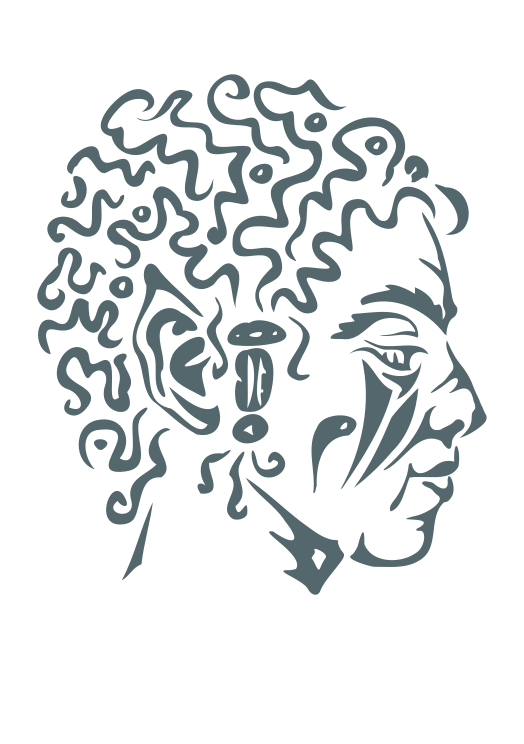
\includepdf[pages={1}]{pic_MitchoeOldBook.pdf}
\newpage
\thispagestyle{plain}

Митхэ ар'Кахр, авторства предположительно жреца Саритра ар'Кахра э'Кахрахан.
Рисунок чернилами в книге <<Мстительные тени>> редакции 10130 дождя, принадлежавшей Людям Золотой Пчелы.
% ----- PICTURE: MITCHOE -----

\chapter{[-] Бумажный фонарь}

\section{[-] Посохи}

Путники с бумажными фонарями --- особое общество.
Кто-то из них знает, что посвящён Сату-скитальцу, кто-то интуитивно повторяет привычки знакомых.
Сели, хака, ноа, ркхве-хор, зизоце, трами, травники, совсем редко --- дикие идолы с татуированными лицами.
Посохи ркхве-хор похожи на срубленные и слегка ошкуренные деревья.
Когда великаны кланяются, их посохи ощутимо скрипят.
Посохи травников едва годятся для того, чтобы ворошить костёр;
этот народ приветливо щёлкает челюстями и поднимает четырёхпалые руки горе.
Но все они --- одно: мы не мёртвы, не живы, мы в пути.

Вот навстречу попалась женщина-хака.
Молодое лицо с неглубокими морщинками, серые глаза, длинные дреды, сплетённые из её собственных волос и волос случайных попутчиков.
Штаны сели, красивая пылеройская накидка, чересчур широкая ей в плечах.
На родине женщину признали бы негодной и подвергли остракизму.
Но здесь, на дороге, властвует бумажный фонарь.
Мы встретились взглядами... как вдруг усталое лицо расцвело искренней щербатой улыбкой, и я неожиданно для себя улыбнулся в ответ.

Едем дальше.
Ни имени, ни привета, да и лицо прохожей уже расплывается в памяти, но вечернее небо на миг стало более голубым.

\section{[-] Совпадение}

\textspace

Дорогу вальяжно перешла недавно опоросившаяся самка дикобраза.
Выводок семенил вслед за ней.
Увидев повозку, самка повернулась к ней задом, с костяным треском встряхнула иглами и затопала, словно строй маленьких копейщиков.

Чханэ придержала оленей и подождала, пока дикобразовое семейство не уйдёт восвояси.

--- Плохая примета, --- пробурчала она и, подхватив чётки Сата, начала сосредоточенно искать узлы.
--- Лис, давай-ка просёлками поедем, поворот в паре кхене отсюда.
Как бы на засаду не нарваться, ни к чему нам сейчас это...

Я кивнул.

Извилистая тропинка, несмотря на дождь, оказалась в удивительно хорошем состоянии.
Мы оставили за плечами хутор, затем ещё один...
Судя по лежащему на обочине, почти заросшему землёй верстовому столбу, до дороги на Травинхал оставался один кхене.

Тропинка сделала крутой поворот, обнимая серую с чёрными крапинками скалу.
Я дёрнул поводья, и олени встали как вкопанные.

--- Не может быть... --- ахнула Чханэ.

Я не ответил.
Такое везение действительно бывает раз в жизни.

Прямо перед нами развернулся маленький палаточный лагерь.
Горели костерки, в походных котлах булькало что-то съестное.
Неподалёку паслись стреноженные олени.
А в двадцати шагах от нас, на воткнутом в землю копье трепетало на ветру перештопанное знамя.

Жёлтая пчела на тёмно-зелёном фоне.

\section{[-] Золотая Пчела}

\epigraph
{Даже над старой тропой светит сегодняшнее солнце.}
{Пословица сели}

Первый жрец назначил мне встречу глубокой ночью.
Чханэ и мальчики уже давно спали в палатке.
Митхэ оживлённо болтала со старыми жрецами, которых мучила бессонница;
кажется, они играли в какую-то игру.
Костры медленно, с тихим шипением умирали под моросящим дождём.

--- Когда-нибудь я стану жрицей! --- донёсся до меня гордый возглас девочки.
Старые жрецы восхищённо заохали.

<<Может, оставить её с ними? --- подумал я.
--- Бродячему Храму необязательно приносить жертвы...>>

Первый жрец застегнул клапан шатра и неторопливо, одну за другой разжёг четыре масляных лампы.

--- Твой ребёнок очень серьёзно настроен, --- сказал он.
--- Ты хорошо её воспитал.

--- Митхэ --- не мой ребёнок, --- сказал я.
--- Нас свёл случай.

--- А разве иначе бывает? --- усмехнулся жрец.
--- Даже если один человек вылез из другого, их всё равно свёл случай.
Все знакомства равноценны в самом начале и лишь потом обретают индивидуальность.
Так или иначе, мне девочка сказала, что ты --- её кормилец.

Я смутился.

--- У меня к вам есть необычная просьба.

--- Мы её не возьмём, --- предупредил вопрос Первый.
\ml{$0$}
{--- У нас, в отличие от городских, нет никаких предубеждений по поводу женщин, это вопрос милосердия.}
{``We're not prejudiced against women, unlike city priests---it's a matter of charity.}
\ml{$0$}
{Её бремя и так достаточно велико, чтобы взваливать на ребёнка ещё и тяготы жизни бродячего жреца.}
{The child's own burden is heavy enough to be carried with a burden of wandering priest on top of that.''}

--- Благодарю за гостеприимство, --- сказал я.
--- Мы несказанно рады, что обнаружили вас здесь.
Мне сказали, что вы отправились за море, в земли ноа.

--- Да, мы действительно собирались идти в земли ноа, --- кивнул жрец.
--- К сожалению, Кипящее море сейчас штормит, пришлось немного изменить маршрут.
Зашли в Хатрикас, затем по землям хака прошли на Север.

--- Хака вас пропустили? --- удивился я.

--- У них было много больных, они не возражали против нашей помощи.

Я промолчал.
Первый жрец стоял и прислушивался к шуму дождя;
он явно не торопился начинать разговор.
Наконец, спусля несколько михнет, мой собеседник нарушил молчание.

--- Прошу прощения, --- сказал он.
--- Я должен был убедиться, что ты не привёл за собой хвост.
Мне только что сообщили, что всё чисто.
Мы можем говорить свободно.

--- Я так понял, вы уже обсудили письмо.

--- Мы его прочитали, --- кивнул Первый.
\ml{$0$}
{--- Оно многое объясняет.}
{``Many things were explained.''}

\ml{$0$}
{--- Многое?}
{``Many things?''}

--- Аспекты сегодняшней общественной жизни в землях сели.
\ml{$0$}
{Перечислять долго и незачем.}
{There's no time nor reason to enumerate.''}

--- Вы опросите людей, чьи имена указаны в письме?

--- Среди людей Золотой Пчелы есть бывший Первый жрец Тхитрона.
Он знал Трукхвала ар'Хэ лично и подтвердил его почерк.

\ml{$0$}
{--- Бывший Первый жрец Тхитрона?}
{``Former Head priest of \Tchitron?}
\ml{$0$}
{Можно узнать, кто именно?}
{May I ask, who exactly?''}

\ml{$0$}
{--- Я.}
{``Me.''}

--- Как так вышло?

--- Долгая и запутанная история, как и у тебя.
Некоторые из моих жрецов до последнего времени вели с Трукхвалом переписку, и твоё имя там упоминалось неоднократно.
Мы слышали и о тхитронской диверсии.
Кроме того, мы осведомлены обо многих странных событиях, в том числе и в указанных двух Храмах.
\ml{$0$}
{На первое время этого достаточно.}
{That's enough for a while.}
Что ж, Ликхмас.
Скажи, сколько сейчас жрецов в Тхитроне?

--- Сейчас --- не знаю.
Перед уходом мы с Трукхвалом и моей женщиной перебили всех чужих.

--- Всех? --- поднял брови Первый жрец.

--- Я понимаю, что мы оставили город без защиты.
Но произошло это во время жертвоприношения, и жертва была принесена по всем правилам.
Мы оставили Храму время для действий.

\ml{$0$}
{--- Я прошу прощения.}
{``I beg your pardon.}
Просто Трукхвал, насколько я знаю, тихий миролюбивый хромец, да и вы с Тханэ ар'Катхар не производите впечатление людей, решающих проблемы силой.
Видимо, вам и правда пришлось туго.
\ml{$0$}
{Я так понимаю, что ты вне закона?}
{If I understand right, you are outlaw now?''}

\ml{$0$}
{--- Я не знаю точно, но скорее всего да.}
{``I don't know for sure, but more than likely yes.}
\ml{$0$}
{Воительница из моего Храма сообщила, что был отдан приказ брать нас живыми или мёртвыми.}
{A warrior from my Temple told me that she were ordered to take us dead or alive.''}

--- То есть ты связывался с Нижним Этажом?

--- Старые воины помогли нам бежать.
Среди них есть те, кто поддержал нового Первого жреца, но я не думаю, что они сделали это из корыстных побуждений.
Новые жрецы отлично умели запугивать и убеждать.

\ml{$0$}
{--- Охотно верю.}
{``I do believe.}
Мне рассказывали, что их дар убеждения граничит с колдовством, и бесхитростные люди очень часто попадают от них в зависимость.
\ml{$0$}
{Трукхвал погиб в бою?}
{\Trukchual, was he slain in fight?''}

\ml{$0$}
{--- Я забрал это письмо с его тела.}
{``I took this letter from his body.''}

\ml{$0$}
{--- Сочувствую.}
{``I'm sorry.}
Кстати, из какого ты дома?

--- Я хранитель Митхэ ар'Кахр, воспитывался в доме купца Кхотлам ар'Люм.

--- Кхотлам жива?

--- Жива.
Она до сих пор купец Тхитрона.
Вы её хорошо знаете?

--- Чересчур хорошо, --- ухмыльнулся Первый.
--- Это сейчас она остепенилась, ведёт жизнь примерного городского купца, но в молодости она натворила делов.
Скажем так, она ценила справедливость чуть больше, чем мир --- неудачное качество даже для очень умелого дипломата.
На этой почве она, например, хорошо подружилась с отрядом чести Митхэ ар'Кахр, и те не раз нам помогали почти бесплатно.
Один из её пассажей расхлёбывать пришлось мне.
К моему вящему неудовольствию, взвесив все за и против, я понял, что для Тхитрона она гораздо полезнее меня.
Первого жреца найти --- раз плюнуть, а вот таких дипломатов в канаве не найдёшь.

--- Ты справился?

--- Если она до сих пор на посту --- полагаю, что да, она сделала выводы и изменила стратегию.
Ещё одно доказательство, что я в ней не ошибся.
В целом вопросов у меня больше нет.
Бери пергамент и пиши.

Жрец дождался, пока я разложу письменные принадлежности на столике, и начал диктовать:

--- <<Трёхэтажному Храму от людей Золотой Пчелы>>.
Дату поставь послезавтрашнюю.

\begin{quote}
<<Мы знаем, что в землях сели действует группа жрецов, которая совершает перевороты в городах с целью захвата власти.
Возможно, что эта группа в настоящий момент контролирует абсолютное большинство Храмов.
Пусть всё остаётся так, как есть.
Мы не хотим войны и волнений.
Тем не менее, ввиду некоторых обстоятельств, мы вынуждены требовать, чтобы рекомая группа уступила людям Золотой Пчелы Храм Тхитрона.
В противном случае мы обнародуем сведения о деятельности рекомой группы со всеми вытекающими последствиями>>.
\end{quote}

Я поднял голову.

--- Это будет означать гражданскую войну.

\ml{$0$}
{--- Именно.}
{``Exactly.}
\ml{$0$}
{Они на это не пойдут.}
{They wouldn't allow that.''}

--- А что, если им нужна гражданская война?

--- Война войне рознь, Ликхмас.
Они могут стравливать между собой города и сословия, что они и делают сейчас.
Но поверь, \emph{такая} гражданская война им ни к чему.

--- Написал.

--- Отлично.
А теперь перепиши это письмо ещё раз.
Одна копия отправится во Двор Люм вместе с оригиналом письма Трукхвала.

Я вытащил второй листок пергамента, мимоходом восхитившись опытом Первого жреца.

--- Тебе был нужен мой почерк.

--- Безусловно, женщина, которая воспитала ребёнка, узнает его почерк.
Думаю, она будет рада узнать, что ты с нами.

--- Вам будет грозить опасность.

--- <<В жизни и смерти я буду щитом>>.
Это для вас, храмовников, опасность --- что-то из ряда вон выходящее.
Для людей Золотой Пчелы это обыденность --- договариваться, обходить чужие ловушки.
Я бы предложил тебе присоединиться к нам, потому что такой опыт на дороге не валяется.
Но времена, увы, не располагают.
Насчёт Храма не волнуйся --- кто бы это ни был, они уверены в победе.
Тхитрон нам уступят, считая, что это временная мера.
А маленькие бескровные победы всегда тянут за собой большую.

--- С Тхартхаахитром всё понятно.
Но примут ли тхитронцы тебя обратно, учитывая твою биографию?

--- Сейчас у них нет выбора.
Ворчать будут однозначно.
Я уверен, особо горячие головы даже разобьют пару окон в здании храма, чтобы напомнить мне, кто я есть.
Но на этом всё и закончится.

--- Что потом?

--- Потом --- чистая дипломатия.
Мы намекнём Тхартхаахитру, что просто хотели урвать свой кусок пирога из общей миски.
Людям, которые мыслят одинаково, проще договориться.
Поэтому нужно уметь думать по-другому.
Ты идейный человек, потому тебя и изгнали.
Они поняли, что с тобой нельзя договориться способами, которые им понятны --- подкупом, обманом или запугиванием.
Для них, жаждущих власти и благ, твой образ мышления --- чуждый, непонятный, а значит --- опасный.

--- Интересно, что их агентов нет среди вас.

--- Ты в этом уверен?

--- Уверен.
Я уже научился их отличать.

Первый жрец почесал щёку.

--- Нам с тобой ещё надо будет пообщаться, Ликхмас, но не сейчас, конечно же.
А насчёт агентов...
Эти люди хотят власти.
А какая власть у нас, у Бродячего Храма?

Я посыпал пергамент песком, поднялся из-за стола и протянул листки собеседнику.

--- Благодарю тебя.
Я рад, что оставляю Тхитрон в надёжных руках.

--- Рано благодарить.
Поблагодаришь, когда вернёшься в родной Храм.
\ml{$0$}
{Тебя будут ждать.}
{You will be welcome.''}

\ml{$0$}
{--- Я не могу вернуться.}
{``I can't return.}
\ml{$0$}
{Есть дела.}
{I have things to do.''}

К моему удивлению, он не стал задавать вопросов.

--- У вас провианта на день, --- подумав, сказал жрец.
--- Мы выдадим вам, сколько сможем, потому что в дождливые сезоны Север не склонен быть гостеприимным.
Сегодня ночуем вместе, а завтра на рассвете люди Золотой Пчелы идут в Тхитрон.
\ml{$0$}
{Ну и на всякий случай.}
{And, just in case.}
\ml{$0$}
{Я не знаю, что ты задумал, но можешь на нас рассчитывать.}
{I've no idea what you're up to, but you can count on us.''}

\asterism

Вскоре обстановка разрядилась.
Первый жрец заварил травы и достал откуда-то мешочек с конфетами, пряными и обжигающе-холодными на вкус.
Мы пили отвар и рассказывали друг другу истории из жизни.

--- Ты не поверишь, как приятно общаться с молодыми жрецами, --- улыбался Первый.
--- У нас молодёжи не было уже много дождей.
Наш Храм стареет.

--- Я думал, что Бродячие Храмы остались лишь в легендах, --- признался я.

Первый хохотнул.

--- И не ты один.
Ты же ведь знаешь, почему Бродячие Храмы в итоге исчезли?

--- Нет, не знаю.

--- Немудрено.
В поселениях об этом стараются не упоминать.
Но про гибель отряда чести Митхэ ар'Кахр ты наверняка знаешь.

--- Я встречался с ней в землях хака.
Митхэ обвинили в убийстве жреца.

--- Хай, так она жива? --- удивился Первый.
--- Сильная женщина.
У нас где-то в походной библиотеке хранится книга с её портретом на форзаце, старая-старая гравюра по коже...

Первый поднялся на ноги и зазвенел ключами.
Найдя нужный, он открыл походную библиотеку и вытащил на свет книгу.
Слабый тёплый свет масляной лампы выхватил потускневший профиль на покрытом пятнами форзаце.

--- Наверное, ты видел её не в лучшие дни её жизни.
А вот такой она была.
Маленькая, красивая и гордая, искреннее и смелое сердце.
Она происходила из южан, но северяне в ней души не чаяли.
Кстати, повернись-ка...
да, ты на неё очень сильно похож.

\ml{$0$}
{--- Я знаю.}
{``I know.}
\ml{$0$}
{Такой же мелкий и проблемный.}
{The same small trouble-maker.''}

Первый усмехнулся и передал книгу мне.

--- Да, она многим успела насолить, сама того не желая.
Дело было спланировано заранее, и принимал в нём участие не только Трёхэтажный Храм.
Издревле Бродячие Храмы были чем-то наподобие кузницы, в которой ковалось жречество и воинство, эдакой сокровищницей на крайний случай.
Если в каком-то из городов Храм переставал выполнять свою роль, заменяли его именно люди из Бродячих Храмов.

Я кивнул.
Мозаика сложилась полностью.

--- Борьба за власть?

--- Именно.
Началась она не сегодня и не вчера.
В прежние века мы приносили праздник в города, собирали целые толпы народа, давая возможность городским храмовникам наконец-то выспаться, выпить по чаше чего-нибудь и съездить в отпуск.
Городские жрецы лечились у нас, воины тренировались с приезжими, хотя чаще просто оставляли на них город.
Ведь это же здорово --- довериться знающему человеку, а не думать самому, что да как.
Но со временем, как видно, мы стали для городских не сменой и подмогой, а напоминанием, что они --- легкозаменимые детали механизма.

Жрец снова усмехнулся.

--- Вначале города стали различными способами ограничивать деятельность Бродячих Храмов.
Нам для лагеря начали выделять самые глухие места за городом.
Порой люди даже не знали, что мы рядом.
Затем начались проволочки с перемещениями --- воины учиняли допросы, задерживали и изменяли наш маршрут под разными предлогами.
Например, мой предшественник --- да хранят духи его покой! --- рассказывал с горьким смехом, как его не пропустили в деревню, охваченную эпидемией.
По какой причине, спросишь ты?
Потому что карантин!
Жреца не пустили из-за карантина!
Если бы это мне рассказал кто-то другой, я бы не поверил.

Первый закрыл лицо руками и покачал головой.

--- Из-за отсутствия заработка Бродячие Храмы начали редеть.
Некоторые осели, были и те, кто занялся торговлей.
На моём веку один Бродячий Храм стал бродячим театром --- и это ещё не самая неприятная метаморфоза, потому что именно как результат такой политики тогда начался всплеск разбоя и наёмничества.

--- В моём детстве о разбойниках говорили постоянно, --- припомнил я.
--- Так это?..

--- Бывшие воины, Ликхмас.
Воины, которых фактически оставили без средств к существованию.
Кто ещё обладал достаточным количеством опыта, чтобы обводить вокруг пальца храмовников?
В Бродячих Храмах остались в итоге лишь идейные люди, готовые к трудностям.
Да, были те, кто выжил, кто научился обходить ловушки и решать проблемы, которые устраивали городские Храмы.
Как будто своих проблем не хватало...
Когда отряд чести Митхэ перебили, это было сигналом именно для них --- оставшихся.
Людям Золотой Пчелы пришлось в итоге заключить с Тхартхаахитром негласный договор --- мы не вмешиваемся в дела городов, а нам дают немного зарабатывать.
Вот так, Ликхмас.
Это перештопанное знамя знавало лучшие времена...

--- Ты ведь давно ждал этот момент, не так ли?
Момент, чтобы вмешаться?

Жрец улыбнулся и промолчал.

\section{[-] Встреча с Грейсом}

Ихслантхар встретил нас неприветливо.
Дождь, грязь по щиколотку.
Едва найдя постоялый двор, мы поняли, что лучше остановиться у кого-нибудь из горожан.
Двое или трое вежливо отказали, сославшись на тесноту, ещё десять были гораздо менее вежливы, но подавляющее большинство даже не откликнулось на <<гостевой>> стук.
Пришлось вернуться на постоялый двор.

Хозяин, в противоположность горожанам, оказался на удивление вежливым и отзывчивым человеком.
Однако его вежливость и отзывчивость стоили дорого;
не встреть мы Людей Золотой Пчелы, которые пополнили наш провиант, пришлось бы совсем туго.

--- У нас не хватит золота надолго здесь остаться, --- резюмировала Чханэ.
--- Сколько времени тебе потребуется, чтобы найти друга?

Я промолчал.
Поиск товарищей всегда был проблемой;
пробуждённые, разумеется, узнавали друг друга сразу, но спящего демона засечь практически невозможно.
Тем не менее способ был.
Демон даже в спящем состоянии заставляет тело совершать некие стереотипные действия --- так называемые МПС\FM, которые могут выдать его союзникам.
\FL{mbs}{Маркерные поведенческие стереотипы}
Я с сожалением посмотрел на стену дождя за окном.
Разумеется, все жители сидят по домам.

Наступила ночь.

Первой ушла спать Чханэ, уведя мальчиков.
Митхэ сидела со мной.
Вскоре её разморило, и девочка заснула у меня на коленях, разлив по полу отвар.
Зал постепенно опустел, но хозяин стоял у стойки, словно кого-то ожидая.

Вдруг колокольчик у дверей зазвенел, и в зал вошла грустная, немного сутулая молодая женщина.

--- Тебе как обычно? --- вскинулся хозяин.

--- Добавь ещё перца, --- попросила женщина.

Женщина не глядя опрокинула в себя три чаши крепкого пива с перцем, закусила орехами и заплакала.

--- Опять? --- сочувственно сказал хозяин.

--- Он меня вообще не слушает, --- тихо прорыдала женщина.
--- Бормочет ночами, а сам...
Как будто я не существую.

--- Тхартху, позови всё-таки жрецов, --- посоветовал хозяин.
--- Это уже не дело.
Секхар всегда был чудным, но сейчас с ним явно что-то не в порядке.

--- Прошу прощения, --- поднял я руку.
В пустом зале слова отозвались эхом, и собеседники вздрогнули.

--- Вам что-то ещё? --- спросил хозяин.

--- Нет-нет, --- покачал я головой.
--- Просто так вышло, что я жрец.
Не храмовый, путешествую.
Если нужна моя помощь, я помогу.

--- Я не смогу оплатить твои услуги, --- сказала женщина.
--- Храмовники сделают всё бесплатно, и...

--- И по какой-то причине ты до сих пор к ним не идёшь, --- подхватил я, --- а изливаешь печаль трактирщику.

--- Это мой брат, --- с укором сказала женщина.
--- Как ты смеешь!

--- А пиво --- твоя сестра.

--- Что?

--- Тебя выдают жесты, вышивка-оберег подмышкой и чётные слоги, растянутые и извилистые, как истоки Рек-Близнецов.
А у твоего собеседника городские манеры и чистый столичный выговор, более присущий пожилым, нежели людям его возраста.
Если не хочешь, чтобы я лез в твои дела --- так и скажи.
Только не надо врать.

Женщина сжалась и бросила взгляд на хозяина.
Тот отвернулся и сделал вид, что протирает посуду.

--- Приюти меня, мою женщину и троих детей на полдекады, --- сказал я.
--- Как видишь, мы тоже переживаем не лучшие времена.

Тхартху снова бросила взгляд на хозяина, но тот, видимо, решил больше не вмешиваться.
Наконец женщина кивнула.

--- Пойдём со мной.

--- Я присмотрю за девочкой, --- добавил хозяин и кивнул мне.
Я аккуратно положил головку спящей Митхэ на скамью и укрыл потеплее плащом.

Улица, поворот, улица, поворот, улица, поворот...
Я уже начал подозревать, что Тхартху наивно пытается запутать меня.
Но вот по левую руку появилась кузня.
Прошлёпав в грязи, мы поднялись к красивой узорчатой двери.

Всего одна лампа освещала жилище.
Это было не пламя;
в обычном фонаре весело жужжал настоящий маленький светодиод.
У верстака сидел и клевал носом высокий мужчина с небольшим брюшком.
Длинные спутанные <<рыбки>> с металлическими кольцами подмели столешницу, когда он обернулся к вошедшим.

--- Наконец-то, --- проворчал низкий голос знакомыми интонациями.
--- Я тебя заждался.

Я без слов подошёл и заключил его в крепкие объятия.

\asterism

--- Еда ещё осталась.
Вот суп сварил, --- бормотал Грейсвольд.
--- Птичка, кушай, малышка.
Прости, что я так с тобой обращался последнее время, но по-другому я просто не мог послать Аркадиу сигнал.
Долго объяснять.
Ты как сам-то, дружище?
На улице жуткая погода.

Тхартху с круглыми глазами, почти не слушая, хлебала томатный суп.

--- Грейс, что случилось? --- спросил я.
--- Ты получил мой сигнал о пробуждении?
К чему эти игры в домики-дороги?

Грейсвольд покряхтел и сел за стол.

--- Получить-то получил, но я сам напортачил с пробуждением, --- сказал он.
Говорил друг на языке тси --- видимо, хотел, чтобы Тхарту тоже поняла часть разговора.
--- Чувствуешь?
Весь дом в технике.
Всё, что можно, против отслеживания.
Можешь осмотреть, только осторожно.

Я <<осмотрел>> жилище.
Наноустройства были везде, в каждом камне пола, в каждой доске стены.
Чтобы сделать такое количество, нужно...

--- В общем, ты понял, да, --- вздохнул технолог.
--- Я почти без энергии.

--- Как так вышло?

--- У меня во время пробуждения начался акбас.
Самый настоящий, со спецэффектами.

--- Ты потерял над собой контроль? --- удивился я.

--- Да, --- кивнул технолог.
--- У тебя подобного не было?

--- Нет, --- покачал я головой.
--- Хотя постой...

Я вспомнил Чханэ.
В голове промелькнули алтарь, пробуждение и странная борьба тела и демона, которой никогда раньше не бывало.

--- У нас большие проблемы, Аркадиу, --- глухо резюмировал технолог, словно читая мои мысли.
--- Что-то происходит, не только вокруг, но и внутри нас с тобой.

Технолог выразительно коснулся пальцем виска.

--- Ну ты же знаешь, что обычно происходит при акбасе.
Всё концентрируется на одной мысли --- надо срочно обезопасить себя, любой ценой, любыми доступными средствами.
В общем, результат был прямо противоположным --- засветился я по полной.
Агенты Картеля встали на уши.

--- Блеск, --- буркнул я.

--- Я не мог послать вам сообщение раньше, --- развёл руками Грейсвольд.
--- Пришлось надеяться на твою смекалку.

Грейсвольд кивнул на Тхартху.

--- Она меня очень любит.

--- И поэтому ты вынудил её ходить в постоялый двор за выпивкой?
А сказать нельзя было?

Грейсвольд выглядел ошеломлённым.

--- Моя женщина знает, --- добавил я.

--- План не на той стадии, когда можно доверять всем подряд.

--- <<Всем подряд>>? --- процедила Тхартху.

Грейсвольд бросил виноватый взгляд на подругу.
Та сидела, скрестив руки на груди и глядя в стену.

--- Пять дождей, Секхар, --- голос Тхартху дрожал.
--- Пять дождей моей любви, но я по-прежнему <<все подряд>>.

Мы промолчали.
Тхартху грустно усмехнулась и встала.

--- Очень рада, что ты <<выздоровел>>.
Похоже, для меня пришло время показать, что хотя бы в Ближнереках люди верны своему слову.

Она повернулась ко мне.

--- Я приготовлю места и завтрак тебе, твоей женщине и детям.
Повтори только, как тебя зовут, я не разобрала.

--- Зови меня Ликхмас ар'Люм э'Тхитрон.
Или Играющая-Камнем-Лиса.

--- Женщине?
Детям? --- удивился Грейс.
--- Ты сюда выводок притащил?

--- Так вышло, --- развёл я руками.
--- Мы оба хороши.

--- Нет, вообще очень умно.
Агенты обращают меньше внимания на семейных, демоны чаще одиночки.

--- Всё, забыли, --- прервал я его.
--- Главное --- все живы, остальное приложится.
Пойду приведу своих.
Тхартху старалась меня запутать, но не учла, что постоялый двор у вас видно из окна.

Женщина густо покраснела.

--- Ликхмас, сейчас ночь, --- осторожно заметила она.
--- Я думаю, не стоит будить детей ночью.

--- Если переезжаешь в хороший дом, подойдёт любое время, --- ответил ей Грейсвольд.
--- Ложись-ка ты тоже спать, у тебя ещё пиво в глазах плещется.
Я сам приготовлю лежанки.
Как тебя зовут, Аркадиу?
Ликхмас, точно, только что прозвучало.
Сколько детей?

Я показал ему большой и указательный палец, затем направился к двери.

\ml{$0$}
{--- Десять тысяч дождей, а мозгов нет, --- резюмировал технолог мне вслед.}
{``Ten thousand rains, has got no brains,'' the technologist summed up to my back.}
--- И когда только успел троих настрогать!
Две пяди в обхвате, от макушки до пяток --- кукурузный початок, а стручок уж дорогу в амбар знает...

\section{[-] Живите кто хотите}

Перед уходом Грейсвольд долго стоял и гладил резную колонну жилища.
Жилище было совершенно не похоже на прочие, стоявшие на улице.
Я был уверен, что подобного ему не нашлось бы и во всём Ихслантхаре.

--- Это хорошее жилище, --- сказал Грейс.
--- Мы с Тхартху строили его вместе.
Резьба и рисунки полностью принадлежат её рукам.

--- Оно выглядит точь-в-точь как в моих детских мечтах, --- улыбнулась женщина.
--- Ликхэ-лехэ делал конфетные дворцы, и я ребёнком часто забегала к нему в лавку, смотрела на них и думала, что я хочу такой домик.

Грейсвольд бросил на неё смущённый взгляд:

--- Может, всё-таки останешься?
Тебе ничего не грозит.

--- Без тебя мне здесь делать нечего, --- отрезала Тхартху.
--- Так что хватит об этом.

--- Как скажешь.

--- Мы уходим навсегда.
Надо отдать дом сельве, чтобы путь был безмятежным и удачным.

--- Надо, --- признал Грейс, --- но у меня рука не поднимется.

--- У меня тоже, --- призналась Тхартху.
--- Что ж...

Женщина вытащила из-под навеса чистую коротенькую доску и положила на скамью.
В её крепких руках заплясал кукхватровый резец, разбрасывая деревянные кудряшки и коротенькие щепочки во все стороны.

--- Хорошая идея, --- похвалил Грейс, оглядев работу.
--- Поставь её на рога наличника, вон туда.
Там она будет держаться крепко и её увидят все.

--- Отдавать людям даже лучше, чем отдавать сельве, --- улыбнулась Чханэ.
--- Это не будет забыто.
Пусть жилище принесёт радость новым хозяевам.

Мы аккуратно прикрыли калитку и, бросив последний прощальный взгляд на жилище, отправились по размытой дороге на юг.

Фонарь у двери остался гореть, освещая прихотливую резную надпись:

<<Дом свободный, живите кто хотите>>.

\section{[*] Одинокий Столб}

Одинокий Столб можно было назвать городом с большой натяжкой --- он едва насчитывал полторы сотни строений, включая храм, гостиницы и исторические здания.
Тем не менее он представлял из себя настоящую крепость, ограждённую стеной.
Это была не символическая стена, подобная той, что в Тхитроне;
качество этой стены может продемонстрировать один простой факт --- она не пригодилась ни разу.
Даже Молчащие идолы, издалека осмотрев укрепления крохотного города, взвесили риски, оценили возможную выгоду --- и благоразумно обошли святилище стороной.

В темноте при взгляде с дорог или реки Одинокий Столб казался леденцовым дворцом --- ажурные венцы башен и кромка стены сияли от света оранжевых хрустальных тыкв, внутри которых пылал настоящий природный газ.
Хитроумное древнее приспособление отводило газ от окружающих святилище болот;
за день его собиралось достаточно, чтобы тыковки пылали всю ночь.

Название святилищу дал, как можно догадаться, Столб --- один из четырёх талисманов города.
По поводу возраста Столба шли ожесточённые споры, но ни у кого не вызывало сомнений, что он был возведён самими Древними.
Столб был сделан из неизвестного материала, похожего на белоснежно-чистый фарфор, оплетённый кукхватровыми кольцами.
Как и стена, Столб имел хрустальные окошки, и они также светились по ночам, но как и зачем --- не знал никто\FM.
\FA{
Главной реликвией Одинокого Столба является надземный модуль (маячок) золотодобывающей установки тси.
Как показало исследование устройства, оно прекратило работу за пять тысяч лет до описываемых событий, перейдя в режим ожидания.
В настоящее время Столб признан культурно-исторической ценностью планеты Тра-Ренкхаль и подлежит охране.
}

Прочими тремя талисманами города были тысячелетний молчащий кедр, Запретная роща --- роща благородного баньяна, а также развалины Су'макхэтхвал --- пятнадцать древних землянок, первое поселение возле Столба.
Каждая реликвия находилась в своём квартале: Столб --- в Верхнем Приозерье, Кедр --- в Квартале Кедра, Су'макхэтхвал относился к Кварталу Снежных Бород, а Запретная роща была в ведении Большого и Малого Домов.
При этом любые две реликвии разделяло не более ста шагов.

\section{[*] Никто}

Воинов в святилищах нет.
Есть только стражники.
Стражники приносят немного другую клятву.

--- Ты фыпрала хороший тень, штопы пройти шерес эти форота, Митхэ ар'Кахр, --- улыбнулся стражник.
Несмотря на строгое соблюдение правил северного диалекта, слова он выговаривал нежно, приглушённо и протяжно, сливая некоторые похожие звуки в один;
этот акцент --- <<шёпот любовника>>, или <<голубиное воркование>> --- был верным признаком коренного жителя святилища, но многие сели по незнанию могли счесть его носителя иноплеменником.

--- Здравствуй, Трасакх, --- коротко ответила на приветствие Митхэ.

--- Эрхэ ар'Люм, Акхсар ар'Лотр, --- Трасакх прищурился, разглядывая Ситриса, --- и Ситрис ар'Эр.

Ситрис вздрогнул.

--- Ты меня знаешь?

--- Ни ф коем слушае, --- строго сказал стражник.
--- Орушие --- полнорасмерное, киншалы, стрелы, лесфия --- в корсину.
Саколки, пишутерию и фстроенное ф отешту мошно остафить, --- добавил он, услышав тяжкий вздох Ситриса.
--- Каштый пусть сам кормит сфои страхи.

--- А лук?
Ружьё? --- удивился Акхсар.
--- Раньше забирали стрелковое.

--- Хай, мы потумали и решили, што тостатошно сапирать поеприпасы, --- развёл руками стражник.
--- Ресультат тот ше, а на склатах теперь мноко места.
Но если ты путешь пить кофо-то луком, я ефо тоше саперу.

Спутники Митхэ сложили оружие в большую плетёную корзину.
Митхэ, поколебавшись едва ли мгновение, вынула кинжал, затем положила в корзину саблю.

--- Хай, у тепя нофая сапля? --- удивился стражник, затем вытащил её из корзины и осмотрел.
--- Красифая.
Слушайно не рапота Секхара ар'Митр э'Сотрон?

--- Его, --- улыбнулась Митхэ.

--- Стиль ошень уснафаемый, хотя послетнее фремя, по слухам, крафирофкой санимаются ефо маленькие тети.
Я перетам её на хранение ф Польшой Том.

--- Почему туда? --- насторожилась воительница.

--- Так нато, Митхэ ар'Кахр, --- строго ответил стражник.
И полушёпотом добавил:
--- Тела и саконы сели нас касаются ф той ше мере, што и фсекта.
А фот форы к нам сашастили.
Орушие шресфышайно сенное, и я настоятельно рекоментую сокласиться с этой мерой претосторошности.

--- Хорошо.

--- Неуютные нынше фремена, --- вздохнул стражник.
--- Усомнилась ли пы ты фо мне тоштей тфатсать насат?

--- Прости, --- поклонилась Митхэ.
--- На мою долю за последнее время выпало слишком много.

--- Мы слышали, --- кивнул мужчина.
--- Кстати, не шти слишком мнокофо от Ссепленных Рук.
Сейшас у них ф колофах поттершание не мира мешту наротами, а фитимости сопстфеннофо нейтралитета.

Тон стражника сквозил презрением;
на памяти Митхэ Трасакх никогда не позволял себе так отзываться о собственном Храме.
Митхэ и Эрхэ переглянулись.

--- Что ты имеешь в виду? --- спросил Акхсар.

--- Ты не найтёшь кофо-то, кто помошет тепе с Атрисом, Акхсар ар'Лотр, --- без обиняков пояснил стражник и открыл ворота.
--- Поэтому, если хошешь помоши, проси её у никофо.
Никто, как ни утифительно, фсекта ф курсе сопытий.
В катакомпах мноко этих никофо, и периотически ис-са них мы шефо-то нетосшитыфаемся.
Например, хороших сапель.
Храни фас Сит.

\asterism

То, что стражник назвал <<катакомбами>>, на самом деле было целым городом, но уже подземным.
Вернее, аж двумя городами --- хйяр Тар и хйяр Катх\FM, общая площадь которых превышала площадь самого Одинокого столба в полтора раза.
\FA{
Хйяр Стариков и Паучий Хйяр.
}
Концентрические пещеры\FM, центром которых был всё тот же Столб, за прошедшие тысячелетия поросли кальцитовыми натёками, и когда-то давно в них решили сделать жилища.
\FA{Результат работы золотодобывающей установки.
Устройство пропускало через породу продольные волны, облегчавшие процесс добычи.
}
Пока не выяснилась неприятная деталь --- при наличии хотя бы одного слабого места с болот в систему пещер поступал тот самый газ, делая нижние этажи подземных городов непригодными для жизни.
Вначале с этим пытались бороться, но природа взяла своё.
На хйяр Тар и хйяр Катх махнули рукой, и они теперь лишь изредка поражают красотой приезжих, достаточно смелых, чтобы спуститься в разлом.

Жили в подземельях и воры.
Это было крайне редкое занятие в землях сели --- честным трудом можно было заработать проще и быстрее.
Поэтому ворами становились либо совсем юные беспризорники, либо идейные люди, которые не могли представить жизнь без риска, либо кутрапы, которых ждала смерть в любых уголках Короны.
Причём беспризорники, повзрослев и получив метку за Насилие, чаще всего просто уезжали подальше и начинали новую жизнь, благо такая возможность представлялась ещё много раз --- пока человек не совершал преступление в пределах нового города, он был для него чист и честен.
Формально.
Люди же, несмотря на все увещевания дипломатов, заранее настороженно относились к человеку с метками трёх-четырёх городов.

В Одиноком Столбе воры жили очень тихо, воровали в основном пищу и одежду, аккуратно и помалу, так как знали --- если дать повод стражникам заняться катакомбами, то катакомбы опустеют надолго.
Заблудившимся в подземельях приезжим воры часто устраивали экскурсии за золото или по крайней мере показывали дорогу наружу.
Именно поэтому их не трогали и на воровство смотрели сквозь пальцы.

<<Под землёй растут лишь грибы, а из грибов лепёшки плохие>>, --- говорили жители святилища, если речь заходила о разломах.
Очень часто хйяр Тар и хйяр Катх были единственным местом, где мог жить кутрап.
Кое-кто из жителей специально оставлял пищу и одежду на видном месте.
А раз в декаду местные жрецы отправлялись ночью <<погулять>> с полным набором медицинских инструментов.
Так и жили.

\asterism

В Зале реликвий лежало множество исторических предметов.
Митхэ знала названия лишь у половины из них, а историю знала у единиц.
Палочка из янтаря длиной в одну пядь --- Жезл Кальмара, символ власти Сцепленных Рук.
Красивые доспехи на идола, целиком сделанные из кукхватра --- Раковина, принадлежали одному из соратников легендарного Ликхмаса.
Ритуальный кинжал из белого обсидиана --- Неокровавленный, подарок спасённых от болотной лихорадки ноа.
Сломанный амулет Сана --- Затмение, якобы принадлежал самому Ликхмасу.
Золото, серебро, драгоценные камни, золото, золото, золото...

<<На это золото я могла бы купить Атрису свободу, --- думала Митхэ, ощупывая реликвии пустым взглядом.
--- Мёртвый груз, безделушки, бесполезная материализация бесполезных слов>>.

Задвижка на западном окне была сломана.
Язычок выдвигался не более чем на фасолину.
Если подбить задвижку, она слетит.

<<Во мне остаётся всё меньше человеческого.
Я впервые в жизни задумалась о воровстве всерьёз>>.

\chapter{[-] Кипящий котёл}

\section{[-] Встреча с Анкарьяль}

--- Вон она, --- ухмыльнулся Грейс и указал на сторожевую башенку.

Возле башенки стояла женщина --- высокая и поджарая, словно дикий олень.
Природную красоту несколько оттеняло хищное выражение лица, которое не пропадало даже во время улыбки.
У её бедра покоилась длинная и широкая, словно доска, кукхватровая сабля.
Короткая стрижка, татуировки на плечах и рёбрах выдавали храмового воина.

--- Точно она, --- убеждал меня Грейсвольд.
--- Ты посмотри на этот шедевр.
Бревно, а не сабля.
А ещё на два цана длиннее слабо?
И на пядь шире.
Если она поднимет саблю в ветреный день, её утащит к свиньям.

--- На татуировку посмотри, --- ответил я.
--- Та, что начинается под левой грудью и уходит подмышку.
Вот, смотри, руку подняла...

--- Она, --- Грейсвольд кивнул, шумно выдохнул и потянул меня вперёд.

Едва мы подошли, как воительница повернула к нам голову на великолепной длинной шее:

--- Нужна помощь?

--- О да, --- сказал Грейсвольд.
--- Почеши мне спинку.

--- Выпивка и секс вон там, --- воительница кивнула в сторону постоялого двора.
\ml{$0$}
{--- Если хочешь меня, то придётся подождать.}
{``If you want me, you have to wait.}
\ml{$0$}
{В лучшем случае до конца моей смены, в худшем --- до конца моей жизни.}
{At best, 'til the end of my shift; at worst, 'til the end of my life.''}

--- Да какой секс, --- буркнул технолог.
--- Не узнаёшь, что ли?

--- Скажем так --- я тебя не знаю, --- пожала жилистыми плечами женщина.
--- Не узнаю тоже, но это следствие.

Мы переглянулись.

<<Она не пробудилась>>.

<<О светлая твердь, опять...>>

Спустя секхар мы уже волокли сопротивляющуюся воительницу в кусты.

--- Кто я? --- строго спросил Грейсвольд после того, как я отвесил женщине хорошую оплеуху.

Она не ответила.
Я сделал несколько весьма болезненных ударов по корпусу, и связанная воительница согнулась в три погибели.

--- Кто я? --- снова спросил Грейсвольд.

Молчание.
И снова сеанс экзекуции.
После четвёртого вопроса у горла воительницы появился клинок.

--- Кто я? --- почти ласково спросил Грейсвольд.

<<Урод>>, --- жестами показала воительница.
Я вытащил кляп, и она закашлялась.

--- Мне это уже надоело! --- заявила она.
--- У меня ещё неделю всё болеть будет!

\asterism

--- Уроды, --- бормотала Анкарьяль, разглядывая себя в бронзовом зеркале.
--- Оба.
Вот как я теперь с этими синяками в храм пойду?
Аркадиу, это ты мне фингал поставил?
Я же сказала --- бить только по закрытым одеждой участкам.
И сказала я это в двадцать шестой раз!

--- Я случайно, честное слово, --- развёл я руками.
--- Ты очень бодро блокировала мой первый захват, и мне пришлось тебя огорчить.
Храму скажешь, что мы просто чуть переусердствовали с объятиями --- давно не виделись.

Грейсвольд с нежностью смотрел на подругу, рассеянно ковыряя пальцем опухшую губу и новорождённую прореху в зубах.

--- Красивое у тебя тело.
Даже с синяками.
Прям чувствуется стиль.

Анкарьяль расплылась в белозубой улыбке.

--- А ты какой-то не толстый.
И даже очень привлекательный, а не как обычно.

--- Среди сели крайне мало толстяков, --- развёл руками технолог.
--- Взял, что было.
И вообще, это было обидно.

--- Чего на правду-то обижаться?
Харизма в тебе всегда была, а вот на изящество ты обычно плевал.

--- Может быть.
Вот кто совсем на себя не похож, так это Аркадиу.
Я его едва узнал.

--- Он мелкий и худой, но какой-то очень сильный для своей комплекции, --- Анкарьяль критически меня осмотрела.
--- Надо потом посмотреть, что у него по генам.
Я впервые вижу, чтобы от пальцев оставались такие синяки.
Хотя подожди... ты же жрец, да?
Библиотекарь, наверное?

--- В библиотеке много времени провёл, --- хихикнул я.
--- А что?

--- Тогда всё ясно.
Наш библиотекарь пальцами персиковые косточки ломает в труху.

Женщина снова посмотрелась в зеркало и пятернёй начесала чёлку на заплывший глаз.

--- Пошли, --- кивнула она нам.
--- Вроде не заметно.
До конца смены ещё кхамит, но я обычно удирала чуть пораньше --- скука стоять на южном конце, ничего интересного...

\section{[-] Доверие Короля}

\ml{$0$}
{Ощущали ли вы себя когда-нибудь в центре бури?}
{Did you ever feel standing in the heart of the storm?}
\ml{$0$}
{Взгляните на знакомых.}
{Look at the people around you.}
Среди них обязательно найдётся тот, чьи глаза неестественно спокойны.
Мысль в глубине их зрачков мощна и извилиста, но эта мысль витает в разреженном облаке чувств.
\ml{$0$}
{Радость их слаба, немощна их печаль, а любовь мимолётна, как осеннее золото Крайнего Севера.}
{Their joy is weak, their sorrow is faint, and their love is fickle like golden fall of the Far North.}
Однако если вы вглядитесь, то на самом краю радужки можно заметить величественное вращение ока бури, которую эти люди поднимают одним своим существованием.
\ml{$0$}
{Такое невозможно забыть; я знаю --- в вашей памяти всплыло хотя бы одно лицо.}
{It can not be forgotten; I know, at least one face has surfaced from your memory now.}

\ml{$0$}
{Родись Митрис ар'Люм на другой планете, он мог бы стать инженером или цветочником, и, надо признать, неплохо бы справился со своим делом.}
{If \Mitris\ ar'\Loem\ was born on another planet, he would be an engineer or a florist---and admittedly the good one.}
Однако в обществе сели его незримая роль --- роль ока бури --- подкреплялась вполне реальной властью.
Король-жрец был единственным сели, имеющим право говорить от имени народа.

Королей-жрецов избирали на неопределённый срок --- до момента, пока советы не решали выбрать нового.
\ml{$0$}
{Подробностей отбора кандидатов никто не знал, но всех объединяло одно --- их лица узнавали во всех уголках земель сели, а имена звучали далеко за пределами.}
{Nobody knew all the details how candidates were selected, but they all had one thing in common: their faces were recognized in all the \Seli\ lands, and their names were told far beyond.}

Я оглядел зал.
Удивительно, но здесь не было той кричащей роскоши, которую я мог бы ожидать от средоточия власти.
Небольшой уступ, сделанное из малахита кресло со слегка потрёпанной тканой накидкой, каменный стол и два ряда деревянных кресел.
От залов тхитронского храма этот отличался только величиной, в остальном всё было то же самое, даже <<ласточкины ниши>>, в которых изредка попискивали птенцы и деловито крутили длинными хвостиками пичуги.

Король-жрец --- высокий зеленоглазый мужчина с орлиным носом и гордыми тонкими губами --- встретил меня стоя рядом с креслом, как и полагалось встречать гонца.
Восемь воинов --- по-видимому, его лучшие люди --- располагались чётко по уставу: по четверо с каждой стороны стола, двое с щитами --- ближе, полукругом, двое с духовыми ружьями --- чуть поодаль.
Где-то в тенях возле стены прятались убийцы.
Анкарьяль знаком показала, что можно действовать согласно вариации номер четыре --- стоящие в зале опасности не представляли.

<<Кто люди вокруг?>>

<<Его лучший друг, Тхиситр, бывший воин, ныне семейный --- первый по левую руку, вне подозрения, в бою чрезвычайно опасен, несмотря на пузо, поэт, заядлый игрок в Метритхис и курильщик.
Ещё трое слева, две женщины справа и убийца у северной стены --- неброские, но исполнительные адепты Малых Храмов, вне подозрения.
Убийца у западной стены... Траклам ар'Со, тоже Малый Храм, известный стрелок и боец, даже не пытайся с ним состязаться в скорости.
Очень красиво лепит из глины и рисует, дельфины у входа --- его работа.
Ещё одна с краю, ноа с двумя <<грифами>> у пояса --- Корнела Костелла, севия феррари с Острова Невезучих, циркачка, актриса, невольница с рудников, виноделка, контрабандистка, держательница убежища для брошенных детей, охотница на работорговцев, ныне бродячая учительница фехтования.
Личность тёмная, но вряд ли демон, любит Короля-жреца как кошка, по одному его слову и убьёт, и умрёт, дойдёт до боя --- держись от неё как можно дальше, если хочешь жить.
Прочих я не знаю --- вполне возможно, это наёмники какого-то отряда чести>>.

<<Он не доверяет воинам Трёх Этажей>>.

<<И его сложно в этом винить.
Но причина ещё и в другом --- ключевые фигуры ему недоступны, и рассчитывать приходится на преданный ему лично разношёрстный сброд.
Король-жрец --- не хозяин даже в собственной пирамиде>>.

--- Итак.
Ликхмас ар’Люм э’Тхитрон? --- спокойно осведомился Король-жрец.

Я коротко поклонился.

--- Он самый, Король-жрец.
Мои друзья...

Король-жрец едва заметно улыбнулся на этом слове.

---  ... Хатлам ар’Мар э’Тхартхаахитр, Секхар ар’Сатр э’Ихслантхар, Чханэ... Тханэ ар’Катхар э’Тхаммитр.

Друзья по очереди отвешивали короткий поклон.
Король-жрец нахмурился.

--- Вам требуется помощь врача?

Грейсвольд тут же смущённо спрятал щербатую улыбку и вытер с губ кровь.
Анкарьяль же справедливо решила, что увиденное нет смысла прятать, и откинула волосы назад, обнажив всё многоцветье синяков и ссадин.
Охрана Короля-жреца неуверенно потянулась к поясам;
подруга украдкой сделала им какой-то знак.

--- Благодарю, --- кивнул я.
--- Но позже, дело не терпит отлагательств.

--- Хатлам ар’Мар, --- обратился Король-жрец к Анкарьяль, --- я наслышан о твоей доблести, но не припомню, чтобы ты предупреждала Первого жреца или меня об уходе из Храма или о взятой на себя роли эмиссара.

Разумеется, ироничный вопрос был вполне ожидаемым.
По словам Анкарьяль, Король-жрец был когда-то её любовником.
Недолго.

--- Король-жрец, --- заговорила Анкарьяль, --- я ещё раз обращаю внимание на то, что дело срочное.
Разговор обо мне может подождать.

Король-жрец кивнул и, разгладив робу, сел на малахитовое кресло.

--- Говорите.

--- Я пришёл для того, чтобы поднять вопрос о целесообразности культа Безумного, --- максимально чётко отчеканил я.

Надо отдать должное Королю-жрецу --- он не повёл и бровью.
Охранявшие его воины выпучили глаза, а некоторые даже в нарушение устава переглянулись между собой.
И только ближайшие к малахитовому креслу как будто невзначай повернули щиты.

Король-жрец улыбнулся одними губами.

--- Если не ошибаюсь, Тхитрон обладает определённой автономией.
Если жители этого славного города приняли решение свести счёты с жизнью --- это их дело.
При чём тут я?

--- При том, Король-жрец, что народ сели в самое ближайшее время рискует получить тысячи нахлебников вместо одного, --- непринуждённо подал голос Грейс.
--- Можно ли назвать жизнью то, что последует за этим --- сложно сказать.

Доверенные Короля-жреца напряглись и зароптали.

--- Тихо, --- бросил Король-жрец.
--- Если дело серьёзное, следует закрывать глаза даже на очевидное богохульство.
Я понял ваши слова, пришельцы.
И я так понимаю, что вы бы не явились просить у меня закрытой аудиенции, не принеся с собой весомые доказательства.

--- Мы --- одни из пришельцев, --- сказал я.

Король-жрец усмехнулся.

--- Что-то ещё?

Я вытянул руку и создал яркий источник света над ладонью.
Ничтожная трата энергии, вполне допустимая, чтобы не выдать себя.
По залу прокатился сдавленный вздох.

--- Дешёвый трюк, --- буркнул Король-жрец.
--- Даже не знаю, почему я всё ещё трачу на вас время.

--- Хорошо, --- внезапно весело крякнул Грейс.
--- Король-жрец, давай начистоту.
Что тебя убедит?

--- Если вы сможете победить моих людей в сражении --- так и быть, я выслушаю вас до конца.
В наше время военная сила --- неоспоримый аргумент.

Король-жрец произнёс последние слова с едва заметной иронией.
Грейсвольд тихо вздохнул --- он тоже понял, что убедить сейчас нужно не Короля-жреца, а его людей.
Хозяин Трёх Этажей уже всё осознал и принял решение.
Ему жизненно необходимо с нами поговорить.

--- Хатлам ар’Мар способна победить твоих людей в одиночку, --- поклонился я.
--- Если ты позволишь, она это с радостью продемонстрирует.

Я схватил за руки Чханэ и Грейса и оттащил их ко входу.
Анкарьяль лениво сняла с пояса саблю и бросила её в угол.

Воины бросились на Анкарьяль одновременно, без предупреждения, строем <<клешня>>.
Просвистели в воздухе яркие оперённые стрелки, пролетел чей-то томагавк.
Однако Анкарьяль двигалась с немыслимыми даже для сели скоростью и точностью.
Её путь, как говорили в народе, был прочерчен сохой небесного пахаря, того, кто сеет звёзды и собирает урожай облаков\FM.
\FA{
Имеется в виду комета или метеор.
}
Не успел я досчитать до трёх, как все десять воинов, включая прятавшихся в занавесях убийц, уже лежали на каменном полу зала без движения.
Анкарьяль, дыша чуть глубже, чем обычно, так же лениво прошла в угол и подобрала саблю.

--- Они невредимы, Митрис, --- пояснила она и, подняв одного из воинов, аккуратно посадила безвольное тело на кресло.
--- Придут в себя ещё до заката.

Король-жрец окинул взглядом заваленный бесчувственными телами зал, медленно встал и указал рукой на скрытую в тени неприметную дверь за мраморным креслом.

--- Прошу.

\section{[-] Покои Короля}

\epigraph
{Если упадок перестаёт притворяться процветанием --- его время сочтено.}
{Постулат Элект}

--- Итак, Ликхмас ар’Люм.
К слову, это твоё настоящее имя?

--- Моя дарительница любила <<Легенду об обретении>>, --- усмехнулся я.

--- Кихотр, --- признал Король-жрец.
--- Не самое счастливое имя.
Говори, что знаешь и что тебе от меня нужно.

В маленьком уютной кабинете Короля-жреца царила темнота.
Единственными источниками света были узенькое высокое окошко в каменной стене, через которое проникал золотистый пучок вечерних солнечных лучей, и жёлтая шарообразная лампа, левитирующая в полупяди от поверхности каменного стола.
Лампа заливала поверхности на расстоянии трёх локтей абсолютно ровным, почти не дающим теней, приятным глазу светом.

Раритет.
Этот ночник остался ещё от предков-тси.
Грейс тут же с восхищённым бормотанием побежал к лампе --- исследовать устройство.
Мы с Королём-жрецом проводили его взглядами.

--- Это лампа с Тхидэ.
Не требует ни масла, ни огня.
Иногда я думаю о свете, иногда просто чувствую надобность, и лампа загорается.
Не сразу ярко, а постепенно, так, что глаза успевают привыкнуть.
Прекрасное чудо.

Грейс по-особому нажал на корпус.
Раздался мелодичный звон, и лампа открылась, словно цветок, показав механизм.
Король-жрец поднял бровь.

--- С лампой всё в порядке, Грейс --- профессионал, --- успокоил я его.

--- Когда что-то ломается, оно издаёт менее приятный звук, --- резонно ответил Король-жрец.
Анкарьяль ухмыльнулась.

<<Технология у них в крови>>.

В следующий миг нас окатило лёгкой вспышкой гамма-излучения.
Мы дёрнулись как ужаленные.
Грейсвольд тут же выключил лампу и тихо выругался.

--- Извините, --- пробормотал технолог.
--- Сейчас отрегулирую обратно.
Ничего себе ночничок.
Эти тси --- ненормальные...
Надеюсь, здесь генератора экрана не предусмотрено?

Король-жрец покачал головой и повернулся к нам.

--- Итак, я слушаю.
Правильно ли я понял, что вы одни из... богов?

--- Мы такие же, как они, но не на их стороне, --- сказала Анкарьяль.

Король-жрец вздохнул, впервые обнаружив признаки слабости.

--- Вишенка, ты ли это? --- едва слышно пробормотал он.

--- <<Свист лягушки, рассекающий ночь, будет нашей с тобой колыбельной>>\FM, --- так же тихо произнесла Анкарьяль.
\FA{
Цитата из стихотворения Эрхэ Колокольчик.
}
Король-жрец вздохнул ещё глубже и повернулся ко мне.

--- Вы тоже хотите жертв?

--- Как раз наоборот --- мы пришли помочь, --- ответил я.
\ml{$0$}
{--- И нам очень нужно знать, что здесь происходит.}
{``And we really need to know what's going on.''}

\ml{$0$}
{--- Откуда мне знать, что вы хотите нам помочь?}
{``How could I know you want to help us?''}

\ml{$0$}
{--- Я не могу этого доказать.}
{``I can't prove it.}
\ml{$0$}
{Тебе придётся поверить мне на слово.}
{You have to trust my word.''}

Король-жрец помолчал.

\ml{$0$}
{--- Уже около двадцати дождей ходят странные слухи.}
{``Odd rumors have been spreading across, about twenty rains.}
\ml{$0$}
{Я никогда не считал существующий порядок должным, но сейчас рушится даже он.}
{I never took the existing order for granted, but it falls apart like everything else.''}

\ml{$0$}
{--- Рушится? --- переспросил я.}
{``Falls apart?'' I asked.}

\ml{$0$}
{--- Именно, Ликхмас ар'Люм.}
{``Exactly, \Likchmas\ ar'\Loem.}
Это не перестройка, как бывает на Перекрёстке, это окончательное, бесповоротное и, главное, всеобщее разрушение.
%{It's a destruction, complete, total, and there's no going back.}
Жрецы стали лечить и приносить жертвы не по канону.
Они пренебрегают масками, плащами и правилами Отбора, их забрызганные кровью робы стали символом ужаса.
Воины перестали служить родным храмам, подаваясь в наёмники и разбойники.
Даже храмовые воители чаще занимаются террором, а не обучением молодых.
Города стали требовать полной независимости от Тхартхаахитра --- и это во времена, когда Живодёр опять показал клыки!
Недавно пришли вести, что люди нарушили нейтралитет в Омуте Духов и осквернили святилище, убив шамана идолов.
Это позор для нашего народа...

--- Это мы знаем, --- прервал Короля-жреца Грейс.
\ml{$0$}
{--- Нам нужны данные о людях, причастных к переворотам.}
{``We need data concerning takeovers and the implicated staff.''}

\ml{$0$}
{--- Так вы и об этом знаете, --- проговорил Король-жрец.}
{``So it's known as well,'' Priest-king said.}
\ml{$0$}
{--- Тогда вы должны понимать, что сейчас не все города отчитываются передо мной.}
{``Therefore, you must know that several cities are not answerable to me now.}
Все отчёты о смене жречества, которые у меня есть, в этой книге.

Король-жрец открыл резной деревянный шкаф и вытащил переплетённый в кожу том.
Я аккуратно взял книгу из изящных рук и открыл на последней странице.
Грейс схватил раритетную лампу за металлический шнурок и подошёл, чтобы подсветить текст.

--- Вот, последние два года, --- Король-жрец ткнул в страницу узловатым пальцем с тусклым кукхватровым перстнем.
--- Хатрикас.
Смерть трёх жрецов, в том числе Первого.
Смена.
Травинхал.
Смерть десяти жрецов, без подробностей.
Смена.
И главное --- сравните.
Вот, письмо сорокалетней давности.
Тогда инциденты в храме были событием чрезвычайным, и отношение...
Вот, расследование, аж на три страницы.
Смена --- подробные биографии, прежние должности.
Организация работы в условиях недостатка кадров, обнаруженные уязвимости, предложения по их устранению.
О, вы посмотрите, после того случая они даже форум организовали, вот тезисы и результаты.
Вот, кстати, тоже хороший отчёт --- три дождя назад из Тхитрона, некоего Трукхвала ар'Хэ.
Всё на месте, несмотря на то, что старик остался там чуть ли не в одиночестве.
А теперь взгляните на вот это.
Это отписки, по-другому назвать нельзя.

--- А какие причины? --- поинтересовалась Анкарьяль.

--- Причины разнообразные --- диверсии идолов, пылерои, несчастные случаи.
Почему-то очень часто --- взрывы.
И такие сообщения из восьми городов.
Ещё два замолчали безо всяких сообщений, при том, что караваны оттуда ходят до сих пор...
Безумные меня озари...

Король-жрец выхватил у Грейса лампу, подошёл к висящей на стене карте и обвёл пальцами несколько городов.

--- Землю сели рвут на куски, Митрис, --- подтвердила Анкарьяль.
--- И чем больше мы медлим, тем ближе гражданская война.

Король-жрец потрясённо посмотрел на неё.

--- <<Разделяй и властвуй>>?
Города спорили насчёт земель, были даже военные столкновения!
У меня и мысли не возникало, что это спланированная кампания!

--- Король-жрец, --- Чханэ впервые обратилась к нему, --- эти трое знают, что делать.
Я видела, на что они способны.
Лис... Ликхмас ар’Люм спас меня после расчленения на алтаре.

--- Чханэ, --- я жестом остановил девушку.

Король-жрец сделал круг по комнате и остановился у узенького окна.
Заходящее солнце сверкнуло в его длинных каштановых волосах.

--- Я знаю, \emph{Чханэ ар’Качхар}, на что способны боги.
Я видел радужное безумие и расплавленные огнём стены.
Вы говорите, что теперь их тысячи.
\ml{$0$}
{Но если вы пришли ко мне, значит, есть средство, чтобы их остановить?}
{But, if we are talking, there is a way to stop them, isn't there?''}

\ml{$0$}
{--- У нас есть \emph{методы}, --- веско сказал Грейс.}
{``We have \emph{methods},'' Grejs firmly said.}
\ml{$0$}
{--- Но нам нужно множество тех, кто пойдёт за нами.}
{``But we need lots of followers.}
\ml{$0$}
{Мы не знаем, насколько сильны пришлые --- возможно, нам нужен будет перевес в численности не меньше чем сто к одному.}
{We do not know how strong these outlanders are; perhaps they should be outnumbered more than a hundred to one.''}

--- Сто к одному? --- резко повернулся к нему Король-жрец.
--- Если это правда, то мы не можем победить на поле боя при любом перевесе.

--- Вы не можете, и мы не можем, --- сказал Грейс.
\ml{$0$}
{--- Поэтому мы нужны друг другу.}
{``That's why we and you need each other.}
Мы хотим позвать не только сели, но и ноа, и возможно даже пыле...

--- Почему именно ноа?

--- Порт Коралловой бухты --- важный стратегический пункт, --- ответил я.
--- Кроме того, ноа --- ближайшие родичи сели, а это значит...

--- Ничего это не значит, --- проворчал Король-жрец.
--- Самые страшные распри --- всегда между родичами.
И не нужно водить меня за нос Коралловой бухтой.
Я прекрасно помню, что возле Яуляля есть нечто более древнее и ценное.
По-видимому, вы знаете, что это такое, и намереваетесь это использовать как оружие.

Мы с Грейсом переглянулись.
Анкарьяль опустила голову, улыбаясь чему-то.

--- Скорее как щит, --- ответил Грейс.
\ml{$0$}
{--- В каком-то смысле это и был щит против таких, как мы.}
{``It was, in some way, a shield against beings like us.}
\ml{$0$}
{Ваши предки, тси, не особо жаловали наше племя.}
{Your roots, Qi, did not welcome our kind.''}

\ml{$0$}
{--- Думаю, у них была причина.}
{``I suppose they had a reason.''}

\ml{$0$}
{--- Была, --- согласился я.}
{``They had,'' I agreed.}
--- Но поверь --- лучше уж мы, чем они.
\emph{Эти} не станут с вами даже разговаривать.

--- Они уже с нами не особо разговаривают.

Король-жрец сделал ещё один круг по комнате.

--- Вы хотите, чтобы в походе участвовало как можно больше, но, как видите, я теряю власть.

--- Ну что ж, мы рады, что Король-жрец понимает суть задачи, --- подытожил Грейс.
--- Нам нужен народ сели.
Единый и готовый сражаться за свободу.

--- Означает ли это, что мне следует совершать диверсии во враждебных Храмах?

--- Храмы для нас потеряны.
По крайней мере пока, --- сказала Анкарьяль.
--- Диверсионную войну нам не выиграть --- один на один демон разделается с любым воином.
Более того, я бы причислила к врагам все Храмы без исключения, так как Безумный сейчас играет на стороне пришельцев, а для большинства жрецов защита народа важнее твоих приказов.
Тебе нужно заручиться поддержкой тех, кто живёт вне храма --- крестьян, ремесленников и купцов.

--- Почему заговорщикам просто не совершить переворот здесь?
Они могли бы получить страну, не наделав шума.

--- Гражданская война выгоднее, --- объяснил я.
--- Они питаются страданиями, как и Безумный.
Кроме того, после гражданской войны человек теряет веру в дружбу и родство.
Такими людьми проще управлять.

--- А как \emph{мне} отличить врагов от друзей? --- с едва заметной иронией спросил Король-жрец.

--- Начни с меня, Башенка, --- сказала Анкарьяль и положила руку ему на плечо.
--- Друг я или враг?

Король-жрец молча смотрел на женщину.
В его глазах блеснуло давнее, уже подзабытое чувство.

--- Со столицей я разберусь, --- пообещала Анкарьяль.
--- А в дальнейшем полагаюсь на твой ум.

\section{[-] Лампа и щит}

\textspace

<<Так что это за лампа, Грейс?>> --- знаками спросил я.

<<Это не лампа, --- оскалился технолог.
--- Оптический процессорный блок широкого диапазона, переделанный в лампу.
Скорее всего, по причине неустранимой поломки контроллера, вернее, одного из его модулей.
Возможно, часть корабля тси.
А я ещё думаю, какой-то свет подозрительно ровный...
Давай подробности позже?
Я сутки буду на пальцах объяснять>>.

<<Интересное в памяти нашёл?>>

<<Накопитель зашифрован, я его оцифровал, но, нюхом чую, ничего важного там нет.
Сейчас, увы, это просто ночник Короля-жреца>>.

Когда мы вышли из кабинета, почти все воины уже пришли в себя.
Они поприветствовали поклоном Короля-жреца и чуть более глубоким --- Анкарьяль.
Оглянувшись на подругу, я увидел на её лице слабую ироничную улыбку.
Люди не меняются нигде и никогда.

--- Итак, жду вестей, --- заключил Король-жрец.
Анкарьяль кивнула и решительным шагом направилась к двери, перед этим незаметно зацепив его робу кончиками пальцев.

\ml{$0$}
{--- Король-жрец, почему ты нам поверил? --- тихо спросил я.}
{``Priest-king, why do you trust us?'' I asked quietly.}

\ml{$0$}
{--- Ты назвал пришедших с тобой <<друзьями>>, --- так же тихо ответил Король-жрец.}
{`` `Friends' is what you called people who came with you,'' Priest-king just as quietly answered.}
\ml{$0$}
{--- Это отступление от правил --- на аудиенции должно говорить <<спутники>>.}
{``It's a derogation, the rules prescribe to say `companions'.}
Ты, как я понимаю, не читал книгу <<Средоточие>>?

Я помотал головой.

--- Это нормально.
Если коротко, <<Средоточие>> --- это протокол по переговорам, составленный с учётом культурных особенностей всех известных народов.
Когда ведёшь переговоры, важно никого не обидеть и выразить свои мысли максимально понятно, а это сложно даже со знанием языка.
В <<Средоточии>> описаны слова, которые категорически нельзя использовать в переговорах, так как они могут быть поняты или переведены неправильно.
Очень часто результаты переговоров с одним народом передаются соседям, которые даже при использовании правильных слов могут истолковать их совершенно иначе --- вот и попробуй в таких условиях обойти все острые углы.

--- Кормилица мне рассказывала, --- кивнул я.

--- <<Средоточие>> --- это уникальная в своём роде книга, потому что у неё нет автора, она регулярно дополняется и сверяется с копиями из других городов.
Обычно книгу более-менее знает только библиотекарь, который делает выписки для купца, ну и Король-жрец, разумеется.
Прочим жрецам она нужна разве что для общего развития.
Согласно книге, называть пришедших с тобой следует <<мои спутники>>, не иначе.
Это подчёркивает, что ты --- глас народа, а сопровождающие связаны с тобой исключительно деловыми отношениями и не влияют на ход переговоров.
Воины часто становятся смертельными врагами тех, против кого они сражались, и такие осложнения тебе ни к чему.
\ml{$0$}
{Кстати, тот, кто владеет городом сейчас, употребил термин <<мои люди>>.}
{By the way, the one who rules this city now, he used the term `my men'.}
\ml{$0$}
{Когда приходит беда, она выдаёт себя речами.}
{When bad things come, their words turn them in.''}

--- Всего лишь слова.

--- Ты можешь насмехаться надо мной, называть меня легковерным дураком, да и сам я не прочь порой упрекнуть себя, однако мне позарез были нужны такие союзники, как вы.
Помнишь слова клятвы?

--- Какие именно?

--- <<Я не наврежу человеку ни моими чувствами...

--- ... ни моим невежеством>>, --- закончил я.

Король-жрец улыбнулся и, повернувшись, удалился в свой кабинет.

\section{[-] Правосудие}

\textspace

Люди вокруг одного из воинов повернулись к нему лицом и встали в круг.
Мы с Анкарьяль аккуратно отступили в заросли папоротника и затаились, наблюдая за происходящим.

Люди молчали.
Воин, оглянувшись по сторонам, сделал попытку взяться за фалангу --- в ответ окружившие его показали спрятанные в рукавах ножи.
Один из них --- хмурый, неулыбчивый мужчина, низкорослый и широкоплечий --- вышел вперёд.
Анкарьяль шёпотом сообщила мне, что это крестьянин с улицы Летающего Арбуза.

--- Нетрукх ар’Сар, --- сказал он сухим монотонным голосом.
--- Мы --- сели Тхартхаахитра --- обвиняем тебя в Насилии и Разрушении.
Сад и Цех независимо друг от друга вынесли тебе приговор --- изгнание.
Однако Храм не желает считаться с решениями Советов, и было принято решение свершить правосудие там, где это представится возможным, и теми, кому представится такая возможность.

Воин окинул взглядом окруживших его, выискивая слабое место.

--- Что я совершил и кто предоставил доказательства моей вины? --- сурово бросил он.

--- Ты мучил моего ребёнка, а потом убил его, --- хрипло сказала стоявшая справа женщина.
--- Трое моих соседей были свидетелями того, как ты повёл мальчика в джунгли.
Изуродованное тело нашёл мой мужчина.

--- Мы знаем, что это ты.
Отпираться бесполезно, --- сказал мужчина, говоривший первым, и протянул воину хэситр.
--- Возьми.

Воин молниеносно схватился за фалангу и попытался ударить крестьянина шипом гарды.
Движение было отточенным до идеала --- три взмаха, и воин выбрался бы из окружения.
Но смерть, минуя ворота, вошла через калитку;
из рукава женщины вылетел мясницкий топорик, и голова воина с глухим стуком упала на дорожный камень.
Кормилица не собиралась давать шанс тому, кто замучил её дитя.

Собравшиеся, как один, придержали тело и сели на пятки.
Крестьянин поднял голову с ещё не померкшими глазами и, аккуратно взяв её за нижнюю челюсть, вылил ей в рот хэситр.
Из перерубленной глотки потекла смешанная с водой кровь, желваки дрогнули.

--- Ты был болен, --- сказал крестьянин.
--- Болезнь твоя была страшна, и ты страдал непомерно, причиняя боль другим.
Мы были бессильны излечить тебя и могли думать только о жизни для нашего народа.
Лесные духи могут унять твою боль --- Сан-сновидец погрузит тебя в сон, Обнимающий Сит подарит тебе любовь, а Печальный Митр споёт песню, которая тебя исцелит.
Прости же своих убийц и встреть их у ворот пристанища, когда их время придёт.
Мы помним про кровь на наших руках.

--- Мы помним, --- хором отозвались окружающие.
Сидящие вблизи обмакнули рукава рубах в смешанную с дорожной пылью кровь.
Затем все, как по команде, встали на ноги.

--- Что теперь, Митрам? --- спросил кто-то у крестьянина.

--- Наш долг перед спящим выполнен, --- сказал крестьянин.
--- Похороните его.
Малыш, Чайка, Стебелёк --- за реку.
Кусочек, Рыбка, Аромат --- к себе в квартал.
Остальные за мной.
Кажется, пора напомнить Храму, кем и для чего он был построен.

Люди разошлись бесшумно, как тени.
Кормилица убитого мальчика и, по-видимому, её мужчина подняли тело воина, погрузили на носилки и куда-то понесли, негромко напевая плачущую песню.

--- Минус один активный агент Картеля, --- шёпотом констатировала Анкарьяль.
Я кивнул.

\ml{$0$}
{--- Впервые так гладко.}
{``First time it goes smoothly.}
\ml{$0$}
{Может, нам даже вмешиваться не придётся.}
{Maybe we don't have to interfere.''}

--- Придётся, --- заверила Анкарьяль.
\ml{$0$}
{--- В храме демоны рангом повыше и их больше, они могут справиться и с большой толпой.}
{``The daemons inside the temple are higher in rank and number, they can handle even a big crowd.}
Идём на площадь, подождём, пока котелок закипит.

\section{[-] Обычай}

\epigraph
{<<Мысль материальна>> --- эту идею старательно внушают вам те, кто боится ваших действий.
Мысли и молитвы ничего не значат --- ни ваши, ни мои!
Можно хоть тысячу лет говорить о прекрасном городе, но пока хоть один человек не возьмёт в руки мастерок, на месте города будут расти девственные леса.}
{Анатолиу Тиу.
Речь перед лиманскими повстанцами}

Когда-то давно, в детстве, я видел, что такое Дело Перекрёстка.

Глубокой ночью раздался чёткий и громкий тройной стук в дверь.
Кормильцы проснулись и тут же начали одеваться.
По-военному.
Делали они всё без излишней торопливости, но и без промедлений.

Минуту спустя Кхотлам, в последний раз поправив <<разбойничьи крылья>> и пояс, собрала на затылке пучок и закрепила его заколкой хэма --- знаком дипломата и беспристрастного арбитра.
Хитрам протянул мне маленький кинжал, а кормилица ласково сказала:

--- Лис, малыш, иди в погреб и ложись где-нибудь в укромном месте.

Я взял кинжальчик и спустился на первый этаж.
Меня поприветствовали слуги --- старый Сиртху и милая Эрхэ, оба в доспехах и при оружии.
Сиртху отвёл меня за руку в погреб и аккуратно закрыл за мной дверь.

Тогда всё закончилось благополучно, но я так и не сомкнул глаз.
Дело было не в духоте и не в том, что спать пришлось на тюках, укрывшись ковром.
Погреб в нашем доме не был чем-то отделённым от внешнего мира --- там слышался шум ветра, шаги людей, разговоры и смех.
В ту ночь же царила невероятная, потрясающая тишина.
По этой тишине всегда можно отличить Дело Перекрёстка от вторжения.
Проникновение врагов в город --- это крики, топот и звон оружия.
Люди непрерывно сообщают друг другу, где опасно и какими тропами идёт враг.

Дело Перекрёстка всегда проходит в молчании.
Единственными звуками до того, как всё начнётся, были и остаются они --- три зловещих стука в дверь.

Так было и сегодня.
Люди просыпались, надевали доспехи и присоединялись к товарищам;
некоторые обходили дома соседей и стучали в их двери.
Однако напряжение было из ряда вон.
На город надвигалась гроза с востока;
тяжёлый воздух давил на грудь, по коже пробегали электрические ящерицы.
Вскоре из квартала ювелиров послышался звон оружия, прервавшийся ужасным, позорным для сели предсмертным криком.
Мы с Анкарьяль переглянулись.
Разумеется, это было сигналом для тех, что засели в храме.

Толпа стеклась на площадь бесшумно, как потоки чёрной воды.
Факелов и фонарей не было --- их зажигали только в начале церемонии.
Никто даже не переговаривался --- это не запрещалось, но осуждалось.
До начала никто из людей не знал, зачем их позвали.

Все терпеливо ждали появления виновника торжества.
При всей серьёзности обычая бывали случаи, когда Дело Перекрёстка начинал какой-нибудь горячий юнец, желавший показать себя.
Однако если собравшиеся решали, что вопрос не стоит двух часов сна, зачинщика ждал сезон самой тяжёлой работы.
Такое же наказание грозило тем, кто после третьего удара в дверь остался в постели --- пренебрежение к судьбе народа сели не прощали.

Наконец в дальнем конце площади появился робкий огонь факела, и все с облегчением зажгли свои.
Многие зашептались, едва перекрывая далёкий вой предгрозового ветра, слабое шуршание горящей травы и треск перегретого дерева.

Несколько десятков человек протащили что-то через толпу.
Люди на мгновение разошлись, образовав зазор, и я смог разглядеть страшную ношу --- это были человеческие тела в доспехах.

--- Пытались нас остановить, --- пояснил толпе высокий мускулистый мужчина с толстой, как дерево, шеей и стал аккуратно раскладывать безвольные тела у подножия храма.
Несколько человек отделились от толпы --- кто-то узнал родственников и друзей, кто-то просто решил помочь с посмертным обрядом и захоронением.

Зачинщик Дела Перекрёстка --- эту роль под молчаливое согласие прочих взял на себя крестьянин Митрам --- встал на вторую ступень пирамиды и, вынув из ножен фалангу, поднял её над головой.

Шёпот моментально стих.

\section{[-] Дело Перекрёстка}

\epigraph
{И сказал Талим воинам: <<Hе подумайте, будто Я пришел, чтобы упразднить Закон или разрушить Порядок;
не пришел Я, чтобы упразднить, но чтобы восполнить недостающее>>.
И сложили воины оружие, и сняли воины панцири, и приветствовали Талима как старого друга.}
{Хакем-Аят, 5:17--18}

--- Дело Перекрёстка --- решаем, куда идти, --- начал Митрам ритуальной фразой, и слова его низковатого хриплого голоса разнеслись над затихшей толпой.
--- Храм перестал выполнять свой долг.
Храм даёт приют и защиту Разрушителям и Насильникам.
Сегодня мы свершили правосудие над Нетрукхом ар’Сар.
Его вина была доказана на советах Цеха и Сада, но Храм отказался изгнать его.

В воздух взметнулись несколько фаланг в ножнах.
Этим люди показывали, что желают взять слово.

--- Я прошу собравшихся вне очереди дать слово Тхаласу, чтобы он объяснил смерть этих людей, --- продолжил Митрам.
Высокий мускулистый мужчина кивнул и тоже поднял зачехлённый топор.
--- Есть ли те, кто против?

Ответом было молчание.
Митрам вложил оружие в ножны и повёл затёкшей рукой.
Тхалас снял с топора чехол и поднял его над головой.

--- Люди, которых мы убили --- воины из храма и купец, который прибыл позавчера, --- Тхалас приятным, немного скрипучим басом поочерёдно назвал их имена.
--- Они пытались силой и уговорами посеять смуту, забыв, что Перекрёсток --- не место для привала.
Манис, слово тебе.

Следующей обнажила фалангу худенькая, как тростинка, болезненного вида женщина.

--- Мой ребёнок Кхотси недавно заболел.
Он уже шёл на поправку, когда пришёл Кхирас ар’Люм и забрал его для алтаря.
Он не исполнил надлежащего ритуала и не спросил согласия ребёнка.
Ягодка, тебе слово.

--- Что здесь происходит? --- раздался строгий окрик с вершины храма.
Люди запрокинули головы, расматривая закутанную в робу фигуру.

--- Здесь Дело Перекрёстка, Марас, --- громко сказал Митрам.
--- Если тебе есть что сказать --- спускайся.
И остальных позови.

<<Готовность номер один, --- я ласково подёргал Анкарьяль за прядку волос на Эй-F14.
--- Марас похож на демона.
Общая модуляция\FM, воздействует на центр страха>>.
\FA{
Общая модуляция --- модуляция голоса, которая вызывает у произвольной группы сапиентов определённого вида максимальную реакцию в виде определённой эмоции.
}

<<Общая модуляция?
Самонадеянно, не находишь?
Это всё-таки потомки тси, а не дикари с периферических планет>>, --- Анкарьяль потеребила меня за штанину на том же языке.

Разумеется, демон знал о присутствии Ада и собирался давить на толпу максимально грубо.
Он вычислил, что перевес в силе будет на его стороне, пока толпа не приняла решение.
Вывод был абсолютно верным.
Если бы нас обнаружили, то дело решилось бы не убеждением людей, а простой дуэлью хоргетов.
А то и экраном --- мы не знали, какое оборудование Картель здесь успел собрать и установить.

Мы с демоницей аккуратно скользнули между людей и заняли место в десяти шагах от подножия храма.
Марас и ещё пятеро жрецов величественно, намеренно не спеша спустились по лестнице.
Из боковых дверей бесшумно вытекли воины.
Четверо смело спрыгнули в толпу и встали вместе со всеми, ещё шесть человек остались стоять у средней стены.

<<Вот они все, конфетки, --- с улыбкой повертела лучистыми глазами Анкарьяль.
--- Презрение к сапиентам играет с ними злую шутку>>.

--- В чём нас обвиняют? --- сурово спросил Марас, оглядев толпу.
Тон был подобран великолепно, и кое-кто смущённо потупился.

--- \emph{Тебя} пока ни в чём не обвиняют, Марас, --- громко сказала Анкарьяль.
--- Но если ты хочешь повиниться, то дождись своей очереди.

В толпе раздались смешки.
Психологическое нападение было блестяще отбито.
Ближайшие ко мне люди посмотрели на воительницу с одобрением, некоторые окинули настороженным взором меня.

--- Вы даже не представляете, чью кару вы сейчас навлекли на весь город! --- неприятно каркнул похожий на тощую ворону жрец.

--- Не испытывай наше терпение, Эрликх, --- вдруг заговорил Митрам, и его слова камнем легли на мои плечи.
Крестьянин модулировал речь не хуже демона.
--- Жрецы --- исполнители обрядов, владыки над словом и силами природы, но Перекрёсток вне вашей власти.
Сейчас мы не имеем ни лиц, ни золота, ни домов, ни профессий, ни родного племени, сейчас мы все --- слушающие, смотрящие и говорящие тени.
Поэтому закрой рот и жди своей очереди!

Последние слова прозвучали одновременно с далёким громовым раскатом и повисли в воздухе, словно едкий дым пожарища.
Похожий на ворону жрец промолчал и, нервно переступая сапогами, посмотрел на Мараса.
Тот застыл, подобно статуе.

--- Ягодка, слово тебе, --- уже спокойнее добавил Митрам.

Ягодкой оказался молодой парень-плотник.
Он вытащил из ножен фалангу и молча поднялся на уступ.

--- На моих глазах убили человека.

Убийство --- событие не из редких;
но было в тоне парня что-то, что заставило всех притихнуть.

--- Дело было возле хутора Солнечная Поляна.
Я пилил ветку чёрного дерева, когда с тракта прилетел всадник на взмыленном олене.
Вероятно, он принёс какие-то вести с востока.
Но с дерева спрыгнул убийца и заколол всадника.
Вскоре подоспела погоня --- два воина.
Убийца переговорил с ними, и вместе они оттащили тело к обочине.

Стояла оглушительная тишина.
На время умолк даже ветер.

--- Я принял происходящее за казнь разрушителя.
Но кое-что смутило меня.
Убийца говорил на неизвестном мне языке, и те два воина тоже.
Они действовали так, словно не желали свидетелей.
Они не совершили посмертного обряда, как полагается людям сели поступать с мертвецами, никто даже не вылил в его рот полагающийся напиток.
А главное --- на его руке не было никаких знаков.
Рука лежала в мою сторону, и в этом я ручаюсь.
В убийце я узнал Митракх ар’Кхир.

Толпа, как один человек, посмотрела на среднюю стену, на стоявшую поодаль низкорослую коренастую воительницу.
Внезапно руку с жреческим кинжалом поднял старик со взглядом и повадками хищной птицы.

--- Я всё сказал.
Хитрам-лехэ, тебе слово, --- парень кивнул жрецу и опустил оружие, поморщившись от боли в уставшем плече.

--- Может ли кто-то подтвердить слова Хонхо ар’Лотр? --- осведомился Хитрам.

Молчание.

Жрец усмехнулся:

--- Так я и знал.
Его слова так же нельзя подтвердить, как и слухи о насилии над детьми в Храме, как и многое из того, что я услышал здесь.
Я уважаю Митрама --- я лечил его детей ранее, одного из них мы с соблюдением всех обрядов увели в храм и принесли в жертву.
И мне кажется, что у него нет повода усомниться во мне.
Да, Митрам.

--- Я не сомневаюсь в тебе, Хитрам-лехэ, --- заговорил крестьянин, едва успев вытащить оружие.
--- Но ты не можешь говорить от имени всех.
Хай?
Да, человек, говори.
Только назовись для начала, я тебя не знаю.

Я аккуратно поднял обнажённую саблю.

--- Ликхмас ар’Люм э’Тхитрон, --- я рискнул назвать настоящее имя, вспомнив, что в книге Митриса его нет.
--- Я не уроженец и не житель Тхартхаахитра, но я сели.
Есть ли те, кто оспорит моё право на речь?

Толпа молчала.
Я продолжил:

--- Я понимаю желание почтенного Хитрама защитить подчинённых ему людей.
Но я также служу Храму. И каждый должен помнить, что он не может быть лицом Храма.
У Храма нет и не будет лица.

Откуда-то справа донесся одобрительный гул.

--- Народ сели всегда давал Храму самостоятельность в обмен на исполнение Храмом его роли.
Все знают, что люди в храме гибнут не только на алтаре, но это никого в городе не касается --- до того самого момента, пока жрецы и воины не начинают скверно исполнять свои обязанности... или покрывать Насилие и Разрушение.

Одобрительный гул сменился криками гнева.

--- Пустая болтовня! --- рявкнул Хитрам-лехэ.
--- Как будто мы... --- Старик осёкся под тяжёлым взглядом Митрама.

Марас вскинул руку с кинжалом.

--- Да, почтенный Марас, --- сказал я.

--- Сегодняшняя ночь похожа на низкопробный спектакль, --- выплюнул жрец, и я снова ощутил мощное интонационное давление.
--- Мы принимаем решение, важное для столицы, а слово берёт уроженец Тхитрона.
Кто ты такой, чужак?
Друг ли ты?
Может быть, ты и вовсе, --- Марас сделал многозначительную паузу, --- \emph{кутрап}?

На меня оглянулись все, кто стоял рядом.

<<Спокойно, --- тут же дёрнула меня за руку Анкарьяль.
--- Если бы он знал наверняка --- мы были бы уже мертвы.
Стой на месте>>.

--- Кто \emph{знает} об убийствах в храмах? --- продолжал Марас.
--- Покажи мне тех, кто \emph{знает}!

Окружающие сверлили меня отнюдь не дружелюбными взглядами.

--- Далее.
Мы подвергаем воинов суду дикарей\FM, забывая о том, что закон предписывает сначала выслушать рассказ о случившемся из их уст.
\FA{
То же самое, что суд Линча.
}
Не говоря уже о том, что по тому же забытому вами закону за первое доказанное Разрушение полагается клеймо и изгнание, а не смерть.
Да-да, Митрам, за суд дикарей над Нетрукхом я мог бы обвинить в Разрушении тебя!

Кто-то громко выругался.
Я подпрыгнул и успел увидеть, как люди, взявшись за руки, образовали <<круг спокойствия>> вокруг матери убитого мальчика.
Самообладание изменило ей.

--- А меня, Марас?!
Это я убила Нетрукха!
У тебя хватит наглости обвинить в Разрушении меня?! --- кричала она, потрясая мясницким топориком.

Марас продолжил, не дожидаясь, пока она успокоится:

--- Далее.
Мы обвиняем убийцу в Разрушении на основании совершенно бессмысленных слов одного человека.
На каком таком незнакомом языке может говорить Митракх, если любой сели говорит на всех известных языках или хотя бы знает, как они звучат?
Как можно сделать вывод о преступлениях человека лишь по отсутствию знаков на его руке?
Я такого бреда в жизни не слышал.

На этот раз толпа забеспокоилась сильнее.
Парень-плотник открыл рот и попытался что-то крикнуть, но стоящие рядом властно положили руки ему на плечи, принуждая соблюдать правила.
Митрам хмурился, скрестив руки на груди.

--- Почему, вместо того чтобы вызвать на совет Митракх ар’Кхир и спросить у неё обстоятельства этого убийства, люди занимались пересудами и распусканием слухов?

<<А ты хорош, ящерица раздавленная>>, --- одними губами выругалась Анкарьяль.

--- И самая вкусная часть манго, напоследок, хотя именно с неё уважаемый Эрликх хотел начать.
Да, Митрам, любящий закрывать чужие рты, это я тебе сейчас! --- Марас ткнул в крестьянина пальцем.
--- Почему Дело Перекрёстка устроили в тот момент, когда мы ожидали знака кирпича?
В результате я вынужден был спуститься и защищать свою честь вместо того, чтобы защищать город и его...

--- А меня ты уже за жреца не считаешь, Марас? --- раздался с вершины пирамиды величественный рокот.

Король-жрец спускался вниз, на ходу стягивая с себя <<кровавый плащ>> и обтирая им испачканные руки.

--- Прошу прощения за неподобающий вид.
Ещё прошу слова вне очереди.

Толпа согласно зашумела.
Марас замер, с плохо скрываемой ненавистью глядя на Короля-жреца.

--- Может быть, кто-то это уже сказал, но я повторю: жрец отличается от крестьянина тем, что не может бросить пост, даже если угрожают его чести и жизни.
Марас приносил другую клятву, не такую, как я?
Безумные нарисовали знак кирпича своей дланью, но приносить жертву пришлось единственному жрецу, который ещё не забыл о долге.
Я как мог просил ребёнка потерпеть ради народа --- иначе мне одному не удалось бы уложить его на алтарь.

Толпа дружно ахнула.
Анкарьяль прикрыла лицо рукой.

<<Земля и небо, знак кирпича.
Они были готовы всю столицу!..>>

<<Спокойно.
Бой ещё не закончен, --- одёрнул я подругу.
--- Будь начеку>>.

--- Слухи, которые ходят в народе --- отнюдь не слухи, --- продолжал Король-жрец.
--- Хотите знать, кто их распускает?
А давно ли вы видели в городе Согхо?
А Ликхлама?
Я надеюсь, что лучшим воинам моего Храма удалось уйти живыми от Митракх.

Анкарьяль шлёпнула меня по руке и стала проталкиваться к Королю-жрецу.
Я осознал всю опасность ситуации --- он играл по-крупному.

--- Я даже скажу вам больше, --- сказал Король-жрец и, схватив под руки старика Хитрама и крепыша Митрама, начал спускаться вниз.
--- Первая ступень храма (шаг) --- это не просто его основание (шаг).
Это то (шаг), что сейчас...

Король-жрец отпустил руки спутников и повернулся лицом к замершим на ступенях жрецам.

--- ... отделяет людей от нелюдей.

Я ожидал криков, но толпа ошеломлённо молчала.

--- Я обвиняю в Насилии и Разрушении тех десятерых, что стоят на ступенях.

--- А доказательства, Король-жрец? --- осведомился Марас.
--- Или ты думаешь, что твой пост освобождает от необходимости доказывать?

--- Что за губки каждый из вас засунул в правую ноздрю, прежде чем вы вышли сюда? --- ответил вопросом Король-жрец.
--- Они и сейчас ещё не растворились, и их можно заметить --- носы у тебя и стоящих с тобой вздуты справа.
Именно так я определил, что Хитрам-лехэ не с вами --- у него нос чистый.

Толпа зашлась в тревожном шёпоте.

--- Бред, --- рявкнул Марас.

--- У Митракх и Эрликха губки потекли, оставив на губах опалесцирующие полосы, --- Король-жрец указал на воительницу и худого жреца.
--- Я никогда раньше не видел подобное вещество.
Неужели это действительно лекарство, которое помогает избежать радужного безумия, или это мне просто послышалось?

Митракх неожиданно ягуаром прыгнула на Короля-жреца, но между ними тенью возникла Анкарьяль.
Коренастая воительница всхлипнула и обмякла, Анкарьяль отбросила тело в сторону и вскинула окровавленный нож.

\ml{$0$}
{--- Даже не думай, --- прорычала она Марасу.}
{``Don't even think about it,'' she growled at \Maaras.}
\ml{$0$}
{Её демон предупредительно вспыхнул, обнаружив таким образом себя.}
{Her daemon showed itself by warning `flash'.}

Толпа как по команде ощерилась в сторону демонов натянутыми луками и духовыми ружьями.

Картель умел признавать поражение.
Они не стали дожидаться конца церемонии.
Марас бросил пару слов стоявшим на ступенях демонам, и те пошли через расступившихся сели прочь, в сторону городских ворот.
Перед тем, как уйти, Марас просверлил взглядом Анкарьяль и криво, судорожно улыбнулся:

--- Ещё увидимся, Ангара Краснобуря.

\section{[-] Военный совет}

Закончилась церемония Перекрёстка мирно.
Гроза прошла стороной, на площадь упало едва ли десять капель.
Местный купец объявил голосование, по которому из народа были временно выбраны люди для координации военных сил и отправления обрядов.

Король-жрец вынужден был сам ходить по больным, оставив роль учителя старику Хитраму.
Казалось бы, какая учёба в такие суровые дни?
Однако большая часть горожан восприняла переворот как нечто само собой разумеющееся.
Более того, Хитрам-лехэ целых пять дней посвятил законам сели, пока впечатления детей от Дела Перекрёстка были ещё свежи.

Сбежавшие жрецы вскоре приехали обратно и занялись обычными делами.
На исходе декады вернулись воин-цикада Ликхлам и молча вручили Королю-жрецу свёрток с девятью разномастными прядями волос.
Пряди служители Храма торжественно вплели в убранство маленького, незаметного тотема, который появился у задних ворот храма вскоре после Дела Перекрёстка.

На сегодняшнее совещание Король-жрец опаздывал.
Кресло Анкарьяль тоже пустовало.
Заскучавшие люди катали на каменном столе мячик.

--- Да что ж такое, --- не выдержал Хитрам.
--- Сколько их ждать?

--- Хитрам-лехэ, ты уже старый, тебе не понять, --- игриво бросила Чханэ и ткнула меня под рёбра.
Остальные присутствующие рассмеялись и продолжили перекидывать тугой кожаный шарик.
Хитрам сверкнул на воительницу выпученными глазами, но промолчал.

--- Мне тоже не понять, --- заметили Ликхлам.
--- Но если надо --- значит, надо.

--- В Кругу все равны, --- пожала плечами Чханэ.

--- Я участвую в Кругу как бард, --- сообщили Ликхлам.
--- Я ни с кем не делили ложе и не собираюсь.

Неразлучная парочка появилась вскоре после разговора, принеся в каменный зал запах прелой травы и густой аромат феромонов.
Анкарьяль непринуждённо села в кресло и углубилась в бумаги.
Король-жрец всеми силами пытался стереть с лица широкую довольную улыбку, не зная, что следы зубов на шее и сухие травинки в волосах и так выдают его с головой.

<<Что? --- одними губами спросила Анкарьяль у выразительно глядящего на неё Грейсвольда.
--- Он нам план спас.
Должна же я его отблагодарить>>.

<<Ты его с самого Дела Перекрёстка благодаришь по десять раз на дню>>, --- напомнил Грейс.
Анкарьяль, сложив большой и указательный пальцы кольцом, показала через него язык и подмигнула мне.

Воины с любопытством смотрели на непонятную жестовую беседу.
Что удивительно --- адепты Трёхэтажного Храма восприняли новость о демонах очень спокойно.
Никто не просил нас показать чудеса, как бывало на других планетах, через пару дней перестали пялиться, а сегодня меня и вовсе подняли как дежурного по кухне.
Подумаешь, храм захватили демоны-враги, а потом их победили демоны-союзники, не нарушать же из-за этого режим.
Пришлось готовить.

Король-жрец словно прочитал мои мысли.

--- Ликхмас, сегодня на завтрак мне подали изумительный ягодно-мясной суп, кажется, из пятой главы\FM.
\FA{
Имеется в виду пятый раздел <<Десяти тысяч блюд>>.
}
А на Втором этаже поинтересовались, не собираешься ли ты остаться насовсем.
Есть подозрение, что эти факты связаны.

--- Просто я вычисляю точное количество ингредиентов по таблице, а не сыплю на глаз.

--- Мне интересно, в этом Храме хоть кто-то, за исключением библиотекаря, заглядывал в таблицы Книги-кормилицы?
Те самые, которые в конце? --- вздохнул Король-жрец.

Присутствующие, включая Анкарьяль, вдруг нахохлились.

--- Впрочем, ладно.
Перейдём к делу...

\section{[-] Ликхлам}

У входа я едва успел перепрыгнуть через кого-то, лежащего поперёк прохода.

--- Хэ!

--- Всё нормально, это Ликхлам, --- успокоил меня Король-жрец и перепрыгнул через лежащее тело.
--- Они любят путаться под ногами.

--- Вообще-то я на посту, --- сообщило тело женственным контральто.
--- Так, на волосы не наступайте, только расчесали.

--- Ты хочешь отрастить волосы, как у Маликха? --- усмехнулся я, окинув взглядом вход в храм.
Осветлённые каким-то веществом пряди лежали везде, словно их обладатель не стригся с рождения.

--- Я тебе скажу больше, Ликхмас: я уже отрастили волосы лучше, чем у Маликха, --- кокетливо сказали Ликхлам.
--- Легендарная коса в два кхене и реальная в человеческий рост --- это немного разные вещи.

--- Не в человеческий, а в пылеройский.
В тебе два цана роста, забыли? --- усмехнулся Король-жрец.

Мы прошли чуть дальше.

--- На самом деле они очень опытные, --- шёпотом сообщил мне Король-жрец.
--- Их привычка лежать, а не стоять у входа уже спасала нас несколько раз.
Лазутчик поднимается, смотрит --- в дверях никого нет.
Идёт к окнам, спокойно залезает в здание --- и ему на плечо ложится лучший клинок Тхартхаахитра: <<Добрый вечер!
Чем могу помочь?>>.
Они откуда-то с Водораздела родом, поэтому не знаю, где они этого нахватались --- тактика изумительная.
К советам Ликхлам лучше прислушиваться.

--- Я уже понял, --- кивнул я.
--- Они единственные смогли убежать от демонов.

--- После того, как попытались отравить их за обедом.
Никому из нас ничего не сказали, сами провели расследование, сами спланировали покушение, когда поняли, что баланс власти нарушен.
Не удалось, конечно --- я так понял, что яд вы умеете распознавать.

--- Не только распознавать, но и составлять противоядие, когда яд уже в крови, --- усмехнулся я.

--- Хай, об этом Ликхлам точно знать не могли.
Но одного демона они всё-таки зарубили, пока убегали --- случайно встретили.
Я же говорю --- одни из лучших здесь.

--- Интересно, какой совет они дали бы мне.

--- Мне они однажды дали совет, который я запомнил на всю жизнь.
<<Играй любые вариации, не выходя из аккорда>>.
Очень помогает при переговорах.

--- Придерживайся основной линии, лавируя в деталях?

--- Именно.
Музыку всегда делают маленькие отдельные ноты.

\section{[-] Песня Ликхлама}

Из зала доносился богатый голос Ликхлама под тяжёлый бронзовый аккомпанемент цитры:

\begin{verse}
\ml{$0$}
{Яркие краски,}
{Brightness of colors,}\\
\ml{$0$}
{Тёплая кожа,}
{Skin heated by arteries,}\\
\ml{$0$}
{Мерные мысли и новый момент.}
{Race of new moments, and rhythmical minds. }\\
\ml{$0$}
{Вечное счастье,}
{Edgeless happiness,}\\
\ml{$0$}
{Дни непохожие,}
{Different afternoons,}\\
\ml{$0$}
{В солнечных линиях новый рассвет,}
{Covered by sun rays renewed sunrise,}\\
\ml{$0$}
{Новый рассвет...}
{Renewed sunrise ...}

Долгими кхене, тропами резвыми,\\
Надо ли, надо ли\\
Идти нам в туманы ли?\\
Бежать от обмана\\
Дорогами главными,\\
Длинными ночами\\
Под буйными травами?
\end{verse}

--- Красивая песня, --- мечтательно проговорила Чханэ.
--- Люблю её.

--- Так, как Ликхлам, её никто не поёт, --- заметил проходивший мимо Трукхвал.
--- Даже те сотронцы, которые её считают своей, сказали, что песня как будто для его голоса сочинена.

\section{[-] Выговор}

С улицы зашёл жрец и тут же сбросил с себя промокшую насквозь робу.

--- Я не уверен, но, по-моему, тотем Сомнения буря снесла к свиньям, --- сообщил он.

Двое жрецов побежали и выглянули наружу.

--- Спорное утверждение, --- заявил один.

--- Я бы даже сказал, дискуссионное.

--- Подождите, --- засмеялся я.
--- Здесь есть тотем Сомнения?

\ml{$0$}
{--- Вряд ли кто-то может сказать наверняка, --- сказал Король-жрец.}
{``I wonder if anyone can tell it for sure,'' Priest-king said.}
\ml{$0$}
{--- Но есть предположение, что он стоит...}
{``Nevertheless, there is speculation that it stands---''}

\ml{$0$}
{--- Стоял, --- хором поправили его жрецы.}
{``Stood,'' priests corrected him in unison.}

\ml{$0$}
{--- Да, благодарю.}
{``Yes, thank you all.}
\ml{$0$}
{Есть предположение, что он стоял у западного входа в храм.}
{There is speculation that it stood at the western entrance to the temple.''}

\ml{$0$}
{--- Я не уверен, что это предположение доказуемо, --- заявил Тхалас.}
{``I'm not sure the speculation is provable,'' \Tchalas\ declared.}

--- Возможно, имеют место иллюзии восприятия, --- ввернул Трукхвал.

--- Может, хватит? --- рявкнул Хитрам-лехэ.

Жрецы переглянулись и расхохотались.

--- Извини, Ликхмас, --- утирая слёзы, проговорил Король-жрец.
--- Но это такая весёлая вещь.
Традиция пришла, как я понимаю, от Людей Золотой Пчелы, которые сейчас обосновались в Тхитроне.
Ты ведь тоже из них?

--- Я провёл с ними какое-то время.

--- Поэтому ты в курсе.
А вот наш плотник был не в курсе.
Когда мы пытались объяснить ему, что нужно, он решил, что Храм в полном составе спятил.
Я даже не знал, что у Бродячих Храмов есть такие забавные традиции.

--- Я не поддерживаю идею подобных бессмыслиц, но плотнику надо сделать выговор за халтуру, --- заявил Хитрам-лехэ.
--- Где это видано, чтобы новые столбы валились от одной бури?

--- Не надо выговоров, --- поднял руку Король-жрец.
--- Просто попросите его починить.
Для ремесленника это достаточно понятный намёк.

\section{[@] Лампа}

Я думаю, что пришло время рассказать о буднях.

Впрочем, что рассказывать?
В общем и целом наша жизнь мало отличается от той, что мы вели на Тси-Ди.
Я понял это сегодня под вечер, когда побережье Коралловой Бухты огласила прекрасная песня, лившаяся непонятно откуда.

<<Ты это слышал?>> --- позвонила мне Листик.

<<Это не Безымянный?>> --- осведомилась Пирожок.

<<Это не я, --- тут же сообщил бог, едва я соединил его в конференцию.
--- Но звучит очень красиво.
Источник звука --- обшивка Стального Дракона>>.

Я отправился к кораблю.
Ошибка Безымянного была вполне простительной --- действительно, обшивка резонировала так, что песню было слышно за два километра.
Но источником звука оказался Баночка, который лежал в техническом канале.

\begin{verse}
И это лучшее на свете колдовство,\\
Ликует солнце на лезвии гребня,\\
И это всё, и больше нету ничего,\\
Есть только небо, вечное небо...
\end{verse}

--- О, привет, --- сказал Баночка, высунув голову наружу.
--- А я как раз про тебя пою.

--- Про меня? --- засмеялся я.
--- Я не вечный.
Ты в курсе, что тебя слышит половина планеты?

--- Ой, --- спохватился плант и добавил по общему каналу:
--- <<Извините, это Закрытая-Колба-с-Жизнью в техническом канале номер пятнадцать Стального Дракона.
Я не думал, что будет настолько громко>>.

<<Мне понравилось, --- сказала Пирожок, --- но давай ты вначале вылезешь наружу.
У меня есть система, которая настроена на музыкальные команды из техканалов, и если ты её случайно активируешь, я рассержусь.
Конец связи>>.

--- Откуда такая красивая песня?

--- Из романа <<Свесив ноги с края Вселенной>>, Свет-Мерцающего-Осколка, --- ответил Баночка.
--- Я подумал, раз уж мы спаслись на литературном персонаже, неплохо было бы просмотреть первоисточник.
И не пожалел --- полночи пролетели, как гамма-квант.
Послушай, помоги откалибровать уровень.
Кодить лень, и так уже час провозился.

--- Давай я, --- предложил я и достал компьютер.
--- Как раз проветрюсь, на травке посижу.

--- Хорошо, когда рядом есть друг, --- улыбнулся Баночка.
--- Здесь столько всего нового...
Сегодня выяснилось, что некоторые зашитые в ядро системы константы не годятся для этой планеты.
И это на космическом корабле, а не на личном планетном транспорте, могли бы догадаться и вынести их в настройки.
Разберёшься?
Документация плохонькая где-то была...

--- Я уже копался в хранилище Дракона, найду, --- успокоил я его.

Плант переслал мне номера моделей и снова занялся подгонкой деталей.
Вскоре программа была написана, уровень откалиброван, и я блаженно развалился в тени Дракона.
Труд --- это радость, но безделье --- счастье.

Мимо меня пролетела деталь вместе с чьим-то испуганным ругательством.
Я рефлекторно прыгнул на неё и попытался прижать к земле, но, неожиданно почувствовав невесомость, оттолкнул деталь обратно.

--- Ай!

--- Всё нормально, это трансдуктор, --- невозмутимо сообщил Баночка.
--- Его заклинило на невесомости и слегка покорёжило во время посадки, лапки спружинили, он сам выпрыгнул из креплений.
\ml{$0$}
{Ква-ква.}
{Croak, croak.}
Хомяк, ты лучше бы оптикой занялся, чем обращать внимание, что тут где летает!

--- А я чем занят, по-твоему? --- осведомился откуда-то Хомяк.
--- Кстати, вот тебе подарок.
В блоке сгорел контроллер.
Я заменил на новый, сейчас поставлю прошивку.

Сверху прилетел оптический процессорный блок, едва не разбив мне голову.

--- Небо, если хочешь ещё раз испытать радость материнства, встань под пластину, --- философским тоном посоветовал Баночка.

Я повертел блок и трансдуктор в руках.
В голову пришла идея.
Я включил мультитул и принялся за работу.

Спустя десять минут всё было готово.
Правда, трансдуктор я впаял не идеально, на шве торчали несколько острых кристаллов, но получился симпатичный антигравитационный мячик.
Я бросил его Баночке.

--- Не чересчур высокотехнологично для мячика-то? --- засмеялся Баночка.
--- Давай лучше лампу сделаю.
Ученье --- свет.

Баночка подключился к устройству.
Оно оскорблённо зажужжало.

--- А, накопитель он вытащил, вот досада.
У тебя не найдётся какого-нибудь дохлого?

Я вытряхнул из карманов хлам.
Разумеется, там нашлись три старых накопителя, парящая видеокамера и опреснитель морской воды --- эта мелочь теряется в первую очередь.
Минуту спустя Баночка поставил на процессорный блок прошивку от ночника и переписал драйвер полуживого контроллера.
Устройство засветилось в темноте мягким жёлтым светом, и мы невольно залюбовались получившейся безделушкой.

--- И чем мы занимаемся? --- протянул наконец Баночка.

--- Может, подарим царрокх? --- предложил я.
--- Толку от него всё равно нет, а выглядит красиво.
Уничтожить его у них технологий не хватит, пользоваться этой лампой сможет тысяча поколений.
Безвредная приятная вещь, идеальный подарок.

\ml{$0$}
{--- Обойдутся, --- сказал Баночка.}
{``They'll survive without it,'' Flask said.}
\ml{$0$}
{--- Я лучше Кошке подарю, она оценит этот чёрный юмор.}
{``I'd love to give it to Cat, she'll certainly appreciate this kind of black humour.}
\ml{$0$}
{Кстати, ты Кошку не видел?}
{By the way, have you seen Cat?}
\ml{$0$}
{Я о ней думал всё утро.}
{I've spent the morning thinking of her.}
\ml{$0$}
{Может, это любовь, Небо?}
{Could it be love, Sky?}
\ml{$0$}
{Ты когда-нибудь влюблялся в людей?}
{Have you ever felt in love with a human?''}

Хомяк не выдержал и высунул из технического хода всклокоченную голову:

--- Да чем вы там заняты?

\section{[@] Мечты создателей}

\textspace

--- Странно это, --- сказал я.
--- Инженеры проектировали корабль, рабочие строили его --- и всё ради того, чтобы горстка существ неизвестной им цивилизации могла спастись.

--- Для них это уже не имеет смысла, --- с сожалением сказал Баночка.

--- Это имеет смысл для нас, --- ободрительно сказал Фонтанчик.
--- Ради этого и стоит жить и работать.
Ведь однажды, хоть через тысячи, хоть через сотни тысяч лет твоя работа может спасти кому-то жизнь.

--- Жалко, что мы не знаем их имён и даже того, были ли у них имена, --- сказала Заяц.

--- Зато я точно знаю, о чём они думали, --- осклабился Фонтанчик.

Все удивлённо повернулись к нему.

--- <<Интересно, смогу ли я заставить этот кусок металла летать?>>

--- О, и я знаю, --- весело подхватила Заяц.
--- <<Да когда же начнёшь летать, как надо?>>

--- <<Мальструктура в девяносто пять нанометров.
Завтра я лично поеду в цех и буду бить их по рукам, пока эти бездельники не научатся калибровать приборы>>, --- мрачно закончил Баночка.

--- Никакой романтики в вас нет, --- обиделся я.
--- Может, они думали о звёздах?

--- Ага, только о них и думали, --- саркастически рыкнул Фонтанчик, и все засмеялись.

\section{[-] Ценная книга}

\textspace

К сожалению, книга обрывалась на самом интересном месте.
Я ещё раз с некоторым сожалением перечитал последние строчки.

--- Прости? --- раздался рядом звучный голос Короля-жреца.
Он как раз проходил мимо, и я, по-видимому, в забытьи произнёс последнюю фразу вслух.

Тут у меня родилась идея.

--- Митрис, ты не занят?

--- Если тебе что-то нужно, Ликхмас, время найду.

Я жестом подозвал Короля-жреца поближе и показал ему книгу.

--- Страниц не хватает, а мне очень хотелось бы её дочитать.
Может быть, у вас в библиотеке есть копия?

--- Хай, --- задумался Король-жрец.
--- Впервые слышу про такую книгу.
Но попробовать можно.
Идём за мной.

Я поднялся со скамьи и пошёл вслед за высокой стройной фигурой Короля-жреца.

Вскоре мы очутились возле резной деревянной двери с изображением Удивлённого Лю.
Впрочем, приглядевшись, я увидел, что его брови подправлены глубокими разрезами от ножа, которые кто-то безуспешно пытался замазать глиной.

--- Испуганный Лю на двери библиотеки появился аккурат в день первого исчезновения, --- тихо пояснил Король-жрец.
--- Это была наша лучшая воительница.
Она была убита где-то здесь, в храме, и, судя по всему, дралась до последнего.
За ней был закреплён весь Северо-Восточный квартал, её знали и уважали торговцы со всего света.
О ней многие справлялись после.
А я не знал, что ответить...

Король-жрец аккуратно постучал и приоткрыл дверь, встретив удивлённый взгляд Тхаласа --- одного из недавно вернувшихся жрецов.

--- Здравствуй, Митрис.
Нечастый ты у нас гость.
А ты?..

--- Ликхмас ар’Люм э’Тхитрон, --- сказал я и слегка поклонился.

--- Тхалас ар’Сатр э’Тхартхаахитр.

--- Это не ты случайно ломаешь?..

--- Персиковые косточки пальцами?
Да, это я, --- Тхалас возвёл очи горе.
--- Я всю жизнь переписываю и читаю эти книги, я могу проконсультировать тебя по любой из них.
Но в городе обо мне знают только то, что я ломаю пальцами персиковые косточки.

--- Надо признать, люди говорят об этом с восхищением, --- рассудительно заметил Король-жрец.

--- В бездну такое восхищение, --- буркнул Тхалас.
\ml{$0$}
{--- Чем могу быть полезен?}
{``So, how can I help?}
\ml{$0$}
{Надеюсь, вы не за косточками сюда пришли?}
{I believe it has nothing to do with peach pits.''}

Я протянул Тхаласу огрызок своей книги.
Глаза Тхаласа вылезли на лоб.
Помолчав, он вернул её мне.

--- Я так понимаю, ты знаешь, что это за книга.
Мне она очень нужна, --- сказал я.

Тхалас бросил взгляд на Митриса --- тот сделал библиотекарю какой-то знак.
Тхалас кивнул.

--- Дело в том, что за книгой уже приходили, --- сказал Тхалас.
--- Хитрам-лехэ.
Сказал, что ему очень нужно это сочинение, при этом название сказал с ошибкой, как будто только что услышал его от другого человека.
Он был... сам не свой.
Такое ощущение, что его или били, или сильно испугали.
Я сказал, что такой книги у нас нет.
Пока меня не было, кто-то рылся в книгах, и весьма непочтительно...
Это копия из Тхитрона?
Насколько я знаю, третий экземпляр хранился именно там.

--- Да, --- сказал я.
--- А где хранится ещё один?

--- Если с ним всё в порядке, то в Яуляле, в землях ноа, --- пожал плечами Тхалас и, нахмурившись, погладил самодельный корешок.
--- Почему книга в таком состоянии?

Я вкратце рассказал, как дневник попал ко мне.
Тхалас кивнул.

--- Пойдём.
Только давайте быстро и тихо.
Правда, не понимаю, чем она вам поможет --- никто так и не понял, что там написано.

Мы поднялись в его кабинет.
Тхалас, быстро оглянувшись, нажал на какой-то выступ в стене и с ловкостью иллюзиониста вытащил из ниоткуда книгу.

--- Спрятал на всякий случай, --- пояснил он и передал мне фолиант.
--- Вот.
<<Повесть о Существует-Хорошее-Небо, вожде сели, наезднике Железного Змея>>.

--- <<Командире Стального Дракона>>, --- машинально поправил я.

--- Что? --- хором спросили Король-жрец и Тхалас, услышав полупонятные, произнесённые с необычным акцентом слова.

--- Долгая история, --- ответил я.

Король-жрец понимающе кивнул, Тхалас потупился --- по-видимому, понял, что пришелец не так прост, как кажется.

Я пролистал книгу и вздохнул.
Увы, этот вариант тоже не был полным --- книга заканчивалась на середине записи номер сто сорок три.
Следов вырванных страниц не было --- видимо, они были потеряны ещё много дождей назад.

--- Я возьму её переписать? --- спросил я у библиотекаря.
Тот исподлобья бросил на меня взгляд.

--- Это очень ценная книга, --- веско ответил он.

--- Какой бы ценной она ни была для тебя, библиотекарь, вряд ли ты осознаёшь её истинную ценность, --- столь же веско ответил я.
--- Ручаюсь за неё жизнью.

--- Можешь приходить и переписывать сколько угодно, Ликхмас ар’Люм.
Из библиотеки книга выйдет только через мой труп, --- упрямо ответил жрец.

Я кивнул и аккуратно передал книгу честному библиотекарю.

--- Благодарю тебя, Тхалас.
Приду завтра с бумагой и пером.

\section{[-] Язык Древних}

Вскоре я уже читал следующую главу, одновременно делая перевод на Эй и отмечая совершенно непонятные технические термины, чтобы потом проконсультироваться у Грейсвольда.
Тхалас вначале сторонился меня, но неизменно пытался заглянуть в мои записи, проходя мимо.
Наконец, на третий день моего пребывания в библиотеке, душа жреца не выдержала --- он сел рядом и без обиняков попросил меня прочитать ему несколько страниц.

--- Здесь много вещей, которые ты не сможешь понять, --- предупредил я.

--- Если ты постараешься объяснить, я постараюсь понять, --- ответил библиотекарь.

Я усмехнулся и начал медленно читать вслух.
Комнату наполнили звуки древнего языка, многогранного, математически точного и невообразимо прекрасного по звучанию.
Они шелестели в тёмных углах, катались мягкими комочками пыли по книжным полкам, звенели фарфором чаши и стеклом чернильницы.
Тхалас слушал, открыв рот.
Наконец, прочитав несколько страниц, я спросил его:

--- Ты всё понял?
Ты не задаёшь вопросов.

Тхалас перевёл дух и улыбнулся, опустив голову.

--- Я не понял ни слова в описаниях машин и вряд ли когда-нибудь пойму.
Но чувства, которые испытывал Существует-Хорошее-Небо, не угасли со временем.
Книга пылает, --- жрец неожиданно закутался в плащ и поднялся, чтобы уйти, --- и это... это прекрасно.

Уже подойдя к двери, он обернулся:

--- Ты исполнил мою давнюю мечту, Ликхмас ар’Люм.
Я услышал своими ушами язык Древних.
Теперь я могу двигаться дальше.

\section{[@] Красный стафилококк (ЖС)}

\textspace

--- О, биологи явились, --- заметила Кошка.
--- Давно вас не было видно.
Поешьте с нами, что ли.
Чем вы там занимались?

--- Микрофлорой, --- хриплым басом ответил Цветущий-Мак-Под-Кустами.
--- Теперь местная живность для нас безопасна.
Почти.
Осталось только новые гены вставить и...

--- Тринадцать тысяч штаммов микроорганизмов и восемь тысяч видов многоклеточных, --- гордо пропищала Листик.
--- И да, мы измотаны.

Все находящиеся в комнате зааплодировали.
Трудяг тут же потащили к столу --- кормить.

--- Как же я хочу спать, --- пожаловалась Лист за кружкой чая.
--- Я уже ощущаю себя транспортной РНК, а в ландшафте мне мерещатся кластеры аминокислот...

Все дружно рассмеялись и начали наперебой советовать, как лучше отдохнуть.

Мак сидел тихо.
Я заметил, что он почти не притронулся к еде.

--- Тебя что-то беспокоит? --- тихо спросил я, наклонившись к нему.

--- Да так, ерунда, --- пробормотал он.

--- А всё-таки?

Мак помолчал и пожевал массивной челюстью.

--- Некоторые штаммы вызывают у меня беспокойство.
И ещё... Небо, я не хочу говорить при всех.

Мы встали и незаметно вышли за порог.
Дверь с мягким скрежетом закрылась, и весёлый гул товарищей остался где-то вдали.

--- Небо, всё нужно делать предельно быстро, --- без предисловий начал Мак, повернувшись ко мне.
--- У нас нет времени.
Инфраструктура чересчур хрупка и ненадёжна.
Адаптацию тси нужно провести в ближайшее время.

--- У тебя есть какие-то подозрения?

Мак помялся и потёр волосатой ручищей бритый затылок.

--- Даже обычные исследования дались нам с трудом.
Не хватало привычных мелочей --- оборудования, реактивов.
Кое-что собрали на коленке, кое-что заменили аналогами попроще, но всё же.
Дальше будет только сложнее.
Если мы в результате какой-то неожиданности потеряем часть инфраструктуры, тси будут подвержены смертельным болезням.
Чем больше мы медлим с необходимыми манипуляциями, тем выше риск.

Я кивнул.

--- Надолго хватит иммунитета?

--- Поколений на триста, не больше, --- угрюмо сказал Мак.
--- Дальше микроорганизмы с вероятностью восемьдесят процентов найдут способы обхода, и надежда только на уже имеющиеся у тси защитные механизмы и адаптивную изменчивость.

--- Мак, ты молодчина, --- сказал я и, обняв биолога, уткнулся ему в живот.
--- Я надеюсь, этого хватит.
Успокойся.
Вы с Листик проделали гигантскую работу.
Через триста поколений здесь уже будет подобие Тси-Ди.

Мак слабо улыбнулся, почесал огромной кистью мою голову и погладил мне брюшко.

--- Как себя чувствует молодёжь?

--- Молодёжь на подходе, --- улыбнулся я.

--- Я могу на тебя рассчитывать?

--- Я скажу врачам, чтобы они поторопились со всеобщей генотерапией, --- сказал я.
--- А ты иди спи.

--- Боюсь, что мне потребуется медикаментозная кома, --- грустно заметил Мак и направился к каютам.
--- Мой мозг на пределе.
Благодарю тебя, Небо.

\section{[-] Красный стафилококк (БВ)}

Я читал, а в моей голове вертелся образ книги, которую я брал из тхитронской библиотеки в далёкой юности.
Цветущий-Мак-Под-Кустами...

Я бросился в библиотеку.

--- Ликхмас, --- вздрогнул Тхалас, едва не опрокинув чернильницу.
--- Что у вас, демонов, за привычка врываться без стука?

--- Извини, --- сказал я.
--- Мне снова нужна твоя помощь.

--- Книга?

--- Да.
Цветущий-Мак-...

--- ...-Под-Кустами, --- закончил за меня библиотекарь.
--- <<Машина жизни>>, <<Солнце и вода>>?

--- <<Мир в капле>>.

--- А я надеялся, что нет.
Кихотр, только просушил и убрал.
Книга всё-таки должна немного полежать после, хай, ты понял...
Подожди, сейчас достану.

Библиотекарь вскоре вернулся с толстенным томом в руках.
Я открыл ароматную, пахнущую свежим пергаментом и чернилами книгу --- со страниц посыпалась тонкая силикагелевая пыль.

Да, это было то, о чём я думал.
Отчёт о микрофлоре Тра-Ренкхаля, наиболее консервативных антигенах, возможных путях мутации и способах противостояния.
Схемы из квадратиков --- последовательности аминокислот и нуклеотидов.

Единственной опасной инфекцией сели была болотная лихорадка.
Неужели Мак не знал о возбудителе?

Страница пятьдесят один развеяла мои сомнения.

<<Красный стафилококк, штамм 32.
Потенциальный патоген, атипичная изменчивость>>.

После описания четверть страницы занимал постскриптум, который из поколения в поколение добросовестно воспроизводили переписчики.
Длинный, полный злости и неприличных в обществе тси слов.
К сожалению, я не смогу их перевести --- смысл будет безнадёжно потерян.
Подставьте вместо них самые неприличные слова, которые употребляются в вашем обществе.

\begin{quote}
<<Как же я устал, (ругательство).
А самое, (ругательство), замечательное --- программа FADA-1101, которая могла бы это просчитать, осталась дома, (ругательство).
Да чтоб эту Машину (ругательство), и стафилококк этот (ругательство), и компьютер этот (ругательство), и умников, которые вовремя компьютер не перепрошили, сто раз (ругательство).
И да, Лист, Морковка и Гайка, мне абсолютно (ругательство), это мой (ругательство) отчёт и я пишу такую (ругательство), какую считаю нужным>>.
\end{quote}

--- Хай, --- вдруг оживился Тхалас, --- помню эту страницу.
Иногда переписчики дурачатся, оставляют друг другу записочки на полях, но чтобы Древние...
Учитель находил это забавным, а вот мне почему-то не смешно.
Я бы не стал так проклинать даже смертельного врага.
Интересно, кто этот Мелкий-Красный-Виноград?
И что он сделал?

Я улыбнулся. В моей груди росло восхищение великим человеком древности.
Как ни крути, а обещание защитить триста поколений Мак выполнил.
Сражение с микрофлорой чужой планеты учёные-тси выиграли с большим отрывом.

--- Ликхмас? --- напомнил о своём существовании Тхалас.

Я закрыл книгу и приготовился объяснять.

\chapter{[-] Король-жрец}

\section{[@] Дети Неба}

К сожалению, мы не захватили с Тси-Ди детских капсул.
Ни одной.
Пришлось по старинке заворачивать малышей в провощённые одеяла;
я натёр два одеяла выделениями восковых зеркалец, а затем немного пожевал их во рту.
Об этом давно ушедшем методе всем апидам рассказывали во время обучения, но у меня даже мысли не было, что когда-нибудь он мне пригодится.

Вскоре в каюту завалились друзья --- с поздравлениями.
Я только покормил малышей и ещё не успел завернуть их.

--- Небо, поздравляю! --- Заяц сияла, как солнышко.
--- Как личиночки?
Ути-пути!
Хорошие, толстенькие.
Первые апиды-тси, родившиеся здесь!..
Фонтанчик, ты чего?..

Канин стоял и смотрел на детей со странным выражением лица.

--- Фонтанчик?

--- Я это... первый раз вижу...

--- Серьёзно? --- удивился Шмель.
--- А разве у Неба...

--- Были! --- воскликнул Фонтанчик.
--- Но вы их кладёте в капсулу, и они лежат себе тихо в углу.
Небо только каждый час на кормление отлучался.
А что там в капсуле, я ни разу не видел!

--- Смотри, --- засмеялся я.
--- Можешь даже потрогать.
Только одним пальчиком и осторожно, хорошо?

Фонтанчик осторожно протянул огромную лапу к малышу и тут же отдёрнул.

--- Он похож на желе.

--- Косточек у них ещё нет, --- объяснил Шмель.
--- И мозга тоже почти нет.
Они только едят и ползают.

Фонтанчик выглядел так, словно ему стало дурно.

--- Ну как?
Нравятся? --- лукаво улыбнулась Заяц.

Канин насупился и бросил на меня смущённый взгляд.

--- Нет.

--- Зато честно, --- отметил я, пока другие хохотали.

--- Я серьёзно, это совсем не смешно, --- сказал Фонтанчик.
--- Щенята рождаются слепыми, но по ним сразу видно, что да, это твои дети!
А тут просто большие толстые червяки!

--- Поэтому мы их и прячем, дружочек, --- пошутил я.
--- Вот случится что-нибудь со мной --- ты их ещё и кормить будешь.
И гладить, чтобы кровь не застаивалась.
И следить, чтобы они окуклились как надо, а не как им захотелось.
А вот потом начнутся ути-пути.

--- Не, ну если нужно будет, то я конечно... --- смутился канин.
--- Только пусть кормит, гладит и окукливает Заяц, а я на себя ути-пути возьму!

--- Учти, детишки-апиды очень юркие, --- предупредила Заяц.
--- Меня как-то Комар попросил присмотреть за только вылетевшими ребятишками.
Я столько шишек набила, пока пыталась их поймать, а им хоть бы что!

--- Они даже по стенам и потолку носятся, если есть за что зацепиться, --- сказал я.
--- Всё-таки щенята себе такого не позволяют.

--- Апиды интереснее других детишек, они умненькие, язык схватывают на лету, --- продолжала делиться впечатлениями Заяц.

--- И в этот момент рядом обязательно должен быть взрослый, --- добавил Шмель.
--- Иначе дети изобретут собственный язык для общения, и отучить их от него очень сложно.
Первые сорок дней после вылета дети не спят.
Вообще.
Поэтому на период выкукливания мы образуем группы --- пока одни спят, другие гуляют, играют и болтают с этой оравой молодняка.

--- А правда, что вы после выкукливания не можете своих от чужих отличить? --- спросил Фонтанчик.

--- А зачем их отличать? --- удивился Шмель.
--- Все свои же, одна популяция.

--- А ещё у них есть привычка --- старт-прыжок, --- Заяц увлечённо схватила Фонтанчика под руку.
--- У предков апид были крылья, а потомкам от полётов остался только ювенильный рефлекс взлёта.
Выглядит очень забавно.

--- Уговорили, --- проворчал Фонтанчик.
--- Ради таких впечатлений я их ещё и окукливать согласен!

--- Соглашайся, --- ухмыльнулся Мак.
--- С апидами всё же проще, чем с дельфинятами.

--- А, слышал эту историю десятилетней давности, --- припомнил Фонтанчик.
--- На дельфинят забыли надеть маячки, и группа просто уплыла в океан.
Они погибли?

--- У дельфинов в океане Ди просто не осталось естественных врагов, --- покачал головой Мак.
--- Крупные акулы вымерли во время Тараканьей войны, и их, насколько я знаю, даже не стали завозить --- как-то обошлись.
Так что, скорее всего, дельфинята одичали и начали питаться рыбой --- много ума для этого не нужно.
Кстати, подобное не раз и не два уже случалось.
Вначале диких дельфинов пытались искать, возвращать в цивилизованное общество.
Потом махнули рукой.
Они живут себе в океане, никого не трогают.
У них своя культура, свои языки...

Я вдруг вспомнил, что в молодости смотрел художественный фильм про океанолога, полюбившего дикую дельфиниху.
Кажется, потом он уплыл с её стаей.
А может быть, и нет.
Я смотрел фильм с апидом, который очень меня любил.
Он гладил мои ноги и пытался поцеловать.
К середине фильма ему это удалось, и я так и не узнал, чем закончилась история.
Молодость --- чудесная пора.

Фильмы, старые сводки новостей, воспоминания о доме.
Кусочки прежней жизни, которой больше нет и не будет...

--- Кошмар какой --- один биологический вид говорит на десяти разных языках, --- задумался Фонтанчик.
--- Это как минимум нерационально.

--- Считается, что дивергенция языка характерна для технологически неразвитого общества и является предпосылкой для дивергенции сапиентного вида, --- ввернул Баночка.
--- Кажется, ещё в позапрошлом тысячелетии проводили наблюдения за дикими лисами.
Между коэффициентом различий в сигнальной системе и частотой скрещиваний есть отрицательная корреляция.

--- Данные неоднозначны, --- заметил Мак.
--- Я бы поспорил с корректностью постановки эксперимента.
Тогда не могли учесть фактор Паука, а точнее, его частный случай --- <<провал>>...

--- Так или иначе, эти данные впоследствии использовались при построении нейронных сетей, --- заупрямился Баночка.
--- Метод <<лисья любовь>> использовали даже ещё мы, несмотря на разработку более быстрого К-контроллера...

--- Разработчики <<лисьей любви>> обратили фактор Паука в фичу! --- засмеялась Заяц.
--- Нейронные сети на ней работали идеально, но пришлось написать кучу костылей, чтобы пристыковать их к более старым стандартным структурам!
Я ещё в школе один лично оптимизировала, думала, с ума сойду!
Но зато сколько гордости потом было --- кусок моего кода проверила комиссия, вставили в код Машины и...

Заяц запнулась.
В воздухе повисло неловкое молчание.

Я знал, о чём думали друзья.
<<Лисья любовь>>, несмотря на архаичность и плохую совместимость, не содержала в себе трёх тонких уязвимостей, характерных для К-контроллера.
В том, что смертельная ошибка пошла с него, не сомневался никто.
Но в одном я разошёлся с прочими инженерами: все говорили о случайности, а я интерпретировал некоторые обстоятельства как следы диверсии.
Комар по секрету сообщил, что несколько лет назад была пресечена попытка Картеля внести достаточно странные изменения в генофонд тси.
Задумка удалась бы, если бы не случайность.
Возможно ли, что настолько продуманный план был отвлекающим манёвром?

И что за демон мог настолько быстро разобраться в архитектонике?
Неужели это был изменённый тси, которого пропустили врачи?

<<Этого просто не может быть>>.

--- Лисы --- это хорошо, --- выручил всех Фонтанчик.
--- У меня одна мышковала рядом с домом, очень ласковая, я с ней общался.
У ног тёрлась, но гладить не позволяла.
Один раз стащила рубашку, которую сшила Заяц, разорвала её в клочья и вывалялась в них --- ей понравился запах...

--- Свежо предание, --- поморщилась Заяц, явно обрадовавшись перемене темы.
--- Скажи уже честно, что ту рубашку ты сам порвал, неряха!

--- Я же тебе показал обрывки, на них шерсть рыжая!

--- Порвал и лисой натёр!

Заяц кинулась другу на шею, и он вдруг по-щенячьи взвизгнул.

--- Ай!
Моё ухо!

--- Будешь знать, как врать, --- буркнула Заяц, выплюнув попавшие в рот шерстинки.

Канин демонстративно отвернулся от женщины и вдруг, не дожидаясь разрешения, погладил ребёнка.
Личинка вытянула крошечную голову и клацнула челюстями.
Фонтанчик заулыбался.

--- Они смешные.
А чем ты их кормишь, Небо?
Пчелиным молоком?

Я напряг челюсти и выплюнул на ладонь желтовато-зелёную каплю.
Фонтанчик наклонился, осторожно понюхал и лизнул.

--- Похоже на медовый крем, --- резюмировал он.
--- Слишком сладко, но для торта сгодится.

--- Ой, а дай мне тоже попробовать? --- попросила Заяц, просунув голову у друга под мышкой.

--- Эй, он всё-таки не вас выкармливать должен! --- засмеялся Шмель.
--- Хватит детей объедать!

\section{[-] Смерть Короля}

\epigraph
{Выбор собственной смерти --- высшая привилегия мыслящего существа.
Это похоже на то, как философ, закончив книгу, заверяет её своей собственной подписью.
Порой историки пытаются переписать книгу чьей-то жизни, но покажите мне того, у кого это на самом деле получилось!
Мёртвых нельзя прославить и опозорить более, чем они прославили и опозорили сами себя.
Вдвойне верно сие для тех, кто выбрал смерть самостоятельно.}
{Анатолиу Тиу}

\textspace

Король-жрец посмотрел по сторонам.
Пути для отступления не было.

--- Сам спрыгнешь или тебе помочь? --- участливо спросил Марас.

--- Я не смогу спрыгнуть сам, Марас, --- с достоинством отозвался Король-жрец.
Враги оскалились.

--- Как же ты жалок, --- рыкнул жрец.
--- От тси осталась только кучка бесполезных генов.

--- Я не знаю, что такое <<гены>>, --- смиренно признал Митрис.
--- Но предки оставили мне ещё кое-что.
Мудрость, заключённую в древних изречениях.
Я не могу оценить всю их глубину, но ведь вы, всеведущие пришельцы, знаете язык тси в совершенстве?

Агенты захохотали.
Митрис достал из кармана робы маленькую книгу и открыл её на последней странице.

--- <<И погаснут звёзды без мысли.
И бродячие земли остынут без желания.
И Вместилище рассыплется в прах, не осознав своего рождения.
Но просвещённый не познает такой судьбы --- летописцем чувств его будет пламя, летописцем желаний его станет вода, а последнюю мысль впишут в свиток Великого Ветра.
\emph{Одиннадцать, сорок девять, девяносто два}>>.

Глаза Короля-жреца остекленели.
В следующую секхар два врага осели, захлёбываясь кровью.
Третьим на горячий камень упал слабо улыбающийся Митрис.
Из руки Короля-жреца выпал обсидиановый скальпель и, звеня, укатился в редкую сухую траву.

--- Kuna\FM, --- констатировал Марас, убирая духовое ружьё.
\FA{
Мразь, выкидыш, ублюдок, мусор (сектум-лингва).
}
Его помощник вытащил из шеи мертвеца стрелку и столкнул безвольное тело со скалы.

\section{[-] Боль}

\textspace

Анкарьяль сидела на каменной скамье, обняв завёрнутого в пелёнку малыша Листика.
Её глаза смотрели вдаль, рот был приоткрыт --- лицо человека, перенёсшего психологическую травму.
Я видел такие десятки тысяч раз.

Мы с Грейсвольдом подошли к ней.
Толстяк крякнул и сел рядом, я опустился на корточки перед женщиной.
Она крепче прижала к себе ребёнка и отвела взгляд.

--- Как ты себя чувствуешь? --- спросил Грейс.

--- Я его не оставлю, --- бросила Анкарьяль.

--- Кто это решил?
Анкарьяль Кровавый Шторм или человеческая женщина по имени Хатлам ар’Мар?

--- Обе.

Грейсвольд многозначительно посмотрел на меня.

--- Хватит переглядываться за моей спиной, --- абсолютно ровным, напоённым смертью тоном произнесла Анкарьяль.

--- Нар, почему мы здесь? --- спросил Грейс.

--- Я не знаю, зачем вы ко мне пришли.

--- Ты помнишь о задании, которое...

--- Мне не нужно напоминать.

--- И?

--- Я его не оставлю.
И да, если чей-то демон хоть шевельнётся в мою сторону, то распадётся на составляющие прежде, чем успеет реализовать пару инструкций программы.

Тяжесть угрозы мы с Грейсвольдом осознали далеко не сразу.
Технолог спустя пару секунд инстинктивно отодвинулся от подруги и закутался в плащ --- он как никто знал, на что способна Анкарьяль Кровавый Шторм.

--- Аркадиу, пойдём поговорим...

--- И о чём вы собрались говорить? --- поинтересовалась Анкарьяль.

--- Нар...

--- Грейс. Пошёл. Вон.

Тон Анкарьяль говорил, что она на пределе.
Мы с Грейсвольдом поняли, что недооценили серьёзность ситуации.
Тяжело вздохнув, технолог поднялся и ушёл, оставив молча сходящую с ума женщину на меня.

Разумеется, я слышал о таких случаях.
Именно для этого обучали полевых врачей.
Глубокая интеграция демона и сапиентного мозга не могла не сказаться на обоих, и порой демоны начинали действовать нелогично из-за древних инстинктов.

Я сел рядом с Анкарьяль и обнял её, уткнувшись носом ей в шею.
Мы сидели очень долго.
Наконец она чуть повернула ко мне голову.

--- Аркадиу, ты урождённый человек.
Расскажи, что с этим делать.

Я знал, что сейчас я должен быть предельно честным.
Объединённый разум Хатлам-Анкарьяль распознает любую ложь, и последствия могут быть катастрофическими.

--- Я представляю, что ты чувствуешь.
Когда-то я потерял важного для меня человека.
Всё прошло --- разумеется, не бесследно.

--- Почему именно я? --- этот совершенно человеческий вопрос принадлежал Хатлам.

--- Мы не выбираем то, что получаем при рождении, Вишенка, --- сказал я.
--- Я знаю, что демон заставляет тебя чувствовать странные, порой очень неприятные вещи.
Но подумай, как много всего он тебе открыл.
Дали, о которых ты даже не подозревала.

Анкарьяль слабо улыбнулась.

--- Я не уверена, что хотела бы знать об этих далях.
Моё существование...
Какое же оно жалкое.

Это была самая опасная тенденция --- вся память демона пропускалась через призму эмоций сапиента.
\emph{Жалкое}.
Так характеризовали наше существование люди, кани, планты и прочие --- именно этим древним словом.

--- Сколько тел я сменила?
Сколько жизней прожила?
Служба, работа, исследования.
И мои тела умирали, так и не узнав, что такое счастье.

--- А что, по-твоему, счастье, Нар?

Анкарьяль посмотрела на меня и улыбнулась:

--- Мир.

Ребёнок на руках Анкарьяль зашевелился, сонно загулил и зачмокал.
Анкарьяль нежно, на грани слуха зашептала и легонько покачала малыша, пока он не заснул покрепче.

--- Мне так больно, Аркадиу.

--- Ты только что потеряла любимого человека, Нар.
Скажи слово --- и я это остановлю.
Существуют мощные, сверхселективные корректоры настроения...

--- По-твоему, это решение? --- пробормотала Анкарьяль.
--- А что будет, если я потеряю тебя?
Грейса?
Кто тогда облегчит мою боль?
Что тогда от меня останется?..

Анкарьяль захлебнулась.
Я промолчал и покрепче обнял подругу.

--- Ты когда-то терял друзей.
Скажи, что ты сейчас испытываешь к ним?

--- Они живут во мне.
И для большинства это единственная жизнь, которая у них есть сейчас.
Не думаю, что они были бы против такой.

--- Он очень умный, --- сказала Анкарьяль.
--- Как ты, когда я тебя впервые встретила, только он ещё и красивый.

Я улыбнулся.
Анкарьяль поняла, что сморозила нечто обидное, и тоже виновато улыбнулась.

--- Я бы так хотела, чтобы он пошёл со мной.
Представь, как было бы здорово, если бы Башенка был с нами.
Жизнь за жизнью.
Каким бы демоном он мог стать со своим умом...

--- А ещё он всегда был бы с тобой.

--- Да, --- выдохнула Анкарьяль.
--- Да.
Рядом было бы существо, которое всегда со мной.
Которое никогда не предаст и не ударит в спину.
И вот что от него осталось, --- Анкарьяль со слезами на глазах поправила пелёнку Листика.
--- Теперь понимаешь?

--- Это не он, Нар.
Митрис умер.
И этот ребёнок тоже умрёт.
Но у него будут свои дети.
А у тех детей будут ещё дети.
Это жизнь Ветвей Земли --- одни передают огонь другим, угасая сами.
Слепая эволюция не даровала им бессмертия в их понимании.

Анкарьяль молчала.

--- А теперь возьми себя в руки и подумай, что лучше для тех, кто ещё жив.
И помни --- я всегда с тобой, какое бы решение ты ни приняла.
И Грейс тоже.

Я поднялся, нежно поцеловал женщину в солёные от слёз губы и пошёл в дом.

\section{[-] Тяжёлое решение}

Солнце уже клонилось к закату.
Мы с Грейсвольдом сидели за столом, глотая приготовленную технологом перцовую похлёбку.
Разговор не клеился.

Анкарьяль зашла уже под конец трапезы.
На её опухшем лице ещё не просохли слёзы, но глаза уже горели прежним, стальным блеском.

--- Аркадиу, я оставлю ребёнка в семье.
Но только до конца войны.
Если мы выиграем --- я вернусь и заберу его.

Я кивнул.

--- Ты не будешь изменять мою память, восприятие и эмоциональный фон.
То, что есть, я переживу сама, без постороннего вмешательства.

Я кивнул ещё раз.
Анкарьяль повернулась к Грейсвольду:

--- А ты бессердечная рыба.

--- А я тебя всё равно люблю, --- просто ответил Грейсвольд.
Анкарьяль несколько мгновений смотрела в спокойные глаза технолога, излучавшие глубокий, древний свет бесчисленных жизней.
Потом слабо улыбнулась и кивнула ему:

--- Я тебя тоже, старый друг.

\section{[-] Дом для ребёнка}

--- Ты, должно быть, Хатлам ар’Мар?
Заходи.

Дверь нам открыла пожилая, но ещё красивая купчиха.
В волосах её уже протянулись тонкие серебряные нити, кожа на шее слегка потеряла эластичность --- на вид ей было дождей сто --- сто двадцать.

--- Заходи, заходи, и не обращай внимания на бардак, --- сказала хозяйка.
--- Ты вовремя, я послезавтра собиралась в Тхитрон вместе с семейством.
Всегда недолюбливала ненужное барахло, а в результате накопила его столько, что пройти негде.

Анкарьяль вошла и оглядела комнату, заваленную походными мешками и ящиками.
Я остался у порога.

--- А ты чего стесняешься?
Ну-ка заходи, --- без обиняков бросила мне купчиха.
--- В моём доме гости у дверей не жмутся.
Вы, наверное, голодны?
Дорога с Тхартхаахитра неспокойная.

--- Да, я бы не отказалась поесть, --- согласилась Анкарьяль.

--- Сатракх! --- крикнула купчиха.
--- Поесть принеси гостям в зал!
Садитесь, --- добавила она нам, указывая на ящики у очага.
--- Мой мужчина сейчас принесёт мясо и похлёбку.

Анкарьяль кивнула и села на ящик.
Листик на её руках зашевелился и загулил.

--- Ты её мужчина? --- тихо спросила у меня купчиха.

--- Нет, друг.

--- Хаяй.
Ещё одна женщина, потерявшая мужчину.
Что за время такое звериное?

--- Как ты узнала? --- удивился я.

--- Да у неё на лице всё нарисовано, я ж не первый день живу.
Просто для уверенности спросила.
Садись, садись, ящики не золотые.
Здесь статистика по распределению товаров за нулевые годы Церемонии.
Я бы выкинула к свиньям это топливо, только Первый жрец устроил истерику --- вдруг понадобится...
Сатракх, ты там умер?
Надеюсь, что да, потому что если ты не принесёшь еду сейчас же, я исправлю ситуацию предельно жестоко!

Вскоре подоспел и Сатракх --- коренастый мужчина дождей на двадцать младше хозяйки дома, едва ли не ниже меня.
Холодные глаза его смотрели спокойно, губы под разбитым носом кривились в жутковатой, но гостеприимной улыбке --- рваную рану на лице зашивали второпях.
В покрытых шрамами загорелых руках дымились две плошки с чем-то очень ароматным, кои он и поставил на столик возле очага.

--- Кушайте.
Сатракх готовит так, что вам на всей Короне не сыскать лучшей похлёбки с мясом.
Книга-кормилица говорит одно, а у Сатракха своё мнение, и едва ли не лучше.
Ему бы стать хозяином постоялого двора, но он всю жизнь мочил сапоги в походах и радовал своими блюдами воинов.
Да где же Манис-лехэ?
Время уже!
А, вот он, вижу, --- хозяйка, увидев в окне сгорбленную фигуру, бросилась к дверям.

Манис-лехэ, одетый в протёртую синюю робу, поклонился всем присутствующим.
Это был совсем древний старичок, дождей ста восьмидесяти.
Ходил он с трудом --- на колене стоял примитивный фиксирующий аппарат, не позволяющий сгибать ногу.
Хозяйка, бормоча под нос что-то своё, выудила для него удобный табурет и, не обращая внимания на слабые протесты старика, укутала больную ногу шерстяным одеялом.
Жрец дрожащими пальцами достал бумагу и перо.

--- Имена дарителей? --- обратился он к Анкарьяль.

--- Хатлам ар’Мар э’Тхартхаахитр, М... Митрис ар’Люм э’Ихслантхар.

--- Король-жрец? --- ошеломлённо шепнула купчиха.
--- Который недавно...

--- Да, --- ответил я.
--- Не задавай вопросов.

--- Поняла, --- купчиха схватила меня за руку, потом обратилась к старику Манису:
--- Манис-лехэ, это ребёнок убитого Короля-жреца.
Что будем делать?

Старик задумался.

--- Ээээ...
Вот как.
Хай.
Я запишу вас под другими именами, а настоящие имена помещу в мою тайную книгу.
О ней знает только мой ученик, Сорас ар’Хэ.
Если я умру до того, как...

Мы с Анкарьяль кивнули.
Я уже собирался просить о чём-то подобном, но эти люди поняли меня без слов --- ещё одна таинственная способность потомков тси.

Когда всё было записано, купчиха жестом позвала Анкарьяль следовать за ней.
Я остался сидеть у очага.

С улицы прибежали двое детей-погодок.
Сатракх оскалил кривой рот и со звериной ловкостью вспрыгнул на четвереньки:

--- Арр, дети.
Ягуар приготовил вам кушать.

Дети радостно закричали и побежали вслед за кормильцем на кухню.
Из дальних комнат пришла купчиха и, подобрав полы платья и погладив по плечу уплетавшего похлёбку старого жреца, села рядом со мной.

--- Пусть побудет немного с дитём.

--- Ты, я слышал, многих приютила? --- поинтересовался я.

--- Видел детей?

--- Да, --- кивнул я.

--- Ни одного из них не выносила, --- рассмеялась купчиха.
--- Но все мои.
Уже четырнадцатый выводок будет.
Я и с Сатракхом так познакомилась.
Приходит ко мне ночью это замызганное чудовище в шрамах с дитём.
А мне самой недавно воительница оставила Улыбашку.
Я ребёнка беру, делаю записи, всё по правилам.
А он ходит и ходит, да никак не отстанет.
Выставлю за дверь --- акх! --- он в окно пролез.
Так и остался ночевать, рыбина обкусанная.
Видать, сам Хри-соблазнитель нас свёл.

Я кивнул.

--- А насчёт подруги не беспокойся, --- вдруг добавила она.
--- Это она сейчас в помутнении, чушь всякую городит.
Улыбашка у меня не первый, до него ещё пятерых воительницы приносили.
Все клялись, что вернутся и заберут.

--- И?

--- Поверишь, ни одна даже не навестила, --- рассмеялась купчиха.
--- Себя не хвалят, но быть кормильцем --- это талант.

\section{[-] Птичье гнездо}

Той ночью мы легли <<птичьим гнездом>> вокруг Анкарьяль.
Сели часто использовали этот приём, чтобы облегчить чью-то душевную боль.

Мы с Грейсом имели достаточно общие представления о <<гнезде>>.
Чханэ проявила куда больше сноровки.
Посмотрев на наши телодвижения, она сделала несколько уничижительных замечаний сексуального характера и взялась за дело сама.
Анкарьяль, следя со слабым интересом за её действиями, послушно выполняла все распоряжения.

Первым делом Чханэ подложила под голову Анкарьяль свёрнутое одеяло, а не обычную подушку.
<<Чтобы дышать было легче>>, --- объяснила девушка.
Затем она жестом подозвала Грейса и уложила его справа, чуть выше, чтобы голова Анкарьяль устроилась у него на груди.
Сама Чханэ легла слева, чуть ниже, и уткнулась носом в шею Анкарьяль.
Последним, слева от Чханэ, лёг я --- так, чтобы Анкарьяль могла видеть моё лицо.

--- Запоминайте: самый сильный и надёжный закрывает сзади, самый маленький и ласковый ложится спереди и кладёт голову на грудь... --- объясняла Чханэ.

--- Это ты тут у нас самая маленькая? --- улыбнулся Грейсвольд.

--- По возрасту --- да! --- нашлась Чханэ.
--- Не перебивай.
Самый близкий человек ложится так, чтобы было видно его лицо, и беседует с ней.

--- Да о чём нам с Каром говорить, --- пробормотала Анкарьяль.

--- Давай об облачках, --- предложил я.

--- Она не хочет, Лис, поэтому заткнись, --- посоветовала Чханэ.
--- Просто слушайте дыхание друг друга.
Оно должно синхронизироваться.
Ничего страшного, если кто-то начнёт плакать --- в <<гнезде>> печали делятся на четверых.

<<Птичье гнездо>> всем понравилось.
Чханэ уложила нас так виртуозно, что мы были и достаточно близко к Анкарьяль, и в то же время наши объятия не были слишком навязчивыми.

Не прошло и нескольких михнет, как все заснули мёртвым сном.

\section{[@] Мальструктура}

\epigraph
{Нет ничего страшного в ошибке, невнимании или промедлении.
Но когда один ошибся, второй недосмотрел, а третий бездействует --- случаются большие несчастья.}
{Пословица сели}

На Стальном Драконе произошла авария.
Причина банальная --- мальструктура отводящей пластины реактора\FM.
\FA{
Термин переведён буквально, технический смысл неясен.
}
Её ширина --- девяносто пять нанометров.
Баночка как в воду глядел.

Мы потеряли кольцевую теплицу.
Тор-отсек просветило, и Хомяк-И-Четыре-Орешка велел наглухо закрыть его.
От спасательной операции тси отказались.
Мак, взбешённый оскорбительными замечаниями техников, отправился вместе с Листик за биологическим оборудованием.
Вдвоём они размонтировали и вытащили большую часть.
Через полчаса работы у Мака пошла носом кровь, но он сделал попытку проникнуть ещё и в тор-отсек.
Листик и ещё несколько тси силой утащили его из сектора четыре и положили в лазарет с лучевой болезнью и в состоянии крайнего психического истощения.
Костёр сказал --- жить будет.
После техники зашли к Маку и попросили прощения за сказанное.

Специалисты приняли решение вывести Стальной Дракон в космос.
Я пытался их убедить, что не всё потеряно, что Безымянный может залатать пробоину.
Но многие этому решительно воспротивились, и я, к своему стыду, дал волю злости и покинул собрание.

Впрочем, уже через час я пожалел. что ушёл.
Почти все колебавшиеся тси, коих была почти четверть, выступили за вывод корабля.
Мои сторонникам не хватило двенадцати процентов голосов.

Когда Фонтанчик рассказал об этом, меня впервые в жизни посетила мысль о самоубийстве.
Совершенно спокойная и оттого ещё более страшная.

Как же тяжело быть командиром.

\emph{Существует-Хорошее-Небо,}

\emph{уставший инженер компьютерных систем Тси-Ди.}

\section{[@] Умолчание}

\textspace

--- Почему ты не сказал про неё? --- заорал Фонтанчик.

--- Я сам узнал только позавчера, когда проводил плановый осмотр перед пуском, --- оправдывался Хомяк, опасливо пятясь.
--- Это есть в отчёте, можете посмотреть.
Но энергия нужна срочно, да и корабль перенёс полёт, и потому...

--- Слюни можешь вытереть своим отчётом! --- Фонтанчик, похоже, едва сдерживался, чтобы не ударить техника.
--- Это нестандартная нагрузка, тупая ты голова!
Вектор...

--- Хватит, --- остановила друга Заяц.
--- Что сделано, то уже не повернёшь вспять.
Хомяк, позови всех, будем решать проблему.

--- Я предлагаю отстранить его от работы! --- рявкнул канин.

--- И что это даст? --- развёл я руками.
--- Как ни крути, Хомяк лучше всех осведомлён о происходящем.
Это и наша ошибка тоже --- мы взвалили чересчур много обязанностей на нескольких техников.
Почему отчёт Хомяка прошёл мимо вас?
Вы не знали о пуске?
Почему, в конце концов, техники комплекса не проанализировали ситуацию самостоятельно, а решили положиться на техников систем Дракона?

Фонтанчик яростно зыркнул, плюнул и ушёл.

\section{[@] Отчёт Хомяка}

Техникам удалось медленно снизить мощность реактора и на время остановить распространение повреждения.
Взрыв реактора --- вещь непредсказуемая.
Остатки топлива могли выжечь наше поселение, а могли и спровоцировать тектонический сдвиг, грозящий катаклизмами всей планете.
На Тси-Ди однажды взорвался реактор --- записи об этом событии с подробным разбором ошибок нам давали чуть ли не в детстве...

Я вдруг вспомнил, что в школе нам рассказывали и про один из самых известных случаев применения <<Живой стали>> --- техника Слово-Рубинового-Лазера.
Тот техник, поняв, что взрыв неизбежен и он остался заблокированным в помещении, применил <<Живую сталь>> и даже после денатурации мозга ещё пять секунд отдавал команды системе, пытаясь локализовать поражение.
Это спасло, согласно заключениям нескольких комиссий, не менее двух миллионов жизней и впоследствии стало главным аргументом в пользу сохранения механизма <<Живой стали>>.
\ml{$0$}
{Технику установили памятник с эпитафией, ставшей крылатым выражением: <<Растворившись, живу>>.}
{A memorial in honor of him had been made, there's an epitaph that's become a catchphrase: `Dissolved, I live'.}

А ещё учитель сказал, что около тысячи лет после взрыва многие техники замечали присутствие в Сети ещё одного, не ассоциированного ни с каким сапиентом виртуала.
Он значился в логах как Слово-Рубинового-Лазера, выполнял действия обычного техника, время от времени писал отчёты, но источник сигнала установить не удавалось, равно как и отключить неведомую подпрограмму.
Но это, разумеется, или чья-то неумная шутка, или городская легенда, очередная история для походов и пижамных вечеринок.
Я не говорю, что это невозможно технически;
но едва ли тси с такими высокими моральными качествами стал бы тратить бесценное время на интеграцию себя любимого в программную оболочку, принося невинных в жертву слепой стихии.
Я не представляю, что чувствует плант, от которого остаётся только сверхпроводниковая тень, но какой бы ужас не таился в такой форме существования, техник выдержал пять секунд.

Я помотал головой.
Зачем я вообще про него вспомнил?..

Вскоре все специалисты собрались у берега моря.
Хомяк бодро перечислил известные на текущий момент данные.

--- ... Двадцать четыре процента.
Сектор четыре просветило...

--- Ну что, сволочь? --- рыкнул Фонтанчик.
--- Кольцевую теплицу насмерть засветил и радуешься?

--- Да, не <<теплицу просветило>>, а всего лишь <<сектор четыре>>, --- поддержала Заяц.
--- Научись уже нести ответственность за свои ошибки, хотя бы на словах.

--- Тихо, --- призвал я к порядку.
--- Кто-нибудь поискал жизнеспособные клетки в тор-отсеке?

--- Нет, --- ответил за Хомяка Фонтанчик.
--- Этот тупица велел наглухо замуровать тор-отсек.
Я ведь прав?

--- А ты бы сам туда полез? --- тяжёлым тоном осведомился Мак.

--- Согласно протоколу, если радиация в секторе превышает... --- уже менее бодро начал Хомяк.

--- Ясное дело.
Трусливый раствор аминокислот.
Лучше бы ты там оказался, от тебя жареного больше пользы.

--- Хрустально-Чистый-Фонтан, держи себя в руках, --- устало сказала Листик.
--- Проблем хватает.
Хомяк, протоколы протоколами, но теплица у нас была одна, и перед закрытием тор-отсека следовало поискать добровольцев.
Продолжай, что там ещё.

Меня на мгновение потряс спокойный тон Листик, когда она говорила о смерти существа, которому была ближе всех тси.
Но тут я заметил сильную замедленность моргания и понял --- женщина-плант приняла приличную дозу селективного нормотимика.

Вскоре отчёт закончился, и группа погрузилась в молчание.
Всем было дано время на обдумывание проблемы.

\section{[@] Дебаты}

Дебаты, как и ожидалось, с самого начала пошли жарче некуда.

--- Придётся вывести корабль, для нас он уже бесполезен...

--- Что значит <<бесполезен>>?
Нужно спасти оборудование, оставшееся в четвёртом секторе, --- сказала Листик.
--- Анализатор белков, система для постройки ферментов, реактивы для...

--- Ну вот сама и иди за ними! --- ощерилась Пирожок.
--- Какая от этой узкоспециализированной техники польза?
Сейчас вы --- придаток лазарета.
Вам медицинское оборудование вынесли?
Вынесли.
Вот и делайте свою работу!

Листик безучастно, не моргая, смотрела на молодую кани.
Нормотимик гасил <<отвлекающие>> эмоции, и биологу просто нечего было ответить на несправедливые слова.

--- Мы тебя, гнилые руки, от всей заразы Трёх Материков привили! --- вспылил Мак.
--- Пошли, Листик.
Сами вытащим и дальше будем исследовать, а этой гнили пусть её слова поперёк горла встанут.

--- Утрудился, герой ты наш, посмотрите на него, --- бросил кто-то с краю.
--- Всё кресло просидел.
Иди и теплицу заодно вытащи, раз такой смелый.

Мак побагровел, и я понял: если его не остановить, он действительно сейчас кинется в радиоактивный склеп.

Я встал и попросил тишины.

--- Я прекрасно понимаю, что все устали.
Давайте не будем забывать --- все тси без исключения работают на общее благо.
Мак, выслушай меня и можешь идти хоть на северный полюс.

Мак сел и хмуро скрестил руки на груди.

--- У нас есть один вариант.
Надо попросить Безымянного, --- сказал я.
--- Он один сможет подобраться к эпицентру, произвести точную диагностику и залатать пробоину.
В крайнем случае он достанет клетки...

Договорить мне не дали.

--- Доверять клетки теплицы хоргету?
Вы все в одночасье с ума посходили? --- снова разъярился Мак.
--- Да я лучше сам в тор-отсек полезу!

--- А если он напортачит, Небо? --- сказал Фонтанчик.
--- Поселение сгорит, как бумажка!

--- Кроме того, можем ли мы ему доверять реактор? --- подал голос Хомяк.
Остальные закивали, выражая согласие.

--- Он уже пытается нами манипулировать, --- мрачно сказал Баночка.
--- Эта странная музыка...

Кошка молчала, обхватив руками голову.
Я напрасно смотрел на неё, ожидая поддержки.

--- Нужны ли мы ему? --- добавил кто-то.
--- Все узлы планетарной защиты, кроме последнего, готовы!
Воспроизвести технологию не составит...

--- Даже если он честен с нами, в чём я лично уверен, Небо, --- веско сказал Фонтанчик, --- он ничего не знает о технологии, с которой будет иметь дело.
То есть декодировать то, что он там увидит, придётся нам, в реальном времени.
Мы, в свою очередь, ничего не знаем о восприятии Безымянного, все адаптационные обновления он осваивал сам, без нашего участия.

--- Кроме того, для него это существенные траты, --- добавила Заяц.

--- Мы возместим убытки позже, --- сказал я.
--- Главное --- действовать быстро.

Окружающие возмущенно зароптали.

---  <<Возместим>>? --- развела руками Пирожок.
--- Ты сказал <<возместим>>?
Может, мы ему сразу поклоняться начнём, как те осьминоги?

--- Я предлагаю вам единственный шанс сохранить корабль! --- потерял я терпение.
--- У меня ощущение, что вы уже похоронили Дракона!
Как сделать золото без корабля?
Где вы будете производить ядерный синтез --- на примусе?
Или глиняную печь соберёте?

--- Небо, что ещё за <<вы>>? --- удивилась Заяц.
--- Ты один из нас, забыл?

--- Похоже, что да, --- тихо констатировал Мак.

--- В бездну корабль! --- завопил Хомяк.
--- Это всего лишь техника!

--- И систему тоже в бездну, ты это хотел сказать? --- крикнул я.
--- Это тоже <<всего лишь техника>>?
Я хочу напомнить, что эта техника в том числе делает отличие между нами и племенами по ту сторону пролива!
Кому-нибудь надо напомнить, как они живут?

--- Они хотя бы живут!
И сейчас стоит вопрос о нашем выживании!

--- Да!
И когда он стоял ранее, Безымянный позволил тси жить!

--- Разумеется! --- буркнул Мак.
--- Ему нужны наши технологии!

--- В любом случае мы должны сохранить корабль, --- начал я чуть спокойнее.
--- Это <<спичечная>> технология, поколение Ночи, он может работать даже на сухой траве.
Мы могли бы удалить реактор...

--- И куда мы его денем? --- закричал Хомяк.
--- На планете реактор утилизировать нельзя.
Даже если вы выбросите его в глубоком космосе, без двигателя корабль останется там же!

--- Я бы послушала мнение хорошего врача, насколько фонящий реактор опасен для здоровья, --- саркастически фыркнула Пирожок.
--- Где Костёр?

--- В кругосветном, --- откликнулся кто-то.

--- Блестяще, --- зло затявкала Пирожок.
--- А как насчёт меня, Небо?
Мне отпуск можно?
Прямо сейчас, от вас, шайки идиотов?

--- Пирожок, --- вдруг взметнулась Кошка, --- я думаю, Костёр получил отпуск потому, что он не использует дружбу для достижения своих низких целей.

Кошка едва успела наклониться --- Пирожок явно вознамерилась пятернёй снести женщине голову.
На физика тут же навалились трое тси.

--- Грязная обезьяна, червяга сопливая, --- яростно булькала и брызгала слюной Пирожок, небезуспешно пытаясь вырваться из мощных объятий Фонтанчика.

Баночка с ненавистью смотрел на Пирожок и тискал свой меч.
Его глаза --- я даже не подозревал, что такое возможно --- из тёмно-зелёных превратились в вишнёво-красные.
Я вдруг осознал, что никто из присутствующих не задумывается о простой вещи --- если маленький плант сейчас выйдет из себя, берег превратится в заваленную трупами арену.
Никто из безоружных тси просто не сможет его остановить.
Кошка, похоже, тоже это поняла и испуганно бросилась ему на шею.

--- Тихо, тихо, дружочек... --- зашептала она.
--- Милый мой, успокойся...
Она просто не в себе...

Перепуганная Кошка плакала и закрывала Баночке глаза и уши ладошками, словно это могло оградить его от потока сквернословия.

Все были чересчур заняты рычащей, ругающейся и дерущейся Пирожок, чтобы обращать внимание на эту тихую борьбу.

\section{[@] Победа усталости}

К счастью, нежность Кошки и сила Фонтанчика победили.
Пирожок тихо извинялась перед братом, которому она едва не сломала руку, Баночка успокаивал Кошку --- женщину немилосердно трясло от пережитого испуга.
Тси задумчиво притихли.

--- Что ж, --- заговорила Заяц, пытаясь сгладить неловкую тишину.
--- Проблема освещена достаточно хорошо.
Предлагаю голосование.

--- Его результаты и так ясны, --- пробормотал я.

--- Возвращайся к нам, Небо.
Ты уже один раз принял решение в одиночку, пока все лежали в анабиозе, --- заметил Мак.
--- По-моему, это вскружило тебе голову.

--- И оставило вас в живых, --- заметил я и направился к лагерю.

--- Опять <<вас>>, --- буркнул Мак.

--- Небо, --- дрожащим голосом позвала меня Кошка.
Я не откликнулся.

--- Друг хоргетов, --- прошипел кто-то в тишине.

--- Так слово <<друг>> --- это теперь оскорбление? --- горько спросил я.
--- Мне нечего здесь делать, морально цивилизация уже мертва.
Известите, когда я должен буду своими руками закопать её последнюю надежду.

--- Хочешь снова сыграть в героя? --- фыркнула Пирожок.

--- Если кто-то ещё горит желанием вывести плавящийся космолёт на орбиту, я с радостью уступлю.

Ответом было молчание.

\section{[*] Схватки}

\textspace

\ml{$0$}
{--- Мы не сможем проникнуть в Тхитрон незамеченными, --- сказала Эрхэ.}
{``We can't get into the city unnoticed,'' \Oerchoe\ said.}
--- Стража у врат узнает Митхэ.
И меня тоже, и Акхсара.

\ml{$0$}
{--- Так, на что ты намекаешь, я не понял, --- буркнул Ситрис.}
{``So what are you implying, I didn't get it,'' \Sitris\ grumbled.}
\ml{$0$}
{--- Не пойду я через ворота, есть и более приятные способы самоубийства.}
{``I will not enter through the gate, there are nicer ways to commit suicide.}
\ml{$0$}
{Я чересчур заметный!}
{I'm too recognizable!''}

--- Я уже тебе сказала, что мы...

\ml{$0$}
{--- Я вообще не понимаю, к чему такой риск.}
{``I can't understand why take such a risk.}
\ml{$0$}
{Роды можно принять прямо на обочине, а ребёнка передать в город с людьми.}
{We can deliver a baby on the road shoulder, then somebody can deliver it to the city.''}

\ml{$0$}
{--- Ты принимал роды?}
{``Can you deliver a baby?''}

\ml{$0$}
{--- Слушай, мне уже давно не двадцать пять дождей!}
{``Come on, I'm over twenty-five rains old!''}

\ml{$0$}
{--- А что ты будешь делать, если она закровит или подхватит болотную лихорадку?}
{``And what will you do if she starts bleeding, or catch swamp fever?}
Митхэ уже не слишком молода, а болота от Тхитрона в тринадцати кхене!

Ситрис угрюмо промолчал.

\ml{$0$}
{--- Ладно, --- буркнул он наконец.}
{``You win,'' he finally mumbled.}
--- В таком случае лучший способ избежать излишнего внимания --- суета.
Я предлагаю разыграть схватки и ехать через ворота.
Пропустят быстро и не посмотрят.

\ml{$0$}
{--- Отлично.}
{``Perfect.}
\ml{$0$}
{Вот ты её и повезёшь, --- заключила Эрхэ.}
{You will carry her,'' \Oerchoe\ ended an argument.}
--- Митхэ, сможешь сыграть роженицу?

--- Никаких игр, --- отрезала Митхэ.
--- Хватит их с меня.

--- Но...

--- Дождёмся схваток и поедем в родах.
Шейка уже созревает, я только утром проверила.

--- Опасно ехать в родах верхом!

--- Это куда менее опасно, чем то, что нас могут узнать.

--- Хорошо.
Ситрис, держи своего оленя осёдланным на всякий случай.

--- Кажется, я уже сказал, что не собираюсь везти верхом роженицу через городскую стражу.

Наступило молчание.

--- Снежок, --- начала Митхэ, --- он прав, в суете нас сложнее...

--- Подожди, --- взмахом руки остановил её Акхсар.
Его лицо окостенело от гнева.
\ml{$0$}
{--- Это вопрос принципа.}
{``This is a matter of principle.}
\ml{$0$}
{Ситрис, ты понимаешь, что подвергаешь товарищей опасности?}
{\Sitris, do you realize that your comrades risk because of you?}
\ml{$0$}
{Эрхэ, Митхэ, меня, наконец?}
{\Oerchoe, \Mitchoe, me, at last?''}

\ml{$0$}
{--- Я подвергаю ненужной смертельной опасности \emph{себя}.}
{``It's \emph{my} risk, deadly and unnecessary.}
\ml{$0$}
{И это всё, что мне нужно понимать.}
{That's all I need to realize.}
\ml{$0$}
{Одно дело --- встретиться с храмовниками на дороге, и другое --- в городе.}
{It's one thing to face templers on the road, and quite another to do it in the city.}
\ml{$0$}
{В своём городе храмовник умеет проходить сквозь стены.}
{In their city templer can walk through walls.''}

\ml{$0$}
{--- Ты сдохнешь трусом, с клинком в заднице.}
{``You will rot like a coward, with blade in your arse.''}

Наступила ещё более глубокая тишина.
Ситрис повернул к нему голову.

\ml{$0$}
{--- И?}
{``So what?''}

Акхсар сжимал и расжимал кулаки.

\ml{$0$}
{--- Ну сдохну, ну трусом, ну клинок где-то там, --- Ситрис встал и подошёл к кипящему от ярости воину.}
{``Well, I will rot, well, like a coward, well, with blade somewhere in me,'' \Sitris\ stood up, then came close to the warrior which was full of fury.}
\ml{$0$}
{--- Что ты этим хочешь сказать?}
{``What do you mean by that?}
\ml{$0$}
{Что твоя овеянная славой жизнь и славная гибель чем-то лучше?}
{Maybe your glorious life and honorable death are any better than mine?''}

Эрхэ попыталась встать между ними, но мужчины мягко оттолкнули её.

\ml{$0$}
{--- Подожди, Эрхэ, --- сказал Ситрис.}
{``Wait, \Oerchoe,'' \Sitris\ said.}
\ml{$0$}
{--- Это, как выразился наш герой, <<вопрос принципа>>.}
{``This is, in the words of our hero, `a matter of principle'.}
Какого принципа только, он и сам не понимает.
Ему с детства вдолбили в голову, что он должен следовать принципам, чтить клятву.
Заставили эти принципы заучить и жить по ним.
И вот перед нами лоб восьмидесяти дождей --- тело, принадлежащее отряду, мысли, принадлежащие женщине, заплесневелые умения, принципы и чувства, рождённые в давно сгнивших черепах.
\ml{$0$}
{Ничего своего.}
{Nothing of his own.}
\ml{$0$}
{Ты не мужчина, ты склад чужого имущества.}
{You're a warehouse for other people's property, not a man.''}

--- Ты всё сказал? --- задыхаясь от гнева, пропыхтел Акхсар.
--- Всё, что мог, дырявый горшок?
В тебя налили кровь и выставили на улицу, вот ты и бродишь, запихивая в себя помои, конопляную жижу, мужское семя и женскую влагу, пытаясь обрести своё простое глиняное счастье --- счастье помойного горшка быть полным!

--- Ну, я тебя выслушал, предположим, --- поморщился разбойник.
\ml{$0$}
{--- Что дальше-то?}
{``Then what?}
\ml{$0$}
{Как ты собрался решать <<вопрос принципа>>?}
{How you're going to solve `a matter of principle'?}
\ml{$0$}
{Я не буду с тобой драться.}
{I shall not fight you.}
\ml{$0$}
{Я не желаю следовать вашему <<плану>>.}
{I refuse to follow this `plan'.}
\ml{$0$}
{И я не обязан ничего доказывать, тем более тебе.}
{And I have no things to prove, nor reasons to prove anything to you.''}

\ml{$0$}
{--- Потому что ты брехло и трус.}
{``Because you're a liar and coward.''}

\ml{$0$}
{--- Благодарю, я уже это уяснил.}
{``I got it, thanks.}
\ml{$0$}
{Что-то ещё?}
{Something else?''}

\ml{$0$}
{--- Мы взяли тебя, потому что...}
{``We took you with us because---''}

\ml{$0$}
{--- <<Мы>>? --- перебил его Ситрис.}
{``\emph{We}?'' \Sitris\ interrupted him.}
\ml{$0$}
{--- <<Взяли>>?}
{``\emph{Took}?''}

\ml{$0$}
{--- Не смей. Меня. Перебивать! --- рявкнул Акхсар.}
{``You---dare not---interrupt---me!'' \Akchsar\ roared.}
Носы мужчин разделяла уже какая-то пядь.

--- Акхсар, перестань, --- сказала Эрхэ, снова попытавшись влезть между ними.
Руки всех троих заплясали в непередаваемом танце, на который способны только воины в шаге от применения силы.
--- Ситрис, не обижайся, мы все нервничаем, это понятно...

--- Да какие обиды? --- фыркнул разбойник.
--- Я не держу обид на побеждённых.

Акхсар рыкнул и, схватив Ситриса за пучок волос, дёрнул изо всех сил.
Ситрис отшвырнул в сторону Эрхэ, все трое покатились по земле, но тут же оказались на ногах.
Фаланги мужчин вылетели из ножен и нацелились в открытые шеи;
сабля Эрхэ запоздало брякнулась сверху.

Ситрис оскорблённо-яростно дышал;
трубчатые заколки остались в руках Акхсара, и казавшиеся прямыми волосы свернулись в тугие чёрные кудри, давно не знавшие мыла и горячей банной воды.
Две пары глаз --- холодная северная трава и огнистый южный уголь --- скрестились, словно копья.

--- Перестаньте, --- простонала Митхэ, закрыв лицо руками.

--- Хорошо, --- неожиданно легко согласился Ситрис и убрал фалангу.
В его глазах сверкнули слёзы.
\ml{$0$}
{--- Знаете, я всё понял.}
{``You know, I've got it.}
\ml{$0$}
{Вы все думаете точно так же.}
{All of you think the same.}
\ml{$0$}
{Звон и сияние!}
{Ring and shine!}
\ml{$0$}
{Хорошо.}
{Well.}
\ml{$0$}
{Я с самого начала был лишним на этом празднике героев, и ничего, собственно, не изменилось.}
{All along I was but a passer-by on this hero festival, and nothing actually changed.}
\ml{$0$}
{Благодарю за приятную прогулку, благослови вас Сат-скиталец.}
{Thanks for the nice walk, may Stranger \Sat\ bless you.''}

Разбойник подхватил дорожный мешок, вскочил на оленя и скрылся в лесной полумгле, только дробно простучали копытца.
Акхсар сплюнул.

--- Ты пень пустоголовый, --- бросила растрёпанная Эрхэ, вытряхивая из складок рубахи сучки и листья.
--- Ну зачем, зачем тебе понадобилось брать его на принцип?

\ml{$0$}
{--- На войне следует исполнять приказы!}
{``Commands must be obeyed at war!''}

\ml{$0$}
{--- Любимый, мы не на войне.}
{``We're not at war, my love.}
\ml{$0$}
{И клятвой мы больше не связаны.}
{We have no oath to honor.}
Отряда чести больше нет, ты понимаешь?! --- Эрхэ швырнула саблю на землю и перешла на крик, больше похожий на плач.
\ml{$0$}
{--- Мы просто хотим помочь другу!}
{``We just want to help our friend!''}

Митхэ вдруг тоненько вскрикнула и спиной сползла с мшистого бревна.
Эрхэ в один миг оказалась возле командира.
Этот завывающий крик нельзя было спутать ни с чем другим.

--- Акхсар, схватки!
Садись на Серебряного...
До Тхитрона около десяти кхене, надеюсь, что мост ещё на месте...
На Серебряного, дурень, он быстрее, я тебе её подам...

\section{[-] Крепкая спина}

\textbf{<речь Ликхмаса, после которой часть народа решила уйти на север и договориться с Безумным>}

--- Ликхмас-тари, --- сказал мужчина, --- я не знаю, было ли правдой то, что написано в <<Легенде об обретении>>.
Я не знаю, предвидел ли Карлик будущее.
Но я знаю одно --- пока я и моя семья живы, никто не ударит тебя в спину.
Мы будем твоей спиной.

Затем он обернулся к стоящим вокруг людям:

--- Я верю этому человеку, как верю и в то, что скоро <<Легенда>> обретёт счастливый конец.
Если же нет --- то больше она никогда не будет звучать на земле, ибо некому будет её рассказать.

\section{[-] Эволюционный процесс}

\textspace

--- Выживут одни трусы и наплодят трусов, --- процедила сквозь зубы Анкарьяль.

--- Ты плохо понимаешь эволюционный процесс, --- возразил я.
--- Это один народ, одна популяция, один котёл генов.
Да, храбрецы и альтруисты гибнут чаще, но они делают жизнь своих соплеменников лучше.
Соплеменники, которые несут другие сочетания тех же самых генов, получат шанс на размножение и породят новых героев.
Именно поэтому, что бы ни говорили старики, никогда не исчезнут бескорыстные помощники, никогда не переведутся храбрецы.
В этих людях не просто их собственная сила.
В них сила их рода, их вида.

\section{[*] Мстительная тень}

--- Ситрис ар'Эр э'Тхинат!

Разбойник обернулся, как ужаленный.
В пяти шагах стояла крепкая молодая воительница с растрёпанными волосами.
Ситрис отскочил ещё на два шага, но под полубезумным взглядом даже это расстояние не показалось достаточным.

--- А я ведь поклялась, что найду тебя.

--- Здравствуй, Кхохо, --- справившись с собой, проговорил Ситрис.
--- Давно не виделись.
Ты теперь в Храме Тхитрона?

--- Не оттягивай мой язык в сторону! --- пропела воительница.
--- Помнишь платок?
Помнишь?

У разбойника задрожали колени.
Конечно, он помнил.
Неумело вышитый шёлковый платочек возвращался во снах снова и снова последние три дождя.
Однако...

--- Какой платок? --- осведомился он.
--- О чём ты?

--- Помнишь это? --- Кхохо отбросила спутанные волосы с лица, натянув пальцами шрам-улыбку.
Безумный зелёный взгляд вытягивал силы, жёг нестерпимым пламенем...

Мир завертелся вокруг Ситриса.
Из вечерних сумерек вдруг полезли дикие образы, отголоски беспризорного детства и разгульной юности.
Они тянули к Ситрису холодные липкие руки.
Безумные зелёные глаза светились, словно кошачьи, мертвенно-зелёный свет пробивался сквозь шрам-улыбку...

Колени уже не дрожали, а ходили ходуном в священном ужасе.
Что происходит?
Этого же не может быть...

--- Помнишь, Ситрис?
Помнишь ту милую женщину, которой дочь подарила платок?
Помнишь Хонхо ар'Мар?
Я грела её в своих объятьях, но её руки дрожали, словно листья мимозы.
Помнишь этот шрам? --- Кхохо оскалилась, натянув шрам ещё сильнее.
--- Помнишь?
Я сделала себе точно такой же, Ситрис.
Помнишь его?

Ситрис вытер со лба холодный пот и обругал себя последними словами.
Образы пропали так же быстро, как и появились.

--- Хороший трюк, Кхохо.
А я на миг решил, что за мной действительно пришла мстительная тень.

--- Она пришла, --- нежно прошептала Кхохо.
--- Я поклялась убить тебя, гниль, и теперь тебе не скрыться во мраке джунглей.

Уже на слове <<скрыться>> воительница летела в атаку.
Ситрис едва успел схватиться за эфес фаланги.

\section{[*] Ничья}

--- А неплохо, --- тяжело дыша, признал Ситрис.
Влажное дерево приятно холодило разгорячённую спину под рубахой.
Кхохо кивнула и, вытащив мехи, впилась в горлышко.

--- Дай воды глотнуть, рыбина лохматая.

--- Я тебе её в глотку засуну, --- посулилась воительница.
--- Вместе с мехами.

Однако мехи всё-таки протянула.
Ситрис сделал пару глотков и едва успел перехватить нож противницы.

--- Ладно, ладно, --- хмуро пропыхтела она, высвобождая руку.
--- Перестань.

--- Сама перестань!
После драки кулаками не машут.

--- Это не кулак! --- парировала Кхохо.

Воительница и разбойник посидели ещё немного.

--- Ты как здесь оказался-то? --- проворчала Кхохо.
--- Я слышала, ты с Митхэ ар'Кахр ушёл на запад и воевал в отряде чести.

--- Было дело, --- кивнул Ситрис.

--- Она здесь?

--- С чего бы ей быть здесь?
На Кристалл ушла, конечно.

--- А ты?
И от неё сбежал, трус?

--- Я не самоубийца, чтобы...

Кхохо вдруг захихикала.

--- Что смешного?

--- Да видели мы её.
На белом олене, с Акхсаром ар'Лотр, через южные ворота.
Три улицы дружно притворились, что ничего не происходит.
\ml{$0$}
{Здесь её в обиду не дадут, не бойся.}
{Don't worry, there's no human to let her be harmed.}
\ml{$0$}
{Север помнит.}
{The North remembers.''}

Ситрис промолчал.
Кхохо оценивающе посмотрела на него.

--- Я бы ожидала, что ты сбежишь ещё в Тхартхаахитре.
Или сдашь Митхэ с потрохами.

--- Я, может, и трус, но не предатель, --- буркнул разбойник.
--- А ты почему уехала из Кахрахана?

Кхохо смутилась.

--- Проблемы.

--- Ясно.
Я так понял, что в Тхитроне на кутрапов смотрят сквозь пальцы.

--- Я не кутрап! --- взорвалась Кхохо и вскочила на ноги.

--- Какие ещё проблемы могли заставить тебя уехать на Ближний Север?

\ml{$0$}
{--- Морду разбила вождю!}
{``I broke the warchief's face!''}

\ml{$0$}
{--- За что?}
{``Why?''}

\ml{$0$}
{--- Он порезал струны на моей цитре!}
{``He cut the strings of my zither!''}

\ml{$0$}
{--- Ты ещё и играешь, рыбина? --- хмыкнул Ситрис.}
{``Do you play the zither, you fish?'' \Sitris\ snickered.}
\ml{$0$}
{--- Если музыка соответствует твоему характеру, то я солидарен с вождём.}
{``If your music suits your character, I agree with the warchief.''}

Кхохо швырнула нож, и Ситрис едва успел его поймать.

\ml{$0$}
{--- Ты действительно до сих пор на меня сердита?}
{``Are you really still mad at me?''}

--- Нет, конечно, --- буркнула Кхохо и снова плюхнулась рядом с Ситрисом.
\ml{$0$}
{--- Если честно, мне до тебя дела нет.}
{``Honestly, I don't care about you.}
Просто в памяти всплыл хасетрасем и я немного занервничала.
\ml{$0$}
{Старые воспоминания...}
{Memories of yore ...''}

--- Можешь представить меня здешнему Храму? --- спросил Ситрис.

--- С чего бы? --- фыркнула Кхохо.
--- Иди к купцу, её зовут Кхотлам ар'Люм, и наплети ей что-нибудь.
Эта дура пристраивает даже ублюдков вроде тебя.

Кхохо поднялась, подхватила саблю и, бросив почти пустые мехи Ситрису, пошла в город.

\ml{$0$}
{--- Нож не потеряй, я за него полгода пахала.}
{``Don't lose the knife, I worked for half a year to buy it.''}

Ситрис посмотрел на нож.
Маленький изогнутый клинок с кольцом на рукояти, украшенный гравировкой в виде широкого улыбающегося рта.
Гриф-клинок, как называют такие ножи тенку.

\ml{$0$}
{--- Ты про этот рыболовный крючок? --- засмеялся разбойник.}
{``This kind of fishhook?'' the outlaw laughed.}
\ml{$0$}
{--- Цена завышена.}
{``It's overpriced.}
\ml{$0$}
{За полгода я храпом заработаю больше, чем он стоит.}
{If I slept for gold for half a year, I would earn more than it costs.''}

Кхохо обернулась.
Её глаза сузились, но злости в них не было.

\ml{$0$}
{--- Я буду причиной твоей смерти, --- спокойно констатировала воительница.}
{``I'll be a cause of your death,'' the warrior calmly told.}
\ml{$0$}
{--- Это единственная неизменная истина в изменяющемся мире.}
{``It's the only changeless thing in the permanently changing world.''}

Ситрис улыбнулся.
Он чувствовал своим обострённым нюхом, что Кхохо говорит правду, но почему-то её слова не испугали, а успокоили.
Смерть больше не таилась в закоулках города и сумраке леса, она приняла человеческое обличье и обрела голос.

\ml{$0$}
{--- Надеюсь, ты не воспользуешься этим, --- разбойник повертел нож Кхохо в руках.}
{``You won't use that, I certainly hope so,'' the outlaw fiddled with \Kchoho's knife.}
\ml{$0$}
{--- Такого позора не переживу даже я.}
{``Even I can't take such a dishonor.''}

Кхохо поспешила отвернуться и быстро уйти.
Ей очень хотелось захохотать, но казалось неуместным делать это при заклятом враге.

Ситрис уже собирался встать, когда на поляну вышел Цапка.
В зубах кота красовалась жирная капюшонная крыса.

--- А ты-то что удрал, дружище усатый? --- вздохнул Ситрис.
--- Думаешь, в Тхитроне мыши толще?

Кот с некоторой иронией взглянул на разбойника, и тот почувствовал себя круглым дураком.
Да, действительно, при чём тут вообще толщина мышей?

\section{[*] Мать}

\epigraph
{Я --- словно дом, двумя окнами в сад,\\
Сквозь глаза листья падают в пол.\\
Входят в меня и уходят друзья,\\
Остывают следы их шагов.\\
Я жду тех, кто не приходит,\\
Открыта настежь дверь.\\
Ветер сквозь комнаты гонит\\
Звон пустоты, сметая всё на пути...}
{Эрхэ Колокольчик}

\textspace

--- Я могу стоять!
Я могу идти! --- кричала Митхэ.
--- Я прошу вас только помочь мне одеться!

--- Ты слаба, --- сквозь слёзы сказала Кхотлам.
--- Золото, одумайся.
Ты не сможешь сражаться.

--- Смогу, --- прорычала Митхэ, безуспешно пытаясь затянуть ремни нагрудника.
Придя в ярость, она дёрнула ремешок и оторвала его.
--- Безумный-кровопийца!
Помоги мне, Акхсар!

--- Золото, тебе нужно отдохнуть, --- Акхсар схватил воительницу под руки.
--- Золото, послушай меня.
Мы найдём Хата, я обещаю тебе.
Только останься.

Митхэ остановилась и уткнулась лбом в холодный малахит стены.

--- Я не могу.
Не могу, ребята.

Наступило молчание.
Задумчиво потрескивали головёшки в очаге, за окном шумел дождь.
Воительница высвободилась из объятий Акхсара, медленно, сбивающейся походкой подошла к тростниковой колыбельке, в которой посапывал ребёнок.
Митхэ устало улыбнулась и провела пальцем по маленькой, сжатой в кулачок ручке.
Потом оглянулась на замерших у стены друзей.

--- Вы думаете, что я сошла с ума, да?

Акхсар и Кхотлам переглянулись, не зная, что ответить.
Наконец Кхотлам неуверенно подошла к воительнице и дрожащими руками принялась завязывать ремешки.

--- Я буду молиться лесным духам, чтобы ты вернулась к ребёнку.

--- Не знаю, вернусь ли я, Пёрышко, --- проговорила Митхэ.
--- Но если я не попытаюсь найти Атриса, то буду жалеть об этом всю жизнь.
Если он мёртв --- лучше будет и мне умереть.
Нет ничего хуже, когда ребёнка воспитывает несчастная женщина. Пообещай мне, что будешь для Лисёнка счастливой кормилицей...
если я не вернусь.

--- Обещаю.

--- Снежок, --- голос Митхэ приобрёл мягкий оттенок, --- ты мой друг, и твоя верность уже давно перешагнула границы обычной дружбы.
Поэтому, если хочешь, уходи, но будь другом ещё раз --- переседлай Серебряного.
У меня самой не хватит сил.

Акхсар опустил глаза, кивнул и вышел за дверь.
Кхотлам проводила его долгим печальным взглядом и снова занялась доспехами.

--- Ремешки не сходятся, --- виновато прошептала Кхотлам.

--- Тяни, Пёрышко, тяни изо всех сил, не бойся.
Это всего лишь тело.

Ремни затрещали, и грубая кожа сдавила Митхэ живот и грудь, впилась в нежную, размякшую плоть.
\ml{$0$}
{Воительница не шевельнула ни одним мускулом, но у неё на лбу выступили крупные капли пота.}
{The warrior moved no one muscle, but sweat was beaded her forehead.}

Митхэ, шатаясь и хрипло дыша, подошла к стойке и привычным движением подпоясалась, перебросив саблю за бедро.
Бросила полный боли прощальный взгляд на тростниковую колыбельку и открыла дверь, запустив в зал рокочущий шум ливня.
Ветер ворвался в дом, разбросал по полу сухие листья и освежил лицо воительницы.
Её взгляд стал более осмысленным.

--- Скажи, я плохая? --- грустно улыбнулась она напоследок подруге.

--- Ты лучшая из тех, кого я знаю, --- заверила её Кхотлам.
Митхэ обняла женщину и, приподнявшись на носках, поцеловала её в бледные, мокрые от слёз губы.

--- Храни тебя лесные духи, Пёрышко.

Кхотлам кивнула.
Воительница нырнула в дождь, как в толпу сражающихся.
Купец долго смотрела ей вслед и, плотно закрыв дверь, подошла к колыбельке.

--- Ой, а кто у нас тут такой маленький Лисёнок?
Кто у нас такой золотой?.. --- ласково зашептала она, поправляя одеяльце.

Тоскливо тянулись михнет.
Вдруг слабый сквозняк заставил женщину повернуть голову к двери.
Там стоял мужчина.
Кхотлам могла бы поклясться, что он вошёл через скрипучую закрытую дверь без единого звука.
С его чёрных сальных кудрей капал дождь;
обсидиановые глаза не отрываясь глядели на колыбель.

\ml{$0$}
{--- Это ты Кхотлам ар'Люм? --- хрипло спросил мужчина.}
{``\Kchotlam\ ar'\Loem\ is your name?'' the man asked hoarsely.}

\ml{$0$}
{--- Ты ещё успеешь её догнать, --- тихо ответила ему Кхотлам.}
{``It isn't too late to go after her,'' \Kchotlam\ quietly answered.}

\ml{$0$}
{--- Я знаю.}
{``I know.''}

Кхотлам улыбнулась, и Ситрис понял, что пришёл куда надо.
В улыбке купца не было ни жалости, ни презрения.
На миг разбойник подумал, что пришёл в дом давно забытой любовницы, которая сегодняшним утром вдруг вспомнила, что любит и ждёт, --- в Кхотлам была нежность, не омрачённая мыслями, не иссушённая временем.

Женщина подошла к гостю и погладила его по мокрой впалой щеке:

\ml{$0$}
{--- Сними одежду и садись у огня.}
{``Take your clothes off and sit by the fire.}
\ml{$0$}
{Рубаху тоже снимай, не стесняйся.}
{Take off the shirt as well, feel free.}
\ml{$0$}
{Хватит с тебя испытаний.}
{You've had enough of trials.''}

Головешки трещали в очаге.
Где-то вдали раскатился гром.
Ребёнок в тростниковой колыбельке открыл глаза и испуганно заплакал.
Кхотлам нежно и тихо запела, мерно качая колыбельку, как когда-то волны Могильного пролива качали её корабль;
под тихое пение ребёнок и завернувшийся в старое одеяло Ситрис заснули --- почти одновременно.

\chapter{[-] Осаждённые}

\section{[-] Встреча с мамой}

\textspace

--- Кормилица! --- закричал я.

--- Лисёнок! --- Кхотлам бросилась мне в объятия.

--- Я думал, ты дома!
Ведь из Тхитрона приходят письма с пометкой <<Двор Люм>> и...

--- Это не я, --- засмеялась кормилица.
--- Оставила твоих сестрёнок.

--- Манэ и Лимнэ?
Так им же...

--- Им уже под сорок дождей, дитя, --- сказала Кхотлам.
--- Они совсем взрослые.
В одном только не изменились --- всё у них общее: носят одну одежду, спят на одной лежанке, даже мужчину нашли одного на двоих...
Давно ты не был дома.

--- Зря ты оставила на них город в такие времена, --- упрекнул я её.

--- Они способные, у них всё получится, Тхитрон обязательно выстоит, --- заверила меня кормилица.
--- Я бы не сделала так, если бы сомневалась.
В крайнем случае, если всё будет совсем плохо, люди Тхитрона уйдут на север, к Ледяной Рыбе.
Идолы за нами не пойдут, они недолюбливают холод, а с хака и местными людьми мы как-нибудь разберёмся.
Еды хватит на несколько дождей, я велела наделать сушенины\FM, в этом году поля просто взбесились...
\FA{
Смесь из высушенных овощей и вяленого мяса, пересыпанная солью с углём.
}
Да что мы тут в проходе стоим, людям мешаем, пойдём внутрь...

\section{Языки кормилицы}

--- Лисёнок, --- обратилась ко мне Кхотлам, --- я понимаю, что сейчас не лучшее время для тебя, но мне нужно выучить язык демонов, против которых мы сражаемся.

--- Многие из них переговариваются неслышно для вас или используют код, --- заметил я.

--- И всё-таки.
Ты упомянул сектум-лингва.
Не мог бы ты о нём рассказать?..

\section{[-] Беременность}

\textspace

Я посмотрел на спящую Чханэ.
Она дышала ровно, с лёгким присвистом.
Интересно, в чём причина её бесплодия?

Я закрыл глаза, и мой демон приступил к подробному анализу её организма.

Да, причина состояла в эндокринном сбое.
Давняя травма мозга сдвинула гормональный баланс, и мужчина превратился в женщину.
Но не до конца --- механизм, запускающий фертильность женского организма, остался спать.
Длительные депрессии, стрессы, употребление алкоголя только усугубили её состояние.

Однако детородные органы Чханэ были сформированы правильно, никаких пороков развития их я не нашёл.
А значит, проблема решаема.

Я начал тонкое преобразование клеточных структур.
Люди-тси сильно отличаются от большинства других видов.
Однако принципы у них общие, а я всегда любил экспериментировать.

... Здесь изменить концентрацию одного медиатора, там другого...

... Добавить киназ, увеличить экспрессию гена рецептора...

... Тихо, фермент, мой хороший, куда так разогнался?
Вот тебе ингибирующий лиганд, остынь...

Постепенно, михнет за михнет, цепная реакция охватывала все глубинные структуры гипоталамуса.
В тонком аромате женского пота появились другие, игривые нотки.
Чханэ задышала медленнее, на лице повилась улыбка --- изменились даже её сны.
Вскоре она чуть-чуть приоткрыла глаза:

--- Лис, ты уже проснулся?
Который час?

Я вместо ответа нежно поцеловал подругу.
Она, тёплая и мягкая, сонно откликнулась на мои ласки.

Через три дня на шее Чханэ появились стигмы беременности.

\section{[-] Ловля котов}

\textspace

Кормильцы разнесли всем плошки с едой.

--- Хай, девочка моя, ты котов ловить собралась? --- заулыбалась Кхотлам и ласково погладила Чханэ по полосатой шее.
Затем незаметно для всех отвесила мне самую тяжёлую затрещину в жизни, добавив одними губами: <<Пень пустоголовый>>.

Чханэ засмущалась и начала есть.
Прикончив миску, она засмущалась ещё больше и попросила добавки.
Следующую миску Кхотлам принесла ей уже сама, не дожидаясь просьбы.
Чханэ, урча, перемалывала зубами куски мяса.
Подруга напоминала голодного оцелота, как никогда в жизни.

\textspace

\section{[-] Тайна старика}

\epigraph
{Во времена, когда мы уже видим предел технологического и биологического прогресса, правильная настройка важнее аппаратных характеристик.
Это применимо как к компьютерным системам, так и к сапиентным существам.}
{Длинный-Мокрый-Хвост, мыслитель, химик-технолог Тси-Ди}

\textspace

--- Почему именно я?

--- Критериев много.
Насчёт тебя я знаю только два.
Ты каким-то образом обратил на себя внимание Храма в детском возрасте.
Кроме того, ты --- хранитель Митхэ ар'Кахр.
Её потомство, наряду с потомством действующего Короля-жреца и ещё нескольких значимых личностей, имеет приоритет.

--- То есть вы выбираете не только по личным качествам, но и по качествам дарителей?

--- Способности могут наследоваться, это очевидно.
Но само по себе происхождение не является ключевым фактором, оно всегда идёт в дополнение к личным качествам.

--- Я так понимаю, что после отбора претендент воспитывается в особых условиях.

--- Условие только одно --- будущий Король-жрец не должен ни в чём нуждаться.
Его должны воспитывать лучшие, любящие кормильцы.
У него должен быть доступ ко всем знаниям сели, его должны тренировать лучшие воины по его надобностям.
Он должен быть обучен искусству обольщения и не знать недостатка в женщинах и мужчинах, если он испытывает в них потребность.
Ясное дело, голодать и испытывать унижение он тоже не должен.

--- И поэтому...

--- И поэтому претендентов много.
Сложно уследить за всем, особенно в лихие времена.
Тебя мы отбраковали еще пять дождей назад.

--- Благодарю за честность, --- ухмыльнулся я.
Старик не ответил на улыбку.

--- Да, тебя отбраковали именно поэтому.
Ты не наигрался в детстве и превращаешь в игру даже серьезное дело.
Трукхвал ар'Хэ лично написал, сразу после тхитронской диверсии.

--- Что именно он написал?

--- Раз уж ты спросил, --- ядовито ответил Хитрам-лехэ и, достав из кармана робы свиток, протянул мне.

\begin{quote}
<<Трёхэтажному Храму от Трукхвала ар'Хэ, жреца Тхитрона.\\
--- дождя 12011, Год Церемонии 5.\\
~\\
С сожалением сообщаю, что Ветер Короны должен быть отменён.
Ликхмас ар'Люм проявляет опасные качества --- он импульсивен, чрезмерно подвержен чувствам и потому часто подвергает себя опасности.
Кроме того, он склонен недооценивать опасность ситуации и играет с ней, как ребёнок с оружием --- безусловная ошибка Кхотлам, которая, как известно, в молодости не отличалась осторожностью и ввязывалась в опасные авантюры.
Кхотлам со мной не согласна, она всё списывает на возраст и считает, что ему нужно дать ещё один шанс.
Подозреваю, её чувства к Ликхмасу значительно сильнее чувства долга.
Я верю в то, что Ликхмас будет прекрасным жрецом, из тех жрецов, что готовы стать щитом для народа и положить свою жизнь за жизни других.
Я предполагаю, что со временем он станет уважаемым человеком, лидером мнений, может быть, даже Первым жрецом тхитронского Храма.
Но я категорически против того, чтобы он когда-либо претендовал на пост Короля-жреца.
Боюсь, что на этом посту Ликхмас принесёт народу сели лишь бедствия, лишения и разруху>>.
\end{quote}

--- Бедствия, лишения и разруху?..

--- Слова человека, который знал тебя с детства, и одного из умнейших жрецов Тхитрона.
Достойны доверия, я полагаю.

--- Так кто тогда будет следующим?..

--- Это тайна, --- отрезал Хитрам-лехэ.
--- Может быть, когда-нибудь тебя в неё посвятят.
Надеюсь, я этого не увижу.

--- Мне очень нужно знать, кто это!
Я должен передать ему...

--- Я не могу сказать, --- раздражённо ответил старик.
--- Всё, Король-жрец, разговор окончен.
Помни своё место.

Старик вырвал у меня из рук пергамент и потряс им перед моим лицом.

--- Я должен был прочитать это перед советом Храма, --- заявил он.
--- Не заставляй меня пожалеть о том, что я этого не сделал.

Хитрам-лехэ ушёл в свою келью, хлопнув дверью.
Чтоб этих сели с их традициями!

Разумеется, старик ни в чём не виноват.
Здесь чувствовалась рука куда древнее, чем его.
Тси, именно они.
Они были очень открытыми, но настоящие тайны их учили хранить с детства.
<<Доверить тайну тси --- всё равно, что не доверять её никому>>, --- сказал как-то давно мёртвый знакомый.
В его тоне слышалось многое --- презрение, бессильная злость... и тоска по чему-то очень важному, чего мы, демоны, были лишены.

\section{[-] Жрец в тени}

Я долго раздумывал, стоит ли ещё раз попробовать убедить старика.
Новому Королю-жрецу следовало передать жизненно важные инструкции.
Но вдруг судьба преподнесла мне сюрприз.

В другом конце коридора показалась высокая фигура.
Трукхвал ар'Со.
Я приметил его, как только вошёл в храм.
Чёрные как смоль волосы и огромные глаза им в тон.
Величественная осанка, походка кобры и спокойный взгляд человека, видевшего в этой жизни многое.
Да, возможно, это его готовили.
Скорее всего, именно он был главным претендентом на роль Короля-жреца, пока события не пошли так, как пошли.

--- Трукхвал, --- окликнул я его.

--- Король-жрец, чем могу служить? --- коротко поклонился мужчина.
Чёрные как ночь глаза смотрели ожидающе, без малейшего намёка на вызов или подобострастие.
Мои сомнения рассеялись.

<<Да, это тот, кто мне нужен>>.

--- Ты уйдёшь на север с беженцами, --- без обиняков сказал я.
Мужчина нахмурился.

--- Я хотел бы отправиться на юг, Ликхмас, --- мягко промолвил он.
--- Я плохо владею оружием, но вам будут нужны лекари, счетоводы и люди для отправления обрядов.
С беженцами уйдёт достаточно белых плащей.

--- Это приказ, --- сказал я не терпящим возражений тоном.
--- Если нас разобьют, ты возьмёшь командование на себя и поможешь ушедшим сели закрепиться на севере.

--- Командующий силами беженцев уже назначен, --- заметил Трукхвал.
--- Решать не тебе и не мне.

--- Ты прекрасно знаешь, что значит <<командование>>.

В глазах Трукхвала мелькнуло понимание.
Он кивнул.

--- Король-жрец, если вас разобьют... --- блестящие брови едва заметно шевельнулись, и я вдруг осознал, что этот человек сумел вложить в мимику ещё не высказанный вопрос.

--- Покорись, Трукхвал, --- опередил я.
--- Дай Безумным гарантии лояльности народа сели.
Свобода и честь --- ничто, если о них некому будет вспомнить.

На тонких губах Трукхвала медленно проступила улыбка.
Он тоже пытался читать непонятные книги.

--- Безумный --- не Безымянный, Ликхмас, --- мягко сказал мужчина.
--- Но я попробую.

--- Тебя назовут трусом, --- предупредил я.

--- Моё имя предпочтут забыть, --- кивнул жрец.
--- <<В жизни и смерти>>.

--- <<Жизнь и процветание>>, --- невпопад брякнул я.

Лицо Трукхвала просветлело, словно больше всего на свете он ожидал услышать именно это.
Жрец поклонился, и спустя несколько мгновений его величественно развевающаяся роба исчезла за углом.

Обернувшись, я увидел, что Хитрам-лехэ вышел из своей комнаты.
Старик тяжёлым взглядом смотрел на меня.

--- Ты ему рассказал?

--- Это твоя тайна, --- ответил я.

--- Тогда что ты ему сказал?

--- А это моя тайна, --- улыбнулся я и направился в зал.

Хитрам преградил мне путь, его костлявая рука больно впилась мне в плечо.

--- Место Короля-жреца --- не твоё место, Ликхмас ар’Люм, --- без обиняков сказал старый жрец.
Он шумно дышал мне в лицо, и это дыхание не предвещало ничего хорошего.
--- Я знаю, как обстоят дела, и потому проголосовал за тебя.
Но истина остаётся неизменной --- это не твоё место.
Помни, пока живёшь.
Хотя всё решится само --- Безумный от тебя даже косточек не оставит.

Я кивнул.
Хитрам помолчал и вдруг смущённо закашлял.
Костлявая рука исчезла в рукаве робы.

--- Я надеюсь, что ты приведёшь сели домой.
Тогда старик сможет попросить у тебя прощения за сказанное.

\section{[@] Прощание со стригами}

\textspace

Вскоре мы остановились.

--- Вот тот самый воздушный поток, --- Облачко указала в небо.
--- Очень удачно, что мы заметили его.
Мы сможем лететь очень долго и обязательно найдём подходящее для жизни место.

Всю дорогу товарищи молчали.
Но сейчас, в последний миг перед прощанием, они не выдержали.

--- Вы нужны нам! --- страстно заговорил Мак.
--- Исследования, постройка системы, да мало ли!..

--- Вас чересчур мало! --- со слезами на глазах перебила его Заяц.
--- А у нас пока есть медицинское оборудование и...

--- Медицинских данных о стригах у вас почти нет, --- спокойно сказала Облачко.
--- Ваши врачи могут принести больше вреда, чем пользы, Костёр об этом сказал не один раз.
И пожалуйста, --- Облачко вперила немигающий взгляд в Мака, --- не считайте это предательством.
Просто примите как факт, что миграция необходима для выживания нашего вида.

Мак вздохнул и обхватил бритую голову руками.
Заяц плакала.

--- Это пожелание всех глазастиков? --- спросил я.

Совы кивнули почти одновременно.

--- Может быть, вам нужно что-то ещё?

--- Мы не унесём много вещей, --- сказал Редуктор-Оси-Планеты.
--- Всё необходимое с нами.

--- Жаль, что мы не успели узнать вас получше, --- сказал я.
--- Вы достойные сапиенты.
Удачи вам.

Стриги как по команде подтянулись и уставились круглыми глазами в небо, где медленно тёк тёплый воздушный поток.

--- Пусть ваши крылья не знают переломов, --- сказала Облачко, окинув взглядом провожающих.

Крылья --- это то, что отличало этих больших сильных птиц от меня, маленькой наземной пчелы.
Я знал, что мы с глазастиками уже никогда не будем единым народом --- наши пути разойдутся насовсем.
Но последнее пожелание Облачка засело в моей памяти.
Это было пожелание равным.
Это было пожелание тси.

Я обнял молодую женщину, уткнувшись лицом в пушистое перо.
Она в ответ ласково цапнула клювом мой усик.

\section{[-] Последний корабль}

Последний корабль на север отошёл утром.
На причале стояло тяжёлое молчание.
Люди обнимали друг друга теплее, чем обычно.

У одного из вёсел сидел Трукхвал.
Жрец сменил свою робу на одежду моряка и собрал чёрные волосы лентой.

Лусафейру всегда говорил: <<При составлении самого простого плана нужно продумывать сразу три пути отступления.
А если об этом правиле знают враги, то пять>>.
Я не стал давать задание Трукхвала никому другому.
Да, он вполне мог погибнуть, статистика неумолима.
Но опыт подсказывал мне, что на мотивированных статистика работает плохо, пока они не сделают своё дело.

Вырвавшись из размышлений, я заметил, что Трукхвал всё это время смотрел на меня.
Я помахал ему.
Жрец едва заметно улыбнулся и кивнул.

--- Глубина! --- рявкнул капитан.
Бодро застучал барабан, и моряки, ухая, навалились на вёсла.

\section{[-] Письмо Люм}

\textspace

Гонец подбежал ко мне и почти рухнул в поклоне.
Воины подхватили его под руки и усадили за стол.
Я набрал воды в чашу, и человек впился в неё.

--- Почему ты так бежал? --- поинтересовалась воительница слева.
--- Так даже оленя загнать можно.

\ml{$0$}
{--- Сообщение от Двора Люм, --- пробормотал человек, едва отлипнув от чаши.}
{``Message, the House of \Loem,'' the man muttered as soon as drained his goblet.}
\ml{$0$}
{--- <<Беженцы дали бой объединённым силам врага и отбились малой кровью, но удерживать полуразрушенный Тхитрон более нельзя.}
{\emph{``Refugeers fought back united enemy forces, losses are low, but ruined \Tchitron\ can't be held.}}
\ml{$0$}
{Город отдан сельве.}
{\emph{We left the city to the Silva.}}
\ml{$0$}
{Отныне каждый сам за себя.}
{\emph{Everyone for himself now.}}
\ml{$0$}
{Больше не пишите>>.}
{\emph{No more letters.''}}

\section{[*] Отказ}

\textspace

\ml{$0$}
{--- Тебе нечего предложить взамен.}
{``You have nothing to offer.''}

Митхэ аккуратно выдвинула из ножен саблю.
Легенда Серого Рассвета весело сверкнула всем великолепием гравировки.

Си-Абву ухмыльнулся.

\ml{$0$}
{--- И чем ты будешь защищаться, если мои воины захотят узнать, что у тебя между ног?}
{``And what will you defend yourself by, if my warriors try to find out what you've got between your legs?}
\ml{$0$}
{Листом юкки?}
{A yucca leaf?''}

Митхэ, не моргая, спокойно смотрела на вождя Си-Абву.
Молниеносный удар --- и он будет лежать у её ног, захлёбываясь собственной слюной, а Акхсар и Эрхэ так же быстро расправятся с пятью его воинами.
Но что это будет значить?
Новая бесконечная война между сели и хака, новые жертвы?

Си-Абву, казалось, видел её мысли насквозь.

\ml{$0$}
{--- Разговор окончен, женщина.}
{``This negotiation is over, woman.}
\ml{$0$}
{Пленник мой, и я буду делать с ним всё, что пожелаю.}
{The slave is mine, and I will do with it whatever I desire.}
\ml{$0$}
{А я желаю, чтобы его сегодня на закате принесли в жертву Великому.}
{So I desire it to be sacrificed to the Great, at nightfall.''}

--- Сегодня Такани-Жой, чужеземцы, --- добавил старейшина.
--- После жертвы будет большое празднество.
\ml{$0$}
{Оставайтесь и почтите богов вместе с нами.}
{You can stay and honor the gods with us.''}

Митхэ, не сказав ни слова, поднялась и махнула друзьям.
Вместе они покинули душный шатёр вождя.

\section{[*] Середина Дождя}

В тот день хака праздновали Такани-Жой, Середину Дождя.
Несмотря на грозу, в поселении царило оживление: люди в праздничных одеждах сновали под навесами, весело переговаривались, пели песни.
В жилищах играла музыка и залихватски ухали танцоры, отбивая голыми пятками по половым доскам.
Но там, где проходила мрачная Митхэ с друзьями, веселье слегка стихало.
Девушки пугливо прятались под покрывалами, когда колючий взгляд Акхсара скользил по ним;
мужчины презрительно смотрели на коротковолосых, по-военному одетых Митхэ и Эрхэ, и обменивались короткими сексуально-уничижительными замечаниями.

--- Зачем они кутаются?
Такая духота, --- буркнул Акхсар, кивнув на девушек.

\ml{$0$}
{--- Они уверены, что одежда скрывает их тела, --- пояснила Эрхэ.}
{``They think their bodies can't be seen through clothes,'' \Oerchoe\ explained.}
--- Помнишь тенку?
Пленников достаточно было завесить покрывалом, как попугайчиков, и они ничего не видели.

--- Вон те мужчины только что сказали, что ты годишься лишь для секса.
\ml{$0$}
{Я прочитал это по губам.}
{I read their lips.}
\ml{$0$}
{Интересно, как они это поняли, если они даже не видят тебя сквозь одежду?}
{How could they know if they can't even see through your clothes?''}

\ml{$0$}
{--- Я не уверена, что они вообще что-то в этой жизни понимают, --- призналась Эрхэ.}
{``I'm not sure they know anything in this life,'' \Oerchoe\ admitted.}
\ml{$0$}
{--- Что будем делать, Золото?}
{``What will we do, Gold?}
\ml{$0$}
{Атриса нам не отдадут.}
{They will not give \Aatris\ back willingly.''}

\ml{$0$}
{--- Попробуем отбить, --- ответил за подругу Акхсар.}
{``We'll try to steal,'' \Akchsar\ answered for the friend.}

\ml{$0$}
{--- И что дальше?}
{``What then?}
\ml{$0$}
{Новая война?}
{A new war?''}

--- Проблемы в любом случае будут, --- сказала Митхэ, впервые открыв рот.
--- Но вам, думаю, куда проще будет объяснить Советам оглушённого шамана, чем убитого вождя, верно?

Эрхэ кивнула.

--- Узнать бы дорогу к их святилищу.

--- А чего её узнавать, --- сказал Акхсар и взглядом указал на раскрашенные столбы, за которыми вилась безлюдная, уходившая в гору тропинка.
--- Давайте только пойдём по обочине и потише, а то мы тут как кетцаль, поющий в ясный полдень.

\section{[*] Дети}

Вскоре воины оказались на небольшой площадке перед естественной пещерой, в которой хака устроили капище.
Раскрашенные столбы стояли здесь, словно высокие, коренастые стражники в праздничных одеждах.

<<А где стража?>> --- поинтересовалась Эрхэ птицей-лирой.

<<Может, празднуют>>, --- предположил Акхсар.

<<Ага, --- саркастически ответила Митхэ.
--- В селении находятся три воина сели, желающие отбить пленника, а вся стража празднует.
Я скорее поверю, что мы просто опередили перехватчиков на минуту-другую.
Ладно, пошли внутрь>>.

Митхэ бесшумно, приникнув к стене, вошла в преддверие пещеры.
Печально капал с потолочных сталактитов конденсат, тихо потрескивали угли почти погасшего костра, нервно поскрипывала решётка приоткрытой темницы.

Митхэ осторожно заглянула в темницу.
Никого.

<<Они уже начали жертвоприношение. Быстро за мной>>, --- знаками показала Митхэ и бросилась в глубь пещеры.

--- Не спеши, --- вдруг раздался детский голос, и в темноте проступил силуэт мальчика хака дождей пятнадцати.
В руках мальчик держал игрушечную деревянную пику.

Митхэ замерла, разглядывая неожиданного противника.

--- Ты не пройдёшь мимо меня, Митхэ ар’Кахр, --- серьёзным тоном сказал мальчик на необычайно чистом цатроне.

Воины завороженно рассматривали мальчика.
Наконец Акхсар поудобнее перехватил нож и двинулся вперёд.

<<Стой>>, --- зашипела Митхэ.

<<Золото, нам нужно спешить>>, --- напомнил ей Акхсар.

<<Это же ребёнок>>, --- укоризненно сказала Эрхэ.

--- Почему ты не хочешь нас пропустить? --- спросила Митхэ.

--- Потому что этого человека желают боги, Митхэ ар’Кахр, --- всё с той же забавной серьёзностью ответил мальчик.
--- Ты хочешь отнять пленника у богов.
Я не могу этого допустить.

\ml{$0$}
{--- Я пройду к святилищу, хочешь ты этого или нет, --- сказала Митхэ.}
{``I shall come into the sanctuary, whether you want it or not,'' \Mitchoe\ said.}

--- Тогда тебе придётся убить меня, --- сказал мальчик и, поджав широкие губы, неуклюже вскинул пику.
Акхсар вдруг напрягся --- от кончика шёл сильный запах лакового сока.

\ml{$0$}
{<<Золото, копьё отравлено.}
{\emph{``Gold, the spear is poisoned.}}
\ml{$0$}
{Будь осторожна>>.}
{\emph{Be careful.''}}

--- Мне не нужно тебя убивать, --- ласково сказала Митхэ, успокаивающе махнув Акхсару.
\ml{$0$}
{--- Я просто заберу у тебя пику, и никто не пострадает.}
{``I'll just take your pike, and nobody gets hurt.''}

\ml{$0$}
{--- Заберёшь, --- согласился мальчик.}
{``You will,'' the boy agreed.}
\ml{$0$}
{--- Но я здесь не один.}
{``But I'm not alone here.''}

Из темноты показались ещё двое детей с таким же простым оружием.

Митхэ замерла, кусая губы. Атриса с минуты на минуту должны принести в жертву, ей оставалось лишь... но детей?..

Акхсар и Эрхэ наполовину вытащили из ножен клинки.

<<Стоять>>, --- снова прошипела Митхэ.

--- Послушай, малыш, --- ласково сказала она, присев на корточки.
--- У меня дома остался ребёнок.
Такой же, как ты. И тот пленник --- его \textit{papa}. У тебя есть \textit{papa}?

--- Есть, --- раздался за её спиной звучный голос Си-Абву.
Акхсар звучно, витиевато выругался.

Митхэ обернулась.
Вождь стоял в парадном облачении, без оружия, и смотрел на воинов-сели.

--- Молодец, сын.
Ты настоящий защитник святилища.
Однажды ты станешь прекрасным вождём.

Мальчик осклабился и крепче сжал своё нехитрое оружие.

--- Как тебе моя стража, Митхэ ар’Кахр?
Я знал, кого поставить.

\ml{$0$}
{--- Я всё равно пройду, --- бросила Митхэ.}
{``I shall pass anyway,'' \Mitchoe\ said.}

\ml{$0$}
{--- Не пройдёшь, --- ответил вождь.}
{``You shall not,'' the chieftain answered.}
--- Ты отнимешь копья у троих детей, но не у тридцати.

Из коридоров выбежала целая армия ребятишек --- неумело раскрашенных и босоногих.
Каждый сжимал отравленную пику, и конец каждой пики смотрел прямо на воинов-сели.

--- Дети, --- деловито сказал вождь, --- сегодня вы будете защищать наши святыни.
Если эти чужестранцы хотя бы попытаются сделать шаг в сторону Ахам-Бвесы, убейте их.

--- Будет сделано, --- хором ответили дети.

Митхэ, не говоря ни слова, села на землю и закрыла лицо руками.
Акхсар и Эрхэ с ужасом смотрели на командира.

Акхсар бросил ледяной взгляд на вождя и медленно взялся за фалангу.

\ml{$0$}
{--- Ты заплатишь, --- сказал он.}
{``You will pay,'' he told.}

--- Ну-ну, Акхсар ар’Лотр, --- примирительно поднял руки Си-Абву.
\ml{$0$}
{--- Тебе не победить.}
{``You can not win.}
\ml{$0$}
{Перестань.}
{Stop it.''}

Эрхэ села рядом с Митхэ и обняла её.

--- Золотце, --- ласково сказала она.

--- Я не смогла, Обжорка, --- сквозь тихие рыдания прошептала Митхэ.
--- Не детей.

--- Я знаю, --- заверила её Эрхэ.
--- Ты была самым честным воином, защитой и голосом слабых.
Ты не хотела украшать своё тело, не стремилась к власти, твои желания всегда были просты и человечны.
Именно поэтому я когда-то бросила <<Стервятников>> и пошла за тобой.
Живущие по звериным обычаям всегда будут побеждать честных и принципиальных.
Но это не значит, что нужно прекращать бороться.

--- Я не хочу больше бороться, --- прошептала Митхэ.
--- Я хочу быть с Атрисом.

--- Тогда встань и сражайся до конца.

Митхэ зарыдала ещё сильнее и замотала головой.

--- Хватит, Обжорка, --- проворчал Акхсар.
--- Мы проиграли, это ясно как солнечное утро.
Золото, я знаю, что тебе хочется... много чего.
Но сейчас, ради всех лет, что мы провели вместе, ради всех кхене, что мы прошли --- встань и прими поражение достойно.
Старина Хат вряд ли хотел бы увидеть тебя такой.

Митхэ кивнула и, тяжело дыша, встала на ноги.
Дети настороженно приподняли копья, а вождь, слабо улыбаясь чему-то, прислонился к холодной каменной стене и скрестил руки на груди.

Вскоре со стороны святилища раздался слабый, приглушённый толщей камня стон.
Атрис словно знал, что его женщина стоит за стеной --- прочие под ножами шаманов кричали во весь голос, вселяя в сердца слушающих ужас перед волей Безумного.
Атрис стонал, а Митхэ отстранённо вспоминала те далёкие счастливые минуты, которые она проводила со своим мужчиной.
Встречи, расставания, тихие беседы под одеялом, горячий травяной отвар, шум дождя...
Атрис видел в дожде нечто большее, чем просто воду с неба, и для Митхэ дождь тоже стал родным и близким.
Когда они встретились, шёл дождь.
Когда они гуляли и целовались, тоже почему-то всегда шёл дождь.
Где-то снаружи и сейчас гремела гроза и хлестал ливень, но капли его бились о твёрдый холодный камень, тщетно пытаясь охладить пылающую агонию Атриса и тяжёлую, бессильную печаль Митхэ.

<<Что, если мы родились, чтобы Это сделать?>>

Спустя двадцать михнет, которые показались Митхэ вечностью, стон затих навсегда.

\section{[@] Собачьи нежности}

Занимался вечер.
Сухие травяные стебельки шелестели под лёгким степным ветром, зрелые колоски и метёлки звенели своим богатством --- твёрдыми семенами.
Я сидел в траве, особенно остро ощущая её сухость, прохладу западного горного ветра и дружеские чувства к Фонтанчику и Заяц.
Друзья сидели, обнявшись.
Заяц угрелась на груди Фонтанчика и дремала.

Я посмотрел на них.
Сколько я их знаю?
Фонтанчик был моим другом с ранней юности.
Мы вместе играли, учились и работали.
Позже к нам перевелась Заяц и как-то очень легко влилась в нашу компанию.

Я не знаю, когда Заяц и Фонтанчик стали любовниками.
Они скрывали это достаточно долго --- увы, но межвидовые связи многими не приветствовались.
Что могло сблизить человека и кани настолько, что они стали спать вместе?
Трудно сказать, но иногдая видел удивительную вещь --- они сидели рядом и переговаривались без слов.
Так было и сейчас --- между друзьями шёл неслышный для меня диалог.

Около двадцати лет Заяц и Фонтанчик даже жили в одном доме --- так называемое <<гнездование>>, пережиток времён, когда у тси ещё существовало культурное явление семьи.

--- Знаешь, Небо, --- вдруг заговорил Фонтанчик, --- насчёт глазастиков...
Многие спорили на тот счёт, гуманны ли эти эксперименты по отношению к живым существам.
Но ведь когда-то и наши с тобой предки были другими.

--- Да, --- согласился я.
--- Ты бы бегал по лесам в поисках мелких животных, а я опылял бы цветы.
И мы, если и встретились, то не смогли бы пообщаться.

Заяц открыла глаза и погладила Фонтанчику живот.

--- Когда-то собаки были домашними питомцами, а теперь мы равны.
Я бы умерла, если бы тебя не было.

Мы промолчали.

В траве лежала и тяжело дышала умирающая пчела.
Её брюшко судорожно сокращалось, пытаясь прогнать драгоценный воздух через трахеи; крылья подрагивали в последней инстинктивной попытке взлететь.
Едва ли пчела осознавала, что неспособность взлететь равносильна гибели.
За неё уже всё решила странная игра случайности и естественного отбора.

А где-то неподалёку жила своей жизнью её родная уютная борть.
Пчела всё отмеренное ей время отдала колонии, вылетела в очередной рейс --- и не вернулась.
Как и я.
Как и Заяц с Фонтанчиком.
Как и сотни миллиардов тси до нас --- безымянные и безликие.

Я аккуратно тронул росший рядом колокольчик, вытряхнув на пальцы немного коричневатой пыльцы, и опылил соседнее растение.

--- Ну вот, моё пчелиное предназначение можно считать выполненным, --- сказал я.

Фонтанчик задумался.

--- А мне, чтобы выполнить собачье, нужно поймать мелкое животное?
Хмм...

Фонтанчик со звериной ловкостью нырнул рукой в траву и вытащил за хвостик пищащую, перепуганную до смерти серую мышь.
%{squeaking gray mouse, half-dead of fear.}
Поднёс её к глазам и критически рассмотрел.
Мышь перестала биться и в страхе замерла, разглядывая выпученными глазами собачье лицо.

\ml{$0$}
{--- Отпусти её, --- укоризненно сказала Заяц.}
{``Let it be,'' Hare reproachfully said.}
\ml{$0$}
{--- У неё сейчас сердечный приступ случится.}
{``It's almost got a heart attack.''}

Фонтанчик опустил мышь в траву, и она едва слышно скользнула в заросли.

--- Наверное, нужно было её съесть, --- философски заметил Фонтанчик.
--- У меня как-то плоховато с инстинктами.
Хотя ладно.
Мы уже стали ближе к природе.
Посмотрите вокруг.

--- Мы и есть природа, --- поправил я друга.
Фонтанчик кивнул.

--- А моё предназначение? --- спросила Заяц.

--- А ты сиди, обезьянка, --- Фонтанчик крепче обнял женщину.
--- Если верить историкам, ты сама эволюционировала, к тебе претензий нет.

Мы рассмеялись.

Закат окончательно догорел.
Где-то вдали, с кажущихся чёрными пятнами скал, поднялись в небо пятнадцать огромных птичьих силуэтов, сделали величественный круг и унеслись на запад.
Мы с Фонтанчиком проводили их взглядом.

--- Надеюсь, у них всё будет хорошо, --- сказал я.

Фонтанчик промолчал, а затем весело рявкнул и, схватив Заяц в охапку, начал облизывать ей уши.
Заяц пискнула.

--- Ты что делаешь?
Эй, хватит!
Фонтанчик!
У тебя язык шершавый!

Фонтанчик поднялся на ноги и посадил Заяц на плечо.

--- Я, конечно, ни на кого не намекаю, но наш командир прохлаждается в ночной степи с неизвестными личностями и любуется закатом, когда у него полно дел, --- Фонтанчик схватил меня за шкирку и усадил на другое плечо.
От неожиданности я щёлкнул зубами.
--- Пойдём-ка, Существует-Хорошее-Небо.
Тебя ждёт твой народ.

--- Ну вот, я вся мокрая, --- засмеялась Заяц.
--- Собачьи нежности...

\section{[*] Гарант}

Вскоре ливень прошёл, и ненадолго выглянуло заходящее солнце --- первый знак, что боги благословили Середину Дождя.
Дети разбежались по домам, а Митхэ сидела у входа в святилище.
Акхсар и Эрхэ сидели с двух сторон, нежно обняв воительницу.

Митхэ тупо глядела в пространство и думала о том, что Ситрис не попался бы в такую простую ловушку.
Как обычно, он не послушал бы её приказа;
для разбойника существовал только один командир --- собственное чувство опасности.
Он перешагнул бы и через тридцать, и через сто детских трупов, и ни один из маленьких воинов даже не успел бы выговорить слово <<mama>>.

<<Митхэ, Митхэ, --- вспомнила воительница его полный сарказма невесёлый смех, --- какая разница, кто перед тобой, если он собирается выпустить погулять твои кишки?>>

Митхэ вдруг осознала, что сейчас убила бы детей в любых количествах, лишь бы вернуть любимого.
Её личное счастье зависело от случайно встреченного трусоватого разбойника.
И она позволила ему уйти...

Сидевший рядом Акхсар тихо, но отчётливо ругался в чей-то адрес.
Его мысли были о том же.

<<Как же тяжело быть командиром>>.

Тяжело ступая по мокрой утоптанной глине, к воинам шёл вождь Си-Абву.
За ним плёлся сын.
На лице мальчика замерло выражение обиды.

--- Отец, это было нечестно! --- вполголоса сказал он.
--- Это недостойно вождя!
Она просто хотела...

--- Ещё раз услышу от тебя подобное --- и ты вылетишь из моего дома быстрее ласточки, --- суровым шёпотом рявкнул Си-Абву.
--- Я уже всё тебе объяснил.
Пошёл вон.

Сын бросил яростный взгляд на отца и молча ушёл вниз к поселению.
Вождь встал перед воинами сели и, приосанившись, закутался в плащ.

\ml{$0$}
{--- Желаешь ли ты увидеть его тело?}
{``Would you see the body?''}

\ml{$0$}
{--- Нет, --- сказала Митхэ.}
{``No,'' \Mitchoe\ said.}
\ml{$0$}
{--- Похороните его так, как считаете нужным.}
{``Bury him as your tradition demands.''}

\ml{$0$}
{--- Мы съедаем тела посвящённых богам.}
{``Bodies of the sacrificed are to be eaten.''}

--- Да будет так, --- ответила Митхэ, опередив возмущение друзей.
Скрип зубов Эрхэ, казалось, был слышен в десяти шагах.

Вождь кивнул.

--- До нас дошли слухи, что в своих землях ты теперь вне закона, Митхэ ар’Кахр.
Моя \textit{w\o{}izh} умерла несколько дождей назад от болезни, и мне нужна новая.

--- Что значит это слово? --- равнодушно спросила Митхэ.

Вождь впервые смутился.

--- Это значит, что женщина клянётся в верности мужчине, они живут вместе...

--- Ты хочешь, чтобы мой клинок служил тебе?

--- Да, я хочу этого.
А ещё я хочу, чтобы ты была в постели только со мной и рожала детей только от меня.

Митхэ спокойно рассматривала смуглое лицо вождя.

--- Золото, мне его зарубить? --- будничным тоном поинтересовался Акхсар.

--- Лучше дай мне, я из его стержня сделаю свистульку и зашью в щеку его ублюдку, --- в тон ему добавила Эрхэ.
--- Он будет висеть на дереве на папашиных кишках и свистеть, пока не околеет от голода.

Вождь не повёл и бровью, услышав эту витиеватую угрозу.

--- Я жду твоего решения.

--- Я согласна, --- чётко проговорила Митхэ.
Акхсар зажмурился, Эрхэ прикрыла лицо рукой.
--- Ты первый мужчина, одержавший надо мной верх.
Я умею признавать поражение.
Я буду твоей... \textit{w\o{}izh}.

Вождь поклонился и пошёл вниз по тропе, к поселению, в котором уже разгорались праздничные костры и гулял народ.

--- Митхэ...

--- Больше кровопролития не будет, Снежок, --- прервала Акхсара воительница.
--- Мы своей кровью добыли мир... и, клянусь лесными духами, пока я жива, этот мир будет под моей защитой.

--- Это унижение! --- воскликнул Акхсар.
--- Он убил твоего мужчину, а теперь хочет, чтобы...

--- Да, это унижение, --- ответила Митхэ.
--- И вождь за него заплатит сполна, я клянусь.
Но народ хака здесь ни при чём.
Те женщины, которых мы видели, хотят быть со своими мужчинами.
Те мужчины, которых мы видели, хотят, чтобы по возвращении домой их встречали дети.
Всем до единого знакомы чувство дружбы и любви.

--- И всё же...

--- Если ты не хочешь идти со мной, друг, я тебя отпускаю.
Моя жизнь в моих руках, и сейчас мне совершенно плевать, как она закончится.

Акхсар обиженно крякнул и тут же попытался скрыть это за смущённым кашлем.

--- Твоя жизнь закончится достойно, Золото, --- горячо прошептала Эрхэ.
--- Ты будешь счастливее нас с Акхсаром.
Я верю в это.
Если же нет, значит, и справедливость --- лишь красивая сказка.

Митхэ не ответила.

--- Так ты уже всё решила? --- наконец осведомился Акхсар.

--- Да, Снежок, --- кивнула Митхэ.
--- Атрис будет гордиться мной в пристанище духов.

--- Тебе придётся спать с ним, --- тихо заметил воин.

--- Я потерплю.

--- У хака и сели не может быть детей.

--- Похоже, что они об этом не знают, как и о том, что женщины-сели способны рожать без мужского семени.
В крайнем случае у нас есть мужчина, --- Эрхэ лукаво подмигнула Акхсару.

--- Ну, Снежок, как тебе план? --- спросила Митхэ.
--- По-моему, сели и хака давно пора завязать отношения попрочнее.

Акхсар угрюмо посмотрел на женщин из-под седеющих бровей... и вдруг тепло улыбнулся тонкими губами.

\section{[-] Полководец}

\textspace

Я осмотрел молчаливые ряды сели.
Как убедить их следовать за мной?
Ветер трепал перья моей короны.
В памяти разом всплыли картины давних битв и походов --- полководцы на устрашающих машинах или лучших ездовых животных, красочные плакаты, кричащие знамёна, полные праведного гнева речи...
Но все пафосные слова улетучились, едва я взглянул на этих простых бесхитростных людей.
Кто-то смотрел на меня насмешливо, кто-то с тенью жалости --- я выглядел чересчур молодым для своей роли.
И только Чханэ, верная Чханэ, стоящая в первом ряду с нашим ребёнком на руках, ободряюще мне кивнула.

Вдруг моё внимание привлёк стоявший рядом с ней мужчина.
У него было тело строителя, привыкшего таскать тяжёлые камни и брёвна, покрытые мозолями руки.
Но, несмотря на внушительную физическую силу, его ноша была чересчур тяжела --- помимо шести мешков он нёс на руках двух детей.

Я сделал первое, что пришло мне в голову.
Я спрыгнул с оленя, подошёл к мужчине, снял с его плеч три тяжёлых, словно набитых камнями мешка и взвалил их себе на спину.
Сейчас я понимаю, как смешно выглядел в тот момент: роба моя перекосилась, её пола задралась выше пояса.
Налобный ремешок одного из мешков смял перьевую корону, а затем сорвал её с головы, и лёгкий головной убор, подхваченный ветром, улетел куда-то в кусты.
Но я старался об этом не думать.
Схватив оленя под уздцы, я молча пошёл по дороге.

И сели двинулись за мной.

\chapter{[-] Исход}

\section{[-] Союз с хака}

\textspace

Я оглянулся.
Передо мной стоял Имжу.
Я узнал его с трудом --- за прошедшие годы юнец с превратился в сильного, уверенного в себе мужчину, и глаза его, прежде неукротимые и яростные, светились холодным светом недюжинного ума.
Но самая главная перемена --- он перестал чернить кожу и красить ресницы, маскируясь под хака.
Ярко-зелёные глаза принадлежали моему брату --- теперь в этом уже никто не мог сомневаться.

Рядом, робко глядя на меня исподлобья, стояла Митхэ ар’Кахр.

--- Мои приветствия, Ликхмас ар’Люм, --- Имжу, сохраняя вежливую полуулыбку, заговорил на чистейшем цатроне.
--- Рад увидеть тебя снова.

Я вместо ответа подошёл и по очереди обнял гостей.
Имжу дёрнулся, но ответил на объятия со всей искренностью, которую позволяла ситуация.
Митхэ обняла меня крепко-крепко и тут же отстранилась.

Я пригласил Имжу и Митхэ за стол и предложил им еды.

--- Мы не голодны, Ликхмас, --- ответил Имжу.
--- К тому же вряд ли у нас есть время на застолье.

--- Я вижу, что ты стал вождём, --- сказал я, отметив число и цвет перьев в волосах.
Три красных, голубое и пучок фиолетовых перьев согхо --- вождь был избран во время изнурительного похода, когда его предшественника нашла гибель.
Осанка и уверенный, повелительный тон мужчины только подтвердили этот внушительный знак.

--- Меня выбрали боевым вождём племени Inh\o s-laka\FM.
\FA{
Спокойное озеро (хака).
}

--- Итак, я тебя слушаю.

Имжу начал рассказ.
По его словам, хака давно готовили новый поход на соседей.
Об этом редко говорили вслух, но очевидное скрыть сложно.
Однако время похода, его масштабы и, главное, направление удивили всех.

--- Что именно тебя смутило?

--- Старейшины единогласно приняли решение о походе на внеплановом совете, --- ответил Имжу.
--- Между тем более половины моих соплеменников были против войны с сели.
Именно поэтому я здесь.
Объясни мне, брат, почему против сели одновременно выступили все окрестные народы?
Мы слышали, что и пылерои пустынь, и идолы Живодёра пошли против вас.
Даже тенку вдруг вспомнили старые обиды --- слышны вести, что они всерьёз намерены отомстить и вернуть себе земли, потерянные во время Второй Приречной войны.
Все эти племена не могли договориться между собой.
Притязания тенку даже выглядят смешными --- Приречная война закончилась шестьсот дождей назад, а Водораздел формально принадлежит святилищу и подчиняется законам Весёлого Волока.

--- Ты не считаешь это случайностью?

Имжу хмыкнул, и на секунду в его спокойном облике вновь проступило юношеское высокомерие.

--- Только невежда посчитает это случайностью.

--- Ты пришёл за ответом?

--- Да, --- сказал Имжу.
--- И ради этого ответа я поставил под удар свою репутацию, приостановив диверсии хака на ваши отступающие силы.

--- Сели выступили против культа Безумного, --- сказал я.

Имжу присвистнул.

--- Странная реакция, --- заметил я.
--- Похоже, что ты не удивлён.

--- Разумеется, --- ответил молодой вождь.
--- На совете хака звучала речь об этом.
Старейшины сказали, что Безумный покарает сели, и завоевать их земли будет намного проще.
Но почему сели пошли на это самоубийство?

--- Потому что сели не считают это самоубийством, --- подал голос Грейсвольд.

Имжу холодно воззрился на технолога.

--- Объясни свои слова, человек.

--- Мы можем уничтожить Безумного, --- ответил я.
--- Так что, если хака вспомнит, сколько его родичей умерло на алтарях и сколько было убито сели, то может сделать правильный выбор.

Митхэ словно воды в рот набрала.

--- Это невозможно, --- проворчал Имжу.
--- Я вам не верю.

--- В таком случае мы проиграем, --- просто ответил Грейсвольд.
--- Хака достанутся восточные земли сели, и твой народ будет поклоняться Безумному, как и десять тысяч дождей до этого времени.
У вас будут охотничьи угодья и плодородные сады, ваши земли будут граничить с воинственными тенку и несговорчивыми идолами Живодёра, а сели будут уничтожены и канут в забвение.

--- Не самая приятная перспектива, --- заметил Имжу.
--- Многие хака мечтают завоевать земли сели, но мало кто задумывается о том, как оборонять эти земли от пятнадцати пылеройских кланов и идолов Живодёра.

--- Дружить всегда выгоднее, --- заключил Грейсвольд.

Имжу сидел и смотрел на меня проницательным взглядом.

--- Вы сами верите в свои слова, --- наконец сказал он.
Это был не вопрос, а утверждение.

--- Ты можешь нам помочь?

--- Я могу встать между вами и союзом племён, --- ответил Имжу.
--- Но это не продлится долго.
Мои соплеменники признают меня миролюбцем и лишат звания.
Мне очень повезёт, если я останусь в живых.

--- Но если останешься, то о тебе будут слагать легенды ещё десять тысяч дождей, --- пообещал Грейсвольд.
--- Ни один вождь хака пока не осмелился бросить вызов Безумному.

Имжу опустил голову.
Последние слова явно задели его честное, но честолюбивое сердце.

--- Есть ли недовольные среди старейшин? --- поинтересовался я.

--- Хватает, --- уклончиво ответил Имжу.
--- Решения исходят от небольшого замкнутого круга, члены которого хорошо мне известны.

Интеллект молодого вождя поражал.
Даже в племени дикарей гены великих учёных-тси расцвели в полную силу.
Я испытующе посмотрел на Митхэ --- по словам Кхотлам и Акхсара, она была сильна в бою, но отнюдь не в интригах.

--- Есть ли возможность их устранить?

--- Очень маленькая, --- Имжу ответил не раздумывая.
Похоже, он сам много над этим размышлял.
--- Даже если затея удастся, это восстановит народ против нас.
Место убитых займут новые, кто пока скрывается в тени.

Мы с Грейсвольдом переглянулись.
Разумеется, это был Картель --- этот стиль сложно не узнать.
<<Разделяй и властвуй>>.
<<Держи ресурсы в мусорной куче>>.

--- Возможно, мне стоит отправиться с Имжу и решить дело на месте? --- предложил Грейсвольд.

--- Можем ли мы тебе доверять? --- впервые подала голос Митхэ.

Грейсвольд усмехнулся своей крупнозубой лучистой улыбкой.
Я удивлялся тому, что технолог тратил много времени на получение последних обновлений по психологии улыбки, но после понял, насколько мощным оружием она была.
Отточенная до мельчайших деталей, максимально подогнанная под тип лица и при этом непринуждённая, улыбка Грейсвольда обезоруживала людей, и даже самые яростные противники технолога не могли ей противиться.

--- Твои предки ещё не покинули Тхидэ, когда я одерживал первые победы, Митхэ ар’Кахр.

--- Ты не ответил на её вопрос, --- заметил Имжу.

--- Верно, --- согласился Грейсвольд и вышел.

\section{[-] Опыт и знания}

Вскоре старейшины были устранены.
Грейсвольд применил весьма точный и изящный тактический приём.
Я не буду приводить его в книге, так как он до сих пор представляет нашу с Грейсвольдом тайну --- все причастные демоны Картеля уничтожены.

Грейсвольд приобрёл большой вес.
Я уже не был для Имжу неоспоримым авторитетом.
Стоило технологу взять слово --- и молодой вождь вместе со своими людьми сидели и слушали, открыв рты.
Мы с Анкарьяль только посмеивались.

--- Я скоро начну ревновать, --- пошутил я.

--- Эх, если бы все ценили опыт и знания, как эти дикари, --- со вздохом заметила Анкарьяль.
Я мысленно с ней согласился.

\textspace

\section{[-] Серебряный амулет}

--- Мой олень, Серебряный.
Он всегда знал верную дорогу.
Пусть его дух поможет тебе.

Митхэ протянула мне амулет, грубо вырезанный из лобной кости оленя.

\section{[-] Последний фрагмент книги}

--- Вот книга, котору ты просил, --- сказал ноа и протянул мне том.

Я пролистал книгу и усмехнулся.
Смешного в этом мало, но ноа тоже хранили фрагмент --- начало, немного из середины и самые последние записи.
Впрочем, с этой книгой картина произошедшего почти сложилась.
Почти.

Я поблагодарил человека и вернул ему книгу, пообещав зайти позже с бумагой и пером.

\section{[-] Разведка дипломата}

--- А ещё я обнаружила пятерых агентов Красного Картеля, --- доложила кормилица.

--- С чего ты решила, что это агенты? --- высокомерно скривилась Анкарьяль.

--- Они говорили на сектум-лингва.
И да, --- опережая вопрос, продолжила Кхотлам, --- я теперь умею отличать классический сектум-лингва от языка ноа.

Анкарьяль со всё возрастающим уважением смотрела на кормилицу.

--- Скажи их хасетрасем, и я лично рекомендую тебя к оцифровке, Кхотлам ар'Люм.

--- Не стоит, Анкарьяль Кровавый Шторм, --- улыбнулась купец.
--- Однако мне есть что сказать помимо хасетрасем...

\asterism

Кормилица действительно сообщила несколько важных деталей.
Презрение к сапиентам в очередной раз сыграло с Картелем злую шутку --- они говорили на сектум-лингва открыто, проверив местность лишь на присутствие демонов.
Некоторые термины были сказаны на языке Эй, таблица B44, но Кхотлам повторила их с механической точностью.

Во-первых, Картель оказался в курсе нашей численности --- <<их здесь трое или пятеро, не больше>>.
Во-вторых, враги знали о присутствии <<Падальщика>> (меня) --- постарался один из визоров, собравший полную картину буквально из пылинок информации.
В-третьих, мы получили имена некоторых присутствующих --- Гимел (биолог Гимел Кадмиевый Зелёный), Малингве (стратег Малингве Пустая Карта) и Монстр (старый позывной интерфектора Мост Ликующая Плазма, с высокой вероятностью намекающий на личность говорящего --- он состоял в Манипуле Смеха, одном из самых жестоких подразделений армии Картеля).

--- Кроме этого, они сказали вот это, --- закончила Кхотлам и проворковала фразу на неизвестном мне языке.
Грейсвольд испуганно вздрогнул, Анкарьяль прищурилась.

--- <<Это солнце чересчур яркое для меня, любовь моя.
Я хочу домой>>.
Язык шакуната времён Союза Воронёной Стали, планета Чёрная Скала.

Кхотлам наморщила лоб.

--- Это были мужчина и женщина.
Вокруг них постоянно царит странная, очень неприятная атмосфера --- они внушают сильный страх и желание спрятаться, уйти подальше.
Это чувствовала не только я, многие окружающие вели себя соответственно.
Даже от их голосов мороз по коже --- словно ветер в скалах или хрип умирающего.

--- Они выглядели как родственники? --- спросила Анкарьяль.

--- Очень близкие, --- кивнула Кхотлам.
--- Я бы даже решила, что это брат и сестра, ставшие любовниками.

--- Кто это? --- поинтересовался я.

--- Те, с кем лучше не встречаться, --- пробормотал Грейсвольд.
--- Демоны Чёрной Скалы были стержнем армии Союза.
У них особая, не имеющая аналогов философия, которая, к сожалению, оказала на Картель большое влияние.
При этом даже союзникам из числа Картеля с ними очень сложно общаться.
Там, где звучал шакуната, царил ужас.

--- В живых их осталось всего двадцать два, --- добавила Анкарьяль.
--- Двойняшки среди них самые известные, они тоже сейчас в Манипуле Смеха.

Так мы узнали о присутствии легатов Фуси Абрикосовый Посох и Нуива Пустая Тыква.

Анкарьяль, узнав о присутствии на захолустном Тра-Ренкхале как минимум троих интерфекторов Манипулы Смеха, извинилась и покинула палатку.
Грейсвольда начало жестоко рвать и лихорадить уже ночью, я же заранее принял песочник ползучий и отделался небольшим головокружением.
Реакция Стлока плюс сбои в работе демонов --- я вообще сомневаюсь, что кому-то из агентов Ада за последний телльн приходилось переживать такое запредельное напряжение.

\section{[-] Страусы}

Невдалеке показалось гнездовье шипастых страусов.
Увидев меня, самец зашипел и распустил смертоносные перья.
Однако вскоре, заметив в облаке пыли бесшумно идущую армию сели, страус предпочёл быстро ретироваться вместе с выводком.

\section{[-] Триумфальное шествие}

Исход был похож на триумфальное шествие.
Люди пели песни и смеялись, несмотря на вспыхивающие то тут, то там стычки с диверсантами.
Мёртвых никто не хоронил и не оплакивал.

Вот какой-то воин властно поднял женщину, севшую оплакать сестру:

--- Пойдём!
Ты скоро сама с ней встретишься.

--- Если я её не оплачу, сестра не достигнет пристанища! --- запротестовала женщина.

--- Путь к пристанищу всегда был прост и прям --- смерть, --- веско сказал воин.
--- Она уже там, и ей нужен лишь покой.
А мне нужны голоса для дорожной песни.

Воин запел.
Его собеседница, выхватив окровавленную фалангу, подхватила хриплым яростным сопрано, от которого меня по коже продрал мороз.
Они двинулись по дороге, держась за руки.

В этот момент я отстранённо понял, что я им уже не нужен.
Им не нужен Король-жрец.
Они сами прекрасно знают, что делать, и делают это.

\section{[-] Свобода}

\textspace

--- И что теперь получается? --- скривившись, произнёс Митракх.
--- Мы одного хозяина --- Безумного, да охранят нас лесные духи от гнева Его, --- поменяем на других?
Вас?
А как же свобода?
Ликхмас-тари, ты говорил, что мы будем свободны!

Я хотел ответить, но меня опередил старик Саритр:

--- Митракх, --- прохрипел он и закашлялся, сложившись вдвое.
Пара молодых воительниц поспешили к нему и подхватили пожилого крестьянина под руки.

--- Храни вас лесные духи, дочки. --- Саритр выплюнул на раскалённый камень кровавый комок и утёр рот рукавом, глядя на подбоченившегося молодого кузнеца.
--- Проклятая пустынная пыль...
Да, да, я стою, обереги вас.
Митракх, дитя, над тобой всю жизнь властвовал Совет.
Сейчас нас в бой ведёт вождь.
А ещё тобой безраздельно правит твоя женщина, --- старик прочистил горло и кивнул на стоявшую неподалёку крестьянку.
Та зарделась.

Митракх стушевался, глядя то на старика, то на смущённо теребящую эфес фаланги женщину, но тут же обрёл прежний надменный вид.

--- Ты всю жизнь кому-то служил, дитя, как и я.
Какой свободы ты хочешь?

--- Вождя выбрали на совете, --- вызывающе произнёс Митракх.
--- Выбрали самого достойного, того, кто думал о благе племени больше, чем о еде на завтрашний день.
А женщину я выбрал сам --- я знал, что она меня любит.

--- Правильно, парень.
Почему мы служили Безумному?
Скольких детей он забрал у тебя?
Пятерых?

Митракх стоял, опустив голову.
Его женщина прикусила губу.

--- Будь забыто Его имя, --- хрипло произнесла она.

--- Посмотри на него, Митракх, посмотри, --- старик кивнул на меня.
--- Он не такой, как Безумный.
Это видно сразу.
Да, идолы меня разгрызи, если бы даже молодой Ликхмас попросил одного ребёнка из тех восьми, кого я лично за руку отвёл... --- Саритр опять зашёлся надрывным кашлем.
На этот раз его подхватили мы с Митракхом.

--- Ох, обереги вас духи...
Недолго мне осталось, дети.
Совсем недолго, --- просипел старый крестьянин, улыбаясь измученной улыбкой.
--- Хотелось бы погулять с вами на празднике после битвы, но я её не переживу.
Надеюсь, хоть кого-то из врагов с собой утащу...

Митракх не ответил.
Он застывшим взглядом смотрел на обвисшего у нас на руках Саритра.
В его глазах медленно зрело понимание...

--- Не волнуйся, Ликхмас ар’Люм, --- наконец пробормотал он, старательно избегая моего взгляда.
--- Отпусти его, он стоит.
Я отведу дедушку к воде, ему станет легче.
Идём, Саритр-лехэ, идём...

\section{[-] Подмога}

\textspace

<<Неужели мне придётся сражаться с ними в одиночку?>> --- мелькнуло у меня в голове.

Однако спустя две михнет со стороны моря раздался протяжный свист.

--- Корабли! Корабли! --- закричали сели.

Я поскакал к морю.
Могильный пролив пестрел парусами --- зелёными, красными, синими, белыми.
Родовые знаки ноа, клановые гербы трами.
Вода, рассекаемая штевнями, вёслами и натянутыми фалинями, кипела от бьющихся хвостов.

--- Они запрягли дельфинов в корабли? --- вдруг недоумённо спросила женщина рядом со мной.

Она оказалась права.
Дул бейдевинд, не позволявший развить большую скорость.
Дельфины притащили огромный флот Кита к Могильному берегу меньше чем за кхамит --- аккурат к сражению.

Анкарьяль соскочила с первой же лодки и бросилась ко мне через толпу ноа, которые с радостными криками бросились обнимать соплеменников.

--- Соскучился? --- ухмыльнулась она.
--- Пойдём на совет.
Грейс сейчас будет, приведёт старейшин.

--- Но как?

--- А, ты про дельфинов.
Они сами предложили помощь, представляешь?
В Коралловую бухту приплыло более шестнадцати тысяч --- чуть ли не две трети племён Кипящего моря.
По расчётам Картеля флот должен был прибыть после того, как основные силы сели будут разгромлены.
Мы им поломали очередной план.
Пойдём, пойдём.
У нас есть десять михнет до того, как нужно будет послать парламентёров.

--- Ты думаешь, я смогу с ними договориться?

--- Вероятность мала, --- пожала плечами подруга, --- но переговоры --- это лишние михнет для доработки боевого строя.
Хотя... вдруг тебе повезёт.
Я уже даже не удивлюсь.

\section{[-] Причина промедления}

\textspace

--- Почему он не атакует нас сейчас? --- задумался я.
--- Что его останавливает?

--- Я знаю Эйраки, --- ответил Грейс.
--- Он самоуверен и скуп до ужаса.
Он хочет покончить со всеми --- с нами, сели и прочими восставшими тси --- одним ударом.
Раньше я сомневался, действительно ли это он Безумный, но сейчас сомнений больше нет.

--- Хорошо, --- согласился я, --- тогда что останавливает Картель?
Они-то не дураки?

--- С этим сложнее, --- признал Грейсвольд.
--- Во-первых, неясно, почему Картель терпит присутствие Эйраки.
Они надеются использовать его как источник энергии?
Возможно, но для источника энергии он чересчур сильно вмешивается в их стратегию.
Картель славится привычкой растаскивать кости по одной прежде, чем их сгребут в кучу.

--- А диверсии?

--- Будь воля Картеля, Аркадиу, диверсий было бы столько, что от Кахрахана мы шли бы в гордом одиночестве.
Эйраки их сдерживает, это безусловно.

--- Они надеются использовать его как ударную силу? --- предположил я.

--- Вполне правдоподобно, если не знать, что агентов Ада здесь трое, и у двоих нет энергии на обратную дорогу.
Об этом Картель уже осведомлён.
Встаёт вопрос: против кого они собираются использовать Эйраки?

--- С чего ты взял, что его хотят использовать против кого-то конкретного, а не как бесплатную охрану? --- скептически осведомилась Анкарьяль.
--- Если мы всё-таки смогли бы послать сообщение своим...

--- ...то никто бы не пришёл, --- закончил Грейсвольд.
--- Стратеги Ада не станут посылать силы на верное самоубийство непонятно ради чего, и Картель это знает.

Мы переглянулись.

--- История тёмная, ребята, --- пробормотал Грейсвольд, --- однако у меня стойкое ощущение: Картель чувствует угрозу, и угроза исходит не от нас.
Именно поэтому Эйраки ещё жив.
Разумеется, Картель будет использовать демиурга и против нас, и против наших сапиентов, которые благодаря их размолвкам превратились в серьёзную силу...

--- Серьёзную? --- хохотнула Анкарьяль.

--- Нар! --- внушительно буркнул Грейсвольд.
--- Взгляни правде в глаза --- у нас в руках сейчас сила, которая способна попортить кровь даже отожравшемуся до ка'нетовской константы демиургу, не говоря уже о местном ковене Картеля.
Если против нас Эйраки мог применить грубый поток масс-энергии, то сели на него плевали, они даже ничего не почувствуют.
Потребуются глубокие знания в технологиях массового поражения и траты масс-энергии, чтобы хоть что-то с ними сделать!

--- А МПДЛ? --- спросил я.

--- Химическое оружие против полумиллиона сапиентов, рассеянных по всему Могильному берегу?
Извините, не так --- против четырёхсот тысяч тси, которые осведомлены о природе <<божественной кары>> и в любой момент могут реализовать протокол <<Кристалл>>?
Это даже не смешно, он потратит на одну атаку половину нажранной масс-энергии.
Тем более МПДЛ --- скорее деморализующее средство.

--- Отравленный дождь?

--- Пусть Картель для начала попробует вызвать обычный дождь в этих широтах.
Потом поговорим об отравленном.

--- Антарида?

--- Мы в пустыне, на берегу моря, --- сказала Анкарьяль.
--- Антарида очень быстро сдохнет от ветра, голода и низкой температуры, не принеся сколь-нибудь значительного ущерба.

--- Ещё биология?
Вирусы?

--- Силы рассредоточены, Аркадиу.
Химия и биология здесь совершенно бессильны.
Кроме того, биология тси до недавнего времени не изучалась вообще никем.

--- Тектонические сдвиги?

--- Судя по непрекращающимся землетрясениям, для Эйраки что-то раскачать так же сложно, как и что-то успокоить.
Для демиурга он плоховато знает свою планету.

--- Оружие массового поражения наверняка есть у Картеля, они никогда...

--- Сомневаюсь, что у них есть что-то серьёзнее P-гранат, --- перебил меня Грейсвольд.
--- Для того, чтобы держать в повиновении дикарей, этого достаточно.

--- Ядерное оружие.

--- Чтобы выпустить терракотового волка без подготовки, нужны технологии Картеля и серьёзные затраты масс-энергии со стороны Эйраки.
То есть опять всё упирается в их кооперацию.
Наши шансы высоки, пока голова, руки и палка принадлежат разным людям.
Кстати, а что насчёт тех осцилляций, которые...

--- Я уточнила наши шансы, --- перебила его Анкарьяль.
--- Один к двумстам тридцати.
При том, что, по твоим словам, всё сложилось для нас невероятно удачно.

--- Ну, двести тридцать --- это уже не десять тысяч, согласись, --- заметил технолог.

--- Чтоб тебе с таким шансом ложка в рот попадала, --- съязвила Анкарьяль.
Она всегда становилась очень раздражительной перед серьёзным боем --- между мозгом и хоргетом шёл интенсивный обмен информацией, каждый навык проверялся и перепроверялся, и мозг на вмешательство в его дела реагировал испорченным настроением.

--- Подожди, Нар, --- махнул я рукой.
--- Грейс, ты что-то начал говорить про осцилляции.

--- Да? --- удивился технолог и задумался.
--- Лесные духи, уже забыл.
Наверное, что-то несущественное.

\section{[-] Стрелохвосты}

У кромки берега мы с Чханэ заметили чьё-то верещащее тельце.

--- Ребёнок, --- ахнула Чханэ и бросилась на помощь.

Подруга оказалась почти права.
Стрелохвост-подросток, из любопытства подплывший чересчур близко к берегу, оказался зажатым в скалистой расщелине.
Увидев нас, он испуганно заверещал и забился ещё сильнее.

--- Нянечка-нянечка, --- ласково заговорила Чханэ.
--- Не шевелись, я тебя вытащу.

Мы аккуратно повернули дельфина и освободили зажатый хвостовой плавник.
Стрелохвост бросился наутёк, но шагах в двадцати вдруг повернулся к нам и сделал великолепный тройной пируэт.

--- Это он благодарен, --- объяснил я.

Чханэ фыркнула.

--- И так ясно.

--- Ничего не ясно, --- возразил я.
--- Может быть, он чего-то испугался в глубине.

--- Он бы подпрыгнул и ударил хвостом по воде, --- тоном учителя объяснила Чханэ.

--- Ты раньше общалась со стрелохвостами?

--- Я их впервые вижу, но это очевидно.
Всё, Лис, не докучай, нам нужно догнать нашу колонну.

Вот и ещё один любопытный факт из психофизиологии тси, требовавший объяснения.
Я и раньше замечал, что человеческие дети безошибочно угадывали невербальные сигналы апид, достаточно далёкой в эволюционном плане Ветви.
А Чханэ знала, как выражают эмоции стрелохвосты, не видев их ни разу в жизни.

Через полдня пути у кромки берега начали появляться другие стрелохвосты.
Вначале десяток, потом два. Они перекликались, и в их голосах звучало удивление.
Сели, которым редко случалось увидеть стрелохвостов, сбежались на берег и начали размахивать руками.
Вскоре некоторые, в особенности знающие языки купцы, начали различать в гомоне стрелохвостов знакомые слова.

Купчиха Ситхэ, идущая рядом с нами, долго вслушивалась, а потом вдруг ахнула:

--- Я начала понимать их язык, надо поговорить!

Ситхэ забежала в воду и махнула остальным.
Сели умолкли.
Дельфины, как ни странно, поняли, что с ними хотят поговорить, и подплыли поближе.

--- Хай! --- закричала Ситхэ.
--- Мы знаем, как победить богов!
Безумного!
Нам нужна ваша помощь!

--- \emph{Помощь? Помощь?} --- загомонили дельфины, разобрав знакомое слово.
Вперёд выплыл белый как снег крупный самец.

--- \emph{Помощь почему?} --- вдруг спросил он.

--- \emph{Помощь почему? Помощь почему?} --- заверещали дельфины.

--- Безумный бог! --- крикнула Ситхэ, изо всех сил пытаясь подражать непривычному говору.

--- \emph{Помощь почему?} --- снова спросил белый стрелохвост.

--- Убивать --- мучить --- нельзя видеть! --- крикнула Ситхэ и для наглядности указала пальцем в небо.

Стрелохвосты вдруг замолчали, и все сели почувствовали --- они поняли и осознали последнюю фразу.
Дельфины всегда были гораздо более свободолюбивыми, нежели сухопутные сапиенты.
Прежде они никогда не знали рабства, единственной непреодолимой границей для них был берег.
Они не приняли ультиматум Безумных --- и боги в ответ подвергли морских обитателей геноциду.

--- \emph{Это нельзя,} --- вдруг сказал белый стрелохвост.

--- \emph{Нельзя,} --- как-то неуверенно согласились остальные дельфины.

--- Мы можем! Нужна помощь! --- крикнул кто-то из рядов сели, сообразив, какие слова стрелохвосты легко понимают.
Остальные подхватили его слова:

--- Мы можем!

--- Нужна помощь!

Белый дельфин отвернулся и поплыл к ожидающим его соплеменникам.
Вскоре они молча ушли в сияющие под вечерним солнцем воды.

--- Струсили, --- разочарованно крякнул какой-то старик.

--- Знаешь, Хонхо-лехэ, я их не виню, --- многозначительно ответила женщина со стигмами беременности и небольшим животиком.

Сели, удручённо переговариваясь, отправились дальше.

Наутро нас ждал сюрприз.
Прибрежные воды кипели от бьющих хвостов.
Дельфины плыли параллельно идущим по берегу сели и одобрительно свистели.
Я насчитал как минимум полторы тысячи особей.

Сели приободрились.
Отступление медленно превращалось в победный марш.
Моё сердце запело.
Оставалось взять последний аккорд --- вдали показались жёлтые башни крепостей ноа.
Feci quod potui.

\section{[-] Тайна имён}

\textspace

--- Это правда? --- резко спросил Сайрулай.
--- Вы говорили с дельфинами?

--- Да, --- раздался женский голос, и вперёд вышла купчиха Ситхэ.
--- Я говорила с океаническим народом.

--- Моряки ноа умеют общаться с дельфинами, но, по словам очевидцев, сели говорили с дельфинами на их языке, --- продолжал Сайрулай.

--- Наши языки очень сильно похожи, --- поклонилась Ситхэ.

По залу прокатился вздох потрясения.

--- Сели --- родичи дельфинов? --- выкрикнул кто-то.
--- Вы вышли из моря?

Я поднял руку.

--- Прошу слова, сенвиор Сайрулай.

--- Говори, --- кивнул ноа.

--- То, что видели твои люди --- правда.
Это имеет под собой причину, о которой почти забыли сели и давно забыли вы.

Я помолчал. Сайрулай прищурился.

--- Все мы --- сели, ноа, дельфины, идолы, травники, народ трами и ркхве-хор --- пришли с планеты Тхидэ.
Когда-то мы были единым народом, ели одну пищу и говорили на одном языке.
Я могу рассказать причину, по которой языки сели и ноа отличаются больше, чем языки сели и дельфинов.
Более того, я могу назвать имена тех, кто придумал ваши обычаи и ритуалы.

Я поднял над головой книгу Существует-Хорошее-Небо и вкратце рассказал о плане тси.
В зале воцарилась мёртвая тишина.

--- Если вы мне не верите, задумайтесь о том, почему сели и ноа могут иметь детей, а браки ноа с тенку, хака и зизоце обречены на бесплодие, --- закончил я.
--- Если вы мне не верите, посмотрите на лорику на груди ваших воинов.
Ваша кожа принимает кожу сели и идолов, как родную, но отторгает кожу прочих народов.
Если вы мне не верите, послушайте свои тела --- они помнят давнее родство.

Зал по-прежнему молчал, и я продолжил:

--- Когда-то давно наши предки, тси, говорили на равных с богами этого мира.
Они не обладали божественной силой, вы будете даже покрепче и половчее их.
Но силы, подобные Безумному, трепетали, едва заслышав их имена.
Трёхсложные имена, которые до сих пор носят сели;
<<тайные прозвища>> идолов Живодёра, состоящие из трёх слов;
ваше, ноа, <<имя-ключ>>, который получает каждый ребёнок и которое хранит в тайне всю жизнь, состоит из тех же трёх слов.

Я подошёл к Сайрулаю.

--- Как тебя зовут, тси?

Сайрулай в смятении смотрел на меня.
Он понял, что я от него хочу.
Он потоптался на месте и оглянулся на сидящих в зале.

--- Сайрулай, не надо!
Не делай этого! --- раздался из толпы женский голос.
--- Они заберут воду из твоих глаз и воздух из твоих лёгких!

Сайрулай судорожно выдохнул и вдруг в упор посмотрел на меня.
На смуглом лице расцвела улыбка.

--- Лёд-Сковавший-Траву, --- полушёпотом сказал он.

--- Играющая-Камнем-Лиса, --- громко представился я и протянул ему руку.
--- Жизнь и процветание, друг.

\section{[-] Вместе}

\textspace

В первый день сели и ноа сторонились друг друга и упрямо не хотели идти вместе.
На второй день они уже ели из одних котлов, но по-прежнему не желали беседовать.
На третий день отличить в толпе сели и ноа уже было невозможно --- мне попадались развесёлые отряды людей непонятной этнической принадлежности, выряженных как попало и гомонящих на смеси сели, ноа-линга и отвратительного цатрона.

---  Ну что ж, культурную реинтеграцию можно считать состоявшейся, --- невозмутимо резюмировал Грейсвольд.

---  Как-то она чересчур быстро произошла, --- недоверчиво буркнула Анкарьяль.
--- Так не бывает.

--- Возможно, создатели культур предусмотрели на этот счёт какие-то лазейки, --- предположил я.
--- Даже не возможно, а скорее всего.
Языки друг друга они знали прекрасно, но говорить считали ниже своего достоинства.

--- Одну из лазеек мы и использовали, --- заметил Грейсвольд.
--- Имена.

--- Тогда почему они не подружились раньше? --- скептически спросила Анкарьяль.

--- Не было повода, --- буркнул Грейсвольд.

Анкарьяль покачала головой и ухмыльнулась.

--- Дьявол.
Хотела бы я познакомиться с этими Баночкой и Кошкой.
Заставить два народа вести тысячелетнюю вражду, чтобы при надобности они безо всякого труда объединились --- прямо перед носом ошеломлённого врага.

\section{[-] Поющие дюны}

Солнце ещё не поднялось высоко, и мы продолжали идти.
Недалеко рычал грот, в котором вдребезги разбивались огромные, как горы, волны.
Вдруг пустынный берег огласил утробный гул, похожий на рёв пылеройской трубы.

Моя армия тут же легла, зарывшись в песок.
Арбалетчики не спеша зарядили свои арбалеты и взяли направление звука.
Спустя пять секхар раздался громкий хохот.
Ноа, которые даже не подумали двинуться с места, всё это время с недоумением наблюдали за действиями сели.

--- Король-жрец, --- ко мне подошёл смуглый, как обсидиан, воин.
Его зубы сияли, как жемчуг.
--- Вели своим людям подняться, опасности нет.

--- Что это? --- спросил я.

--- Дюны поют.

Я всё ещё колебался.

--- Труби, Король-жрец.
Нет опасности.
Могильный берег --- певчая пташка.

Я протрубил <<отбой>>, и мой сигнал повторили ещё несколько раковин.
Ноа, смеясь, хлопали сели по плечам и говорили, что всё хорошо.

Утробный гул повторился снова.
И вдруг ноа запели ему в унисон.
По всему берегу раздался грохот знаменитых боевых барабанов пустыни.

<<Чересчур шумно>>, --- подумал я и тут же одёрнул себя.
Эти люди знали лучше меня, как поднять свой дух перед боем.
Да и вряд ли бы ноа послушали мой совет касательно шума.

\section{[-] Встреча с Птичкой}

\textspace

--- Секхар! --- вдруг пискнул кто-то, и на шее у Грейса повисла счастливая Тхартху.

--- Птичка! --- изумлённо буркнул он.
--- Почему ты не ушла на Север?

--- Меня мучила совесть, что я бросила вас тогда, --- смутилась женщина.
--- Поэтому я здесь.

--- Разумеется, ты не собираешься сражаться?

--- Разумеется, собираюсь, --- обиделась Тхартху.
--- У меня есть дети и мужчина, я не хочу их опозорить.
В случае поражения нас и так всех уничтожат.
Да, я уже слышала, какие лепёшки вы напекли в своих походах.
Об этом только и говорят.

--- Тхартху! --- сурово крикнул сзади низкий женский голос.
Тхартху снова пискнула и бросилась обнимать Анкарьяль.

--- Ну-ка брысь отсюда! --- без предисловий бросила воительница, оторвав от себя Тхартху за шкирку, как котёнка.
--- Тут сейчас кровавый шторм будет!

--- Нар, а я все эти годы тренировалась, рисовала! --- Тхартху чисто по-женски проигнорировала последние слова подруги.
--- Хочешь, тебя нарисую?
Ты красиво смотришься в одежде ноа.

--- Она рисует, как сам Митр не умеет, --- поддержал её неожиданно подошедший мужчина.
--- Благодаря ей мы живём в хорошем достатке.
Она расписывает храмовые книги и свои делает, для детей...

--- Хай, хватит, --- вдруг смутилась Тхартху.
--- Не надо про мои книги.

--- Вот, --- мужчина, не обращая на неё внимания, гордо вытащил из-за пазухи тоненькую книжечку сказок.

<<Приключения Секхара, звёздного странника>>.

--- Эээ... --- только и смог протянуть Грейсвольд.

--- Дети их до дыр затирают, --- радостно сообщил мужчина.
--- Фантазии ей не занимать...

--- Митрис! --- многозначительно сказала Тхартху.
--- Подожди меня, я должна с ними поговорить.

Мужчина довольно осклабился и ретировался с книжкой в руках.

Мы помолчали.
Наконец Тхартху по очереди нас обняла.

--- Рада вас видеть.
Я буду молиться лесным духам, чтобы завтра они, вопреки своей природе, сражались с нами бок о бок.

--- Птичка, держись подальше от фронта, --- попросил Грейсвольд.

Тхартху улыбнулась технологу и лёгкой гибкой тенью исчезла в толпе.

\section{[-] Собачья песня}

\textspace

Анкарьяль вместо ответа запела песню на языке Хргада, развитой цивилизации кани на одной далёкой планете:

\begin{verse}
И дочери в шаг [один миг] лишились отцов,\\
И сыновья в шаг лишились матерей,\\
Щенята [дети] плакали и пели,\\
И кровь была им горька, как полынь-трава,\\
И плоть была им подарком перед [временем] голода и смерти\FM.\\
\end{verse}
\FA{
У кани Хргада была традиция поедать мёртвых после битвы.
Обычно в пищу употреблялись враги, в песне же говорится о поражении --- щенятам пришлось есть собственных родителей, чтобы не умереть с голоду.
}

Звуки песни, напоминавшие поскуливание и вой, заставили вздрогнуть стоявших вблизи воинов.
Когда-то, ещё на заре цивилизации, люди пытались обучить кани музыке.
Собаки прекрасно усвоили эту неотъемлемую часть человеческой культуры, но для себя стали сочинять нечто особенное, непривычное человеческому уху.
Впрочем, для тех, кто знал язык, песни кани были вполне понятными --- про любовь и славу, радость и скорбь.
Да и чувства юмора собаки не были лишены.

\section{[-] Мысли о броненосце}

\textspace

--- Итак, --- начал я.
--- Первое, что вы должны запомнить.
Для демонов не являются препятствием ни ваши доспехи, ни ваше оружие, ни ваши тела.
Если он захочет убить именно вас, он сделает это мгновенно или почти мгновенно, и ничто не сможет ему помешать.
Демон в живом теле имеет слабое место --- он интимно связан со своим носителем, тело составляет его важную, но не обязательную часть.
Вы можете убить носителя и на несколько секхар и даже михнет вывести демона из строя --- он будет дезориентирован и не сможет сражаться.
Многие демоны вообще не запрограммированы на серьёзную деятельность без тела --- то есть, убив тело, вы обезвредите демона надолго.
Но саму сущность не под силу убить никому из вас.

--- Даже одну? --- задал кто-то вопрос.

--- Даже одну.

Окружающие переглянулись.

--- Тогда как мы можем их победить? --- возмущённо пробубнил седой как лунь старик с выпученными глазами.

--- Если говорить предельно просто --- вашими чувствами.
Любовью, счастьем, нежностью, ощущением здоровья, благополучия.
Яростью, упоением.
Любыми светлыми сильными чувствами, которые вы можете испытывать.

--- Как чувства помогут их одолеть? --- подняла руку молодая воительница слева.

--- Хоргеты... эээ... как бы состоят из чувств.
Это их пища, их суть.
Те, против которых мы сражаемся, состоят из ненависти, страха и бессилия.
Чувства, которые испытывает каждый из вас, чересчур слабы, чтобы уничтожить даже одного из них.
Однако, согласно нашим данным, у них недостаточно визоров, и наше воинство способно сильно помешать демонам и даже полностью дезориентировать их.
Они будут словно летучие мыши в ярко освещённой комнате --- биться о стены и ломать себе крылья.
Тогда они станут уязвимы, и мы с Анкарьяль... Хатлам ар’Мар сможем их уничтожить.
Мы знаем, как это делать.

--- Мне не нравится, что целый народ должен полагаться на трёх якобы демонов, --- пробормотал сидевший в углу мужчина.
Остальные зашептались, выражая согласие.

--- К сожалению, плана лучше я предложить не могу, --- развёл я руками.
--- Безумный даже без Картеля чересчур силён, а у нас недостаточно энергии, чтобы связаться с союзниками и позвать подмогу.
Да, мы разные, но наши судьбы связаны: вы --- наша единственная надежда на выживание, а мы --- ваша единственная возможность победить.
Разумеется, кто хочет, тот может уйти перед битвой.
Каждый ушедший снизит наш шанс на победу.

Неожиданно для меня последняя фраза оказала магическое действие --- шёпот прекратился.

--- Лисёнок, ты так и не сказал, что мы должны делать, --- подала голос Кхотлам.

--- Как бы это ни звучало --- нужно сражаться, испытывая любовь, сострадание и нежность.

--- Малыш, я тебя не понимаю.

--- Ну как же, кормилица, --- укоризненно сказал я.
--- Мне ли рассказывать тебе, как идти в бой с любовью в голове?

Кхотлам смотрела на меня.
Остальные смотрели на Кхотлам.

--- Думай о вкусном броненосце, --- скопировав её интонации, произнёс я.

Кормилица с нежностью посмотрела на меня, потом повернулась к застывшим в непонимании людям.

--- Сейчас объясню.

\section{[-] Переговоры}

\textspace

\ml{$0$}
{--- Лусафейру, --- ухмыльнулся Эйраки.}
{``Lusafejru,'' Ejraci smirked.}
\ml{$0$}
{--- Непутёвый сын и здесь не может оставить старого отца в покое.}
{``The prodigal son refuses to leave his old man in peace, even here.''}

\ml{$0$}
{--- Безусловно, история твоей отцовской любви весьма трогательна, --- поморщился я, --- но я здесь не за этим.}
{``Certainly, the parable of your paternal love is very touching,'' I've made a wry face, ``but I'm not here for that.}
Я предлагаю Эйраки Морозу, бывшему максиму прима Ордена Преисподней, вернуться в созданную им фракцию.
Солдатам Картеля я предлагаю отступить в соответствии с...

Мои слова прервал громкий хохот.
Даже Эйраки не смог удержаться от тонкой, похожей на обезьяний оскал улыбки.

--- В моей новой фракции, --- Эйраки изящно оттенил эти слова движением бровей, --- есть такая... хмм... поговорка.
<<Хозяин не предлагает сдаваться, хозяин принимает капитуляцию>>.

--- Автор этого изречения не мудр, --- заключил я.

--- Сколько вас, предатель Люпино? --- осведомился один из командиров Картеля.
--- Двое?
Четверо?
Во сколько раз уменьшится войско Ада, если я тебя сейчас убью?

--- Вы устроили великолепный спектакль, Аркадиу, но не более того, --- сказал Эйраки.
--- Передайте этим дикарям: пусть расходятся по домам, если не желают их потерять.
Мне нужна биомасса.
Как после этого будете спасать свои жизни вы --- не моё дело, но это однозначно ваш шанс.

Демоны снова расхохотались.

Вдруг сзади застучали копыта и закричал олень.
Я обернулся.
Кормилица скакала к нам с непередаваемой грацией --- я даже не знал, что она умелый наездник.

Кхотлам подъехала ближе и осадила оленя.
Оценивающий взгляд пробежался по врагам, тут же выделив главного --- Эйраки.

--- Это ещё кто? --- осведомился Эйраки.

--- Эйраки Марос, называемый также Безумным, --- слова сектум-лингва Кхотлам произнесла настолько чисто, с характерной презрительной интонацией, что я вздрогнул.
--- Я, Испачканное-Мёдом-Перо, принесла тебе сообщение.
Ты терроризировал моих людей на протяжении десяти тысяч дождей, и мы ничем не могли тебе ответить.
Но рано или поздно любому террору приходит конец.
Именем сели... нет, \emph{именем тси} я обвиняю тебя в Разрушении.

На лицах Эйраки и агентов Картеля застыло изумление.
Изумление и страх.
Название древнего народа, который на равных говорил с Адом и Картелем, ещё жило в памяти демонов.

--- Согласно законам нашего народа, за подобное преступление казнят.
Но я хочу дать тебе шанс и последовать путям великих предков, о которых поведал мне сын.
<<Ушедший неподсуден>>\FM.
\FA{
Eksita not ivrisdikta --- общий для многих миров закон, являющийся следствием 1 закона Socia definicia --- <<право не принадлежать к обществу стоит выше законов общества>>.
Общий смысл: вышедший из общества не несёт перед обществом обязательств.
В период разработки универсального морального кодекса использовался народом тси;
однако, в отличие от прочих народов, тси распространили закон и на семью, что фактически привело к уничтожению семьи как института.
}
Если ты добровольно уйдёшь навсегда --- никто не станет тебе мстить.

--- А если...

--- Смерть, --- бросила Кхотлам.
Слово рассекло воздух ударом сабли.
--- Прочее --- смерть.

Эйраки рассмеялся.
На его лице медленно, но неотвратимо проступала звериная ярость.

--- Передай своим, Испачканное-Мёдом-Перо, --- прорычал Эйраки наконец.
--- Я сотру в пыль ваши города.
Я превращу в пепел ваши книги.
Я уничтожу саму память о планете Тси-Ди и микробах, которые возомнили себя её хозяевами.

Кормилица спокойно хмыкнула и развернула оленя.

--- Пойдём, Лисёнок, --- бросила она мне.
--- Больше нам говорить не о чем.

\section{[-] Закрытая дверь}

\textbf{<Люди поют колыбельную, идя на бой>}

Даже их религия была направлена на то, чтобы успокоить человека, а не напугать его.
Я вспомнил веру, в которой когда-то давно на Драконьей Пустоши воспитывала меня мать: страх перед Великим и Бесконечным, строгое исполнение предписаний и безусловное раболепие...

<<Кем бы ты ни был, лесные духи встретят тебя, успокоят твою боль и проводят в последнее пристанище.
И любящие воссоединятся, больные будут исцелены, помощники, защитники и трудяги смогут незримо служить живым, а уставших ждёт сладкий сон под вечные песни Печального Митра>>.

Я оглядел стоящую передо мной армию.
Пылерои, люди и идолы, попадались даже травники.
Мужчины, женщины с детьми, старики, даже подростки, способные держать оружие.
На их лицах было написано одно --- они знают, против кого сражаются, и пришли не за победой.
В моей груди немедленно выросло сильное и нежное чувство, с ароматом то ли материнских, то ли дружеских, то ли любовных объятий, и страх перед небытием, который сидел во мне все эти жизни, ушёл.

Ушёл навсегда, почтительно поклонившись и закрыв за собой дверь.

\chapter{[-] Могильный берег}

\section{[@] Последний полёт дракона}

Взлёт прошёл без особых происшествий.
Фонтанчик аккуратно повёл корабль, стараясь не перегружать обшивку и двигатель.
Мы видели, как товарищи очертили круг повышенной радиации и выпустили сборщик радионуклидной пыли.

Полёт проходил в молчании.
Фонтанчик и я прислушивались к системам корабля, готовые при любом подозрительном параметре выжать полную скорость.
Время от времени Фонтанчик многозначительно смотрел на меня.
Да, мы понимали, что значит для выживших тси потеря вначале кольцевой теплицы, а теперь и Стального Дракона.
Половина инфраструктуры была связана с ним, а без топлива мы можем распрощаться с надеждой развернуть последний узел планетарной защиты.
Без замыкания пространства узлы превратятся в красивые, но бесполезные золотые здания.

--- Это не конец, Небо, --- подал голос Фонтанчик.
--- Ничего ещё не потеряно.

Я кивнул, понимая, что друг сам не верит в истинность своих слов.

--- Может, мы ещё успеем попросить Безымянного? --- пробормотал я.

Фонтанчик с горькой улыбкой ткнул в мониторы.

--- Здесь всё.
Обменная система тоже.
На дне колокола показатели нормальные, но нюхом чую --- трещина заползла уже и туда.
Поздно, Небо.
Сейчас я бы принял помощь даже максима Картеля, но время мы упустили.

Пятьдесят тысяч, сто тысяч километров...
Планета Трёх Материков казалась нам небольшим голубовато-бело-жёлтым кругом.
Радиационный фон на нижних уровнях достиг критической точки.

--- Небо, запускай робота.

--- А если он...

--- Мы успеем, --- успокоил меня Фонтанчик.
--- Всего-то до шлюпки добежать.

Я тронул имплант, и мы вместе прыгнули в гравитационный лифт.
Почти сразу корабль ощутимо тряхнуло.

Я посмотрел в иллюминатор, медленно осознавая случившееся.
Да, роботы были перепрограммированы Машиной.
Включенное мной устройство просканировало системы корабля и, поняв, что он находится в аварийном состоянии и готов взорваться, приняло решение --- вернуться к начальной точке полёта.
К нашему поселению.

Одновременно с этим взвыла сирена --- машина взяла на себя управление реактором.
Цепная реакция медленно выходила из-под контроля.

Фонтанчик тоже понял.

--- Мою бабушку, --- выдохнул он.

Я едва успел навести несколько внутрисетевых экранов и обесточить два отсека, но было поздно.
Почти сразу включились десять перепрограммированных роботов, в том числе самый опасный --- робот-техник.

--- Небо, быстро в шлюпку.

--- Я...

--- Небо, --- Фонтанчик повернулся ко мне, и я увидел в его глазах тот неповторимый блеск, который появляется у существа, полностью осознавшего свой выбор.
--- Не спорь.
Да и дуэлянт я куда лучший, чем ты.

Дуэлянт.
Забавное слово.
Его истинное, древнее значение было забыто, и <<дуэлями>> назывались соревнования техников.
Двое техников по команде начинали попытки взломать имплантаты друг друга и проникнуть в кору, вызывая определённое ощущение --- обычно это была вспышка света или светящийся кружок.
Таким образом отрабатывались навыки быстрого взаимодействия техников друг с другом и с аппаратурой.

Здесь же дуэль была нешуточной --- проигравшего ждало отключение.

Фонтанчик пошёл по направлению к лифту с непередаваемой грацией --- красивый, статный, высокий пёс.
Одновременно с этим каналы связи едва ли не раскалились, как золотая проволока.
Мозг сапиента вступил в смертельную виртуальную схватку с пятнадцатью механизмами, которые все вместе превосходили его по мощности в три раза.

Корабль тем временем, неовратимо набирая скорость, приближался к оставленной нами планете.

Вдруг корабль снова тряхнуло, и меня ослепила вспышка гамма-излучения.
В горле пересохло от страха, перед глазами промелькнула страшная картина из Палат Войны --- существа, умирающие от лучевой болезни.
Я бросился к Фонтанчику:

--- Уходим!

Бесполезно.
Глаза друга остекленели, его разум полностью слился с системой.
Из уголка рта капала слюна, зрачки то увеличивались, то уменьшались, рефлекторно пытаясь помочь фехтовальщику, мечущемуся в бешеном виртуальном танце со смертью.
В другом конце коридора заскрежетал металл --- маленький робот-техник медленно, крадучись, приближался к живой добыче.

Мозг Фонтанчика тебе не по зубам, и ты решил нанести удар по беспомощному телу?
Ну уж нет.

...Как-то раз Баночка поднял меня на рассвете.

--- Идём, --- без предисловий бросил он.
--- Я разработал стиль боя для апид, <<Танцующий кузнечик>>.
Мне нужно его испытать.

--- Я не хочу драться! --- запротестовал я.

--- Один приём, Небо.
Один приём, и больше я тебя не побеспокою.

<<Прыжок надежды>>.
Баночка заставил меня повторить этот приём триста восемнадцать раз --- пока не убедился, что я натренировал его до автоматизма.

\ml{$0$}
{--- В прыжке боец грозен, но беспомощен.}
{``Fighter in a jump is fearsome, but helpless.}
\ml{$0$}
{Его полёт быстр, но его траектория предсказуема.}
{They fly fast, but predictable.}
Опытные бойцы царрокх знают это --- они называют прыгающего <<брошенным камнем>>.
\ml{$0$}
{Но ты --- не камень и не будешь лететь, как камень, ведь, в отличие от царрокх, ты знаешь законы физики.}
{But you're not a stone, and you won't move like a stone, for---unlike Te's\'{a}rr\r{o}kch---you know physical laws.}
<<Прыжок надежды>> --- это то, что заставляет расслабиться, то, что обманывает противника кажущейся предсказуемостью...

Я привёл все инструменты мультитула в готовность.
Сейчас всё решит один-единственный удар --- мой или робота.
Я попытался абстрагироваться от ужасающего гамма-излучения и сосредоточиться на других чувствах.

Шесть лапок.
Они тихо ступали по металлической поверхности пола.
Робот знал о резонанс-взрывателе и плазменном резаке в моём мультитуле.
Он тоже следил за мной всеми датчиками, которые у него были.
У него шесть лапок.
Как и у меня.

Гулкий, упругий удар.
И ещё раз.
И ещё.
Я слышал своё сердце так ясно, как никогда в жизни.
Я ещё живой.
Я ещё могу сражаться.

--- Жизнь и процветание! --- боевой клич Тараканов вырвался непроизвольно.
Теперь я вспомнил всё до мельчайших деталей.
Именно эту фразу я слышал, не имея ушей, и кричал, не имея рта.
Эти, именно эти слова выкрикивали мои сородичи, полуголые, грязные и голодные.
Им вторили голоса таких же истощённых кани, плантов и людей.
Крик разносился во выжженным радиоактивным пустошам, некогда буйствовавшим великолепием низких вечнозелёных кустарников.
Словно все эти тысячелетия он, записанный в самых древних моих генах, только и ждал подходящего момента.

Сейчас планета Ди жива и цветёт.

Мы с роботом бросились в атаку одновременно.
Взрыв --- и шесть металлических лапок разлетелись по коридору.
Следом за этим меня накрыла ослепляющая головная боль.

--- Небо, какого ты ещё здесь? --- слышал я в полузабытьи голос друга.
--- Поганый дым, ничего не вижу...
Тебя чем так оглушило?
Техник отключился, наверное, какая-то неисправность...
Давай, приходи в себя, с этой мелочью я разберусь!

Я почувствовал, как сильные руки друга нежно подняли меня и положили в мягкое кресло.

... Пришёл в себя я уже далеко от Стального Дракона.
Ужасное, непередаваемое ощущение гамма-излучения медленно угасало.
Задыхаясь от боли, я ощупал голову.
Усика и кожи вокруг него не было --- луч резака оставил лишь островок запёкшейся крови.

Тоскливо тянулись минуты.
Но вот я получил запрос на связь.

\ml{$0$}
{--- Небо, это я.}
{``Sky, it's me.}
\ml{$0$}
{Я победил.}
{I won.''}

У меня отлегло от сердца.

\ml{$0$}
{--- Молодец.}
{``Well done.}
\ml{$0$}
{Вылетай немедленно.}
{Leave immediately.''}

\ml{$0$}
{--- Поздно.}
{``Too late.''}

Фонтанчик включил видеосвязь, и я увидел друга.
Из его носа и дёсен сочилась кровь, его улыбка напоминала оскал боли.
Высохшие глаза растрескались и подёрнулись мутной слепой плёнкой.

--- Триста грэй, Небо.
\ml{$0$}
{Я буду вести корабль, пока смогу.}
{I'll drive while I can.}
\ml{$0$}
{Ты --- лучший командир, и я счастлив, что всю жизнь дружу с таким выдающимся тси.}
{You're the best cap, and I'm happy being friends with such an outstanding Qi.''}

Я кивнул, чувствуя, как сжимается сердце.

--- Ты самый лучший из тех, кого я знаю, --- сказал я.
\ml{$0$}
{--- Я люблю тебя.}
{``I love you.''}

\ml{$0$}
{--- Я тебя тоже, Существует-Хорошее-Небо.}
{``I love you too, Existing-Good-Sky.}
\ml{$0$}
{Попрощайся со всеми за меня.}
{Give my fond farewell to everybody.}
\ml{$0$}
{А Заяц передай: <<Как бы ни горело моё тело, любовь к тебе всегда будет на один градус жарче>>.}
{Also tell Hare this: \emph{`However much my body burns, my love to you is always one degree hotter'}.''}

Фонтанчик светло улыбнулся в пространство, вытер левой рукой кровь, невзначай активировав <<Живую сталь>>.
Затем изображение исчезло --- друг не хотел, чтобы я видел его лицо, искажённое препаратами в пустую, маскообразную гримасу.

Вскоре недалеко от меня вспыхнула новая звезда с моим другом в самом её центре.

\section{[-] Кровь и песок}

\textspace

Р-гранаты.
Картель перешёл к высокотехнологичному оружию.
Почти бесшумная вспышка --- и несколько десятков бойцов просто испарились.
Грейсвольд едва слышно ахнул и начал отлавливать и обезвреживать боеприпасы.

Недалеко от нас неистовствовала чья-то флейта.
Неизвестный менестрель наигрывал бодрый, согревающий кровь марш.
Бойцы вокруг него <<светились>> мощно и ровно, мешая вражеским демонам распознать музыканта.
Время от времени кто-то из агентов Картеля делал рывок в его сторону, расчищая себе дорогу фалангой, но защитники тут же наваливались на него вдесятером.
Некоторые безропотно, не прекращая <<светиться>>, принимали своим телом первый тяжёлый удар.

Вот я почувствовал на языке страшную горечь МПДЛ --- последняя отчаянная попытка Эйраки вернуть восставший скот под привычный хлыст.
Митхэ потратила весь воздух в лёгких на сигнал <<химическая атака>> и бросилась ничком на землю.
Тси тут же сбились в ватаги, прикрылись щитами, начали бледнеть и заваливаться.
Многие успели оглушить или обездвижить находящихся рядом людей Тра-Ренкхаля, мешая тем бесноваться в радужном безумии.
Агенты Картеля, которые заранее приняли антидот, удесятерили атаки, но всё было бесполезно.
Спустя половину михнет моя армия вырвалась из оков <<Кристалла>> и снова бросилась в бой, потеряв едва ли тысячу.

<<Ребята, готовьтесь! --- крикнула Анкарьяль.
--- Эйраки понял, что дело дрянь, и разрешил применить нуклеарное оружие!
База... Тридцать четыре секунды!.. Лишь бы... Дьявол! Ааа...>>

Остаток сообщения потонул в шуме ПКВ.
Я почувствовал, как Анкарьяль приняла на себя один, второй, третий удар... и тут всё стихло.
Над восточным горизонтом показался лучистый <<хвост>> ракеты-стрелы.
Она летела совершенно бесшумно, опережая звук в два раза.
Вокруг неё искрились расщепляемые в полёте атомы азота.

--- Вот чудо, --- ахнула прямо рядом со мной старушка, воткнув окровавленную фалангу в песок.

--- Это Удивлённый Лю! --- заорал кто-то.
--- Удивлённый Лю вернулся!
Удивлённый Лю летит к нам на помощь!

--- Мы обретём крылья!

--- Мы скоро обретём крылья!

Битва приостановилась, все как зачарованные смотрели на летящую к ним смерть.
Они лучились восхищением и надеждой.
На агентов Картеля, которые замерли или попадали на землю, никто не обращал внимания.

Вдруг неведомая флейта замолкла.
Ракета, сделав странный, ломаный вираж, улетела в зенит, и надо мной показался огромный источник <<света>>.
Моё тело инстинктивно успело поднять руки в жалкой попытке защититься.

<<Эйраки Мороз, ты заплатишь.
За каждое моё существо, за каждое мгновение боли>>, --- с этими словами на меня обрушился обжигающий поток.

Эйраки взревел и испустил волну <<антисвета>>.
Это не было дуэлью хоргетов, это было состязание грубой силы --- два невероятно мощных хоргета били друг друга чистым неструктурированным потоком масс-энергии.
Попавшие под горячую руку агенты Картеля отчаянно кричали, распадаясь на составляющие.
Кое-кто из сапиентов вздрогнул и посмотрел в сторону битвы, которую не мог видеть;
прочие как зачарованные продолжали смотреть на фиолетовый хвост ракеты...

<<Аркадиу! --- донёсся до меня слабый крик Грейсвольда.
--- Прикрывай Нар, прикрывай!
Я уже, я почти!..>>

Я из последних сил наводил защитные барьеры над подругой.
Моя энергия таяла, словно снежинка под лучами солнца.
Семьдесят процентов... сорок... десять...

<<Отлетался.
Прости-прощай, жестокий и прекрасный мир>>.

\section{[@] Одичание неизбежно}

Шлюпка вошла в плотные слои атмосферы и выпустила тонкие крылья.
Крылья управлялись аналоговым механизмом --- разработка предназначалась для самых разных ситуаций, в том числе для трудностей с энергоносителями.
Подо мной расстилался океан, где-то вдалеке виднелся узкой полоской пролив Скарр.
Я аккуратно вёл шлюпку, стараясь направить в сторону нашего поселения.
Но расчёты показали, что до суши я не дотяну.

Как-то странно закружилась голова.
На мгновение я потерял представление не только о верхе и низе, но и о направлении стрелы времени.
Стены начали ощутимо вибрировать и нагреваться.
Я убрал крылья на треть длины, опасаясь сломать их, затем увеличил тангаж, едва не завалил судно и тем самым потерял ещё несколько драгоценных километров.

Океан.
Да, похоже, что моя жизнь закончится именно здесь.
Здесь, в тёплой экваториальной эпипелагиали, водились хищные рыбы, против которых я не имел ничего, кроме четырёх слабых рук.

Четырёх?
Кажется, что-то не так.
Впрочем, неважно...

Боль утихла, и мои мысли обратились к чему-то далёкому, безбрежно-спокойному, обманчиво спокойному, как этот океан.
Жизнь.
Как же она удивительна.
Сколько поколений сменилось, пока появился я --- и вот пришло время уйти и мне, чтобы дать дорогу другим.

В такие моменты становишься честен с собой.
Нет, мы не успеем построить систему планетарной защиты.
Там, на Стальном Драконе, только что превратился в пар один из главных её архитекторов вместе с базами данных, половиной аппаратуры и энергоносителем для ядерного синтеза.
Скоро умру и я.
Кто знает, сколько отмерено остальным?
Каждый из нас --- носитель бесценной информации и опыта.
Увы, носитель непростительно хрупкий.

И вместе с этими мыслями пришла ещё одна, которую я до поры до времени отбрасывал.
Одичание тси неизбежно.
Нас слишком мало, и наши знания ничего не значат без инфраструктуры.
Сколько нужно времени, чтобы её восстановить?
Десять, пятнадцать поколений?
За это время большая часть знаний будет безнадёжно утеряна.

Значит, нужно обеспечить тси одичание, вдруг сказал я себе.
Эта мысль, кощунственная по своей сути, даже не вызвала у меня отторжения.
Да, одичание неизбежно.
И значит, что его нужно подготовить максимально качественно.

Вслед за этими словами по моей спине пробежал холодок, а затем сердце сжалось так, что я чуть не застонал.
Эту мысль необходимо передать остальным, жизненно необходимо.
Я не могу умереть, пока не буду убеждён в том, что другие найдут моё сообщение.

Привычным движением я вскинул мультитул.
Но устройство отозвалось молчанием.
Микросхемы приняли на себя всю мощь косого испаряющего луча, сохранив мне голову и жизнь.

Голова снова закружилась со скоростью электрона.
Нет, это не голова, это кружится неприветливый мир, выбивая у меня из-под рук панель...
Я снова и снова отчаянно пытался поцарапать краем мультитула стабитаниум и только спустя минуту осознал всю бесполезность этой затеи.
У меня промелькнула мысль записать сообщение на собственной коже или костях, но потом я вспомнил про хищных рыб.
Вдруг взгляд упал на привинченную к креслу табличку из мягкого алюминия.
Она находилась прямо на стыке, и увидеть её можно было, лишь приведя кресло в рабочее положение.

<<Кому пришло в голову сделать алюминиевую табличку?>> --- удивился я и, на секунду забыв о проблемах, пригляделся к написанному.

\begin{quote}
\ml{$0$}
{<<Искренне надеемся, что это никогда не прочитают, но желаем тебе удачи и мягкой посадки.}
{``We sincerely hope it will never be read, but we wish you good luck and soft landing.}
\ml{$0$}
{Держи штурвал крепко, лови попутный атмосферный поток и держись его.}
{Keep a good grip on the wheel, catch a fair atmospheric current and follow it.}
\ml{$0$}
{Если же ты ранен или ослаб --- расслабься и займись собой, мы сделали всё, чтобы ты пережил посадку.}
{If you're wounded or weak, just relax and take care to yourself, we've done our best to make you survive the landing.}
\ml{$0$}
{Под сиденьем сокровища, чтобы ты не грустил.}
{Under your seat there are some treasures to cheer you up.}
\ml{$0$}
{Руки-крюки из Четырнадцатого>>.}
{Butterfingers from the Fourteen.''}
\end{quote}

Я заглянул под сиденье, и на душе потеплело.
<<Восток-запад>>, или, как изысканно выразилась один раз Кошка, <<пасхальное яйцо>>.
Крохотный пенал, заполненный мелкими вещицами.
Какая-то труха, похожая на давно рассыпавшиеся цветы, серёжка c титановым анодированием, окаменевшая конфета в выцветшем пластиковом фантике, прядь красивых чёрных волос в жаропрочной смоле, <<вечное>> перо для граффити...

Снова закружилась голова.
Конфетка.
Как же давно я их не ел.
Я развернул фантик и отправил конфету в рот.
Прошла целая вечность, прежде чем я выплюнул на ладонь безвкусный кусок жаропрочной смолы.
Нетронутая конфета так и лежала рядом...

Перо!

Кристалла осталось совсем чуть-чуть, но оно ещё действовало.
Я вывел на панели пять огромных иероглифов:

\begin{quote}
<<Одичание неизбежно.
Нуждается в подготовке.
Небо>>
\end{quote}

Я приоткрыл верх капсулы и вдохнул свежий морской воздух.
Какая чудесная погода.
Я и забыл, что на этой части планеты сейчас весна.
Мимо проплыло низкое облако, громыхая и ворча небольшими электрическими разрядами, словно обижаясь на белых кучерявых красавцев выше.
Прямо на облаке сиял радужный <<глаз>> с тенью моей шлюпки в зрачке.
Я немного отстранённо думал, сколько мне осталось ещё лететь.
Голова, нет, только не сейчас...

Рулевой механизм повело в сторону, тонкое крыло взвыло от боли, испуганно запищали приборы.
Шлюпка нырнула вниз, словно подбитая чайка.
Но я этого уже не видел.

\section{[-] Цена свободы}

<<Аркадиу!
Загружайся!>>

Я ощутил пространство и время.
Следующим пришло осознание произошедшего.
Тело откликнулось последним.
Я открыл глаза.
Надо мной сидел улыбающийся во все зубы Грейс.

--- Доброе утро, человеческое отродье.

Я промолчал.
Время было похоже на дорогу с колдобинами --- иногда я проваливался в ямы, иногда взлетал на кочках.
Болел затылок, которым я ударился о присыпанный песком валун.
К горлу подкатывала тошнота.
И тут я вспомнил...

--- Нар!

--- Лежи тихо, она жива.

--- Грейс, что произошло?

Технолог продолжал скалиться.

--- Если я тебе расскажу, то ты признаешь меня вселенским гением.
Хотя так оно и есть.
Пока вы с Анкарьяль занимались Эйраки, я запустил Золотой город.
Это всего лишь один узел планетарной защиты тси, но мощности в нём скрывались приличные.
Я на несколько микросекунд создал большого, жирного хоргета.
Он был очень некрасивым, но вот вычислительные мощности его превосходили мощности Эйраки как минимум в миллион раз.
Простенькая программа --- защита Эйраки кракнула, как ореховая скорлупа, и старик превратился в младенца.
Я обрадовался, да только преждевременно.
Нар упала, ты её прикрываешь, а массивная минус-сингулярность начала трещать по швам --- видимо, я задел модуль стабилизации.
Всё, думаю, отлетался.
За микросекунды пришлось вспомнить почти всё, что я когда-либо знал...
Я поменял полярность сингулярности, флип-флоп.
Преобразование Шмидта, одно из четырёх фундаментальных омега-преобразований, незаслуженно забытое.
В итоге агенты Картеля, которые открылись и уже приготовились пополнить энергию, приняли расслабляющий плюс-душик и радостно аннигилировали.
Планета наша.

--- Так значит, всё хорошо?

Грейс нахмурился.

--- Аркадиу, у тебя мозг повреждён?
Я об этом и рассказываю!
Если для тебя важно, то Чханэ и Плачущий Ягуар --- дарительница твоего тела --- тоже выжили.
Непонятно как.

И тут до меня дошло.
<<Взгляд>> хоргета почувствовал исходящее от Грейса яркое сияние.
А ещё...

--- Ты тоже ничего так светишься, --- ухмыльнулся Грейсвольд.
--- Твой демон в фоновом режиме напитался.

--- А Анкарьяль?

--- Ну... нет, --- смутился Грейс и, взяв мою руку, положил её на чьё-то тело, лежащее за его спиной.
--- Она чересчур потратилась.
Думала, видишь ли, что погибнет, и сражалась как в последний раз.
Демон отключён от тела, амнезия небольшая будет... хаяй... я её подпитываю пока что, восстанавливается.

Я обратил <<взгляд>> на лежащую рядом Анкарьяль.
Её демон светился слабо, словно крохотная свеча.
Время от времени исходящий от неё свет трепыхался, словно птенец, в тяжёлом сне вынужденной экономии энергии.

--- Она молодец, --- одобрительно проворчал Грейс.
--- Ты почувствовал, как она ударила в первый раз?
Эйраки не на шутку растерялся.
Вряд ли он когда-либо встречался с таким противником.
А кое-кто из Картеля смылся сразу, не дожидаясь продолжения.

--- Они доложат о случившемся, --- сказал я.

--- Я тоже доложил, --- успокоил меня Грейс.
--- Уже успел слетать до Капитула и обратно.
Околопланетное пространство заполнено нашими агентами, на поверхности уже разворачивают микростанции.
У нас с тобой небольшая передышка.

Я подполз поближе к подруге.
Глаза Анкарьяль блуждали, как у младенца, на лице замерло отсутствующее выражение.
Я погладил подругу по испачканной мокрым песком голове и поцеловал её в лоб, надеясь, что она это почувствует.
Демон-птенец, жадно ловя исходящие от моего тела слабые эманации любви и сострадания, трепыхнулся и снова свернулся в маленький тёплый комочек.

--- Эйраки напоследок сообщение оставил, --- отстранённо, словно не мне, пробормотал Грейс.

--- Какое?

--- <<So’ana fre, ‘et>>\FM.
\FA{
Познай мой страх, предатель (сохтид).
}

Я откинулся на спину.

--- Кто это был?
Кто отвёл атомную бомбу и атаковал Эйраки?

--- Безымянный, кто ж ещё, --- грустно сказал технолог.
--- Видимо, он погиб --- больше плюс-искажения и осцилляций ПКВ я не чувствую.

--- Сколько сапиентов последовало за своим богом? --- спросил я, ощущая собственное нежелание слышать ответ.

--- Больше половины --- почти двести тысяч, --- откликнулся Грейс.
--- Радужное безумие, затем Картель устроил резню.
И ещё...

--- Что?

--- Убитые --- в основном народ сели и те, высшие пылерои, которые не боялись и сражались, пока могли держать оружие.
Они сбились вокруг нас троих, закрывая собой и запутывая интерфекторов.
Я даже не подозревал, что сапиенты с палками в руках способны настолько эффективно противостоять демонам.
Падали почти сразу --- на их место вставали другие.
Армия этих странных коротышек, трами, полегла полностью, поголовно, некому даже вернуться домой и сообщить о том, что произошло.
Я еле-еле вытащил вас из-под горы тел.
Если бы не они, мы бы с тобой не разговаривали...
А вот хака и тенку воины Картеля просто испугали и оставили в живых.

Где-то невдалеке плескалось море.
Солнце медленно клонилось к закату.
Из-за низкой песчаной дюны послышалась плачущая песня сели.
Я долго молчал, осознавая простой жестокий факт: здесь, на берегу Могильного пролива, был затоптан последний цвет моего рода, поднявшийся в едином порыве непонятно ради чего.

\section{[-] Воинская доля}

Я брёл через усеянный телами берег.
Голова гудела, но я не имел ни малейшего желания исправить это.
На меня то и дело оглядывались сидящие на корточках люди, кани, планты.
Их глаза были чисты, как небо.
Сели говорили: <<Раз тебе идти по жилам джунглей в одиночестве, то мы соберёмся вместе на твоих поминках>>.
Однако сегодня всё было иначе: мёртвые шли толпами, живые сидели по одному.

--- Мы победили? --- недоверчиво спросил кто-то в темноте.

--- Да, --- ответили ему.

--- Это не похоже на победу! --- выкрикнул человек.
--- Посмотри вокруг!
Какая победа?
С чего ты взял, что мы победили?

--- Мы ещё живы, дружище, --- ответили ему сразу несколько товарищей.
--- Мы ещё живы!

--- Ликхмас! --- из темноты выскочила Митхэ ар'Кахр, бросилась мне на шею и тут же отстранилась.
Её глаза горели спокойным огнём воина.
--- Король-жрец, у нас мало пищи и пресной воды.
Какие будут распоряжения?

--- Поговори с хака и ноа, --- сказал я.
--- Потом возьми добровольцев и отправляйся за провизией и водой как можно быстрее.

--- Ты как? --- тихо спросила родильница.
--- Кстати, вон твоя женщина сидит.
Я видела её в отражении ножа...

Мы с Чханэ посмотрели друг на друга одновременно.
Подруга улыбнулась и показала мне спящего ребёнка.
Большего не требовалось.

--- Чханэ? --- из темноты показался пожилой хромающий мужчина.
Женщина застыла.

--- Ты? --- услышал я её сдавленный шёпот.

--- Дитя! --- заплакал мужчина и, оступившись, упал прямо на Чханэ.
Звуки борьбы и недовольное гуление малыша сменились поцелуями.
--- Ты живая, слава духам!
Я всех духов закормил, только чтобы...

Мужчина, всхлипывая, что-то затараторил с сочным западным акцентом.

--- Почему у тебя воинская стрижка?
Я же попросил тебя держаться подальше от Храма!
Ты живая, ты правда живая?
Хай...
А это чей ребёнок?
Змейка, ты откуда малыша взяла?..

Чханэ, смеясь, рассказала кормильцу, откуда появляются дети.
Дослушивать я не стал и отправился дальше.
Митхэ, словно тень, шла рядом.

Вот Кхохо.
Она бросила в пылу боя свою серебряную саблю и била врагов двумя обломками корабельной реи, наспех заострёнными ножом.
За ней тянулась кровавая полоса --- её три раза проткнули насквозь, но она это, судя по всему, не заметила.
Чей-то клинок ударил её прямо в загривок, почти отделив голову от тела.
На лице воительницы замерло выражение брезгливого удивления: <<Это ещё что за дрянь?>>.
Несколько зубов вырваны --- она успела намертво вцепиться в чью-то голень, перед тем как её обезглавили.
Рядом с ней никто не стоял.

А вот и её убийца.
Ркхве-хор, вырванный зубами кусок лодыжки, наскоро намалёванный на рубахе знак Картеля.
Тоже обезглавлен.

В двадцати шагах лежал Ситрис.
Родильница подбежала к нему.

--- Привет, Митхэ, --- вяло помахал ей воин.
--- Рад, что ты живая.

--- Здравствуй, дружище, --- улыбнулась Митхэ, деловито осмотрела раны и показала мне скрещённые пальцы.

--- Да знаю я, --- проворчал Ситрис.
--- Как будто первый раз в боях.
Знаешь, Митхэ, мне ужасно хочется жить.
Даже больше, чем тогда, когда мы с тобой бежали по старому тракту через Сикх'амисаэкикх.
Жизнь --- это самое прекрасное, что со мной случилось.
Но что-то этот мир стал для меня чересчур сложным...

Ситрис обвёл ладонью вяло кровоточащие раны.
Я потянулся за чашей.

--- Не-не, Ликхмас, забудь.
Ни секунды жизни не хочу тратить на такую ерунду.
Как Кхохо, не видел её?
Хе-хе, ты слушай.
Сабля расплавилась у неё в руках, честное слово.
Кхохо так ругалась, что вокруг неё враги сами дохли, она ж её любит больше жизни.
Потом подобрала какие-то палки и давай их посреди боя строгать.
\ml{$0$}
{Я её пытаюсь прикрыть и ору, ты дура, приоритеты хоть перед смертью научись расставлять.}
{I was trying to cover her and shouted: you fool, set your priorities straight, at least once before we die.}
А она палки заострила и пошла, я тоже какую-то дубину схватил во вторую руку.
Мы так хорошо двигались <<танцем согхо>>, как по книжке, плечо к плечу.
А потом она пропала, и меня искололи всего.
Неужто старушку-веселушку всё-таки нашёл клинок?

--- Умерла быстро, --- кивнул я.
--- Зарубили сзади.

--- Сзади?

Ситрис хрипло рассмеялся, забрызгав кровью песок.

--- Ну и дура, --- тихо сказал он и умолк.

Родильница, вздохнув, достала хэситр и мех с водой.

--- Рада, что ты с ним успел познакомиться, --- сказала она.
--- Он был разбойником, его объявили вне закона во всех городах Юга.
Когда мы проходили Кахрахан, он бросил свою шайку и пришёл ко мне на службу, несмотря на угрозу казни.
Очень добросердечный человек, не чета многим законопослушным лицемерам.

--- Он как-то спас мне жизнь, --- сказал я.

--- Правда?
А я ругала его за то, что он пообещал искать Атриса, но сбежал в Тхитроне, --- покачала головой Митхэ.
--- Всё-таки помощь возвращается, хоть и в неожиданном обличье.
Иди, Король-жрец.
Я почту его память и отправлюсь выполнять приказ.

\section{[-] Цвет Земли}

Кхотлам сидела и отстранённо чертила щепкой фигуры на песке.
Услышав мои шаги, она посмотрела на меня.
Сквозь меня.

--- Лисёнок...
Дитя...
Мы победили?

--- Да, --- только и смог выдавить я.

--- Хорошо, --- улыбнулась она, бросила щепку и погладила молодого, мёртвого как камень Хитрама по чёрным волосам.
--- Видишь, Пловец, не зря ты отплавался.
Только лучше уж я бы с тобой.

Я сел перед ней и взял её руки в свои.

--- Ты же знаешь, как мы познакомились?

--- Ты потерпела кораблекрушение, а Хитрам вытащил тебя на берег.

--- На самом деле история была ещё красивее, --- улыбнулась Кхотлам.
--- Я примотала себя к корабельному рулю, наглоталась воды и окаменела.
Хитрам в одиночку вытащил меня на берег вместе с десятью матросами.
Все они были мертвы, и меня он посчитал мёртвой.
Хитрам уже начал копать нам могилы в песке, но долго не решался положить меня в могилу.
Он сказал: <<Такая красота просто не может принадлежать мертвецу>>.
И влил мне в нос масло пустынного перца из Санта-Виктории!..

Кхотлам всхлипнула.

--- Первое, что я сделала, когда смогла шевелиться --- это со всей силы ударила беднягу по лицу какой-то палкой, до того мне было обидно за горящий нос.
В общем, носы после этого горели у нас обоих.
В нашу первую ночь мы поклялись, что никому этого не расскажем, пока один из нас не умрёт...

Откуда-то из ткани сумерек возникла мрачная однорукая фигура.

--- Кхотлам.

--- И тебе не хворать, Акхсар ар’Лотр, --- не оглядываясь, ответила кормилица.

--- Когда-то ты хотела быть со мной, но я был чересчур влюблён в дорожную пыль.
Сейчас я один, без очага и крыши, --- без обиняков сказал старый воин и положил здоровую руку матери на плечо.
--- И знаешь, все эти годы я почему-то вспоминал, как уютно у тебя в жилище.
Примешь ли ты меня?
Могу ли я стать твоим мужчиной и дожить эту чересчур долгую жизнь с тобой?

--- Хитрам очень тебя любит, --- сказал я кормилице.
--- Он вернул тебя к жизни тогда и хотел бы, чтобы ты жила дальше сейчас.

Кхотлам молчала.
И вдруг её глаза на секхар снова засияли.
Она прикрыла их, словно стесняясь этого блеска, и ткнулась головой в шею Акхсара:

--- Помоги мне его похоронить.
Если ему не хватит сил достигнуть пристанища --- мне не видать ни покоя, ни жизни.

Акхсар сел, достал чашу и пузырёк с краской и, зажав чашу между коленей, стал аккуратно вырисовывать знаки.
Кхотлам встала и пошла к ближайшему костру, чтобы принести свет.

Я пошёл дальше.
Но что-то было не так, как прежде.
Люди по-прежнему бродили среди тел, выискивая живых, или сидели над умершими.
Но было и то, чего я не заметил.

Вот плакал осиротевший ребёнок.
К нему подошла женщина и, оглянувшись, подхватила его на руки.

--- Кормилицааа...

--- Тихо, тихо.
Я кормилица.
Я пришла.

Молодая женщина утешала рыдавшего над телами парня:

--- Тише, тише, только не кашляй, сердце не выдержит.
Расслабься.
Я буду твоей женщиной до самой смерти.
Слышишь, Манис?
Я всегда буду с тобой.
У нас будет много детей.

Я понаблюдал за ними.
Вскоре девушка подняла парня, и они подошли к потерянно сидящему на песке старику, который, опустив голову, ковырял тростью песок:

--- Лехэ, кормильцем нам будешь?

Это происходило везде.
На время забыв о мёртвых, люди и пылерои, идолы и травники заботились о живых.
Вот старик-человек робко положил руку на мускулистое плечо понуро сидящего пылероя.
Тот дёрнулся, но не отодвинулся.
Вот травник вел под руку раненную женщину.
Всюду начали разгораться костры.
Идолы и люди, сели и хака, прежде заклятые, непримиримые враги, сидели рука в руке, не говоря ни слова.
Кто-то тихо напевал.

Тогда я и начал понимать, почему тси называли цветом Ветвей Земли.
То, что я увидел в тот день, я не видел больше нигде во Вселенной.

\section{[@] Медицина бессильна}

\textspace

Костёр покрутил в руке курительное приспособление, подаренное ему вождём царрокх.

--- Извини, Небо, я бессилен, --- сказал наконец врач.
--- С кольцевой теплицей мы бы выходили тебя, но увы.

--- И сколько мне осталось?

Костёр пролистал мои данные и нахмурился.

--- Тридцать часов.
У апид первичная реакция гораздо короче, она пройдёт через два-три часа, как раз можешь поспать.
Ещё около двадцати часов будет стадия мнимого благополучия, дальше умирание.
<<Фотон-8>>\FM\ в лучшем случае растянет это время на сутки-двое.
\FA{
<<Фотон>> --- поддерживающий комплекс химических агентов и клеточных культур при острой лучевой болезни.
Восьмой номер --- для апид-тси.
Состав средства неизвестен.
}
У меня осталось две ампулы.

--- В таком случае не трать их, --- сказал я.
--- Не хочу менять чьё-то здоровье на двое суток.

--- Небо, может, ты хотя бы перед смертью подумаешь о себе?

--- Я бы и рад, но о себе думать поздновато, --- буркнул я.
--- Выключай.

Костёр кивнул, выключил инфузию и вышел.
Спустя несколько секунд меня охватил жар.

\section{[@] Раскол}

Врач вернулся спустя десять минут.

--- Я всё-таки поставлю тебе некоторые препараты, --- сказал Костёр извиняющимся тоном.
--- Не дефицитные, не бойся.
Обычные жаропонижающие и вегетотоники, их как песка на пляже.

Я отмахнулся.

--- Небо, я хочу беседовать с тобой как можно дольше.
Ты не поверишь, как я этого хочу.

Это были слова друга, а не врача.
Я не мог сопротивляться их искренности и подчинился.
Жар спал.
У меня на лбу выступил обильный холодный пот.

Костёр подумал и, поколебавшись, зарядил в плечевой имплант ещё одну капсулу --- с мутной, очень тёмной жидкостью.

--- Сок одного из местных растений, --- объяснил он.
--- Когда стадия мнимого благополучия закончится... если почувствуешь, что совсем невыносимо, переключи имплант на четвёртый канал.
Протокол <<Тайфун>> может отказать из-за разрушения клеточных структур, а это --- быстрая и совершенно безболезненная смерть, гораздо лучше нашего препарата для эвтаназии.
По ощущениям будет похоже на засыпание.
Знаешь, как будто ночник гасишь в голове и ложишься в мягкую постельку.

--- Хорошая вещь, --- улыбнулся я.
--- Биологи нашли?

--- Сами удивились, --- кивнул Костёр и ухмыльнулся в воротник.
--- Не всё на этой планете жестоко к нам.
Так, кто там ломится?

--- Небо пришёл в себя? Срочно нужно поговорить! --- раздался приглушённый голос Баночки.

--- Ему нужен покой! --- громко сказал Костёр.

--- Нет-нет, --- я попытался сказать погромче, но голос сорвался.
--- Пусть войдут, Костёр.
Если что-то важное...

--- Сказать им?..

--- Не сейчас.
Вначале дело, прочее потом.

Костёр махнул рукой. Баночка и Кошка осторожно подошли.

--- Как ты?

--- Лучше всех, --- соврал я и неуклюже изобразил танец.
Культурологи заулыбались, Костёр отвернулся и сделал вид, что копается в ларце.
--- Что у вас?

--- Мы только с обсуждения твоего послания.

--- Какого послания? --- удивился я.

--- <<Одичание неизбежно и нуждается в подготовке>>, --- процитировал Баночка.

Я вдруг осознал, что не помню ничего подобного.

--- У тебя амнезия, --- сказал Костёр.
--- Большая удача, что ты успел записать свою мысль.
Хотя можно было воспользоваться дневником в импланте, тебя всё равно никто не съел.

--- Кто мог меня съесть? --- удивился я.

--- Акулы, --- объяснил Костёр.
--- Я просмотрел твой дневник.
Послё отлёта у тебя было сужение сознания и бред.
Повторяется одно и то же слово --- голова, голова, голова...
Не знаю, почему ты решил, что тебя съедят --- шлюпку можно разбить вдребезги разве что на первой космической скорости, и уж точно не о воду.

Одичание неизбежно.
Нужна подготовка.
Да, это до ужаса логичная мысль, и она вполне могла прийти мне в голову.

--- Общество раскололось, --- без обиняков сказала Кошка.
--- Многие до сих пор не хотят верить, что мы проиграли.

--- Чего они хотят? --- осведомился я.

--- Уйти на экваториальный щит и попробовать пробиться через кору планеты, --- сказала Кошка.
--- На поверхности катастрофически мало металла, но в мантии он должен быть.
Да, Небо, мы понимаем, что это значит.
Мы говорили о возможных последствиях, но они ничего не захотели слушать.

--- Нас предостерегали от ухода цивилизации под землю! --- выдохнул я.
--- Неужели тси забыли это предостережение?
<<Титановые небеса --- предвестник рабства>>...

--- В отчаянии и горе нормально стать забывчивым, --- рассудительно заметил Костёр.

--- Мы с Кошкой считаем, что твой план неплох, --- перешёл к делу Баночка.
--- Он осмотрителен и выполним, хоть и не даст сиюминутных результатов.

Плант вытащил из сумки компьютер и включил его.

--- Тут у меня... эээ... кое-какие мысли появились, --- смущённо сказал он.
--- Кошка тоже помогла.
Мы обдумали устройство общества царрокх и решили выкроить по этой мерке новую культуру для выживших тси.
Искусственную культуру, в которой можно воспитывать молодых тси в отдалённых поселениях.

--- Вы собрались загнать тси в Древний мир? --- с ужасом пробормотал я.
--- Неужели я вложил именно такой смысл во фразу <<подготовка к одичанию>>?

--- А у нас есть выбор, Небо? --- грустно усмехнулась Кошка.
--- Посмотри вокруг.
Мы на чужой дикой планете.
Вокруг одни голые камни, которых не касалась даже нога, не говоря уже об инструменте.
Инфраструктура нулевая.
Корабль был для нас всем, но мы лишились его.

--- Раньше постройка планетарной защиты казалась само собой разумеющимся, --- добавил Баночка.
--- А теперь это выглядит, словно мы собрались возвести дворец с фонтанами в безводной пустыне.

Я промолчал.

--- Так вот, --- Баночка деланно бодро продолжил рассказ.
--- Культура царрокх --- это сплав мифологического мышления с примитивными технологиями.
Мы могли бы адаптировать её для тси.
С одной лишь разницей --- мифология и технологии тси будут не остатками былого великолепия, брошенными на произвол судьбы, а продуманной системой, которая обеспечит возможно скорый технологический подъём в будущем...

--- У нас есть информация об изменчивости окружающей среды, --- перебила планта Кошка.
--- Биологи, экологи и геологи проделали гигантскую работу.
На основе этого можно предсказать с неплохой точностью всё, включая изменения языка, пути миграции примитивных народов и особенности их культуры...

--- Мы постараемся записать большую часть информации на долговечных и легко воспроизводимых носителях, чтобы, когда технологический и научный прогресс достигали определённой точки, новые открытия происходили проще и быстрее, --- увлечённо затараторил Баночка.
--- Даже песни и стихи, которые мы запустим в новую культуру, будут психологически подготавливать тси к прогрессу!..

--- Вам хватит знаний?

--- Мы используем всё, что в нашем распоряжении, --- заверила Кошка.
--- Работа, разумеется, на годы и десятилетия.
Но, если честно, это первое по-настоящему серьёзное дело для меня.

--- Как и для меня, --- поддержал подругу Баночка.
--- Я вообще не припомню, чтобы кто-то из знакомых брался за такой масштабный и важный научный проект, при этом больше похожий на художественное произведение.

--- А если сюда придёт Ад или Картель? --- спросил я.

Баночка и Кошка как воды в рот набрали.
Но им на помощь неожиданно пришёл Костёр.
Он хмыкнул и опустил голову.

--- Я никогда не верил в точный расчёт, --- признался он, повернувшись к культурологам.
--- В медицине власть случайности гораздо ощутимее, чем в других областях --- она может и спасти, а может и унести чью-то жизнь.
Вряд ли когда-то было иначе.
Многие из знакомых врачей уходили в подобие мистицизма --- носили счастливые пробирки на цепочке, читали стишки перед сложными процедурами.
На эту тему даже исследования были.
Я, разумеется, так не делал, но тоже старался верить в лучшее.

Культурологи заулыбались.

--- Ну, больше нам ничего и не остаётся, --- развёл руками Баночка.
--- Бессмертных среди нас нет.
Всесильных тоже.

--- И всё же я внесу некоторые коррективы на случай вторжения хоргетов, --- едва слышно пробормотала Кошка.
--- Вряд ли это поможет, конечно...

Вдруг глаза Кошки загорелись.

--- Вот я дура, --- женщина хлопнула себя по лбу.
--- У меня под рукой всё это время был хоргет-девиант, а я строила дома из змей\FM...
\FA{
Строить дома из змей --- производить логические выкладки, основываясь на непроверенных данных.
}
Безымянный, я буду твоей верной жрицей до самой смерти, только дай тебя изучить!

С этими словами она схватила под мышку громко протестующего Баночку и выбежала из палатки.

--- С ума посходили, --- покачал головой Костёр.
--- Но звучит интересно.

Врач неожиданно нежно погладил меня по голове и, бормоча что-то обыденно-успокоительное, занялся моей инфузионной системой.
На секунду я вдруг очутился дома, вне тревог, опасностей и забот.
Немедленно потянуло в сон.

Где-то вдали тихо запел Безымянный.
Интересно, откуда он знает <<Песню рассвета>>?..
Мак подхватил.
Как чудесно сочетаются их голоса.
Фонтанчик и Комар спорят, как лучше приготовить лилового краба.
Вереск сказала, что его обязательно нужно запечь в глине.
Что ж, у тси ещё остались кулинары со вкусом.
Мы точно не пропадём.

--- Ведь правда же, кормилица?..

--- Ясное дело.
Чистая правда.
Спи, малыш, --- Костёр снова погладил меня по голове.
В его глазах тихо позванивали оплавленные осколки корабельного хрусталя.

\section{[-] Обычаи погребения}

\textspace

Воздух огласили далёкие воинственные крики.
Ноги перешли на бег прежде, чем я успел осмыслить, что происходит.

--- Ни за что! --- кричал кто-то.
--- Не для того мы...

--- Тихо! --- крикнул я, вбежав в толпу людей.
Толпа замолчала.
Пара парней, смекнув, тут же подхватили меня и усадили на плечи.

--- Это Король-жрец! --- крикнул один из них.
--- Пусть он говорит!

--- Что происходит? --- осведомился я.
Люди понурились.

--- Пылерои, --- один из мужчин кивнул в сторону.
--- Они хотят наших мертвецов.

Я похлопал парней по головам, и они пронесли меня через толпу к мрачно стоящей группе пылероев.

--- Что случилось? --- спросил я на цатроне.
--- Мои люди говорят, что вам нужны мертвецы.

--- Меня зовут Рычащая-Звёздна-Бездна, --- сказала седая волчица, статная и гордая.
--- Я старейшина клана Лёгкого Пера.
У нас кончилась провизия, и нам неоткуда её взять.
Наши кланы были изгнаны, а стада забиты.
Если мы вернёмся в пустыню, то найдём смерть, а не пищу.

--- Что с вашими мертвецами?

--- Мы уже заготовили все тела, которые смогли, --- ответила Бездна.
--- Но этого мало.
Я знаю, что у вас тоже нет провизии.
Я предлагала разделить мясо, но люди не пожелали обсуждать это.

Люди молчали.
Все как один смотрели на меня.

--- Как надлежит людям сели поступать со своими мертвецами, родичами и друзьями? --- спросил я.

--- Мы хороним их, а не делаем из них жаркое! --- рявкнул молодой жрец.
Толпа согласно зашумела.
Я поднял руку, призывая к молчанию, и обратился к волчице.

--- Как поступают пылерои со своими мертвецами, родичами и друзьями? --- спросил я на цатроне.

--- Мы хороним их, --- сказала волчица.
--- Съедаем мы лишь самых смелых и сильных врагов.
Но сейчас другие времена --- мы хотим лишь выжить и набраться сил.

--- Считаете ли вы врагами людей сели?

--- Мы сражались с ними бок о бок, делили горечь утрат и радость победы, --- сказала волчица.

--- Окажете ли вы уважение тем, кого съедите?

--- Мы почтим их, как своих родичей и друзей, --- сказала волчица.

Я повернулся к сели и перевёл её слова.
Толпа неуверенно зашевелилась.

--- Нужны ли нашим мертвецам их тела? --- сказал я напоследок.
--- Духи уже давно ушли искать пристанище, и многие из вас лично указали им путь.
Что ещё нужно тем, кто пал в битве?

--- Но они надругаются над телами! --- крикнул кто-то.

--- Им окажут уважение! --- сказал я.
--- Вождь пылероев сказала, что съедают они лишь самых сильных и храбрых.
Кто сомневается в том, что наши павшие были сильны и храбры?

Толпа забормотала.

--- Может ли быть для павшего большая честь, нежели быть благословлённым старыми врагами?
Неужели среди сели не найдутся те, кто захочет помочь в голодный час товарищам по оружию и друзьям, пришедшим в час нужды?

--- Я попрошу на коленях ради моего клана, --- сказала волчица.

--- Ещё чего! --- махнул я рукой.
--- Сели не унижают так даже врагов.

--- Тогда чего они хотят?

--- Подожди, --- ответил я и громко добавил на сели:
--- Предлагаю голосование.

--- Не нужно, Король-жрец, --- сказал подросток, стоявший у самого края.
Он вышел из толпы и подошёл к Рычащей-Звёздной-Бездне.

--- Возьми моя кормилица, вождь, --- сказал он на ломаном цатроне.
--- Я есть очень близко человек к ней.
Она кормить меня, и я мочь сделать она тебе, чтобы ты тоже есть.

Волчица поклонилась.
Подросток протянул ей руку, Бездна аккуратно взяла её, и вместе они ушли к телам.

Вскоре из толпы вышли ещё десять человек, знаками поманили пылероев и тоже ушли.

Я повернулся к мрачно ожидающим людям.

--- Пылерои не возьмут ни одного тела, которое вы не захотите им отдать.
Решайте сами --- павшие уже дома, а в ваших руках чья-то жизнь и смерть.

К вечеру пылероям отдали достаточно тел, чтобы они смогли пополнить провизию.
Несколько самых уважаемых жрецов пошли к пылероям, чтобы помочь с заготовкой мяса и проследить за исполнением обрядов.
Вернувшись, они сказали, что мёртвым не на что жаловаться --- из их костей пылерои сделали несколько тотемов, украсив их лентами, снятыми с собственного тела украшениями и амулетами.
Многие унесли с собой черепа, пообещав установить их в своих святых местах.

Клан Лёгкого Пера выразил желание уйти с людьми к Кахрахану и жить на землях сели.
На собрании было принято решение отдать пылероям на кормление и охрану Вялую Степь, которая вполне годилась для скотоводства.

\section{[@] Два общества, два пути}

\textspace

Кошка и Баночка спорили до хрипоты.

--- ... и ещё здесь очень хорошее место для центра торговли! --- говорил Баночка.

--- Да кому нужна твоя торговля, если нечего есть? --- возражала Кошка.
--- Бассейн Ху'тресоааса\FM\ --- идеальное место.
\FA{
<<Река, просящая пить>> (цатрон).
}
И пища, и пути сообщения...

Я слушал.
Какие же у меня умные друзья.
Впрочем, моё восхищение быстро растаяло, когда они перешли на повышенные тона.

--- Что значит <<избавиться от языка тси>>? --- возмутилась Кошка.
--- Это наша история, наше богатство, наше...

--- Язык тси будет изолирующим фактором! --- пытался убедить её Баночка.
--- Создавать двуязычное общество <<цатрон-тси>> бесполезно, народ всё равно перейдёт на что-то одно, и скорее всего --- на биологически родное.
Я считаю, что следует использовать один из <<общих>> языков.
Например, сектум-лингва.

--- Язык Картеля? --- взвыла Кошка.
--- Как тебе такое в голову могло прийти?

--- Да какая разница, чей это язык? --- не выдержал плант.
--- Главное, что он простой и...
Небо, перестань так на нас смотреть!
Мне уже стыдно от твоего взгляда!
Скажи лучше, кто из нас прав.

--- Я думаю, что вы оба правы, --- сказал я.
Кошка и Баночка разом умолкли.

Я приподнялся на локтях в капсуле.

--- Пусть Кошка делает своё общество на Короне, в бассейне Ху'тресоааса.
А ты, Баночка, сделаешь своё на берегах пролива Скарр.
Обсуждать детали будете вместе, но в своём проекте хозяин имеет приоритет в принятии решений.

--- Это напрасное распыление сил, --- покачал головой Баночка.

Кошка нахмурилась.

--- А ведь мысль-то здравая, Баночка.
У нескольких непохожих культур, даже если они не идеальны, шансов выжить больше, чем у одной идеальной.
Тем более что эта одна культура тоже не будет идеальной, просто не может быть такой.
Как думаешь?

Кошка вспорхнула и грациозно встала посреди палатки.
Мы с Баночкой с интересом наблюдали за ней.

--- Если сапиентный вид находится на ранней стадии развития, мультикультурализм --- это спасение для него.
Вот взять хотя бы нас.
А если точнее --- нашу одежду.

Женщина изящно потрепала себя за рукав рубашки.

--- У каждого из нас дома был станок, печатающий одежду.
Любого покроя, с любой структурой ткани.
Собственно, покрой был важен разве что для удобства и красоты, защитные качества одежды обеспечивала наноткань.
В этой одежде можно спокойно гулять как в пустыне, так и в тундре.
Впрочем, даже если она и оказывалась не по погоде, то ничего страшного --- у нас всегда были в пределах досягаемости транспорт и уютные жилища.
Собственно, именно благодаря нашим технологиям мы и могли себе позволить такую роскошь, как единый всепланетный язык и единую культуру.

--- Я что-то не понял, --- буркнул Баночка.
--- Ты назвала наш язык и культуру <<роскошью>>?
Ты же сама только что...

--- Ты не дослушал, --- развела руками Кошка.
--- А теперь взять примитивные племена, лишённые развитой инфраструктуры и технологий.
Каждый аспект их жизни в той или иной степени подчинён выживанию, включая язык и изготовление одежды.
Они вынуждены изготавливать одежду из того, что есть, добиваясь эффективности не наноструктурой материала, а покроем, толщиной пласта и прочими, как ты изволил недавно выразиться, <<ухищрениями>>.
Всё это стало традициями.
Более того, эти традиции писаны кровью --- ведь если одежда оказывалась неэффективной и человек заболевал, без должных технологий он вполне мог умереть.

Баночка кивнул и что-то пометил в своих записях.

--- То есть, как мы и говорили.
Культурный дрейф имеет место быть, но доля эволюционного процесса всё-таки больше.

--- Верно, дорогой мой! --- подтвердила Кошка.
--- И потому я возьму все культурные наработки местных --- именно местных! --- аборигенов.
То есть тех царрокх, которые живут по берегам Ху'тресоааса.
Всё, что мне нужно --- понять предназначение отдельных деталей, слегка оптимизировать их культуру и вплести в неё нужные для развития тси идеи.

--- А мне, значит...

--- А тебе придётся попотеть, потому что на берегу Скарра никто не живёт.

--- Да я не против, --- ухмыльнулся Баночка.
--- Обожаю сочинять легенды!

--- Я тебе помогу, и прямо сейчас.
Не знаю, какие силы дёрнули тебя упомянуть сектум-лингва, но идея была блестящей.

--- Почему? --- насторожился Баночка.

Кошка с сияющим лицом открыла на компьютере статью и ткнула её под нос планту.

--- <<Сектум-лингва --- упрощённая форма языка эллатино...
Эллатиняне создали огромную империю на берегу тёплого тропического моря>>, --- процитировала Кошка, не дожидаясь, пока собеседник прочитает.
--- Это язык людей, живших на берегу тёплого тропического моря.
Он как будто специально создан для твоего прибрежного государства.
Я думаю, что тебе стоит взять именно его, а не местные языки.
Это будет связь с другими планетами.
Хоть, по дошедшим до нас данным, поддержка сектум-лингва и прекратилась, на потомковых формах языка говорит половина обитаемой Вселенной.

--- Хорошо, предположим, что я выбрал правильно и этот язык действительно приспособлен для приморских условий среды, --- сказал Баночка.
--- Но тогда получается, что тебе придётся отказаться от языка тси.
Мы не знаем точно, к каким условиям приспособлен он.

--- А вот здесь я хочу устроить небольшое соревнование, --- улыбнулась Кошка.
--- Моё общество будет, как я и хотела, двуязычным.
Язык народа тси против языка малоизвестного, но обкатанного жизнью в джунглях народа царрокх.
Пусть потомки тси сами выберут сильнейшего.

--- А ещё наши виды будут врагами, --- глухо сказал Баночка.
Улыбка на лице Кошки застыла.

--- Что?
Что ты?..

--- Да ладно тебе, Кошка, --- угрюмо поднял руки плант.
--- Если в примитивном обществе даже разные народы становятся рабами собственной парадигмы выживания, что говорить о разных биологических видах?
Один вид станет агрессивным --- прочие станут такими же или погибнут.
Это ты не скорректируешь никак.

--- И всё же попробуйте, --- сказал я.
--- Придумайте мирную тактику, которая эффективно противостояла бы агрессии.
Я очень надеюсь, что ко времени нового расцвета наши виды друг друга не перебьют.

Друзья промолчали.
Кошка сидела, чертила таблицы, набирала тексты.
Время от времени она смотрела на нас с Баночкой и тайком смахивала набегающие слёзы.

\chapter{[-] Дорога домой}

\section{[-] Цитра павшего}

\textspace

--- Ликхмас, сыграй, пожалуйста.
Ты ведь умеешь?..

Я провёл пальцами по струнам цитры.
Хороший инструмент.
И где только Кхохо нашла это произведение искусства?
Цитра стоила не меньше трёх кукхватровых клинков.

--- Сыграй, Ликхмас, --- вмешался Эрликх.
--- Только красиво, а не то Кхохо восстанет из мёртвых и надаёт тебе по рукам.

Я аккуратно покрутил колки, проверил подушечками пальцев натяжение, дёрнул пару струн для проверки.
Помусолив палец, немного смазал струны над ладами.
Инструмент сложный, но составить программу для двигательного аппарата моего тела не составляло труда.
Анкарьяль усмехнулась, глядя на меня, заулыбался и Грейс:

--- Старая песня...

--- Хлебом не корми, дай побренчать...

Я обратился к родильнице:

--- Что сыграть?

--- Что хочешь.

Конечно же, она хотела бы ещё раз услышать то, что играл Атрис, но прятала это за внешним равнодушием.
Что же он мог играть?

Мои руки будто перестали принадлежать мне.
Подушечки перчатки вначале туго, а потом всё легче и легче стали скользить по тонкому металлу.
Моя слюна разошлась по струнам, смочила их, подушечки заскользили ещё легче, звук цитры стал выразительнее и ярче.
Я покачал ногой, с лёгким жужжанием разогнался маховик, приводящий в движение смычок.
Ногти правой руки едва заметно касались тонкой бронзы, и цитра отзывалась на ласку, впускала меня по шажку в свои покои.

По мере игры знакомые фигуры и схемы вставали на место, словно кусочки мозаики.
Классическая музыка Тси-Ди, отголоски той музыки, которая звучала на Древней Земле.
Понимание приходило постепенно --- Атрис был хоргетом.
Об этом кричало всё --- описанные родильницей случаи, его мастерство, которое явно выходило за рамки возможностей смертных.
Атрис был не из тех хоргетов, кто сгребает человеческие эманации, словно горы золотого песка, он умел довольствоваться малым.
Светлые воспоминания людей, проходивших мимо него на площади, --- этого ему было вполне достаточно.

Рядом запела деревянная флейта-лоза --- сначала робко, потом всё смелее.
Я приглушил соло цитры и дал ей дорогу, вскоре невдалеке отозвались окарина и варган.
Классическая музыка Тси-Ди переплеталась с дикими мотивами народа сели удивительно гармонично.
Я дождался, пока они уступят мне место, и повёл мелодию по новой дорожке.
Флейта вступила через такт --- владел ею настоящий мастер.

Я взглянул на Митхэ --- она плакала, закрыв лицо ладонями.
По лицу Чханэ тоже текли слёзы, но она старательно подпевала моей песне тихим, почти не заметным контральто.
Многоголосье переливалось, словно горный ручей по камням, вплетая в себя новые и новые голоса, играя светом полночных звёзд и огней далёких домов.
Привычные уху голоса людей чередовались с хриплыми басами пылероев и нежными детскими голосками идолов.
Эта песня не имела слов.
Она не нуждалась в словах.
Каждый голос, каждый инструмент рассказывали свою маленькую историю --- о рождениях и смертях, радостях и печалях, дорогах и приютах, друзьях и врагах.

Грейсвольд откинулся на свод палатки и, прикрыв глаза, откровенно наслаждался музыкой.
Анкарьяль с выражением лёгкой ностальгии выдёргивала ниточки из разорванного рукава.

Аккорды шли друг за другом, цепляясь, сплетаясь и переходя друг в друга.
В моём сознании крутился квинтовый круг, на первый взгляд бессистемно, но каждый аккорд гармонично вставал на своё место, словно очередная цифра трансцендентной иррациональной математической константы.

Голоса один за другим умолкали, очарованные общим ассонансом.
Цитра и флейта нежно и устало добирали последние затухающие вариации.
Четыре аккорда, глубокие, как жизнь, шли друг за другом.

Уверенность. Сомнение. Печаль. Надежда.

Уверенность. Сомнение. Печаль. Надежда.

Уверенность.

Цитра тихо умолкла под надрывную, стонущую, зовущую трель флейты.

Над нашими головами пронеслись первые солнечные лучи.

\section{[-] Тхартху}

\textspace

--- Ты удивительно похожа на одну женщину, которую я знал, --- сказал старик.

--- Что за женщина? --- спросила Чханэ и погладила старика по плечу.

--- Купчиха, которой я служил, с редким родовым именем Катхар.

Чханэ перестала улыбаться.
Разумеется, это могла быть только одна ар’Катхар, единственная женщина, которая носила это имя до Чханэ.
Старик качался, словно одурманенный.

--- Если бы ты знала, как я перед ней виноват, девочка.
Если бы ты только знала...

--- Расскажи, лехэ, --- ласково прошептала Чханэ, --- в чём твоя вина?

--- Расскажу.
Всё расскажу, --- добавил он громко, заметив, что окружающие навострили уши.
--- Пусть все знают, какой я трус...

... Старик когда-то был её слугой --- выполнял поручения за небольшую плату.
По его словам, Тхартху ар’Катхар всё всегда делала сама, но отказывать парню, который хотел заработать лишние крупицы золота, не стала.
Постепенно он взял на себя и приготовление пищи, и уборку, и рассылку писем.
Не привыкшая к такой роскоши женщина вначале сопротивлялась, но потом уступила --- помощь Кхарама освобождала ей время для других важных дел.

Когда купчиха жила ещё в столице, она оказалась втянута в жреческий заговор.
Её бы это, может быть, и не коснулось, но под удар попал молодой жрец Сатракх ар’Сит, который незадолго до этого был сражён её белозубой улыбкой и лучистыми изумрудами глаз.

Однажды он не встретил её у входа в храм.
Тхартху знала, что он не мог забыть о встрече.
Быстрая разведка показала --- в храме что-то произошло, и любимого человека держали в темнице, готовя к алтарю.

У любви могучие руки, но слабые глаза.
Тхартху не стала выяснять, кто прав, а кто виноват.
Весь её многолетний опыт дипломатии сконцентрировался в одном простом желании --- вернуть любимого.

--- Она просто написала шесть писем и поручила мне их разнести некоторым людям в храме, --- рассказывал старик.
--- Причём некоторым нужно было отдать в руки, другим --- подкинуть в келью, а мимо некоторых людей нужно было просто пройти с письмом на виду, они сами отбирали его у меня...

В его глазах светилось давнее, неугасающее восхищение.

Что было в письмах, неизвестно.
Известен результат --- полный зал трупов: восемь воинов и двенадцать жрецов.
Письма Тхартху спровоцировали словесную перепалку на Верхнем этаже, затем снизу пришли возмущённые воины, и вскоре собравшиеся --- беспрецедентный случай в истории --- похватались за оружие.
Король-жрец едва избежал смерти --- по счастливой случайности он незадолго до столкновения отошёл в уборную.

Тхартху тем временем вошла в храм и забрала у мёртвого жреца ключи от темницы.
Они с Сатракхом безо всяких препятствий вышли на площадь, где влюблённых ждала оленья упряжка.

--- Мы ехали без остановок, целыми днями, --- вспоминал старик.
--- Хозяйка Тхартху и Сатракх сидели то в больших чёрных сундуках, то на козлах.
Они переодевались и меняли направление несколько раз, чтобы ввести в заблуждение встречных.
Последний раз она надела шёлковое зелёное платье, которое стоило ей целое состояние.
Тхартху часто носила платья, а не штаны, как большинство.
Она очень стеснялась своих ног, говорила, что они толстые и некрасивые.
Подумать только, ведь если кто-то видел её глаза, на ноги уже никто и не смотрел!..

Путь занял много дней.
Тхартху знала, что за ними едут, и твёрдо решила не уступать ни пяди дороги.
Оленей гнали насмерть, заменяя при первой возможности.

--- Мы уже сошли с Западного тракта и покатили по дороге на Предгорье, когда нас настиг убийца, --- горько пробормотал старик.

Поверенный Тхартху неожиданно получил в плечо дозу кураре и обмяк на козлах.
Затем прыгнувший с дерева воин придержал оленей, привязал безвольное тело к креслу и направился к сундукам чёрного дерева.
Первым ему попался сундук Сатракха.
Убийца откинул крышку и без предисловий ткнул жреца копьём, затем вытащил тело из повозки, оголил руку и начал срезать приметную татуировку --- лик Удивлённого Лю с каким-то изречением.
Тхартху, слыша снаружи возню, выпрыгнула из сундука с радостным: <<Я здесь!>>

--- Я никогда не забуду её лица, --- прорычал старик.
--- Убийца срезал татуировку, а она смотрела.
Просто смотрела своими лучистыми глазами-изумрудами, которые померкли в один миг.

Убийца рывком содрал лоскуток кожи, вытер окровавленные руки о штаны и фалангой обрубил постромки одного из оленей.

--- А меня ты не убьёшь? --- тихим, беззлобным голосом спросила Тхартху.

Убийца без выражения посмотрел на неё.

--- Ты живи, --- воин вскочил на освобождённого оленя и умчался обратно на север.

Когда слуга смог двигаться, Тхартху сидела и гладила блестящие волосы молодого, мёртвого как камень жреца.
На её лице не было слёз.
Только любовь и бесконечная благодарность.

--- Больше всего я боялся, что она сойдёт с ума, --- качал головой старик.
--- Напрасно я говорил ей, что нам нужно спешить...

--- Мне спешить уже некуда, --- просто отвечала Тхартху.

Наконец, после бесплодных попыток слуги её уговорить, Тхартху попросила оставить её одну.

--- Пружинка, --- ласково сказала она, потрепав парня по плечу.
--- Я освобождаю тебя от службы.
Возьми всё, что есть в повозке, оно твоё.
Мне отдай только стилет, тот, новенький, кошелёк с камнями, да хэситр налить не забудь.

--- Я любил её и не мог отговорить, --- со слезами на глазах бормотал старик.
Чханэ обняла его за плечи, окружающие как-то незаметно сели в круг, лицом к старику.
--- Повозку я привёл в Предгорье и подарил какому-то бедному крестьянину.
Остальное раздал детям.
Совесть не позволила мне взять ничего из вещей хозяйки Тхартху.

--- Где ты её оставил? --- спросила Чханэ.

Старик хлюпнул носом и задумался.

--- На горизонте уже виднелась пустыня.
Кажется, мы были где-то недалеко от Тхаммитра.

Мы с девушкой с улыбкой переглянулись.
Чханэ крепче обняла старика и, перед тем как сбросить с его шеи застарелый камень, мы оба успели представить --- каждый по-своему, конечно, --- как Тхартху ар’Катхар, в последний раз поцеловав любимого человека, вылила ему в полураскрытый рот хэситр, схватила кошель, стилет и двинулась сквозь пыльный горячий ветер к стоящему на краю пустыни городку.
Она ещё не знала, что в ней теплилась жизнь единственного ребёнка, которому суждено было дать потомство.

Зелёные глаза Тхартху сияли.

\section{[-] Возвращение}

\textspace

Я подошёл к мужчине.
Чересчур худой, нескладный, с длинными неухоженными волосами.
Он сидел, нежно улыбаясь, и гладил флейту.
Его глаза смотрели куда-то вдаль, не фокусируясь ни на чём.
На нём была потёртая, явно чужая одежда --- рубаха чересчур широка в плечах, на ногах вместо штанов --- мужская юбка ноа.

Я присел перед ним на корточки.

--- Как тебя зовут?

Он поднял на меня чистые, как утреннее небо, глаза.
Его лицо словно засветилось изнутри.

--- У меня нет имени.

--- Имя Атрис тебе о чём-нибудь говорит?

--- Это всего лишь имя, --- неопределённо ответил менестрель.
--- Оно красиво, как и все имена.

--- Ты знаешь, что я играл?

--- Эта музыка мне знакома.

--- Откуда?

--- Не знаю.

--- Кто ты?

--- Я хожу из города в город и играю на площадях.

--- Кто твои дарители?

--- Я их не помню.

Митхэ, заметив менестреля, подошла ближе.
Я поднялся.

--- Знакомься.
Это Атрис.

--- Что? --- не поняла родильница.

--- Вот этот менестрель --- твой погибший мужчина.

Митхэ смотрела на меня, как на сумасшедшего.

--- Я видела смерть Атриса своими глазами.
Да и потом, юноша совсем не похож на него и чересчур молод!
Он твой ровесник!

--- Знаю.
Но это и есть Атрис.

Митхэ присела на корточки перед странным парнем и потрепала его по щеке.
Тот посмотрел на неё лучистыми глазами, улыбнулся и отвёл взгляд.
Воительница вздохнула.

--- Я поняла.
Он меняет тела, как ты, Ликхмас?

--- Да.
Он хоргет.

Митхэ смотрела на юношу, наморщив лоб, пыталась и пыталась найти в нём знакомые черты...
Увы, их не было --- менестрель был нескладен и некрасив.
Наконец глухо спросила:

--- Ты знаешь Митхэ ар’Кахр?

Улыбка мужчины угасла.
Он долго смотрел на женщину, потом опустил голову.

--- Скорее всего, он не помнит тебя.
Бывают очень простые хоргеты, имеющие лишь программу заякоривания в теле и получения эманаций.
Они не помнят своих жизней, своих прежних имён.
Этот использует для получения эманаций музыку.
Возможно, всё, чем наполнена память парня --- музыкальные гармоники и паттерны.
Можно сказать, уникум среди хоргетов --- я о таких даже не слышал.

--- У тебя красивая цитра, --- неожиданно вмешался юноша.
--- Можно?

Я осторожно вложил инструмент в тонкие длиннопалые руки.
Юноша уверенно, не глядя покрутил колки, пробежался по струнам.
Потом приложил ухо к деке цитры и насладился отзвуком.

--- Хорошая.
Береги её.

--- Можешь взять.
Я дарю цитру тебе.

--- Это очень дорогой подарок, --- возразил юноша.
--- Я не могу его принять.

--- Она принадлежала погибшему воину из моего Храма.
Я думаю, хозяйка хотела бы, чтобы цитра попала в достойные руки.

--- Вот уж точно нет, --- поморщился Эрликх.
--- Она как-то сказала, что отдаст цитру только Печальному Митру, и то ему придётся попотеть, чтобы её впечатлить.

--- Её звали Кхохо ар’Хетр, --- заметил менестрель.
--- Я запомню это имя.

--- Откуда ты знаешь? --- поразился я.

--- Тут монограмма, --- голосом взрослого, объясняющего ребёнку самоочевидные вещи, пояснил юноша и, перевернув цитру, показал мне сложный полустёртый иероглиф на деке.
Его я не заметил.

Цитра была именной.
Я почти не сомневался, что её смастерили специально для Кхохо.
Кто сделал, за какие заслуги?
Воительница унесла эту тайну в пристанище.

--- У егво нетт имвени, --- вмешался один из воинов ноа, до этого наблюдавший за нами.
--- Мы савём егво Дели-хвон.

--- Да, они зовут меня Ласточкой, --- подтвердил юноша и засмеялся.
--- Хотя летаю я неважно.

--- Егво музыква силы первед бвоем, зажигваетт любвовь и заставляетт старый челвовек плаквать, --- продолжал ноа.

--- Это он, --- глухо пробормотала родильница.
--- Это точно он.

--- Я тебе сказал, что это он.

--- Послушай, Ласточка, --- прошептала Митхэ и опустилась перед менестрелем на колени.
--- У тебя есть родные?

--- Я один в этом мире, --- сказал парень.

--- Хочешь пойти со мной?

Менестрель долго всматривался в лицо женщины, её приоткрытый рот с зубами, похожими на обмытый рекой кварц, её чёрные губы, морщинки под раскосыми зелёными глазами...
И прошептал:

--- Я пройду с тобой до смерти и ещё...

--- ... и ещё пару шагов, --- всхлипнула мать и обняла его крепко-крепко.
Выпавшая из худых рук цитра грустно и нежно звякнула.

\section{[-] Лесные духи}

\textspace

Ко мне подошли три человека и поклонились.

--- Храни тебя духи, Ликхмас-тари, за избавление от Безумного.

--- Благодарите Хатлам ар’Мар, --- сказал я и кивнул на спящую Анкарьяль.
--- Она уничтожила Безумного, чтобы защитить друга, и едва не лишилась при этом жизни и бессмертия...

Пришельцы, не говоря ни слова, сели вокруг Анкарьяль.
Затем так же молча встали и ушли.

Вскоре люди стали приходить чаще.
Кто-то приносил мне еду, кто-то драгоценности.
На стене палатки ночью появился странный знак, похожий на охранительный знак лесного духа.
Но этот дух был мне не знаком.
Я спросил старика Хитрама о новоявленном знаке.

--- Это Самоотверженный Хат, --- уклончиво ответил Хитрам и быстро ретировался.

То же самое отвечали мне и остальные сели.
Чутьё подсказало --- новым лесным духом при жизни стала Анкарьяль Кровавый Шторм, живущая в теле Хатлам ар’Мар.

Я решил поговорить на эту тему с одним из старых жрецов.

--- Лесные духи на самом деле люди, которые посвятили жизнь служению, --- пояснил мне жрец после долгого молчания.
--- Мало кто знает, например, что Обнимающий Сит и девушка по имени Ситхэ, которой люди приносят в дар золото --- одна и та же личность...

Я рассказал о неожиданном открытии Грейсвольду, Чханэ, Митхэ и Атрису.
Грейсвольд по-доброму усмехнулся на свой обычный манер, Чханэ ахнула, а Митхэ вздохнула:

--- Да, так оно и есть.
Атрис как-то сказал, что он и есть тот самый Печальный Митр.
А я подумала, что он шутит... --- Митхэ с нежностью посмотрела на менестреля.
Тот улыбнулся и отвёл лучистый взгляд в сторону.
--- Печальный Митр учил меня играть на флейте, Печального Митра я любила всю свою жизнь.
Ирония...

\section{[@] Килограмм хлорофилла}

--- Я придумал даже их название, --- сказал Баночка.

Кошка поморщилась:

--- Может, они сами решат, как себя называть?

--- Если им не понравится моё --- так и будет, --- улыбнулся плант.
--- Но что-то мне подсказывает, что это название они примут.
Novai.

--- Красиво, --- признала Кошка.
--- А что значит?

--- <<Новые>>.

--- А их язык --- старейший язык Вселенной --- будет, значит, <<nova lingva>>? --- захохотала Кошка.
--- У тебя удивительное чувство юмора.

--- Вообще-то d'noveio lingva, но твой вариант благозвучнее, --- плант с серьёзным видом сделал пометку в своих записях.
--- А ты могла бы влюбиться в мужчину с хорошим чувством юмора?

Кошка на секунду отвлеклась от записей.

--- В этом случае мне пришлось бы вывести ужасное умозаключение.

--- Какое?

--- Что килограмм хлорофилла --- это не самое страшное, что может быть в мужчине.

--- Я красивый, --- обиженно заметил Баночка.
--- Да, зелёный, да, немножко низковат для вашего вида.
Но красивый.

--- Очень красивый, --- согласилась Кошка.
--- Поэтому давай ты будешь опылять девочек своего вымирающего вида, а не тратить силы на бесплодные сношения со мной.

--- Можно подумать, ты прям занята возрождением \emph{своего} вымирающего вида, --- грустно буркнул Баночка и с головой ушёл в работу.

\section{[@] Вот это поворот}

--- Я уже придумал первых персонажей для легенд, --- сказал Баночка.

--- И кто они?

--- Ты и я.
Если мне не суждено быть с тобой в реальности, может, мне удастся взять реванш в сознании потомков, --- улыбнулся плант.

Кошка покраснела.

--- Для тебя важно, чтобы мы были вместе?

--- Для меня нет ничего неважного, если это связано с тобой.

Кошка помолчала.

--- Завтра вечером я буду свободна и полна сил.

Баночка кивнул.

--- Кстати, как их будут звать?
Персонажей.

--- Имя твоего --- Ликх'аамас, <<бегущая по лесу>>.
Меня будут звать Муал'ликх, <<лежащий на цветах>>.
Через тысячу лет, конечно же, имена видоизменятся.
Но я надеюсь, что никто не забудет, что ты --- прекрасная большая белокожая женщина-человек, а я маленький, зелёный и лысый мужчина-плант.

--- Такое сложно забыть.

\section{[@] Меч Баночки}

--- А где твой меч? --- спросил я.

--- Я его спрятал на берегу, --- смущённо сообщил Баночка.
--- Знаешь, у царрокх есть истории про героев, которые находили чудесное оружие и боролись с врагами.
Я вырубил для меча крипту в одной скале и положил его туда.
Возможно, мой меч найдёт великий герой будущего.

--- Почему? --- удивился я.

--- Потому что я не герой, --- просто ответил плант.
--- Для меня ещё не пришло время владеть оружием.
Я вполне могу защитить себя, но ещё не знаю, где граница.

--- Какая граница?

--- Граница между защитой и нападением, --- сказал Баночка.
Он был серьёзен, как никогда.

\section{[@] Страх Машины}

\epigraph
{Мировоззрение не обязано соответствовать реальности на сто процентов.
Во Вселенной нет места нашим желаниям.
Оставьте для них угол хотя бы в её отражении.}
{Людвиг Вейерманн}

\textspace

Я понял, что Машина не была бездушной убийцей.
Она просто пыталась защититься от неведомой опасности всеми доступными ей средствами.
Это было похоже на страх ребёнка перед жуком, и по трагическому стечению обстоятельств жуком оказалась целая цивилизация.

Моя цивилизация.

--- Послушай, Безымянный, --- сказал я богу, --- я не могу развеять твои страхи.
В конце концов, я всего лишь тси, не меньше, но и не больше.
Я осознаю свою конечность и быстротечность и принял их как данность.

Безымянный слушал меня молча.
Остальные тоже притихли.

--- Я знаю, что в масштабах времени жизни Вселенной не только мои, но даже твои деяния ничтожны.
Пока горит любая из звёзд, цивилизация, подобная моей, может появиться и угаснуть десять тысяч раз, с моим участием или без него.
Всё, что мы можем --- это обеспечить себе комфортное существование, придумав смысл для того, что не может иметь смысла.

--- Придумай смысл для меня, Существует-Хорошее-Небо.
Я не знаю даже, где его искать, --- ответил Безымянный.

--- Я попрошу тебя об одной вещи, и она может стать для тебя смыслом.

--- Слушаю.

--- Я умираю, --- сказал я, чувствуя странную лёгкость после этих слов.
Да, я умираю, и что здесь такого?
Должно же это было когда-нибудь случиться.
--- Мне осталось от силы сутки.
Поэтому я прошу тебя --- не от имени тси, а от своего имени --- позаботься о моём народе и о тех людях, которые прибыли первыми.
У тебя достаточно силы, чтобы защищать их и помогать в трудные времена.
Они будут совершать ошибки, они не примут тебя сразу --- это неизбежно.
Но, если ты чувствуешь ту связь, которая между мной и тобой, исполни моё желание.

Безымянный молчал.
Тси, замерев, ожидали его ответа.

--- Я понимаю твои мотивы, --- наконец произнёс бог.
--- Ты принял за аксиому необходимость благоденствия твоего народа.
Эта аксиома мешает вам взглянуть на ситуацию математически, но...
Скоро ты исчезнешь, Существует-Хорошее-Небо, и без тебя мне будет... --- Безымянный помедлил, подбирая нужное слово, что означало колоссальную умственную работу, --- ... холодно.

Заяц тихо ахнула.

--- Я приму эту аксиому.
Это всё, что останется мне от тебя.

--- Благодарю тебя, Безымянный.

--- Я ещё ничего не сделал, --- ответил бог.
--- Для начала я побуду с тобой, пока ты не умрёшь.
Друзья ведь должны поступать именно так?

\section{[-] Добрый бог}

\epigraph
{Если бы ваш бог существовал и обладал качествами, которыми вы его наделили, он был бы ужасно одинок и несчастен.}
{Мартин Охсенкнехт}

\textspace

Атрис сидел у окна, обняв цитру, и смотрел на заходящее солнце.
Кто-то --- наверное, Митхэ --- вымыл его, дал ему новую чистую одежду, подстриг ногти.
Вычесанные волосы Атриса сияли.
Я подсел к нему.

--- Среди людей ходят слухи, что вернулся Безымянный бог.
Землетрясения утихли, пустыни впервые за много дождей расцвели...

Атрис улыбнулся и положил цитру на подоконник.

--- Много слухов ходит по улицам Яуляля.

--- Так как тебя зовут?

--- У меня нет имени.

--- Не может быть, чтобы у тебя не было имени.

--- На свете есть множество вещей, у которых нет имени.
Неужели они от этого страдают?

--- Тра-Ренкхаль будет занят демонами Ада, Безымянный, --- перешёл я к делу.
--- Ты это знаешь?

Атрис взглянул на меня.
Внезапно в чистых, как небо, глазах мелькнула древность.
Седая, поросшая мхом древность.

--- Да, знаю.
Он уже вами занят.

--- Есть ли тебе что сказать представителю Ада?

Атрис засмеялся.

--- Ты смешной.

--- А всё-таки?
Нам бы не хотелось занимать планету против желания демиурга.

Атрис разгладил складки на штанах.

--- Но вы это уже сделали, верно?
И я не могу вам помешать.

--- Не можешь, --- подтвердил я.

Атрис задумался.

--- Просто дай мне честный ответ.
Мой народ будет счастлив?

--- Ты имеешь в виду нгвсо?

Атрис помолчал, погладил цитру.

--- Первые люди пришли сюда с намерением завоевать Тра-Ренкхаль.
Подчинить его.
Выкорчевать деревья, посаженные не ими.
Я вернул их к природе, о которой они забыли.

--- Люди живут здесь испокон веков, --- сказал я.

--- \emph{Мой народ} живёт здесь испокон веков.

--- А люди, планты, кани и прочие, по-твоему, не имеют прав на Тра-Ренкхаль?
Ты видел прибытие их предков, но для ныне живущих это единственный дом!

Атрис внезапно снова засмеялся.

--- Для меня честь назвать тебя потомком, Аркадиу Люпино.

--- Ты уклоняешься от ответа, --- обвинил я его.

Атрис вздохнул.
Улыбка его потускнела.

--- Когда-то, уже после падения первых людей, сюда прилетел корабль.
На нём была жалкая горстка живых существ.
Они бежали, спасаясь от верной гибели, но не вели себя, как завоеватели, стремящиеся выжить любой ценой.
Хоть им и пришлось несладко, они отнеслись к планете с уважением.
Они считали нгвсо за равных, они спросили моего благословения.
Они просили меня позаботиться и о потомках первых людей, хоть те, на мой взгляд, и не заслужили такого обращения.
Они --- тоже мой народ.

Атрис снова улыбнулся, заметив в моих глазах понимание.

--- Так ответь мне, Аркадиу Люпино, --- продолжил Атрис.
--- Мой народ будет счастлив?

--- Да, --- потвердил я.
--- Нгвсо, тси и первые люди.
Неважно, сколько у них глаз, два, три или шесть --- Ад позаботится обо всех.

--- Тогда мне неважно, в чьи цвета будут раскрашены знамёна Тра-Ренкхаля, --- заключил Атрис.
--- И ты, демон, останешься для меня ребёнком от любимой женщины.
Какие бы тела мы оба ни носили.

Я вздохнул и обнял молодого менестреля.
Его слова пришлись мне по душе.

--- Скажи, почему ты назвался Безымянным? --- спросил я.

--- У меня действительно нет имени, --- пожал плечами Атрис.
--- Когда я только создал нгвсо, меня поразило то, что они давали друг другу имена, но отказывались давать имя мне.
Сейчас я понимаю, что таким образом нгвсо пытались отделить меня от их вида, показать мою уникальность, но тогда это стало причиной кризиса моей личности.
И вдруг появились тси, которые дали мне множество имён, словно я был одним из них.
Митрис, Атрис, Ласточка, Котелок...
Я запомнил все.

--- Как называть тебя мне?

--- Как хочешь, --- улыбнулся демиург.
--- Мне кажется, ты уже сделал выбор в пользу одного из них.

--- Ты прятался всё это время здесь?

--- Да, --- смутился Атрис.
--- Выбор был непростым, но я его сделал.
Я не мог победить, выступив открыто против Эйраки.
Я старался успокоить тектонические плиты, но землетрясения всё равно были чересчур частыми.
К тому же много энергии уходило на маскировочное устройство.

--- Сейчас всё позади, --- сказал я.
--- Тебе больше не будет надобности держать плиты --- я вызвал специалистов-геологов, они приведут планету в порядок.

--- Благодарю тебя, Аркадиу, --- тихо сказал Атрис.

Мы долго сидели в обнимку, вглядываясь в догорающий закат.
Под окнами мы заметили Митхэ.
Она посмотрела на нас, слабо улыбнулась чёрными губами и тут же поспешила сделать вид, что просто идёт по своим делам.
Мы проводили её взглядами до поворота улицы.

--- Скажи мне, Безымянный.
Чем тебе так важна простая женщина из людей? --- поинтересовался я.

--- Тысячи почитали творца, миллионы поклонялись богу, --- сказал Атрис и взглянул на меня чистыми, счастливыми глазами.
--- Но только одна человеческая женщина полюбила изгнанника.

\section{[-] Племя великанов}

\textspace

Рядом с Чханэ стоял её кормилец, высокий и крепкий оцелот с широкими чёрными очками вокруг глаз.
Увидев меня, мужчина приблизился и хмуро осмотрел меня со всех сторон.

--- Сойдёт, --- буркнул он и снова подошёл к дочери.
--- Зря ты выбрала Короля-жреца.
У них жизни нет, одни заботы.

--- Когда я его выбрала, он был мальчишкой, а не Королём-жрецом, --- развела руками Чханэ.
--- И вообще, спина моя, перестань.
Он хороший.

--- Плохих на Третьем этаже и не держат.
Мелкий только, --- ухмыльнулся кормилец.
--- Я уж думал, ты найдёшь себе высокого мужчину и нарожаешь племя великанов.

\textspace

\section{[-] Дом и флейта}

\textspace

Акхсар невидящим взглядом смотрел в гаснущий костёр.

--- Послушай, Золото, --- вдруг заговорил он.
--- Сколько у нас с тобой детей?

Присутствующие явно не ожидали такого вопроса.
Все, не исключая Грейсвольда, испытующим взором смотрели на воительницу.

Митхэ задумалась.

--- Имжу, Корешок, Капелька...
Остальных не помню.
Кажется, пятеро.
А почему ты вспомнил?

--- Забавно.
Сколько детей мы оставили на пути, сколько всего прошли бок о бок, а по-настоящему любим тех, кто не был с нами и пяти дождей.

--- Может, потому и любим, --- пожала плечами Митхэ и украдкой бросила взгляд на Атриса.

Акхсар кивнул, потянулся и вгляделся в тёмные джунгли.

--- В двух кхене поворот на Тхитрон.
Нужно выйти пораньше, чтобы успеть привести дом в порядок до заката.

--- Тогда прощайте, --- Митхэ встала, чтобы обнять друзей.
Кхотлам непонимающим взглядом уставилась на неё.

--- А ты... не с нами?

Митхэ смутилась и переглянулась с Атрисом.

--- Золото, --- сказал Акхсар, --- для тебя рядом со мной всегда будет место.
Кхотлам только за.
Кажется, вы с Хатом мечтали о доме?

Митхэ смутилась ещё более и попыталась скрыть это за возмущённым фырканьем.

--- Пожалуйста, не напоминай мне о нём.

--- Да ладно притворяться.
Ты светишься с самого Могильного берега.
Все и так уже знают, что Ласточка --- это Атрис.
Кстати, Хат, --- Акхсар хлопнул менестреля по плечу, --- с возвращением.
Не знаю, что ты такое, но я очень рад видеть тебя снова.

--- Я тебя тоже рад видеть, дружище, --- улыбнулся менестрель.
--- Прости, что заставил волноваться, когда меня приносили в жертву.
Мне следовало рассказать вам.

--- Он Печальный Митр в человеческом обличье, --- сообщила Митхэ.

--- Это правда? --- строго спросила Кхотлам у менестреля.
Тот улыбнулся.

--- А ведь я догадывался, --- Акхсар щербато оскалился и захохотал.
--- Кто ещё умеет так играть на цитре?

Я отметил, насколько старый воин помолодел со вчерашнего дня.

Вскоре веселье утихло.
Над джунглями пронеслись первые солнечные лучи.
Мы зачарованно уставились на светлеющее лиловое небо.
Первым опомнился Акхсар.

--- Хай, мы идём или яйца высиживаем? --- осведомился он.
--- Дом уже наверняка лианами зарос.
Кхотлам?
Атрис?
Митхэ?

--- Идём.
Дом не должен долго пустовать, --- весело сказал Атрис и начал собирать лежащую на земле амуницию.
Кормилица сладко потянулась и полезла в палатку --- будить Эрхэ.

--- А мне вот интересно, как ты её нашёл, --- полувопросительно сказала вдруг Чханэ.
--- Митхэ ар’Кахр.
Я понимаю, что вы боги, всё можете, но...

--- А ведь действительно, --- вскинулась Митхэ.
--- Как ты меня нашёл, Атрис?

Менестрель вместо ответа снял с шеи Митхэ кожаный мешочек, развязал его и вытряхнул на ладонь какую-то труху.

Обломки расписанной тростниковой флейты.

--- Я вмонтировал в неё микроскопические устройства, чтобы следить за твоим местоположением.

--- Ты носила с собой сухую травку с микроскопическими устройствами? --- поморщилась Чханэ.
--- Ты странная.
Я бы скурила ненароком.

Все рассмеялись.
Митхэ сквозь хохот объяснила Чханэ, что собой представляет <<травка>>.

--- Хай.
Там и от флейты-то ничего не осталось, --- тихо пробурчала Чханэ.

Но Митхэ её не услышала.
Она смотрела на Атриса и улыбалась, как и долгие годы назад.
По её лицу рассыпались счастливые морщинки.

--- Я же говорила, что я её сломаю.
Она хрупкая.

--- Я знал, что ты её обязательно сломаешь, --- засмеялся Атрис.
--- Поэтому вмонтировал не одно устройство, а шестьдесят четыре.

\section{[@] Последнее желание}

\epigraph
{Nvna dia de vita, nvna verba d'orata\FM!}
{Анатолиу Тиу.
Последнее слово на суде}
\FA{
Ни дня из жизни, ни слова из речей! (талино).
}

\textspace

После всех ужасов, которые я видел на Тси-Ди, эта планета кажется мне вполне сносной.
У нас есть надежда.
У нас есть шанс вернуться.

Потомок, который читает это.
Я не знаю, через что пришлось пройти тебе.
Я даже не знаю, поймёшь ли ты то, что я написал, но помни: недалеко от северного полюса небосвода есть семь ярких звёзд, таких, как я нарисовал.
Самая нижняя из них --- это она.
Помни это и никогда, никогда не теряй её из виду.
Расскажи о ней детям, расскажи о ней внукам, расскажи всем, кого ты знаешь, но только не теряй её из виду.
Помни о ней всегда.
Я знаю, что ты называешь домом совсем другую планету, но я тешу себя надеждой, что однажды тси вернутся домой.

Я на грани смерти.
Лучевая болезнь.
Пятьсот грэй не выдерживает ни одно млекопитающее.
Лишь у большой пчелы с изменённым метаболизмом есть шанс протянуть чуть дольше, и я благодарен предкам за этот шанс.
Ухожу я с лёгкой головой --- feci quod potui.
И если ты, потомок, найдёшь ту звезду на небе, если в тебе хоть на секунду вспыхнет мечта, которой я дышу --- значит, моя жизнь прожита не зря.

Золотой город.
Ущелье Мёртвого Ребра.
Я не помню, что хотел сказать.
Где я?
Ах да.
Кажется, начинается.
Дневник пора заканчивать.

Возьми мою руку, Костёр.
Я знаю, что ты меня слышишь.
Четыре к пяти, как тогда.

Я надеюсь ещё раз увидеть рассвет --- он здесь красив.
И Безымянного.
Он любит дождь.
И музыку.
Я надеюсь, что был для него... впрочем, это чересчур личное.
Пусть оно умрёт со мной.

\emph{Существует-Хорошее-Небо, до самой смерти своей инженер компьютерных систем Тси-Ди.}

\emph{Планета Трёх Материков, 12.003.28137.3.}

\section{[-] Давай дружить}

\textspace

--- А ты знаешь что-нибудь о мече Баночки? --- спросил я Атриса.

--- А, --- оживился он и спрыгнул с подоконника.
--- Идём покажу.

Мы вышли из Яуляля и шли около двух часов, пока не попали на узкую незаметную тропинку меж береговых скал пролива.
Эта тропинка и вывела нас к той самой крипте, которая описана в книге.

Атрис создал источник света и внёс его в крипту.
Красивые паутинчатые нервюры на потолке, тонкие колонны, резные арки --- у Баночки явно был талант архитектора.
Всё великолепно сохранилось --- я ощутил внутри камня тончайшую стабитаниумовую арматуру, снаружи же камень был покрыт вязким полимером.
В дальней нише стоял хрустальный ларец с мечом, под ним находилось что-то вроде гробницы.

Я подошёл ближе.
Да, классическая сабля народа сели, отличающаяся разве что материалом, внутренним устройством и искусностью гравировки.
Форму придумал Баночка.

--- И его так никто и не нашёл?

--- Его должен взять герой, --- сказал Атрис.
--- Бери ты.

--- Не-не, --- замахал я руками.
--- Здесь он смотрится гораздо лучше.

--- Митхэ тоже отказалась, --- тихо посетовал Атрис.

Мы рассмеялись.

--- А кто в гробнице? --- поинтересовался я и погладил резной камень крышки.
--- <<Лучшему другу, советчику и чесальщику спины>>.
Это та ворона, что ли?

--- Нейросеть, --- кивнул Атрис.
--- На самом деле это не гробница, а памятник, часовенка.
Прах Баночка развеял над морем, чтобы его подруга была свободной и летала вечно.
Очень умная для птицы.
Баночка по ней сильно скучал.

--- Как он умер? --- спросил я Атриса.

--- За работой, как и большинство тси, --- ответил менестрель.
--- Моя планета помнит их руки.

--- А Существует-Хорошее-Небо? --- продолжал допытываться я.
--- Он увидел рассвет?

--- Да.
Он увидел рассвет.
Последние полчаса, когда его мозг постепенно отключался, он повторял одну и ту же фразу.
Никто не понимал, кому она адресована.

--- Что за фраза?

--- <<Я был тебе хорошим другом?>>

\chapter*{Интерлюдия X. Смерть Чхалоса}
\addcontentsline{toc}{chapter}{Интерлюдия X. Смерть Чхалоса}

\textspace

В глазах окружающих, которые смотрели на него кто искоса, украдкой, кто прямо, не мигая, застыло одно --- смерть.
Обострённым чувством, которое не раз спасало его, Чхалас понял --- в вине яд.
Чуткий нос даже уловил едва заметный горьковатый запах лакового сока.

<<Хороша была жизнь, --- подумал Чхалас.
--- Негоже испортить её недостойной смертью>>.

Купец улыбнулся своей очаровательной хитрой улыбкой, которая смущала даже его заклятых врагов.

<<Скажи-ка, друг, --- обратился он к трактирщику, --- достойно ли подавать человеку хэситр, не освятив его ликами духов?
Мертвецы с такого пойла ещё неделю животом страдают!>>

И, с наслаждением наблюдая за вытянувшимися лицами окружающих, весёлый купец осушил чашу.
Его бездыханное тело опустилось на пол мгновение спустя.

Так умер Чхалас, посмеявшись над своими убийцами.
Пусть станут пищей ягуара те, кто рассказывает иначе!

\chapter{[-] Новый мир}

\section{[-] Тот, кто грёб}

\textspace

Зал застыл.
Все в недоумении смотрели на меня.

--- Я --- Король-жрец одной битвы. --- сказал я.
--- И эту битву я проиграл.
Не врагу, но природе, сотворившей людей, и трудам предков, сделавших природу этих людей ближе к совершенству.

Окружающие молчали.

--- Поэтому придётся провести выборы нового Короля-жреца, --- сказал я.
--- И я сразу предлагаю первую кандидатуру --- Трукхвал ар'Со э'Тхартхаахитр.

По залу пробежала волна шёпота.

--- Я отказываюсь, --- сказал Трукхвал.
--- Я прошёл путь до Ледяной Рыбы, и этот путь будет являться мне в кошмарах даже под пение Печального Митра.

--- Велика заслуга --- сбежать на север! --- крикнул кто-то.
--- Пусть нами руководит тот, кто понюхал пыль Могильного берега!

--- Продолжать жить порой тяжелее, чем идти на смерть, --- рассудительно заметил Хитрам-лехэ.
Мне захотелось подойти к старику и погладить его по голове.
Все уже забыли, что когда-то он поддерживал тиранию Картеля в Тхартхаахитре.
Все, кроме него.

--- В мирное время рука, привыкшая к перу, ценнее руки, державшей саблю, --- поддержал я, вызвав новую волну возмущённого шёпота.

Но вдруг слова попросила старуха, ведавшая складом.
Я кивнул.

--- Скажу, как умею, --- рявкнула она на весь зал, заставив шёпот утихнуть.
--- Трукхвал шёл с нами, разделяя все горечи и невзгоды.
Он сидел на вёслах вместе с моряками и не волынил, а грёб.
Он нёс поклажу и готовил пищу.
Он договорился с тремя кланами Живодёра, чтобы они пропустили нас к горам, и при нём не было даже кинжала, чтобы себя защитить.
Он встал на поле боя между северными дикарями и сели.
В него попал камень из пращи, но он дружелюбно говорил с дикарями на их языке, и дикари согласились дать сели место возле Хвоста, продали нам шкуры для плащей и шапок.
Я не понимаю ничего в ваших жреческих искусствах.
Вы можете выбрать другого, более достойного на ваш вкус, но, чтоб вас всех, не дать Трукхвалу право быть выбранным --- поступок, достойный глухого и слепого идиота!

--- Бабушка Вода, с меня хватит такой жизни!.. --- заговорил Трукхвал.

--- А тебя никто и не спрашивает, жрец! --- парировала старуха.
--- Ты клятву приносил?
Приносил, и я тому свидетель была!

--- Трукхвал, кошмары позади, --- сказал я.
--- Ты согласился принести жертву куда большую, чем та, которая ждёт нового Короля-жреца.

Мужчина опустил голову.

\section{[-] Книжный человек}

Голосование назначили на следующий день.
Я подивился тому, насколько по-разному отреагировали на Трукхвала простые люди и жрецы.
Вернувшиеся беженцы знали это имя очень хорошо.
Когда я назвал его имя, площадь взорвалась ликующими криками.
Его выбрали большинством голосов.

--- Моя речь будет краткой, --- сказал Король-жрец, подняв руку.
--- Как вам известно, Король-жрец, подобно купцу, может раз в четыре года наложить вето на решение Советов.
Я воспользуюсь этим правом сейчас --- и, клянусь, это будет последний раз, когда я сделаю это на своём посту.

Собравшиеся недоумённо переглянулись и забормотали.

--- Тридцать восемь дождей назад Митхэ ар'Кахр и воины её отряда чести были обвинены в Разрушении.
Многие из них стали кутрапами.
Я отменяю это решение для всех, мёртвых и живых.
Отныне они чисты перед законом.

Трукхвал вдруг опустился на колени.
Толпа замолчала.

--- Я прошу у них прощения за все беды, которые были причинены этим вынесенным второпях вердиктом.
Предки были мудры, придумывая законы, но они не могли знать всё.
Наша задача --- признать и исправить ошибки предков, чтобы дать пример потомкам, которым надлежит признать и исправить наши собственные ошибки.

--- Ему не дадут долго править, --- тихо сказала мне Анкарьяль.
--- Ад поставит на ключевые места своих людей.

--- Разумеется, --- сказал я.
--- Но кто лучше него отстроит страну после войны?
А когда его решат сместить... я постараюсь, чтобы Трукхвалу не причинили вреда.

--- Он сам будет рад уйти, --- заметил Грейсвольд.
--- Книжный человек.
Его стезя --- учить других.

--- И на посту Короля-жреца он будет заниматься именно этим, --- тихо добавил я.
--- Учить людей мирной жизни.

Друзья понимающе улыбнулись.

\section{[-] Непройденный путь}

\textspace

--- Аркадиу, что с тобой? --- Грейс, крякнув, подсел ко мне на камешек.

Я помолчал, собираясь с мыслями.

--- Народ Тра-Ренкхаля... чудесен.
Понимаешь ли ты, Грейс, что сейчас мы видим последних истинных сапиентов Ветвей Земли?
Тех самых, великих исследователей Вселенной.
Тех, кто не боялся лететь через тысячи парсак к неведомым мирам, кто познавал мир и отдавал жизнь за крупицу познания.
Это последние.
Остальных мы, демоны, давно превратили в марионетки селекцией.

--- Аркадиу.
Во-первых, ты не совсем...

--- Подожди.
Я читал некоторые отчёты о Тси-Ди.
Ад предлагал им свой протекторат, и не раз.
Они знали, что будут жить хорошо, что мы в этом заинтересованы.
Но они отвергли это.
Они выбрали свободу.
И они были единственными материальными существами, которые говорили с нами --- богами этого мира --- на равных.
И знаешь, Грейс... больно видеть, что это --- последние в своём роде.
Скоро их не станет.

--- Тра-Ренкхаль занят демонами Ада, --- возразил Грейс.
--- Они будут счастливы.
Разве нет?

--- А как же свобода? --- с горечью проворчал я.

Грейс вздохнул и хлопнул меня по плечу.

--- Они сами сделали свой выбор, Аркадиу.
У них был шанс стать равными нам.
Но они предпочли остаться людьми, лишь формально улучшив себя.
Что такое совершенствование регенерации, разгрузка генома, расширение диапазона воспринимаемых волн?
Идиоадаптации, жалкая попытка идти в ногу со временем.
Они создали нас --- существ более совершенных, и их единственным разумным выбором была демонизация.
Они её отвергли.
Поэтому мы победили.

--- Этого можно было избежать, --- пробормотал я.

--- Нельзя, --- отрезал Грейс.
--- Эволюцию не остановить.
Если кто-то твёрдо решил остаться прежним, он станет жертвой.

Технолог поднялся с явным намерением уйти.

--- И тебя устраивает роль хищника?
Паразита? --- бросил я ему в спину.

Грейсвольд посмотрел на меня с жалостью, и я впервые за всё это время ощутил, какая между нами пропасть.

--- Человеческий детёныш.
Что ты, что Тахиро, одни и те же вопросы.
И Анкарьяль от вас нахваталась.
Повторю специально для тебя --- всё это время я жду момента, когда пути сапиентов и демонов разойдутся.
Я воевал ради этого --- ради простора для учёных, ради того, чтобы оставить этот лоскуток Мира Фотона чуть лучше, чем он был при нас.
Я мечтаю о моменте, когда смогу пойти своей дорогой.
А вот ты, выношенный женщиной оцифрованный мозг, сможешь последовать за мной?
Сомневаюсь.

\section{[-] Два шага после смерти}

\textspace

Атрис с родильницей давно умерли.
Но Безымянный, разумеется, не бросил свой народ и после смерти бренного тела.
Только сейчас...

--- Истину тебе говорю! --- горячился старый жрец в питейном доме.
--- Ходит по джунглям парень с цитрой, и цветы от его игры распускаются!
А с ним женщина-северянка постарше чуть, в боевой раскраске чёрной, на Митхэ на нашу похожая!

--- Хватит заливать, старик! --- смеялись завсегдатаи.

--- Светятся, как жуки-фонарики!
И ходят, и говорят о своём о чём-то, и смеются, как серебряные серьги звенят!
А я как Согхо кликнул --- нет их, будто и не было! --- кричал старик.

--- Хлебнул, лехэ, лишка!
Иди проспись!

--- Кормилица!
Милая!
Я Безымянного встретил и Митхэ-воительницу! --- ребёнок десяти дождей дёргал кормилицу за платье.
--- Она меня поцеловала в щёку!
У неё цветы в волосах сами растут!

--- Ну что ты такое говоришь, Ликси, --- испуганно забормотала женщина.
--- Нельзя про богов выдумывать ничего.
Иди играй.

Слухи, конечно.
Один сказал, второй повторил.
Не станет Безымянный устраивать эти игры с иллюзией ради того, чтобы его увидел один старик или мальчик.
Да и превратить Митхэ в хоргета он не мог.
Аппаратура нужна, энергия.

Был, конечно, один вариант.
Безымянный мог интегрировать её личность в свою программу --- бог стал бы двуединым.
Две личности, соединённые воедино программой плюс-сингулярности --- неразлучные и вечно молодые.
Но это означает сбои, проблемы совместимости.
Не мог разумный хоргет пойти на такой жуткий риск.

Или мог?

\section{[-] А дом стоял}

\epigraph{
\ml{$0$}
{И прошел ливень, и вздулись реки, и подул ветер, и обрушились на дом тот, --- а он не рухнул, ибо основание его было на скале.}
{The rain came down, the streams rose, and the winds blew and beat against that house; yet it did not fall, because it had its foundation on the rock.}
}{Сапфировая Книга, Прядь Матеуша, 7:25}

\textspace

Мы с Чханэ шли, держась за руки.
Вокруг царил вечерний сумрак, в котором отчётливо виднелась громада храма --- точь-в-точь как во время нашей первой прогулки.
Вдруг я остановился.
Мой взгляд упал на купеческий двор.

Мой дом.

--- Я подожду тебя в храме, --- шепнула Чханэ.
Она легонько сжала мою руку и отпустила её.

Я сделал несколько шагов, не веря в происходящее.
Я ожидал, что Ликхмас ар'Люм воспримет это как возвращение домой;
но то, что Двор назовёт домом Аркадиу Валериану Люпино, стало для меня полной неожиданностью.

Секхар --- и я, словно мальчишка, бросился домой.
У меня из глаз катились слёзы.

Я погладил резную колонну, украшенную змеями и ликами духов, и ещё раз восхитился мастерством зодчего.
Война началась и окончилась, а дом по-прежнему стоял, как будто ничего не произошло.

Дверь подалась удивительно легко, гораздо легче, чем всегда.
Резные перила в виде разинувших рот змей, ступеньки --- одна, две, три... тринадцать.

Очаг пылал.
Манэ и Лимнэ одновременно повернули головы ко мне.
Плетение, петли которого они секхар назад молниеносно перекидывали друг другу на пальцы, замерло.

--- А я тебе говорила, что он придёт сегодня, --- наконец сказала Лимнэ сестре.

\section{[-] Пирог}

\textspace

--- А, это наш мужчина пришёл, --- спохватилась Лимнэ.
--- Согхо.
Несмотря на имя, он немного неразговорчив, а сегодня ещё и устал.
Не тревожь его беседой, хорошо, Лис?

В зал зашёл мужчина чуть постарше меня, сел за стол и зачерпнул себе каши из горшка.
Я кивнул ему.

--- Король-жрец, --- поклонился мужчина и невозмутимо принялся за еду.

\ml{$0$}
{--- Уже нет, --- улыбнулся я.}
{``I was,'' I smiled.}

\ml{$0$}
{--- Это навсегда, --- протянул мужчина.}
{``It can't be undone,'' the man drawled.}
Это были последние слова, которые я услышал от него за вечер.
Закончив еду, Согхо по очереди поцеловал Манэ и Лимнэ, затем ушёл спать в их комнату.

--- Он хороший, --- заверила меня Манэ.
--- Кхотлам говорила, что каждой из нас лучше завести своего мужчину, но найти двух неразлучных мужчин сложно.

--- Поэтому мы нашли Согхо, который любит нас так, словно мы --- одна женщина, --- подхватила Лимнэ.
--- Это тоже большая редкость.

В конце трапезы Манэ поставила на стол красивый пирог, украшенный плетёнкой.

--- Мы ведь пообещали...

--- Что обещали? --- удивился я.

--- Сегодня первый день Тростника, --- укоризненно сказала Манэ и указала на пирог.
--- Неужели ты забыл, братик?

\chapter*{Интерлюдия последняя. Ярость Маликха}
\addcontentsline{toc}{chapter}{Интерлюдия последняя. Ярость Маликха}

<<Почему?>> --- закричал Маликх.

<<Зачем будут нужны воины, если не от кого будет защищаться?>> --- ответили ему нападавшие.

\textspace

Маликх метался, словно пламя пожара.
Его клинки и вражеские стрелы встречались остриё к острию, нежились, словно целующиеся карпы, а затем стрелы возвращались к пустившим их.
Вокруг Маликха была стена из двух клинков, но она не была подобна стене из камня.
Лунное молоко ослабило его, а врагов было слишком много, и иногда кто-то оказывался достаточно умел, чтобы порезать Маликха.
Один порез, два, три...
Вскоре по телу воина текли тринадцать крохотных, но упрямых ручейков, отнимавших его силы и скорость.

Понял Маликх, что не защитить ему Ликхмаса мастерством.
Схватился он за эфес Клинка Осколков, что висел у него на поясе, и взвыли окружившие Маликха враги.
Раз за разом разлетался Клинок вдребезги и отрастал снова, словно соляной кристалл на солнце;
каждый осколок остротой превосходил кукхватр и обсидиан, и летел он, не разбирая дороги.
Кровь лилась реками, вой и плач стоял такой, что притих в ужасе весь город.

Вздохнул Маликх;
полегче пошла работа.

<<Ликхмас! --- позвал он друга.
--- Собирайся, нужно уходить!>>

Но Ликхмас ему не ответил.

\textspace

<<Почему?>> --- прошептал Ликхмас.

<<Зачем будут нужны жрецы, если некому приносить жертвы?>> --- ответил ему Кхарас.

\textspace

Дым выжигал глаза, огонь лизал волосы Маликха, оставляя обгоревшие чёрные клочья и лёгкий пепел, но воин не двигался с места.
На его руках, как спящий ребёнок, лежал Ликхмас.
Маликх легонько потряс друга за плечи, словно надеялся, что тот проснётся...

Вдруг взгляд Маликха упал на злополучный камень, лежащий в отрубленной женской руке.
Маликх схватил его и сжал до хруста в ладонях.
Из глаз воина брызнули слёзы, и он прошептал:

<<Ты не достанешься никому.
Никто и никогда тебя не найдёт!
Никто и никогда!>>

Маликх бросил кихотр.
Ярость и боль воина пылали жарче дома, в котором он остался.
Усиленные божественной мощью кихотра, они внезапно соединились с земным пламенем.
Огонь, окрасившись в ужасный синий цвет, как живой, накинулся на соседние дома.
Закричали заживо горящие в собственных жилищах люди.
Треск дерева и скрежет раскалённого камня сливались в жуткие повторяющиеся слова: <<Никто и никогда!
Никто!
И никогда!..>>

Вскоре от города не осталось ничего, кроме голой седой земли с застывшими реками расплавленного камня.
Немногие выжившие, сбившись в угрюмые ватаги, сразу же отправились в другие поселения --- на пепелище не осталось ни одного мертвеца, и не нашлось у людей хэситра, который можно было бы вылить в несуществующие рты.

\appendix

\chapter{Календарь сели}

\section*{Вехи Жатвы}

\epigraph
{Каждые шестнадцать дождей Безумный отрезает от Пирога кусок, а каждые четыреста пятьдесят дождей за своим кусочком скромно приходит Безымянный.
Если они встретятся --- жди беды.}
{Детская присказка сели}

Календарь Тра-Ренкхаля основан на астрономических вычислениях, сделанных ещё последними тси.
Древние, не мудрствуя лукаво, взяли на вооружение проверенные временем методы составления календаря.
Расхождение между астрономическим годом и целым числом астрономических дней сгладили убавлением одного рассвета каждые 16 и каждые 450 дождей;
таким образом, погрешность каждого дождя Жатвы относительно астрономического полугода составляет всего 0.8 секхар.
Эта нехитрая математика и нашла отражение в детской присказке.

Дожди делятся на полновесные и високосные.
Високосные, в свою очередь, делятся на малые (каждые 16 дождей), большие (каждые 450 дождей) и двойные (каждые 3600 дождей).

По странному стечению обстоятельств, битва на Могильном берегу, унесшая жизни ста тысяч сели и оборвавшая долгое кровавое правление Безумного, случилась в Пирог 13 дождя 10800 --- за рассвет до конца двойного високосного дождя.
Предыдущий двойной високосный дождь был ознаменован Нашествием Змей, опустошившим половину Севера.

Описанную систему используют почти все племена Тра-Ренкхаля, за исключением зизоце и тенку;
различаются только названия декад.
Потомки людей Лотоса отмеряют время по системе, близкой к летоисчислению Древней Земли.
Они считают время ярами, делят яр на 4 луны, каждую луну --- на 4 вика по 10 рассветов.
Погрешность яра относительно астрономического года Тра-Ренкхаля составляет порядка михнет.
Тенку Водораздела, которые живут с сели бок о бок, перешли на более удобные Вехи Жатвы.

Каждый дождь (80 рассветов) делится на декады (трекхсатр) по 16 рассветов.
Названия декад по календарю сели:

\begin{itemize}
\item Нечётный дождь: Плуг, Согхо, Лук, Большая Капля, Карп;
\item Чётный дождь: Оцелот, Тростник, Змея, Малая Капля, Пирог.
\end{itemize}

Праздники, отмечаемые по Вехам Жатвы:

\begin{itemize}
\item Лук 8 --- Соревнование кулинаров в Тёплом дворе;
\item Лук 9 --- Соревнование виноделов в Тёплом Дворе;
\item Лук 10 --- Большое похмелье, день взаимопомощи и дружбы, праздник врачей;
\item Змея 3 --- Мягкие Руки, праздник любовников, танцоров и воинов, открытый Круг Доверия для всех горожан;
\item Змея 9 (10, 11) --- Слёзы Ситхэ, первый ночной дождь в Змею, праздник детей, кормильцев и школьных учителей.
\end{itemize}

% Год = 160.129451 рассветов = 4699.825167691611 часов
% Рассвет = 29,350161 часов
% Погрешность = 0.129451 - (1/8) - (1/225) = 6.555e-06 рассветов (1.718 секхар в астрогод)

\section*{Вехи Церемонии}

\epigraph{
Крестьянин считает дожди, а жрец считает кур во вчерашнем супе.
}{
Пахотная присказка Ближнеречья
}

Тси хотели сохранить для потомков старое летосчисление, на котором базировалась их история.
Но все старые астрономические ориентиры остались дома, в десяти парсаках пути.
Поэтому ими был изобретён дополнительный, <<жреческий>> календарь, в котором годы планеты Тси-Ди привязывались к астрономическим суткам Тра-Ренкхаля.

В Году Церемонии нет декад, только рассветы.
Всего их 288, каждый 41-й Год Церемонии считается високосным, он на три рассвета короче.
Полный номер записывался только в исторических хрониках;
купцы пользовались упрощённой датировкой --- високосный Год считали за первый, прочие --- в порядке очерёдности.

Отсчёт Вех Жатвы начинается с рассвета 18 Года Церемонии 5 (1399) --- в этот рассвет был заключён договор между четырьмя городами, за которым последовало избрание первого Короля-жреца и первое собрание жрецов, регламентировавшее правила передачи информации и правила литературного языка сели.
Эта дата считается началом существования сели как народа.
Отсчёт Вех Церемонии предположительно ведётся с года Тси-Ди, в который были основаны два древнейших города по программе подготовки к одичанию --- Тхартхаахитр и Аурелия (36 год с момента прибытия тси на Тра-Ренкхаль и 29 год с момента гибели Стального Дракона).

Праздники, отмечаемые по Вехам Церемонии:

\begin{itemize}
\item Ярмарка Хлама --- декада, на которую выпало начало первого Года Церемонии.
Люди распродавали то, что завалялось у них дома;
\item Крылья Лю --- каждый 256-й день Года Церемонии. Фестиваль жрецов;
\item Год Скитальца --- каждый 18-й и 31-й Год Церемонии. В эти Годы было принято оказывать помощь путешественникам и бездомным.
Тем, у кого не было жилища или жилище было худым (молодым семьям, старикам), часто помогали отстроиться силами квартала, путешественникам давали приют и указывали дорогу.
Прекращались войны и набеги;
договор о соблюдении Года Скитальца был утверждён между всеми развитыми народами Тра-Ренкхаля --- сели, ноа, ркхве-хор, хака и тенку.
Год Скитальца считался наилучшим временем для переезда.
\end{itemize}

Лазурные дожди --- дожди, в которые Год Церемонии и дождь Жатвы начинаются в один день.

% Год Тси-Ди = 288.0731707 рассветов

\section{Единицы времени}

Общепризнанные единицы измерения времени привязаны к тра-ренкхальским суткам (рассвету).
Каждый рассвет делится на 16 кхамит (цатрон: солнечный шаг), в каждом кхамит 64 михнет (цатрон: передышка), а каждая михнет делится на 256 секхар (цатрон: взмах ресниц).
Эти единицы используют даже ноа, которые предпочитают их традиционным, основанным на десятичной системе счисления единицам.

Кроме общепризнанных, сели используют ещё и локальные единицы измерения времени.
Многие из них привязаны к природным явлениям, имеющим жёстко закреплённую временную продолжительность.
Одной из таких единиц является согхо, которая пишется с иероглифом <<время>> вместо <<птицы>>.
Песня птицы согхо имеет продолжительность $8,46\pm0,06$ секхар, благодаря чему птицу используют как своеобразные природные часы в Ближнеречье.
Вдоль Западного Тракта распространена кхёне (единица времени, не путать с кхене), равная $9,2$ михнет.
Это время, за которое осёдланный олень преодолевает расстояние от одного верстового столба до другого.

% ----- INFO PAGE -----
\newpage\thispagestyle{plain}
{\centering

% ----- LICENSE SIGNS BLOCK -----

\includegraphics[width=2.5em]{cc.pdf}~
\includegraphics[width=2.5em]{by.pdf}
% ----- LICENSE SIGNS BLOCK -----

\vspace{0.2em}

% ----- LICENSE BLOCK -----
{\ml{$0$}{Данная книга распространяется под лицензией \textbf{CC~BY~4.0}.}{This book is distributed under the \textbf{CC~BY~4.0} license.}\par}
{\ml{$0$}{Подробнее о лицензии:}{Details:} \href{https://creativecommons.org/licenses/by/4.0/deed.ru}{creativecommons.org/licenses/by/4.0}\par}
% ----- LICENSE BLOCK -----

\vfill

% ----- AUTHOR AND TITLE -----
{\large\bookauthor\par}
\vspace{0.5em}
{\Large\textbf{\booktitle}\par}
% ----- AUTHOR AND TITLE -----

\vfill

% ----- BOOK INFO -----
{\ml{$0$}{Начато:}{Started:} \textit{\bookstarted}\par}
{\ml{$0$}{Последняя редакция:}{Latest revision:} \textit{\bookfinished}\par}
{\ml{$0$}{Подробнее о книге:}{The book details:} \href{https://github.com/regnveig/tofa}{github.com/regnveig/tofa}\par}
% ----- BOOK INFO -----

\vfill

% ----- DOCUMENT INFO -----
{\ml{$0$}{Дизайн обложки: \textit{Э.\,Весна}}{The cover design by E.\,Viesn\'a}\par}
{\ml{$0$}{Компьютерная вёрстка: \textit{Э.\,Весна}}{The computer layout by E.\,Viesn\'a}\par}
{\ml{$0$}{Создано с помощью \XeLaTeX}{Created with \XeLaTeX}\par}
% ----- DOCUMENT INFO -----

\vspace{0.5em}

% ----- PUBLISHER INFO -----
{\textbf{\ml{$0$}{Свободное издательство <<Цунами>>}{\textsc{Tsunami}, an independent publisher}}\par}
{\ml{$0$}{Томск 2023}{Tomsk 2023}\par}
% ----- PUBLISHER INFO -----

\vfill

% ----- QR CODES -----
{\hfill
\begin{minipage}[t]{0.25\textwidth}
{\centering
{
\includegraphics[width=0.8\textwidth]{qr_github_tofa.pdf}\par}
\vspace{0.2em}
{\small{\ml{$0$}{О книге и авторе}{About the book and the author}}\par}
}
\end{minipage}
\hspace{2em}
\begin{minipage}[t]{0.25\textwidth}
{\centering
{
\includegraphics[width=0.8\textwidth]{qr_license_by40.pdf}\par}
\vspace{0.2em}
{\small{\ml{$0$}{Текст лицензии}{License full text}}\par}
}
\end{minipage}
\hfill}
% ----- QR CODES -----

% }
% % ----- INFO PAGE -----
%
% % ----- EMPTY PAGE -----
% \newpage\thispagestyle{plain}~
% % ----- EMPTY PAGE -----
%
% % ----- BACK COVER -----
% 
\includepdf[pages={1}]{cover_back.pdf}
% % ----- BACK COVER -----

\end{document}
